\documentclass[a4paper,12pt,oneside]{book}
\usepackage[utf8]{inputenc}
\usepackage[turkish, shorthands=off]{babel}
\usepackage[left=4cm,top=2.5cm,right=2.5cm,bottom=2.5cm]{geometry}
\usepackage[T1]{fontenc}
\usepackage[unicode]{hyperref} %It generates warnings if you use $  $ (math mode)
\usepackage{titlesec}
\usepackage{tocloft}
\usepackage[titletoc,title]{appendix}
\usepackage{longtable}
\usepackage{multirow} % For table
\usepackage{tocbibind}
% -----------------------------------------------------------------
\usepackage{caption, graphicx, subcaption}
\usepackage{tikz}
% -----------------------------------------------------------------
\usepackage{amsmath,amssymb,sansmath,bbold}
\usepackage{physics}
\usepackage{xcolor}
\usepackage{pdfpages}
% -----------------------------------------------------------------

% Enable to Rotate
\newcommand{\STAB}[1]{\begin{tabular}{@{}c@{}}#1\end{tabular}}

% Configurations --------------------------------------------------
\makeatletter
\def\hlinewd#1{%
	\noalign{\ifnum0=`}\fi\hrule \@height #1 \futurelet
	\reserved@a\@xhline}
\makeatother
\nonstopmode
\renewcommand\cftchapafterpnum{\vskip10pt} % Chapter spacing 
%\setlength\cftbeforechapskip{3pt}
% -----------------------------------------------------------------

%%%%%%%%%%%%%%%%%%%%%%%%%%%%%%%%%%%%%%%%%%%%%%%%%%%%%%%%%%%%%%%%%%%%
%%%%%%%%%%%%%%%%%%%%%%%%%%%%%%%%%%%%%%%%%%%%%%%%%%%%%%%%%%%%%%%%%%%%
\begin{document}
% Overbar paranthesis %%%%%%%%%%%% \barparen
\newcommand\barparen[1]{\overset{%
   \scalebox{0.4}{$(\mkern-1mu-\mkern-1mu)$}}{#1}}
\newcommand\barparenBig[1]{\overset{(-)}{#1}}

% Define Turkish Titles -------------------------------------------
\renewcommand*\contentsname{İÇİNDEKİLER}
\renewcommand*\listfigurename{ŞEKİL LİSTESİ}
\renewcommand*\listtablename{TABLO LİSTESİ}
\renewcommand*\abstractname{ÖZET}
\renewcommand*\bibname{KAYNAKLAR}
\renewcommand*\appendix{EKLER}
% -----------------------------------------------------------------

%%%%%%%%%%%%%%%%%%%%%%%%%%%%%%%%%%%%%%%%%%%%%%%%%%%%%%%%%%%%%%%%%%%%
% Kapak 1
%%%%%%%%%%%%%%%%%%%%%%%%%%%%%%%%%%%%%%%%%%%%%%%%%%%%%%%%%%%%%%%%%%%%
\begin{titlepage}
	\centering
	\setlength{\topmargin}{0cm}
	\begin{Large}\bfseries
	T.C.\par
	MİMAR SİNAN GÜZEL SANATLAR ÜNİVERSİTESİ\par
	FEN BİLİMLERİ ENSTİTÜSÜ\par
	\end{Large}
	\vspace{4.5cm}
	\begin{large}\bfseries
		KOLLEKTİF EVRİLEN NÖTRİNOLARIN ÇEŞNİ DÖNÜŞÜMÜ\par
	\vspace{2cm}
	DOKTORA TEZİ\par
	\vspace{0.5cm}
	İsmail Taygun BULMUŞ\par
	\vspace{3cm}
	Fizik Anabilim Dalı\par
	\vspace{0.5cm}
	Fizik Programı\par
	\vspace{2cm}
	Tez Danışmanı: Prof. Dr. Yamaç PEHLİVAN\par
	\vspace{3cm}
	HAZİRAN 2022\par
	\end{large}
	\vfill
\end{titlepage}

%%%%%%%%%%%%%%%%%%%%%%%%%%%%%%%%%%%%%%%%%%%%%%%%%%%%%%%%%%%%%%%%%%%%
% Boş Sayfa
%%%%%%%%%%%%%%%%%%%%%%%%%%%%%%%%%%%%%%%%%%%%%%%%%%%%%%%%%%%%%%%%%%%%
\thispagestyle{empty}
\mbox{}
\newpage

%%%%%%%%%%%%%%%%%%%%%%%%%%%%%%%%%%%%%%%%%%%%%%%%%%%%%%%%%%%%%%%%%%%%
% Kapak 2
%%%%%%%%%%%%%%%%%%%%%%%%%%%%%%%%%%%%%%%%%%%%%%%%%%%%%%%%%%%%%%%%%%%%
\begin{titlepage}
	\centering
	\setlength{\topmargin}{0cm}
	\begin{Large}\bfseries
	T.C.\par
	MİMAR SİNAN GÜZEL SANATLAR ÜNİVERSİTESİ\par
	FEN BİLİMLERİ ENSTİTÜSÜ\par
	\end{Large}
	\vspace{4.5cm}
	\begin{large}\bfseries
		KOLLEKTİF EVRİLEN NÖTRİNOLARIN ÇEŞNİ DÖNÜŞÜMÜ\par
	\vspace{2cm}
	DOKTORA TEZİ\par
	\vspace{0.5cm}
	İsmail Taygun BULMUŞ\par
	\vspace{3cm}
	Fizik Anabilim Dalı\par
	\vspace{0.5cm}
	Fizik Programı\par
	\vspace{2cm}
	Tez Danışmanı: Prof. Dr. Yamaç PEHLİVAN\par
	\vspace{3cm}
	HAZİRAN 2022\par
	\end{large}
	\vfill
\end{titlepage}

%%%%%%%%%%%%%%%%%%%%%%%%%%%%%%%%%%%%%%%%%%%%%%%%%%%%%%%%%%%%%%%%%%%%
% Boş Sayfa
%%%%%%%%%%%%%%%%%%%%%%%%%%%%%%%%%%%%%%%%%%%%%%%%%%%%%%%%%%%%%%%%%%%%
\thispagestyle{empty}
\mbox{}
\newcommand{\blankpage}{
\newpage
\thispagestyle{empty}
\mbox{}
\newpage
}
\includepdf[pages=-]{islakImzaliKagitlar/IsmailTaygunBulmus_DoktoraTezi_ImzaKagidi.pdf}
\newpage
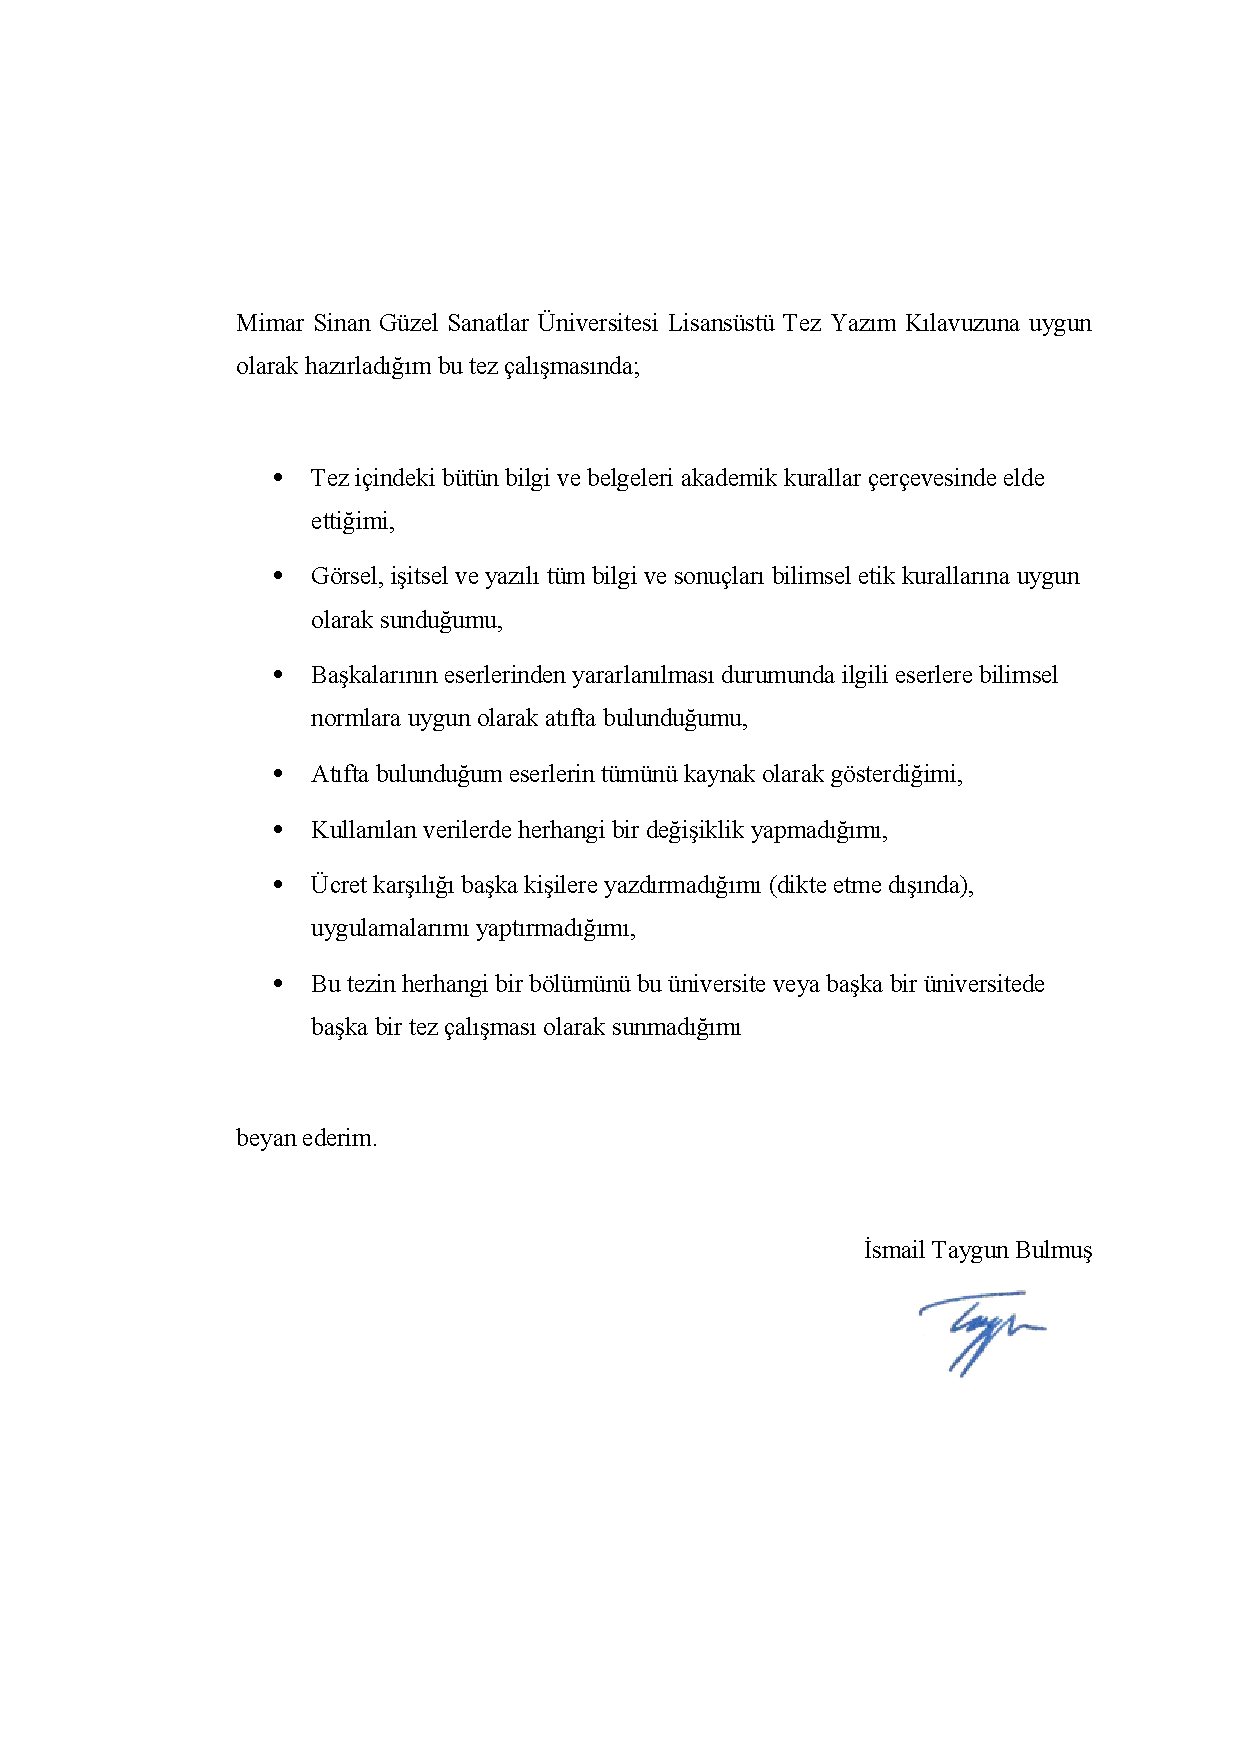
\includepdf[pages=-]{islakImzaliKagitlar/IsmailTaygunBulmus_EtikBeyanSayfasi_Imzali.pdf} 
%\includegraphics{IsmailTaygunBulmus_DoktoraTezi_ImzaKagidi.pdf}
\newpage

% Configurations --------------------------------------------------
\titleformat{\chapter}{\Large\bfseries}{\thechapter}{12pt}{}
\titleformat{\section}{\large\bfseries}{\thesection}{12pt}{}
\titleformat{\subsection}{\large\bfseries}{\thesubsection}{12pt}{}
\titleformat{\appendix}{\Large\bfseries}{\appendix}{12pt}{}
\titleformat{\tableofcontents}{\Large\bfseries}{\tableofcontents}{12pt}{}
\titleformat{\listoffigures}{\Large\bfseries}{\thelistoffigures}{12pt}{}
%\titleformat{\listofsymbols}{\Large\bfseries}{\thelistoffigures}{14pt}{}
\frontmatter
% -----------------------------------------------------------------

%%%%%%%%%%%%%%%%%%%%%%%%%%%%%%%%%%%%%%%%%%%%%%%%%%%%%%%%%%%%%%%%%%%%
% Özet
%%%%%%%%%%%%%%%%%%%%%%%%%%%%%%%%%%%%%%%%%%%%%%%%%%%%%%%%%%%%%%%%%%%%
\chapter*{\begin{center}\bfseries\large
KOLLEKTİF EVRİLEN NÖTRİNOLARIN ÇEŞNİ DÖNÜŞÜMÜ\\
(Doktora Tezi)\\
İsmail Taygun BULMUŞ\\
\vspace{0.5cm}
MİMAR SİNAN GÜZEL SANATLAR ÜNİVERSİTESİ\\
FEN BİLİMLERİ ENSTİTÜSÜ\\
Haziran 2022\\
\vspace{0.5cm}
ÖZET
\vspace{0.1cm}
\end{center}}
\addcontentsline{toc}{chapter}{ÖZET}

Nötrinolar evrende var olan diğer parçacıklarla çok küçük tesir kesitleri ile etkileşirler. Buna karşın çekirdek çökmeli süpernova (ÇÇSN) gibi bir çok astrofiziksel fenomeni açıklamada kritik rol oynarlar. Bu tezde ÇÇSN içindeki nötrino çeşni evrimini inceledik ve iki çeşni yaklaşıklığı altında kollektif çeşni evrimini veren analitik sonuçlar elde ettik. 
Madde ortamından geçerken meydana gelen MSW rezonansını ve manyetik alandan kaynaklanan SFP rezonansını detaylıca çalıştık. 
İki seviyeli sistemler için yazılan Landau-Zener (LZ) geçiş olasılıklarını yoğunluk operatörünün evrimine dahil edip sayısal simülasyonlar ile karşılaştırdık. Yoğunluk operatörüne gelen fazları başlangıç koşullarındaki küçük değişiklikler dahilinde inceleyip ortalama yoğunluk operatörünün analitik ifadesini elde ettik. SN1987A ÇÇSN modelinin $t=1-3 $ s arasındaki madde profili dikkate alındığında öngörüler ve sayısal sonuçlar uyumlu çıkmaktadır. $ t=4$ saniyeden sonra, özellikle yüksek enerjilerde, MSW ve SFP rezonansları birbirine yakınlaşır. Bu etki iki çeşni yaklaşıklığının geçerliliğini azaltır. Bu analitik sonuçların geçerlilik koşullarını efektif karışım açılarından ürettik. Ardından şok dalgası dahil edilmiş gerçekçi ÇÇSN modeli kullanıp öz-kırılım etkisini dahil ettiğimizde, antinötrinoların enerji spektrumunda oluşan spektral ayrışmanın kaybolduğunu ve elektron antinötrinolarının ısındığını bulduk. Son olarak nötrinoların ÇÇSN içerisindeki çekirdek sentezlenmesindeki rolüne baktık ve nötrino çekirdek sentezlenmesi dahil edildiğinde lityum ve bor bolluklarının arttığını bulduk. 

\begin{description}\itemsep0.05pt
%\item[Bilim Kodu:] 123
\item[Anahtar Kelimeler:] Nötrino Çeşni Salınımı, LZ geçiş olasılığı, Süpernova. 
\item[Sayfa Adedi:] 131
\item[Tez Yöneticisi:] Prof. Dr. Yamaç PEHLİVAN
\end{description}
%\clearpage

\chapter*{\begin{center}\bfseries\large
FLAVOR TRANSFORMATIONS OF COLLECTIVE EVOLVED NEUTRINOS\\
(Ph.D. Thesis)\\
İsmail Taygun BULMUŞ\\
\vspace{0.5cm}
M\.{I}MAR S\.{I}NAN FINE ARTS UNIVERSITY\\
INSTITUTE OF SCIENCE AND TECHNOLOGY\\
June 2022\\
\vspace{0.5cm}
SUMMARY
\end{center}}
\addcontentsline{toc}{chapter}{SUMMARY}

Neutrinos interact with other particles in the universe with very small cross-sections. However, they play a critical role in explaining many astrophysical phenomena, such as core collapsed supernovae (CCSN). In this thesis, we considered flavor evolution of neutrinos in a CCSN and obtained analytical results that give the collective flavor evolution under the two flavor approximation. We studied the MSW resonance that occurs when passing through the matter and the SFP resonance caused by the magnetic field. We included the Landau-Zener (LZ) transition probabilities which are valid for two-level systems in the evolution of the density operator and compared results with numerical simulations.We obtained the analytical expression of the average density operator by examining the phases of the density operator with small changes in the initial conditions. Considering the baryon profile of the SN1987A CCSN model between $t=1-3 $ s, the predictions and numerical results are compatible. After $ t=4$ second, especially at high energies, the MSW and SFP resonances become closer together. This effect reduces the validity of the two-flavor approximation. We generated the validity conditions for our analytical results in terms of effective mixing. Then, we found that when we include the self-refraction effect using the parametric shock wave included CCSN model, the spectral split in the energy spectrum of the antineutrinos disappeared and the electron antineutrinos got warmer. Finally, we looked at the role of neutrinos in nucleosynthesis in the CCSN. We looked at its role in nucleosynthesis in the CCSN and found that lithium and boron abundances increased when neutrino process is included.

\begin{description}\itemsep0.05pt
\item[Key Words:] Neutrino Flavor Evolution, LZ Transition Probability, Supernovae.
\item[Page Number:] 131
\item[Supervisor:] Prof. Dr. Yamaç PEHLİVAN
\end{description}
%\clearpage

\newpage


%%%%%%%%%%%%%%%%%%%%%%%%%%%%%%%%%%%%%%%%%%%%%%%%%%%%%%%%%%%%%%%%%%%%
% Teşekkür
%%%%%%%%%%%%%%%%%%%%%%%%%%%%%%%%%%%%%%%%%%%%%%%%%%%%%%%%%%%%%%%%%%%%
\chapter{TEŞEKKÜR}

\paragraph{}
Bu çalışmanın ortaya çıkmasında büyük emeği olan ve her konuda bana destek olan danışmanım Prof. Dr. Yamaç Pehlivan'a sonsuz teşekkürlerimi sunarım. 

\paragraph{}
Her anımda bana destek olan, yüreklendiren ve hayatımı kolaylaştıran sevgili eşim Melisa Yılmaz'a ve varlığı ile beni rahatlatan kedim Mirket'e çok teşekkür ederim. Beni ben yapan canım anneme ve babama, önümü aydınlatıp, her düştüğümde beni kaldıran en yakın dostum abime, desteğini hiç esirgemeyen yengeme ve bu Dünya'yı güzel kılan yeğenlerim Selin'e ve Aylin'e sonsuz teşekkür ederim.

\paragraph{}
Aynı anda MSGSÜ Fizik bölümüne girip, senelerce beraber dirsek çürüttüğüm dostum Mehmet Helva'ya, İTÜ ve MSGSÜ Fizik bölümündeki tüm çalışma arkadaşlarıma, sayısal hesaplama ve dostluk konusunda hep yanımda olan Burak Atakanı'ya, GSI'a gitmemi sağlayan Tuğba Arıcı'ya, bana kefil olan ve bu konuyu hiç açmayıp başaracağıma inanan Pınar Gerçek'e, Gökhan Kolutek'e ve Ceyhun Andaç'a teşekkürü bir borç bilirim.

\paragraph{}
Bu tez, Türkiye Bilimsel ve Teknolojik Araştırma Kurumu (TÜBİTAK), \\1059B141700406 numaralı 2214A projesi ile desteklenmiştir. Bu araştırmada yer alan kısmi sayısal hesaplamalar TÜBİTAK ULAKBİM, Yüksek Başarım ve Grid Hesaplama Merkezi’nde (TRUBA kaynaklarında) gerçekleştirilmiştir.
\paragraph{}
17/06/2022 \hfill İsmail Taygun Bulmuş 

%%%%%%%%%%%%%%%%%%%%%%%%%%%%%%%%%%%%%%%%%%%%%%%%%%%%%%%%%%%%%%%%%%%%
% İçindekiler
%%%%%%%%%%%%%%%%%%%%%%%%%%%%%%%%%%%%%%%%%%%%%%%%%%%%%%%%%%%%%%%%%%%%
\newpage
\tableofcontents
\cleardoublepage
\phantomsection % For hyperref

%%%%%%%%%%%%%%%%%%%%%%%%%%%%%%%%%%%%%%%%%%%%%%%%%%%%%%%%%%%%%%%%%%%%
% Tablo Listesi
%%%%%%%%%%%%%%%%%%%%%%%%%%%%%%%%%%%%%%%%%%%%%%%%%%%%%%%%%%%%%%%%%%%%
\clearpage
\renewcommand\cftlottitlefont{\Large \textbf}
\listoftables

%%%%%%%%%%%%%%%%%%%%%%%%%%%%%%%%%%%%%%%%%%%%%%%%%%%%%%%%%%%%%%%%%%%%
% Şekil Listesi
%%%%%%%%%%%%%%%%%%%%%%%%%%%%%%%%%%%%%%%%%%%%%%%%%%%%%%%%%%%%%%%%%%%%
\clearpage
\renewcommand\cftloftitlefont{\Large \textbf}
\listoffigures


%%%%%%%%%%%%%%%%%%%%%%%%%%%%%%%%%%%%%%%%%%%%%%%%%%%%%%%%%%%%%%%%%%%%
% Sembol Listesi
%%%%%%%%%%%%%%%%%%%%%%%%%%%%%%%%%%%%%%%%%%%%%%%%%%%%%%%%%%%%%%%%%%%%
%\renewcommand*{\arraystretch}{1.37}
\chapter{SEMBOL LİSTESİ}
\begin{longtable}{@{}l @{\hspace{10mm}} l }
$ c_{\alpha}            $ &: $\cos \alpha$ \\
$ s_{\alpha}            $ &: $\sin \alpha$ \\
$ r                     $ &: Uzaklık \\
$ E                     $ &: Enerji \\
$ m_{i}                 $ &: Nötrino Kütlesi \\
$ \delta m^{2}          $ &: Nötrino Kütle Kare Farkı \\
$ \Delta                $ &: $\delta m^{2}/4E$ \\
$ \mu                   $ &: Nötrino Dipol Momenti \\
$ \hat{H}^{f}           $ &: Çeşni Tabanında Hamiltonyen Operatörü\\
$ \hat{H}^{k}           $ &: Kütle Tabanında Hamiltonyen Operatörü\\
$ \hat{H}^{M}           $ &: Madde Tabanında Hamiltonyen Operatörü\\
$ P_{\nu_{\alpha}\rightarrow\nu_{\beta}}$ &: $ \alpha $ Çeşnisinden $ \beta $ Geçiş Olasılığı \\
$ P_{\nu_{\alpha}\rightarrow\nu_{\alpha}}$ &: $ \alpha $ Çeşnisine Sahip Olan Nötrinonun Yaşama Olasılığı\\
$ A                     $ &: Geçiş Genliği\\
$ \ket{\Psi(r)}         $ &: Nötrino Durum Keti\\
$ \ket{\nu_{\alpha}}    $ &: Çeşni Tabanında Nötrino Keti, $ \alpha = e,x,\overline{e},\overline{x} $ \\
$ \ket{\nu_{i}}         $ &: Kütle Tabanında Nötrino Keti, $ i = 1,2,3,4 $ \\
$ \ket{\nu_{i}^{M}}     $ &: Madde Tabanında Nötrino Keti, $ i = 1,2,3,4 $ \\
$ \ket{\nu_{i}^{EM}}    $ &: Elektromanyetik Tabanında Nötrino Keti, $ i = 1,2,3,4 $ \\
$ \theta                $ &: Boşluk Karışım Açısı \\
$ \theta_{M}            $ &: Nötrinolar İçin Efektif Madde Karışım Açısı \\
$ \overline{\theta}_{M} $ &: Antinötrinolar İçin Efektif Madde Karışım Açısı \\
$ \gamma                $ &: $\theta_{M}-\overline{\theta}_{M}$ \\
$ \theta_{EM}           $ &: Efektif Elektromanyetik Karışım Açısı \\
$ \mathcal{R}           $ &: Dönme Matrisleri \\
$ U                     $ &: Boşluk Dönüşüm Matrisi \\
$ U_{M}(r)              $ &: Efektif Madde Dönüşüm Matrisi \\
$ U_{EM}(r)             $ &: Efektif Elektromanyetik Dönüşüm Matrisi \\
$ \lambda^{\nu}_{i}     $ &: Boşluk Salınım Hamiltonyen'in Özdeğerleri, $ i = 1,2,3,4 $ \\
$ \lambda^{\nu,EM}_{i}  $ &: Boşluk Salınım ve Elektromanyetik Hamiltonyen Toplamlarının \\
& Özdeğerleri, $ i = 1,2,3,4 $ \\
$ \lambda_{i}           $ &: Boşluk Salınım, Madde ve Elektromanyetik Hamiltonyen Toplamlarının \\
& Özdeğerleri, $ i = 1,2,3,4 $ \\
$ \omega_{i}            $ &: Madde Hamiltonyen'in Özdeğerleri, $ i = 1,2,3,4 $ \\
$ V_{NC}(r)             $ &: Efektif Yüksüz Akım Potansiyeli \\
$ V_{CC}(r)             $ &: Efektif Yüklü Akım Potansiyeli \\
$ G_{f}                 $ &: Fermi Çiftlenim Sabiti \\
$ N_{e}                 $ &: Elektron Yoğunluğu \\
$ N_{n}                 $ &: Nötron Yoğunluğu \\
$ N_{p}                 $ &: Proton Yoğunluğu \\
$ N_{b}                 $ &: Baryon Yoğunluğu \\
$ Y_{e}                 $ &: Elektron Kesri \\
$ Y_{n}                 $ &: Nötron Kesri \\
$ B                     $ &: Manyetik Alan \\
$ P_{LZ}                $ &: Landau - Zener Geçiş Olasılığı \\
$ \Gamma                $ &: Adyabatisite \\
$ \vec{B}               $ &: Bloch Vektörü \\
$ \vec{\sigma}          $ &: Pauli-spin Matris Vektörü
\end{longtable}

\newpage

%%%%%%%%%%%%%%%%%%%%%%%%%%%%%%%%%%%%%%%%%%%%%%%%%%%%%%%%%%%%%%%%%%%%
% Kısaltma Listesi
%%%%%%%%%%%%%%%%%%%%%%%%%%%%%%%%%%%%%%%%%%%%%%%%%%%%%%%%%%%%%%%%%%%%
%\renewcommand*{\arraystretch}{1.37}
\chapter{KISALTMA LİSTESİ}
\begin{longtable}{@{}l @{\hspace{10mm}} l } 
ÇÇSN  &: Çekirdek Çökmeli Süpernova \\
LZ  &: Landau - Zener \\
MSW  &: Mikheev, Smirnov ve Wolfenstein \\
SFP  &: Spin Çeşni Yalpalama (Spin Flavor Precession) \\
YMYG &: Yarım Maksimumdaki Yarım Genişlik (Half Width At Half Maksimum)\\
PUSH &: Parametrized Spherically Symmetric Explosion Method \\ 
NİD &: Nükleer İstatistiksel Denge
\end{longtable}
\newpage

% Configurations --------------------------------------------------
\mainmatter
\pagestyle{plain}
\setlength{\baselineskip}{1.5\baselineskip}
% -----------------------------------------------------------------

\newpage
\chapter{GİRİŞ}\label{ch:giris}

% GİRİŞ
Astrofiziksel nötrinolar hem nötrinoların temel özelliklerini hem de çekirdek-çökmeli süpernovalar (ÇÇSN) gibi astrofiziksel fenomenleri anlamamızı sağlayan, bilinen en hafif atom altı parçacıklardır \cite{Janka:2006fh, Janka:2012wk, Burrows:2012ew}. Laboratuvar ortamında nötrinoların özelliklerini belirlemeye çalışan deneyler olmasına rağmen, bu deneylerin çoğu sadece fiziksel niceliklerin üst sınırını belirler. Bu üst sınırlar, mesela nötrino manyetik momenti gibi, astrofiziksel olayların tüm fiziğini anlamak için yeterli değildir \cite{Brdar:2020quo, Super-Kamiokande:2020frs}. Bu nedenle astrofiziksel fenomenleri anlayabilmek için çok çeşitli nötrino çeşni (flavor) salınım simülasyonları yapılmalıdır.

% NÖTRİNO PARÇACIĞI
Standart model'de kütlesiz olarak öngörülen nötrinoların kütlesinin olduğu birçok deneyle ispatlanmıştır \cite{Gonzalez-Garcia:2007dlo,ParticleDataGroup:2018ovx}. Sadece zayıf etkileşimler sonucu ortaya çıkan nötrinoların çeşnisi beraber meydana geldiği lepton tarafından belirlenir. Zayıf etkileşimler sonucunda ortaya çıktığında çeşnisi belli olan nötrinolar boşlukta kütle özbazında (eigenbasis) ilerler. Bu da nötrinoların çeşnisinin salınımına sebep olur \cite{Super-Kamiokande:1998kpq, Maltoni:2004ei,LSND:2001aii,SNO:2002tuh, T2K:2017hed}. Bu durum en az bir nötrino kütle değerinin sıfırdan farklı olduğu durumda geçerlidir \cite{Giunti:2007ry}.

% NÖTRİNO ÇEŞNİ SALINIMI
Nötrino salınım fikrini 1950 yılında ilk olarak ortaya atan kişi Pontecorvo'dur \cite{Pontecorvo:1957cp}. Pontecorvo, laboratuvarda üretilen kaon adlı parçacığın antikaon'a salınmasından esinlenmiştir. Maki, Nakagawa ve Sakata, 1970 tarihinde yazdıkları makalede, nötrinoların antinötrinolara değil kendi çeşnileri arasında salınım yapabileceğini öne sürmüştür \cite{Maki:1962mu}. Evrendeki toplam çeşni sayısı, Standart Model'in öngörüsüne göre üçtür \cite{ParticleDataGroup:2018ovx} ve nötrino çeşnisi, tanımlanan bu üç kuantum büyüklük arasında salınır. Analitik hesaplar yapılırken üç seviyeli sistemler incelemek yerine iki seviyeli sistemlerin incelenmesi daha kullanışlıdır. Bu yaklaşıklık, hem hesap kolaylığı açısından önemlidir hem de kollektif çeşni evrimi gibi işlemci saati harcayan karmaşık sistemleri çözerken zaman kazandırır \cite{Duan:2010bg, Mirizzi:2015eza}. Bu tezin bazı noktalarında üç çeşnili evrim yapısına değinilecektir ancak elde ettiğimiz tüm hesaplar iki çeşni yaklaşıklığı ile yapılacaktır. Ayrıca nötrino salınım teorisi bilinen üç çeşniden daha fazla "çeşninin" varlığında da geçerlidir. Standart Model'de olmayan bu yeni çeşnili nötrinolara steril nötrinolar adı verilir. Bu tezde steril nötrino hesaplarına değinilmemiştir.

% SÜPERNOVA ORTAMI
1987 Yılında Büyük Macellan Bulutu içerisinde bir süpernova meydana gelmiştir ve bu astrofiziksel olay Dünya'dan gözlenmiştir. Gerçekleşen bu süpernova'ya SN1987A adı verilmiştir. O dönemde proton yarılanma süresi gibi fiziksel olayları incelemek için kullanılan deneyler, SN1987A optik gözlemlerinden birkaç saniye önce olağan dışı nötrino yoğunluğu gözlemlemişlerdir \cite{1987Natur.330..142S, 1987PhRvL..58.1490H}. Güneş nötrino gözlemlerini saymazsak, ilk defa kaynağı bilinen bir astrofiziksel fenomenden foton dışında bir parçacık gözlemlenmiştir.

SN1987A nötrino gözlemlerinin ardından süpernova fiziği araştırmaları hız kazanmış ve bu konuda sayısız araştırma yapılmıştır (\cite{Janka:2006fh} numaralı derlemeye ve bu derlemenin referanslarına bakınız.) Süpernova fiziği çok boyutlu, dinamik değişkenli ve başlangıç parametrelerine sıkı bağlı olduğundan dolayı simülasyonların gerçekleştirilmesi veya "patlatılması" epeyce zordur. Bunun için az da olsa deneysel veriye sahip olduğumuz SN1987A yapısını modelleyen sistemler kullanılmaktadır. Bu tezde geçen süpernova kelimesi ÇÇSN kelimesi yerine kullanılmıştır. ÇÇSN oluşumunun adımları kısaca şöyle özetlenir. Füzyon reaksiyonlar sonucu soğan yapısında olan Yıldız'ın çekirdeğinde demir/nikel bölgesi bulunmaktadır. Yüksek basınç ve sıcaklığa rağmen zincirleme füzyon reaksiyonu demir çekirdeğinde durur. Bunun sebebi demir/nikel çekirdeğinin aşırı stabil olmasıdır. Bu çekirdekler ile zincirleme füzyon reaksiyonu meydana gelmez. Başka bir dille ifade edersek, çekirdek başına düşen ortalama bağlanma enerjisi en yüksek çekirdek demirdir. Füzyon reaksiyonunun durduğu Yıldız'ın merkezinde, dışarıya doğru basınç kalmayınca içe doğru çöküş başlar (collapse.) Çöküşün başlamasının ardından Yıldız'ın merkezinde yaklaşık $ 10 $ km yarıçapında, biriken madde nükleer yoğunluğa erişir ve elektron dejenerasyon basıncı çöken maddenin daha fazla çökmesine izin vermez. Bu durumda çöken madde geri seker (bouncing.) Sekme sonucunda şok dalgası oluşur (shock formation) ve merkezden dışarı doğru madde aktarımı başlar. Ardından Yıldız'ın merkezinden çok büyük miktarda nötrino ve antinötrino açığa çıkar (neutrino burst.) Çok yüksek miktarda parlaklığa sahip olan nötrinolar Yıldız içerisinde biriken enerjinin yüzde $ 99 $'unu dışarıya taşır. Nötrinolar dışarı doğru giderken şok dalgasını "ısıtır" ve "iter" (neutrino heating.) Şok dalgası belli bir limit hıza eriştikten sonra patlama "gerçekleşti" denilir. Ardından açığa çıkan muazzam miktardaki nötrino Yıldız'ın içerisindeki enerjiyi dışarıya çıkartır (cooling.). Patlamanın başlangıcı sekmenin olduğu zaman dilimi olarak kabul edilir. Bu çalışmadaki nötrinoların kollektif çeşni evrimi ÇÇSN'nin soğuma evresinde incelenecektir. Soğuma evresi ise patlamanın başlangıcından yaklaşık bir saniye ile on saniye arasındaki dönemi kapsar. 

Süpernova sırasında Yıldız çekirdeğinde bulunan proto-nötron yıldızının manyetik alanı olabilir. Bu durumda süpernova simülasyonu yapılırken dinamik manyeto -hidrodinamik denklemler de çözülmelidir \cite{1970ApJ...161..541L, 2011ApJ...743...30T, Burrows:2012ew}. Çekirdeğin oluşturduğu manyetik alan, foto-ayrışma (photodissocciation) mekanizmasını etkileyerek şok dalgasının ilerlemesine ve ısınmasına yardımcı olur. Oluşan manyetik alan dinamik bir yapıya sahiptir ve zamana bağlı olarak değişmektedir. Bu tezde nötrino çeşni evrimi incelenirken bu manyetik alanın statik olduğu varsayılacaktır. Literatürde,statik manyetik alanın sabit değerde olduğu \cite{Abbar:2020ggq}, uzaklığın karesi ile ters orantılı olduğu \cite{Kharlanov:2020cti,deGouvea:2012hg, deGouvea:2013zp} ve uzaklığın üçüncü kuvveti ile ters orantılı \cite{Sasaki:2021bvu} olduğu yaklaşımlar bulunmaktadır. Bu tezde kullanılacak olan manyetik alan uzaklığın karesi ile ters orantılı olarak değişecektir.

% NÖTRİNO ELEKTROMANYETİK ETKİLEŞİM
Nötrinoların çeşni evrimi Yıldız içerisinde oluşan manyetik alandan etkilenmektedir \cite{Giunti:2014ixa}. Bu etkileşimin yapısı nötrinolar ile madde etkileşiminden farklı olarak gelecektir, çünkü nötrinolar yüksüz oldukları için foton ile etkileşmezler. Standart Model'in minimal bir genişlemesi yazıldığında, nötrino ile fotonu birinci mertebeden tedirgeme diyagramları ile etkileştirmek mümkündür \cite{Pal:1981rm}. Bu durumdan kaynaklı nötrinoların çok küçük değerli manyetik dipol momenti oluşacaktır. Standart Model'i, nötrino kütlesi kullanarak genişlettiğimizde nötrino manyetik momenti için elde edilen değer $ 10^{-19} $ Bohr magnetonu ($ \mu_{B} $) değerinden düşüktür \cite{Marciano:1977wx, Shrock:1982sc, Raffelt:1996wa, Bell:2005kz, Bell:2006wi}. Nötrino elektromanyetik etkileşimler nötrinonun doğasına bağlı olarak da farklılık gösterecektir. Eğer nötrinolar Dirac doğasında ise Standart Model'e göre nötrinolar sadece sol elli (left handed) olmalı, sağ elli anti-partneri olmalıdır. Dirac nötrinosunun deneylerle belirlenen manyetik dipol moment üst sınır değerleri \ref{fig:mu_nu} numaralı şekilde verilmiştir. Majorana nötrinolarında ise Dirac nötrinolarından elde edilen manyetik momentin sadece köşegen elemanları bulunacaktır. Hem Dirac doğası hem de Majorana doğasında nötrino manyetik momentinin tanımı model bağımlıdır. Bu tezde sadece Majorana nötrinoları dikkate alınmış olup nötrino manyetik momentinin $ \mu_{\nu}=5\times10^{-16} \mu_{B}$ değerinde olduğu kabul edilmiştir. Bu değer literatürde kullanılan ve deneylerden elde edilen büyüklüklerle uyumludur \cite{Bell:2006wi, Kuroda:2020pta, Super-Kamiokande:2020frs, Borexino:2017fbd, Brdar:2020quo}.

\begin{figure}[hbt!]
    \centering
    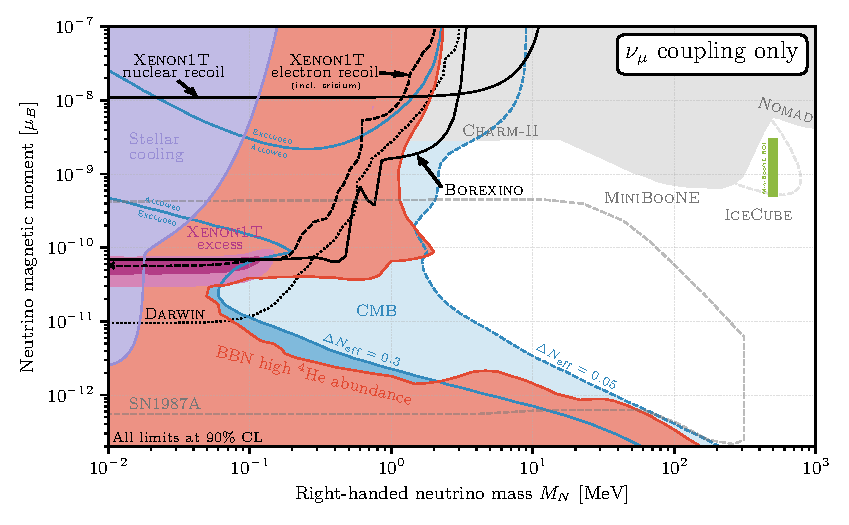
\includegraphics[width=\textwidth]{figures/Brdar_2020quo_mn_vs_munu_summary.pdf}
    \caption[Nötrino Manyetik Momentinin Üst Sınır Değerleri.]{Nötrino Manyetik Momentinin Üst Sınır Değerleri. Bu şekil \cite{Brdar:2020quo} numaralı kaynaktan alınmıştır.}
    \label{fig:mu_nu}
\end{figure}

% NÖTRİNO ÖZ KIRILIMI
ÇÇSN soğuma evresinde açığa çıkan nötrinolar hem cinsleri ile de etkileşecektir. Dikkate alınan test nötrinosu ÇÇSN ile açığa çıkan nötrino gazı ile etkileşime girecektir. Bu etkileşim terimleri yazılırken ortalama alan yaklaşıklığı kullanılmaktadır \cite{Sigl:1993ctk, Volpe:2015rla}. Nötrinoların bu tip etkileşimlerine nötrino öz-kırılımı (self-refraction) adı verilir. ÇÇSN'nın erken zamanında en önemli kollektif etki, nötrino öz-kırılımından gelir \cite{Duan:2006an, Duan:2008fd, Pehlivan:2011hp, Volpe:2013uxl}. Bu konu hakkında yapılan çalışmalar için \cite{Duan:2010bg} numaralı derleme makalesine bakınız.

% REZONANSLAR
Boşluktaki nötrino çeşni salınımlarında salınım genliği ve salınım frekansı değişmez. Nötrinoların çeşni evrimini etkileyen bir dış etki varsa, salınım frekansı ve genliği, o dış etkinin yapısına göre değişecektir. Eğer dış etki evrim sırasında değişmez kalırsa çeşni salınımlarının frekansı ve genliği de sabit kalacaktır. Bu dış etken nötrino-madde etkileşimi veya nötrino-manyetik alan etkileşimi olabilir.

Dış etkinin zamanla değişmesi durumunda ise çeşni salınım frekansı ve genliği değişimden etkilenecektir. Etkinin değişmesinden kaynaklanan salınım frekansı ile nötrino boşluk salınım frekansında bir uyum sağlanır ise çeşni salınımlarında ani bir değişim meydana gelecektir. Bu ani değişim sadece belli frekanslarda oluşur. Bu fenomene genel olarak \emph{rezonans} adı verilir. Bu özel frekansa ise \emph{rezonans frekansı} adı verilir. Rezonans fenomeni, doğal olarak salınım hareketi yapan sistemlere dış etki tarafından uygulandığında oluşabilir.

Madde içerisinde salınan nötrinoların rezonansa girebileceği ilk olarak Mikheev, Smirnov ve Wolfenstein tarafından bulunmuştur \cite{Wolfenstein:1977ue, Mikheyev:1985zog}. Bu fenomene de MSW rezonansı adı verilmiştir. Wolfenstein'ın madde içerisinde nötrino salınımları üzerine makalesinin yayınlamasının ardından Mikheev ve Smirnov Güneş içerisinde oluşan nötrinoların rezonansa girdiğini bulmuş ve literatürde solar nötrino problemi olarak adlandırılan sorun çözülmüştür. Bu çözüm Dünya'da yapılan deneylerle ispatlanmıştır \cite{Bellerive:2016byv}.

Nötrinoların madde içerisinden geçerken MSW rezonansına girmesi gibi manyetik alan içerisinden geçerken de salınımları rezonansa girebilir. Bu rezonansa SFP (spin-flavor precession) rezonansı adı verilir \cite{Okun:1986na, Fujikawa:1980yx, Cisneros:1970nq,Akhmedov:1988uk,Akhmedov:1987nc,Lim:1987tk}. SFP rezonansı nötrino manyetik momenti ve dış manyetik alan ile orantılıdır. Rezonansa girme koşulları büyük oranda MSW rezonansına benzemektedir. Bu rezonansın MSW rezonansından en büyük farkı nötrino-antinötrino geçişlerine olanak sağlamasıdır. 

% Bizim Yaptıklarımız
Bu tezde, nötrino-elektromanyetik etkileşimi varlığında elde ettiğimiz analitik sonuçları çeşni evrimini veren diferansiyel denklemin sayısal sonuçları ile karşılaştırıp bunların çoğunlukla uyumlu olduğunu ve uyumlu olması için gerekli şartların neler olduğunu gösterdik. Elde ettiğimiz şartlar dahilinde çeşni evrimini betimleyen yoğunluk operatörünün analitik ifadesini elde ettik. Bu analitik/sayısal karşılaştırmalarında öz-kırılım potansiyelini ihmal ettik, çünkü nötrino öz-kırılımı sistemi doğrusal olmayan hale getirmektedir. Karşılaştırmayı yaparken sayısal çözümlerdeki başlangıç koşullarını küçük oranda rastgele değiştirip kuantum fazlarından kaynaklanan farklılıkların açığa çıkmasını sağladık. Elde ettiğimiz analitik formülü bu fazlardan kaynaklanan değişimi kapsayacak şekilde yazdık. Analitik öngörümüz iki farklı rezonansın birbirinden ayrıldığı noktalarda geçerli olacaktır. Rezonansların birbirinden ne kadar ayrı olması gerektiğini nitel birkaç büyüklük tanımlayarak belirledik. Rezonansların birbirinden yeteri kadar ayrı olduğu durumlarda analitik öngörümüz sayısal sonuçlarımızla tutarlı sonuçlar vermektedir.

Bu tezin ikincil çıktıları ise şunlardır: Nötrino elektromanyetik etkileşimi ve nötrino madde etkileşimi varlığında yazılan hareket denklemini tedirgeme yöntemi kullanarak çözdük. Tedirgeme kuramından özvektörleri ve enerjiye gelen katkıları elde ettik. Buna ek olarak efektif iki çeşni yaklaşıklığı kullanıp sabit ve eksponansiyel manyetik alan için tam analitik çözümler elde ettik. Ayrıca gerçekçi ÇÇSN modeli için sayısal simülasyonlar yaptık. Bu simülasyonlarda nötrino öz-kırılımı ve ÇÇSN şok dalgası sisteme dahil edilmiştir. Son olarak PUSHing adlı parametrik ÇÇSN modeli kullanarak nötrinolardan kaynaklanan çekirdek sentezi ağ denklemlerini çözdük. Nötrino etkileşimlerinin ÇÇSN içerisinde nu-işlem elementlerininin bolluğunu arttırdığını belirledik.

% TEZİN İÇİNDEKİ BÖLÜMLER
Tezin planı şöyledir: İkinci bölümünde nötrino hareket denklemleri, boşluk salınımları ve dış ortamla etkileşimleri incelenmiştir. Nötrino evrimini betimleyen hareket denklemleri verildikten sonra boşluktaki çeşni salınımları için hareket denklemleri çözülmüştür. Madde ortamında çeşni salınımı yapan nötrinoların hareket denklemleri incelenmiş ve efektif açı yaklaşıklığı kullanılarak çözümler elde edilmiştir. Ardından elektromanyetik alan içerisinde hareket eden nötrinoların hareket dinamikleri belirlenmiş ve madde etkileşimi ile beraber alınarak hem tedirgenmiş çözümler hem de bazı profiller için analitik çözümler elde edilmiştir. Hareket kinematiğinin son bölümünde ise nötrino öz-kırılım potansiyeli elde edilmiştir.

Üçüncü bölümde ise nötrino çeşni salınımları sırasında meydana gelen rezonans durumlarına değinilmiştir. Landau-Zener (LZ) formülü kullanılarak geçiş olasılıklarının genel ifadeleri incelenmiş, ardından MSW ve SFP rezonanslarının gerçekleşme koşulları yazılmıştır. Rezonans bölgeleri evrimin adyabatikliğini belirlediği için adyabatisite parametresi de bu bölümde tanımlanmıştır.

Dördüncü bölümde ise bu çalışmamızın sonuçları olan simülasyonların analitik öngörüleri ve karşılaştırmalı sonuçları yer almaktadır. Yoğunluk operatörünün özbazdaki ifadesi analitik olarak bu bölümde elde edilmiştir. Ardından ÇÇSN içerisinde ilerleyen nötrinoların başlangıç koşulları ve geometrisi belirlenmiştir. Bu tezde elde ettiğimiz analitik/sayısal sonuç karşılaştırması oyuncak model alt başlığında yer almaktadır. Son olarak gerçekçi ÇÇSN modelinde nötrino etkileşimlerinin rolleri dört farklı etkileşim modeli kullanılarak incelenmiştir.

Beşinci bölümde ise nötrinoların süpernova içerisindeki çekirdek sentezlenmesine (nucleosynthesis) olan katkısı üzerine çalışmalar bulunmaktadır. Bu bölümde PUSHing adlı süpernova simülasyonu ve çekirdek sentezleme ağı kullanılarak Lityum ve Bor izotoplarının kütle kesirleri elde edilmiştir. Nötrino işleminin veya nötrino ile sentezlemenin (nu-process), bu izotopları sentezlemede önemi ortaya konmuştur.

Çalışmalarımızın sonuçları ve tartışması sonuç bölümünde incelenmiştir.

Çalışmamızda, hem kolay sayısal hesaplamalar yapmamıza olanak sağlayan matris notasyonu hem de operatör notasyonu kullanılmıştır. Ayrıca hesaplamalarda doğal birimler kullanılmıştır. Yani ışık hızı, Plank sabiti ve Stefan Boltzman sabiti $ 1 $ alınmıştır. Gerekli olduğu yerlerde uygun dönüşümler kullanılmıştır. Buna ek olarak nötrinoların hızı ışık hızına çok yakın olduğu için (erken evren soğuk nötrinolar dışında) zaman $ t $ ve konum $ r $ eşdeğer olarak görülmüştür. Bundan dolayı zamana bağlı olarak tanımlanan denklemler yerine konumla değişen denklemler yazılmıştır.
\newpage
\chapter{NÖTRİNO SALINIM KİNEMATİĞİ}\label{ch:nuHareketKinematik}
\paragraph{}
Nötrinolar kütleli, ışık hızına yakın hızlarda giden ve Fermi-Dirac istatistiğine sahip olan parçacıklardır. Nötrinoların çeşni evrimi Schrödinger tipi denklem ile verilir \cite{Raffelt:1996wa}. 
\begin{equation}\label{eqn:NuKim_EoM_Psi}
	i\dv{r} \ket{\Psi(r)}= H^{\text{f}}(r) \ket{\Psi(r)} \text{ .}
\end{equation}
Burada $ \ket{\Psi(r)} $ nötrino durum (state) keti veya vektörü $ H^{\text{f}} $ çeşni tabanında yazılmış Hamiltonyen'dir. Hareket denklemi Schrödinger tipi diferansiyel denklem ile yazılabileceği gibi integral denklemleri şeklinde de yazılabilir \cite{Kneller:2005hf}. Bu tezde, dört ($ 2 $ nötrino, $ 2 $ antinötrino) çeşni dikkate alınacaktır. \eqref{eqn:NuKim_EoM_Psi} numaralı hareket denklemi nötrino çeşni ketlerine göre aşağıdaki gibi olur.
\begin{equation}\label{eqn:NuKim_EoM_4Mat}
	i\dv{r} \mqty(\ket{\nu_{e}(r)} \\ \ket{\nu_{\mu}(r)}\\ \ket{\nu_{\overline{e}}(r)}\\ \ket{\nu_{\overline{\mu}}(r)}) = H^{\text{f}}(r) \mqty(\ket{\nu_{e}(r)} \\ \ket{\nu_{x}(r)}\\ \ket{\nu_{\overline{e}}(r)}\\ \ket{\nu_{\overline{x}}(r)}) \text{ .}
\end{equation}
Bu denklemdeki durum vektörü, çeşni bazında yazılmıştır. $ x $ olarak etiketlenen nötrinolar müon ve tau çeşnilerinin bir kombinasyonu olarak düşünülür. Üniter dönüşümler kullanılarak \eqref{eqn:NuKim_EoM_4Mat} numaralı denklem başka bazlara çevrilebilir.

Astrofiziksel ortamdaki parçacıkların davranışlarını tek tek incelemek imkansızdır. Bunun yerine onların toplu davranışlarını incelemek daha uygun olur. Bunun için nötrino parçacığının evrimini veren Schrödinger denklemini çözüp durum vektörünü elde etmek yerine yoğunluk operatörü formalizmine geçilir. Yoğunluk operatörü formalizmi nötrinoların istatistiksel dağılımının evrimine bakabilmemize olanak verir. \eqref{eqn:NuKim_EoM_Psi} numaralı denklemin $ \ket{\Psi_{1}(r)} $ için yazıldığını varsayalım. Ardından \eqref{eqn:NuKim_EoM_Psi} numaralı denklemi sağdan $ a_{1}\bra{\Psi_{1}(r)} $ ile çarpalım. Aynı işlemi $ \ket{\Psi_{2}(r)} $ için de yapıp alt alta $ i $ kere toplarsak aşağıdaki ifadeyi elde ederiz.
\begin{equation}
	i\dv{r} \qty(\sum_{i} a_{i} \dyad{\Psi_{i}(r)}{\Psi_{i}(r)})  = \comm{H^{\text{f}}(E,r)}{\sum_{i} a_{i} \dyad{\Psi_{i}(r)}{\Psi_{i}(r)} } \text{ .}
\end{equation}

Artık yoğunluk operatörünü tanımlayabiliriz.
\begin{equation} \label{eqn:NuKim_YogOperatorTanım}
	\hat{\rho} (r) = \sum_{i} a_{i} \dyad{\Psi_{i}(r)}{\Psi_{i}(r)}  \text{ .}
\end{equation}
Burada $ a_{i} $ bir sayıdır ve sistemde ne oranda $ \ket{\Psi_{i}(r)} $ durumu olduğunu betimler. Yani iki durumlu sistem için $ a_{1}=N_{1}/(N_{1}+N_{2}) $ şeklinde yazılır. Yoğunluk operatörünü hareket denklemine koyduğumuzda \emph{Liouville - von Neumann} denklemini elde ederiz. 
\begin{equation}\label{eqn:NuKim_LiouvilleVonNeumann}
	i \dv{r} \hat{\rho} = \comm{\hat{H}}{\hat{\rho}} \text{ .}
\end{equation}
Bu denklem Heisenberg Denklemine benzemektedir ancak Liouville - von Neumann denkleminde operatörler değil durumlar evrilir. Buna ek olarak eksi işaret farkı da vardır. Liouville - von Neumann denkleminin sağ tarafına çarpışma (collision) katkıları da yazılabilir \cite{Volpe:2015rla}. Bu çalışmada çarpışma terimleri ihmal edilecektir. Denklemin sol tarafı ise konuma göre tam türev içerir. Yani $ \dv{r} = \pdv{r} + \vec{v} \cdot \vec{\nabla} $ şeklinde yazılır. Bu çalışmada yoğunluk operatörü açıdan bağımsız bir şekilde evrilecektir. Bundan dolayı hız, $ \vec{v} $, ile bağlı olan tüm terimler düşecektir. Geometri hakkında ayrıntılı bilgi için \ref{subsec:geometri} numaralı bölüme bakabilirsiniz.

Yoğunluk operatöründen yoğunluk matrisine geçmek için bir baz seçilmesi gerekmektedir. Örneğin, çeşni bazını, $ \ket{\nu_{\alpha}} $, ele alalım. Bunun için \eqref{eqn:NuKim_YogOperatorTanım} numaralı denkleme iki adet tam küme (complete set) koymamız gerekir.
\begin{equation}
	\hat{\rho}(r) = \sum_{\alpha,\beta} \rho_{\alpha\beta}(r) \dyad{\nu_{\alpha}}{\nu_{\beta}} \text{ .}
\end{equation}
Burada $ \rho_{\alpha\beta}(r) $ yoğunluk matrisidir ve aşağıdaki gibi tanımlanır.
\begin{equation}
	\rho_{\alpha\beta}(r) = \sum_{i} a_{i}\braket{\nu_{\alpha}}{\Psi_{i}(r)}\braket{\Psi_{i}(r)}{\nu_{\beta}}
\end{equation}
$ a_{i} $, topluluğun (ensemble) içerisindeki nötrino çeşnilerinin (diğer bazlarda da tanımlanabilir) ağırlığını vermektedir. Yoğunluk matrisi tanımlanan baza göre değişiklik gösterir. Evrim ise yoğunluk operatörü ile ilişkili olduğu için seçilen bazdan bağımsızdır. Yani fiziksel evrim, seçilen bazdan bağımsızdır.

Yoğunluk matrisine örnek olarak iki durumlu nötrinoları ele alabiliriz. Örneğin, $ \ket{\nu_{e}} = \mqty(1\\0) $ ve $ \ket{\nu_{x}} = \mqty(0\\1) $ olsun. Bu durumda yoğunluk operatörü şöyle yazılır.
\begin{equation}
	\hat{\rho}(r) = \mqty(\rho_{ee}(r) & \rho_{ex}(r) \\\rho_{xe}(r) & \rho_{xx}(r)) \text{ .}
\end{equation}
Yoğunluk matrisi saf (pure) ve karışık (mixed) olmak üzere iki çeşit olabilir. Saf durumlar sadece aynı cins durumların bir araya gelmesiyle oluşur. Karışık durumlarda ise farklı kombinasyonlara sahip durumlar da olabilir. Bu çalışmada, başlangıçtaki yoğunluk matrisi her zaman saf durumda olacaktır.

Yoğunluk matrisinin temel özellikleri evrimin kavramsal olarak anlaşılmasını kolaylaştırır. Yoğunluk matrisinin izi birdir. Bu da topluluğun içerisindeki toplam maddenin korunduğu anlamına gelir. Yani toplulukta $ a_{1} $ oranında $ \ket{\Psi_{1}} $ parçacığı, $ a_{2} $ oranında $ \ket{\Psi_{2}} $ olsun. Başlangıçta $ a_{1}+a_{2} =1 $ olarak verilir. Bu toplamın evrimin her anında aynı olması beklenir. Yoğunluk matrisinin her bir köşegen elemanı ise yaşama olasılığı (survival probability) ile orantılıdır. Örneğin, saf bir durumda, yoğunluk matrisinin $ \rho_{ee}(r) $ elemanı, hayata elektron nötrinosu olarak başlayıp $ r $ uzaklığında hala elektron nötrinosu olma olasılığının $ a_{e} $ ile çarpımını verir. Benzer şekilde köşegen olmayan elemanlar da geçiş olasılığı ile orantılıdır. Yoğunluk matrisinin izinin bir olmasının yanında üst köşegen elemanları ile alt köşegen elemanları birbirinin sanal eşleniğidir (complex conjugate.) Yoğunluk matrisinin diğer özellikleri ve uygulamaları \cite{2012dmta.book.....B} numaralı kaynakta ayrıntılı olarak verilmiştir.

Nötrino durumu, $ \ket{\Psi(r)} $, başlangıçta Hamiltonyen'in özvektörleri cinsinden yazalım. Sistemin başlangıçtaki özvektörleri de $ \ket{E_{i}(R)} $ olarak gösterilsin. Burada durum, tek bir özvektöre eşit olabildiği gibi birden çok öz durumun doğrusal kombinasyonu da olabilir. Eğer nötrino durumu, evrim boyunca fazladan bir faz ile beraber Hamiltonyen'in özbazında kalıyorsa, evrime \emph{adyabatiktir} denir. Adyabatik evrimde, herhangi bir $ r $ uzaklığında nötrino durumu aşağıdaki gibi yazılır.
\begin{equation}\label{eqn:Psi_rAdiabaticPhase}
    \ket{\Psi(r)} = \sum_{i} e^{-i \int^{r}_{R} E_{i}(r') \dd{r'}} \ket{E_{i}(r)} \text{ .}
\end{equation}
Burada $ E_{i}(r') $ Hamiltonyen'in özdeğeridir. Yoğunluk operatörünün özbazdaki hali aşağıdaki gibi yazılır.
\begin{equation}\label{eqn:rhoHat_rAdiabaticPhase}
    \hat{\rho}(r) = \sum_{i,j} \rho_{ij}(R) e^{-i \int^{r}_{R} \qty(E_{i}(r')-E_{j}(r')) \dd{r'}} \dyad{E_{i}(r)}{E_{j}(r)} \text{ .}
\end{equation}
Eğer yoğunluk matrisi, başlangıçta köşegen, bir diğer değişle $ \eval{\rho_{ab}(R)}_{a\ne b}=0  $ ise eksponansiyel faz yok olacaktır. Adyabatik ve diyabatik (adyabatik olmayan) evrimler ilerleyen bölümlerde daha ayrıntılı incelenecektir.

Tezin bu kısmından itibaren tüm denklemler iki çeşni gözetilerek ($ e,x,\bar{e},\bar{x} $) yazılacaktır. Efektif olarak iki çeşni almak teorik hesapların daha kolay yapılması için önemlidir. Buna ek olarak nötrinoların ve antinötrinoların ait olduğu denklemlerin ayrılamadığı durumlar için nötrino durum vektörü $ 4 $ boyutlu olacaktır. Bu da teorik olarak yapılan hesapları daha da karmaşık hale getireceği için çeşitli varsayımlarda bulunulacaktır.

Nötrinoların Majorana doğasına sahip olduğu varsayılacaktır. Bu varsayım altında, Dirac nötrinoları varsayıldığında dört olan serbestlik derecesi ikiye düşecektir. Majorana parçacıkları için parçacık - antiparçacık ayrımı yoktur. Bunun yerine parçacıklara, sağ elli veya sol elli parçacıklar demek doğrudur. Tezin bu kısmından itibaren sol elli nötrinolar demek yerine nötrinolar, sağ elli nötrinolar demek yerine antinötrinolar denecektir. Majorana ve Dirac nötrinoları için daha ayrıntılı bilgi \cite{Bilenky:2020vjk} numaralı kaynakta anlatılmıştır.

\section{BOŞLUK SALINIMLARI}\label{sec:boslukSalinimlari}
\paragraph{}
Standart Model'de nötrinolar kütlesiz parçacıklardır. Nötrinoların Standart Model'de sadece sol elli olarak var olmasından kaynaklıdır. SM'de nötrinolar ışık hızında giden "kütlesiz" parçacıklar olduğu için kiralite ve helisite aynı anlama gelir. Nötrinolara kütle verme mekanizması pariteyi açıkça ihlal eder ve Higgs Mekanizmasıyla nötrinolara kütle vermeyi olanaksız kılar. Bu nedenle nötrinolara "standart" bir biçimde kütle vermek imkansızdır. Bir diğer taraftan, deneylerle defalarca kanıtlanan nötrino salınımlarının teorisi yazıldığında, salınım frekansının kütle kare farkları ile doğru orantılı olduğu görülür. Bu da en az bir nötrino özdurumunun kütleli olması gerektiği anlamına gelir. Bu bakımdan nötrinoların çeşni salınımı standart model ötesi teoriler arasında çok önemli bir yer teşkil eder. 

Bu bölümde nötrino salınımlarının teorisi ele alınacaktır. Salınımların alan teorisindeki tasviri \cite{2010arXiv1011.4300D} değil, kuantum mekaniği tasviri \cite{raffelt1996stars} kullanılacaktır.

Nötrinolar ve antinötrinolar boşlukta ilerlerken (propagation) özbazı kütle tabanıdır. Yani boşluktaki nötrinolar kütle tabanında iyi tanımlıdır (well-defined). Tabandan bağımsız olarak Hamiltonyen operatörünü tanımlayabiliriz.
\begin{align} \label{eqn:NuKim_BoslukSal_Hnu_op}
	\nonumber \hat{H}_{\nu} & = \hat{H}_{\text{n\"{o}trino}} + \hat{H}_{\text{antin\"{o}trino}}\\
						    & = \sum^{4}_{i=1}\frac{m_{i}^{2}}{2E} \dyad{\nu_{i}}{\nu_{i}}\text{ .}
\end{align}
Burada $ 1,2 $ nötrinoları ve $ 3,4 $ antinötrinoları temsil etmektedir. Bu çalışmada,\emph{CP simetrisinin} kırılmadığı durumlar ele alınacaktır. Yani CP fazını sıfır alacağız. Bundan dolayı nötrinolar ve antinötrinolar aynı şekilde çeşnilerini dönüştürecek ve aynı kütle özdurumlarına sahip olacaklardır. Matematiksel olarak da özdeğerleri aynı olmalıdır $ m^{2}_{1,2} = m^{2}_{3,4} $. Çeşni tabanı ile kütle tabanı arasındaki geçiş dönme matrisi cinsinden yazılabilir. 
\begin{align}\label{eqn:NuKim_BoslukSal_ketEketX}
	\ket{\nu_{e}} & =  \cos \theta \ket{\nu_{1}} + \sin \theta \ket{\nu_{2}} \text{ ,} \\
	\ket{\nu_{x}} & = -\sin \theta \ket{\nu_{1}} + \cos \theta \ket{\nu_{2}} \text{ .}
\end{align}
Burada $ \theta $ boşluk salınım açısıdır. Hem kütle bazında hem de çeşni bazında özdurumlar birbirine diktir, $\abs{\braket{\nu_{\alpha}}{\nu_{\beta}}}=\delta_{\alpha\beta} $, $ \abs{\braket{\nu_{i}}{\nu_{j}}}=\delta_{ij} $. Yukarıdaki dönüşümlerin aynısı antinötrinolar için de yazılır. Bu dönüşümler özel bir baz seçmeden matris formunda da yazılabilir. 
\begin{equation}
	\mqty(\ket{\nu_{e}} \\ \ket{\nu_{x}} ) = U \mqty(\ket{\nu_{1}} \\ \ket{\nu_{2}} ) \text{ .}
\end{equation}
$ U $, karışımı veren dönme matrisi olarak yazılabilir. Nötrinolar ve antinötrinolar için aynı $ U $ matrisi geçerlidir. 

Nötrinolar sadece çeşni tabanında etkileşime girdiklerinden dolayı etkileşim tabanı çeşni tabanıdır. Bu durum nötrinoların kütlesi ve çeşnisini tanımlayan leptonlar arasında bir kafa karışıklığına yol açar. Herhangi bir etkileşime girmeyen nötrinolar boşlukta ilerlerken çeşni değiştiriyorsa kütle kazanmış gibi gözükmektedir. Bu sav örneğin, müon nötrinosunun elektron nötrinosundan ağır olması şartıyla ortaya konabilir. Bu kafa karışıklığı elektron nötrinosunun kütle tanımı ile çözülür. \eqref{eqn:NuKim_BoslukSal_ketEketX} denklemlerine göre \emph{elektron} çeşnisine sahip nötrinonun öz durumu iki farklı kütle özdurumunun bir süperpozisyonu (superposition) şeklinde yazılmaktadır. Bundan dolayı elektron nötrinosunun kütlesi iyi tanımlı bir kavram değildir. Bazı yazarlar kuark salınımlarına gönderme yaparak nötrino salınımı yerine lepton salınımı ifadesini kullanmaktadır \cite{Kayser:2001ki}. Ayrıca nötrino salınımları ile ilgili "paradokslar" için \cite{Akhmedov:2009rb} numaralı kaynağa bakınız.

Eğer nötrinoları ve antinötrinoları aynı denklem içerisinde yazmak istersek, $ U $ matrisinin boyutunu arttırmamız gerekmektedir.
\begin{equation}
	\mqty(\ket{\nu_{e}} \\ \ket{\nu_{x}} \\ \ket{\nu_{\bar{e}}} \\ \ket{\nu_{\bar{x}}} ) = U \mqty(\ket{\nu_{1}} \\ \ket{\nu_{2}} \\\ket{\nu_{\bar{1}}} \\ \ket{\nu_{\bar{2}}}) \text{ .}
\end{equation}

Yeni $ U $ matrisi aşağıdaki gibi tanımlanır.
\begin{equation}\label{eqn:BoslukSal_DonusumMat}
	U= \mqty( \cos \theta & \sin \theta & 0 & 0 \\ -\sin \theta & \cos \theta & 0 & 0 \\ 0 & 0 & \cos \theta & \sin \theta\\ 0 & 0 & - \sin \theta & \cos \theta)
\end{equation}

$ U $ dönüşüm matrisi nötrino enerjisine ve uzaklığına bağlı değildir. Yani statik bir dönme matrisidir. $ U $ matrisi dönme matrisleri, $ \mathcal{R}_{\theta} $, kullanmadan da tanımlanabilir ancak literatürde karışım açısı tanımlamak en yaygın yaklaşımdır \cite{ParticleDataGroup:2018ovx}. Dönüşüm matrisleri üniter olmak zorundadır, $ U U^{\dagger} = U^{\dagger} U = \mathbb{1}$. $ U $ matrisini gerçel (reel) almak CP simetri kırılım fazını sıfır almak ile eşdeğerdir. CP kırılım fazı tezin bu anından itibaren sıfır alınacaktır. Sıfır $ \delta_{CP} $ fazı almak, üniterlik koşulunu ortogonallik koşuluna indirger. $ U U^{T} = \mathbb{1} $. $ U $ matrisinin $ \alpha,i $ bileşeni braket notasyonu ile de tanımlanabilir, $ U_{\alpha i} =\braket{\nu_{\alpha}}{\nu_{i}} $. Bu dönüşüm daha kapalı yani kompakt bir şekilde yazmak mümkündür \cite{ParticleDataGroup:2018ovx}.
\begin{equation} \label{eqn:BoslukSal_GecisBraKet}
	\ket{\nu_{\alpha}} = \sum_{i=1,2,3,4} U_{\alpha i} \ket{\nu_{i}}\text{,} \quad \ket{\nu_{i}} = \sum_{i=e,x,\overline{e},\overline{x}} U_{\alpha i} \ket{\nu_{\alpha}} \text{ .}
\end{equation}

$ U $ matrisinde satırlar çeşniler üzerinden sıralanır, sütunlar ise kütle üzerinden sıralanır. Aksi belirtilmedikçe çeşni bazı ile alakalı ifadelere $ \alpha,\beta $ etiketleri verilecektir.

\eqref{eqn:NuKim_BoslukSal_Hnu_op} numaralı Hamiltonyen operatörü kütle bazında yazılmıştır. \emph{Aynı} Hamiltonyen \eqref{eqn:BoslukSal_GecisBraKet} numaralı denklem kullanılarak çeşni bazında da yazılabilir.
\begin{align} \label{eqn:NuKim_BoslukSal_Hnu_op_flav}
	\nonumber \hat{H}_{\nu} & = \sum_{i=1,2,3,4} \frac{m_{i}^{2}}{2E} \dyad{\nu_{i}}{\nu_{j}}\\
	              & = \sum_{\alpha,\beta = e,x,\bar{e},\bar{x}} \qty(\sum_{i=1,2,3,4} \frac{m_{i}^{2}}{2E} U_{\alpha i} U^{*}_{\beta i})\dyad{\nu_{\alpha}}{\nu_{\beta}} \text{ .}
\end{align}
Hamiltonyen'den her zaman birim matris ile orantılı terim çıkarılabilir. Birim matris ile orantılı terim çıkarmak sadece özdeğerlerin yerini kaydıracaktır. Biz bu çalışmada Hamiltonyen'i izsiz (traceless) bırakacak olan birim matris ile orantılı terimi çıkaracağız. \eqref{eqn:NuKim_BoslukSal_Hnu_op_flav} numaralı denklem izsiz yapıldığında
\begin{align}\label{eqn:NuKim_BoslukSal_Hnu_op_flavTraceless}
    \nonumber \hat{H}_{\nu} =& \Delta c_{2\theta} \qty(-\dyad{\nu_{e}}{\nu_{e}}+\dyad{\nu_{x}}{\nu_{x}}-\dyad{\nu_{\bar{e}}}{\nu_{\bar{e}}}+\dyad{\nu_{\bar{x}}}{\nu_{\bar{x}}})\\
    &+ \Delta s_{2\theta} \qty(\dyad{\nu_{e}}{\nu_{x}}+\dyad{\nu_{x}}{\nu_{e}}+\dyad{\nu_{\bar{e}}}{\nu_{\bar{x}}}+\dyad{\nu_{\bar{x}}}{\nu_{\bar{e}}}) \text{ ,}
\end{align}
denklemi elde edilir. Burada $ s_{2\theta} $ ve $ c_{2\theta} $ sırasıyla sinüs $ 2\theta $ ve kosinüs $ 2\theta $'dır. Aynı zamanda, $\Delta= (m^{2}_{j}-m^{2}_{i})/4E $ değeri, boşluk salınım Hamiltonyen'in özdeğeridir. \eqref{eqn:NuKim_BoslukSal_Hnu_op} numaralı denklemde verilen kütle tabanındaki Hamiltonyen'in izsiz hali aşağıdaki gibi yazılır.
\begin{equation}\label{eqn:NuKim_BoslukSal_Hnu_op_massTraceless}
   \hat{H}_{\nu} = \Delta\qty(-\dyad{\nu_{1}}{\nu_{1}}+\dyad{\nu_{2}}{\nu_{2}}-\dyad{\nu_{3}}{\nu_{3}}+\dyad{\nu_{4}}{\nu_{4}} ) \text{ .}
\end{equation}

Boşlukta ilerleyen nötrinoların geçiş olasılıkları, ($ \beta \ne \alpha $) için aşağıdaki gibi yazılır \cite{Giunti:2007ry}:
\begin{equation}\label{eqn:TransitionProbability}
    P_{\nu_{\alpha}\rightarrow\nu_{\beta}}(r,E)=\sum_{k,j}U^{*}_{\alpha k}U^{*}_{\beta j}U_{\beta k}U_{\alpha j} \exp(-i 2 \Delta~r) \text{ .} 
\end{equation}

Yaşama olasılıkları ise
\begin{equation}\label{eqn:SurvivalProbability}
    P_{\nu_{\alpha}\rightarrow\nu_{\alpha}}(r,E)=1-4\sum_{k>j} \abs{U_{\alpha k}}^{2} \abs{U_{\alpha j}}^{2} \sin[2](\Delta~r)
\end{equation}
şeklinde verilir. Burada çeşni salınım dalga boyu $L^{osc}_{kj}=\frac{4\pi}{\Delta}$ şeklindedir. 

Nötrino yaşama olasılığına bakıldığında, çeşni salınım frekansının nötrino kütle kare farkları ile orantılı olarak değiştiği görülür. Nötrino kütlelerinin nasıl sıralanacağı hala çözülememiştir (standart modeldeki hiyerarşi problemi ile karıştırmayınız.) Nötrino kütle hiyerarşisi iki ve üç çeşni varlığında iki türlü olabilir. Birincisi normal hiyerarşidir. Normal hiyerarşide nötrino kütleleri $ m_{3}>m_{2}>m_{1} $ şeklinde sıralanır. Ters hiyerarşide ise üçüncü kütle en sondadır ve $ m_{2}>m_{1}>m_{3} $ şeklinde sıralanır. Bizim yaptığımız gibi $ 1-3 $ karışma parametreleri ile iki çeşni kullanıldığında ise normal hiyerarşi için $ \Delta>0 $ ve ters hiyerarşi için $ \Delta < 0 $ olmalıdır. Bu tezde aksi belirtilmedikçe ters hiyerarşi kullanılacaktır.

Hamiltonyen operatörünü kütle ve çeşni bazında yazıldıktan sonra birbirine dönüşüm bağıntıları da yazılabilir. Bunun için Hamiltonyen operatörünün seçilen bazdaki matris karşılığını yazmak gerekmektedir:
\begin{align}
    \hat{H}_{\nu} =& \sum_{\alpha,\beta} (H_{\nu}^{f})_{\alpha\beta} \dyad{\nu_{\alpha}}{\nu_{\beta}} \\
    =& \sum_{i,j} (H_{\nu}^{k})_{ij} \dyad{\nu_{i}}{\nu_{j}} \text{ .}
\end{align}
Burada, kütle bazında yazılmış Hamiltonyen'e $ H_{\nu}^{k} $, çeşni bazında yazılmış Hamiltonyen'e $ H_{\nu}^{f} $ adlandırılması yapılmıştır.
\begin{equation}\label{eqn:BoslukSal_HamiltBasisChange}
	H_{\nu}^{f} = U~ H_{\nu}^{k}~ U^{\dagger} \text{ .}
\end{equation}

Çeşni tabanını veren $ \ket{\nu_{\alpha}} $ ketlerinin matris temsili seçildikten sonra Hamiltonyen matrisi çeşni tabanında yazılır. Çeşni tabanının en doğal seçimi aşağıdaki gibidir:
\begin{equation}\label{eqn:ket_alpha}
	\ket{\nu_{e}} = \mqty(1\\0\\0\\0) \text{,}\quad \ket{\nu_{x}} = \mqty(0\\1\\0\\0) \text{,}\quad \ket{\nu_{\bar{e}}} = \mqty(0\\0\\1\\0) \text{,}\quad \ket{\nu_{\bar{x}}} = \mqty(0\\0\\0\\1) \text{ .}
\end{equation}
Bu temsil kullanıldığında boşluk salınım Hamiltonyen'i
\begin{equation}
	(H^{f}_{\nu})_{\alpha\beta} = \Delta \mqty(-\cos 2\theta & \sin 2\theta & 0 & 0\\\sin 2\theta & \cos 2\theta & 0 & 0
	\\0 & 0 & -\cos 2\theta & \sin 2\theta\\ 0 & 0 & \sin 2\theta & \cos 2\theta )
\end{equation}
şeklinde olacaktır.

Boşluk salınım Hamiltonyen'inin özdeğerlerini, özvektörlerini, tabanlar arası geçiş açısını ve geometrik gösterimini elde etmek için Bloch vektöründen yararlanılır. Bloch vektörünü, \eqref{eqn:NuKim_BoslukSal_Hnu_op_flavTraceless}, \eqref{eqn:NuKim_BoslukSal_Hnu_op_massTraceless} ve \eqref{eqn:appBloch_B} numaralı denklemleri kullanarak kütle bazında yazalım. Bloch vektörünü yazılabilmek için sistemin SU(2) cebrine uyması gerekir. \eqref{eqn:NuKim_BoslukSal_Hnu_op_massTraceless} numaralı Hamiltonyen operatörü ise iki ayrı SU(2) cebrinin çarpımına eşittir. Bu nedenle hem nötrinolar için $ \vec{B} $ hem de antinötrinolar için iki farklı Bloch vektörü tanımlanması gerekmektedir. Ancak sadece boşluk salınımları göz önüne alındığında, antinötrinoların Bloch vektörü, nötrinoların Bloch vektörüne eşittir. Bundan dolayı tek bir Bloch vektörü yeterli olacaktır:
\begin{equation}
	\vec{B}_{\nu} = \qty(0,0,-\Delta)_{k} = \qty(\Delta \sin 2\theta, 0, -\Delta \cos 2\theta)_{f} \text{ .}
\end{equation}

Hamiltonyen'in özdeğerleri ise \eqref{eqn:appBloch_B_Ozdeg} bağıntısı kullanılarak yazılabilir.
\begin{equation}
	\lambda^{\nu}_{1} = -\Delta \text{ ,} \qquad \lambda^{\nu}_{2} = \Delta
\end{equation}

Antinötrinoların Bloch vektörü nötrinolar ile aynı olduğu için Hamiltonyen'in özdeğerleri dejeneredir.

Bir sonraki bölümde nötrinoların ortamdan geçerken çeşni evrimindeki değişimlere ışık tutulacaktır. Bu ortam özel olarak 3 farklı tipte etkileşime neden olacaktır. Birincisi nötrino - madde etkileşimleri, ikincisi nötrino - elektromanyetik etkileşimler üçüncü ve son olarak nötrino - nötrino etkileşimleri olacaktır. Tüm bu etkileşimler efektif potansiyel elde edildikten sonra hareket denklemine dahil edilecektir. Bunun anlamı, seçilen nötrino yoğunluğunu ortam ile teker teker etkileştirmek yerine ortamın oluşturduğu ortalama alanın nötrino yoğunluğuna olan etkisine bakılacaktır. Bunun için ortamda bulunan parçacıkların oluşturduğu çok parçacık alanı (field) hesapladıktan sonra \emph{ortalama alan yaklaşıklığı} ile ortalaması alınacaktır. Çok parçacık etkiler \cite{Vlasenko:2013fja,Birol:2018qhx} kaynaklarında ayrıntılı olarak incelenmiştir. Tezde ortalama alan yaklaşıklığının nasıl yapıldığı ve standart model etkileşimleri ayrıntılı olarak incelenmeyecektir. Bunun yerine ortamın oluşturduğu efektif potansiyeller ve Hamiltonyenler incelenecektir. Ortalama alan yaklaşıklığına ek olarak etkileşimi taşıyan parçacıkların (off shell veya mass shell) etkisi ihmal edilecektir. Bunun başlıca sebebi, zayıf etkileşimin aracı parçacıkları olan $ W $ ve $ Z $ bozonlarının çıplak kütlesi GeV mertebesinde iken bizim ele alacağımız nötrinoların enerjisinin birkaç on MeV mertebesinde olmasıdır. Bu aracı parçacıkların etkileşim potansiyellerine olan katkısı kütlelerinin karesinin tersi ile orantılı, $ 1/m^{2}_{W,Z} $, olarak gelmektedir \cite{Sigl:1993ctk}.

\newpage
\section{MADDE İLE ETKİLEŞİM}\label{sec:maddeIleEtkilesim}
\paragraph{}
Bu bölümde nötrino ile maddenin ileri saçılması (forward scattering) ve bunun sonucunda ortaya çıkan fenomenler incelenecektir.

Standart model dikkate alındığında nötrinolar ve anti nötrinolar yüksüz parçacıklardır ve leptonlar ile $ W^{\pm} $ ve $ Z $ bozonları yardımı ile saçılırlar. Yani ağaç seviyesinde (tree level) nötrinolar sadece elektro-zayıf kuvvet yardımıyla etkileşirler. Elektron nötrinosu ve elektron leptonunun $ Z $ bozunu alışverişi yaparak elastik saçılması aşağıdaki gibi olur.
\begin{align}\label{eqn:neutrinoReaction}
	\nu_{e} + e^{-} \rightarrow \nu_{e} + e^{-} \text{ .}
\end{align}
Burada reaksiyona giren elektron, elektron nötrinosu ile $ Z $ bozonu alışverişi yaparak yoluna devam etmektedir. $ Z $ bozonu alışverişi yaparak girilen reaksiyonlara \emph{yüksüz akım etkileşimi} (neutral current interaction) adı verilir. Yüksüz akım etkileşimlerinde reaksiyona giren ve çıkan parçacıkların sadece enerji-momentum değerleri değişmektedir. \eqref{eqn:neutrinoReaction} numaralı reaksiyonda yüksüz $ Z $ bozonu aracı parçacık olabileceği gibi $ W $ bozonu gibi yüklü bir aracı parçacık alışverişinde de bulunabilir. Buna örnek olarak reaksiyona girecek olan elektron nötrinosu $ W^{+} $ ve elektrona bozunur. Benzer şekilde reaksiyona girecek olan elektron ise elektron nötrinosundan gelen $ W^{+} $ bozonu ile etkileşerek elektron nötrinosuna dönüşür. Bunun gibi yüklü bozon alışverişi yapılan elektro-zayıf etkileşimlere \emph{yüklü akım etkileşimleri} (charge current interaction) adı verilir. 

Yukarıda verilen etkileşim örnekleri tüm çeşniler için geçerlidir. Örneğin, müon nötrinosu ile müon arasında da yüklü ve yüksüz akım etkileşimleri meydana gelir. 

Bu çalışmada bazı çeşniler için yüklü akım etkileşimleri dikkate alınmayacaktır. ÇÇSN'da açığa çıkan ortalama enerji birkaç MeV iken müonun kütlesi $ 100 $ MeV civarındadır \cite{ParticleDataGroup:2018ovx, Janka:2006fh}. Bu nedenle nötrinolar ile madde arasında yüklü etkileşim elektron nötrinosu ve elektronlar arasında sınırlı kalacaktır (Müonun ÇÇSN üzerindeki etkileri için \cite{Fischer:2020vie} numaralı referansa bakabilirsiniz.). Bir diğer taraftan yüksüz akım etkileşimleri nötrinolar ile elektronlar arasında olabildiği gibi nötronlar ve protonlar arasında da meydana gelebilir. ÇÇSN gibi ortamlar toplam elektrik yükü sıfır olduğu düşünülmektedir \cite{Janka:2006fh}. Yük oluşturan başlıca parçacıklar elektron ve proton olduğu düşünüldüğünde ortamın yüksüz olması demek elektron ve proton sayısının eşit olması anlamına gelir. Nötrinoların elektron ve proton ile yaptıkları yüksüz akım etkileşim potansiyelinin büyüklüğü aynıdır ancak ters işaretlidir. Bunun sonucu olarak elektronun ve protonun oluşturduğu yüksüz akım etkileşimleri birbirlerini yok eder \cite{Giunti:2007ry}. Geriye sadece nötrino - nötron yüksüz akım etkileşimleri kalır.

Tüm yüklü ve yüksüz akım etkileşimleri antinötrinolar için de geçerlidir. Nötrinolar ile antinötrinolar arasındaki niceliksel fark, antinötrino için yazılan efektif etkileşim potansiyelleri ters işaretli olmasıdır.

Nötrino - madde etkileşimleri incelerken efektif potansiyel yazılması gerekmektedir. İlerleyen test nötrinosunu teker teker madde ile etkileştirmektense madde ortamının efektif bir ortalaması alınır ve nötrinolar bu ortalama ile etkileştirilir. Bu yönteme \emph{ortalama alan yaklaşıklığı} adı verilir. Ortalama alan yaklaşıklığını kullanılarak yüklü ve yüksüz akım etkileşimlerinin efektif potansiyeli yazılır \cite{Giunti:2007ry, Kuo:1989qe}. Nötrino - nötron arasındaki yüksüz akım potansiyeli aşağıdaki gibidir.
\begin{equation}\label{eqn:MaddeEtk_NCPot}
	V_{NC}(r) = -\frac{\sqrt{2}}{2} G_{F} N_{n}(r) \text{ .}
\end{equation}

Elektron nötrinosu ve elektronlar arasındaki yüklü akım potansiyeli de aşağıdaki gibi yazılır.
\begin{equation}\label{eqn:MaddeEtk_CCPot}
	V_{CC}(r) = \sqrt{2} G_{F} N_{e}(r) \text{ .}
\end{equation}
Burada $ G_{F} $ Fermi çiftlenim sabiti (Fermi Coupling Constant), $ N_{e} $ ve $ N_{n} $ elektron ve nötron sayı yoğunluklarıdır. Bu çalışmada elektron ve nötron sayı yoğunlukları sadece uzaklığa bağlıdır. Bunun anlamı ortamdaki madde izotropiktir veya her yönde özdeş dağılmıştır. Bir diğer varsayım ise ortamdaki pozitron yoğunluğunun önemsenmemesidir. Yani "ortamdaki elektron yoğunluğu" sözünden "ortamdaki elektron yoğunluğundan pozitron yoğunluğu çıkardığımızda kalan elektron yoğunluğu" veya "net elektron yoğunluğu" anlamı çıkarılmalıdır. 

Efektif madde etkileşim potansiyelleri çıkarılırken ortamın polarize olmadığını, yani spinlerin rastgele olduğunu varsayıyoruz. Bu çalışmanın ilerleyen kısımlarında nötrino elektromanyetik alan etkileşimlerini dahil edeceğiz ve manyetik alan ortamı bir miktar polarize edecektir. Bu tezde, manyetik alanın ortamı polarize etme etkisi ihmal edilecektir.

Matematiksel kolaylık olması açısından elektron kesri $ Y_{e} $ tanımlanacaktır. Elektron kesri ortamdaki elektron yoğunluğunun baryon yoğunluğuna oranı olarak verilmektedir.
\begin{equation}
	Y_{e} = \frac{N_{e}}{N_{b}} \text{ .}
\end{equation}
Burada $ N_{b} $ baryon yoğunluğudur. Ortamda bulunan ve ortamın kütlesine başlıca katkıda bulunan baryonlar, nötronlar ve protonlardır. Bundan dolayı baryon yoğunluğu $ N_{b} = N_{n} + N_{p} $ şeklinde olacaktır. Buna ilaveten ortamın yüksüz olmasından dolayı proton sayı yoğunluğunun elektron sayı yoğunluğuna eşit olması gerekmektedir. 

Benzer şekilde nötron kesri $ Y_{n} $, nötronun yoğunluğunun ortamdaki baryon yoğunluğuna oranı olarak verilmektedir. Eğer ortam yüksüz ise elektron kesri ile nötron kesri arasında aşağıdaki gibi bir ilişki kurulur.
\begin{equation}
	Y_{e} = 1-Y_{n} \text{ .}
\end{equation}
Buradaki ilişkiyi kullanarak $ V_{CC} $ ve $V_{NC}$ potansiyellerini sadece elektron kesri ve baryon yoğunluğu cinsinden yazabiliriz.
\begin{align}
	\label{eqn:V_NC}V_{NC}(r) =& \frac{\sqrt{2}}{2} G_{F} N_{b}(r)(Y_{e}-1) \text{ ,}\\
	\label{eqn:V_CC}V_{CC}(r) =& \sqrt{2} G_{F} N_{b}(r)Y_{e} \text{ .}
\end{align}

\eqref{eqn:V_NC} ve \eqref{eqn:V_CC} numaralı denklemlerdeki potansiyeller kullanılarak madde ile etkileşim Hamiltonyen operatörü yazılır.
\begin{align}\label{eqn:Hmat_op}
    \nonumber \hat{H}_{M} =& \sum_{\alpha,\beta} (H^{f}_{M})_{\alpha\beta} \dyad{\nu_{\alpha}}{\nu_{\beta}}\\
	=& V_{CC}(\dyad{\nu_{e}}{\nu_{e}}-\dyad{\nu_{\bar{e}}}{\nu_{\bar{e}}})+
	V_{NC}(\dyad{\nu_{e}}{\nu_{e}}+\dyad{\nu_{x}}{\nu_{x}}-\dyad{\nu_{\bar{e}}}{\nu_{\bar{e}}}-\dyad{\nu_{\bar{x}}}{\nu_{\bar{x}}} ) \text{ .}
\end{align}
Yukarıdaki denklemde ortamda müon, tau (x çeşnili) leptonun olmadığı, ortamın yüksüz ve izotropik olduğu varsayılmıştır. Anizotropik ortamın varlığında nötrino - antinötrino geçişleri mümkündür \cite{Volpe:2013uxl,Tian:2016hec}. Bu tezde anizotropik madde dağılımı alınmamıştır. Nötrino ketlerinin \eqref{eqn:ket_alpha} numaralı bağıntıda verilen matris temsilleri kullanıldığında madde etkileşim Hamiltonyen'i aşağıdaki gibi yazılır.
\begin{equation}
	(H^{f}_{M})_{\alpha\beta} = \mqty(V_{CC}+V_{NC} & 0 & 0 & 0\\0 & V_{NC} & 0 & 0
	\\0 & 0 & -V_{CC}-V_{NC} & 0\\ 0 & 0 & 0 & -V_{NC} ) \text{ .}
\end{equation}

Eğer nötrinolar ile antinötrinolar arasında bir geçiş yoksa nötrinoların ve antinötrinoların hareket denklemleri ayrılacaktır (decouple.) Bu durumda yüksüz akım etkileşimleri, yani $ V_{NC} $, nötrinolar ve antinötrinoların hareket dinamiklerine etki etmeyecektir, çünkü bu terim birim matrisle orantılı olacaktır. İlerleyen bölümlerde nötrino - antinötrino geçişleri mümkün olacağı için bu terimi tutacağız.

\subsection{MADDE ORTAMINDA NÖTRİNO ÇEŞNİ EVRİMİ}\label{subsec:MaddeOrtamindaNuEvrimi}
\paragraph{}
Bu bölümde, nötrino - madde etkileşiminin varlığında nötrino çeşni evrimini inceleyeceğiz.

Toplam Hamiltonyen operatörü boşluk salınımı ve madde etkileşim Hamiltonyen'i dikkate alınarak yazılacaktır. Bu da çeşni tabanında aşağıdaki gibi verilir.
\begin{equation}
	\hat{H}_{\nu,M} = \sum_{\alpha,\beta} (H^{f}_{\nu,M})_{\alpha\beta} \dyad{\nu_{\alpha}}{\nu_{\beta}} \text{ .}
\end{equation}
Burada $ (H^{f}_{\nu,M})_{\alpha\beta} = (H^{f}_{\nu})_{\alpha\beta}+(H^{f}_{M})_{\alpha\beta} $ şeklinde iki Hamiltonyen'in toplamıdır. Hamiltonyen'in çeşni tabanındaki matris temsili de aşağıdaki gibidir.
\begin{align}\label{eqn:HnuM_mat}
	\nonumber&(H^{f}_{\nu,M})_{\alpha\beta} =\\ &\mqty(-\Delta c_{ 2\theta}+V_{CC}+V_{NC} & \Delta s_{ 2\theta} & 0 & 0\\ \Delta s_{ 2\theta} & \Delta c_{ 2\theta}+V_{NC} & 0 & 0 \\0 & 0 & -\Delta c_{ 2\theta}-V_{CC}-V_{NC} & \Delta s_{ 2\theta}\\ 0 & 0 & \Delta s_{ 2\theta} & \Delta c_{ 2\theta}-V_{NC} )
\end{align}
Bu denklemi analitik olarak çözmek için baryon yoğunluğu $ N_{b}(r) $ ve elektron kesri $ Y_{e}(r) $ terimlerinin analitik ifadeleri bilinmelidir. Ardından \eqref{eqn:NuKim_LiouvilleVonNeumann} numaralı diferansiyel denklemde yerine koyup uygun başlangıç koşulları yardımıyla çözüm elde edilir. Problemi fonksiyon uzayına taşımaktansa \eqref{eqn:HnuM_mat} numaralı denklemi köşegenleştirip, özdurumlarını Bloch vektörü tanımından faydalanarak elde edebiliriz. 

Boşluk salınımlarında olduğu gibi bu kısımda da Bloch vektörünü nötrinolar için ve antinötrinolar için ayrı ayrı yazmamız gerekir. Bu sefer madde ile etkileşim Hamiltonyen'i nötrinolar ve antinötrinolar için farklı olduğundan dolayı iki farklı Bloch vektörü tanımlanması gerekmektedir. Üstü çizgili olan tüm terimler antinötrinolara ait terimlerdir.
\begin{equation}
	\vec{\barparenBig{B}}_{\nu,M} = \mqty(\Delta s_{2\theta} & 0 & -\Delta c_{2\theta} \mp V_{CC}/2 )_{\text{çeşni}} \text{ .}
\end{equation}
Bloch vektörünü kullanarak $ \theta_{M}(r) $ ve $ \overline{\theta}_{M}(r) $ efektif karışım açılarını belirlenebilir. Karışım açıları \eqref{eqn:appBloch_mixAng} numaralı denklemde tanımlanmıştır. Aşağıda efektif karışım açısının tanjantı verilmiştir.
\begin{equation}\label{eqn:MaddeEtk_EffMixAngCosSin}
	\tan 2\barparenBig{\theta}_{M}(r) = \frac{\tan 2\theta}{1\pm \frac{V_{CC}(r)}{2\Delta c_{2\theta}}} \text{ .}
\end{equation}
Efektif karışım açıları kullanılarak madde bazına geçilebilir. Madde bazına yani öztabana geçerken üniter dönüşüm matrisi $ U_{M}(r) $ kullanılır. Bu dönüşüm matrisi, $ 4\times4 $ boyutlu olup efektif madde karışım açısına sahip $ 2\times2 $ boyutlu dönme matrisleri cinsinden yazılır.
\begin{equation}
	U_{M}(r) = \mqty(\mathcal{R}_{\theta_{M}}(r) & 0\\0 & \mathcal{R}_{\overline{\theta}_{M}}(r)) \text{ .}
\end{equation}
Burada $ \mathcal{R}_{\barparen{\theta}_{M}} $, $ \barparenBig{\theta}_{M} $ açısına sahip SO(2) dönme matrisleridir.

Bloch vektörü elde edildikten sonra özdeğerler de yazılır.
\begin{align}\label{eqn:omega}
	\nonumber\omega_{1} = {-M + V_{NC}+ V_{CC}/2} \text{ ,}\\
	\nonumber\omega_{2} = {+M + V_{NC}+ V_{CC}/2} \text{ ,}\\
	\nonumber\omega_{3} = {-\overline{M} - V_{NC}- V_{CC}/2} \text{ ,}\\
	\omega_{4} = {-\overline{M} - V_{NC}- V_{CC}/2} \text{ .}
\end{align}
Burada $ M $ ve $ \overline{M} $ terimleri
\begin{equation}
	\barparenBig{M} = \sqrt{(\Delta s_{ 2\theta})^{2}+(\Delta c_{2\theta} \pm V_{CC}/2 ) } \text{ ,}
\end{equation}
şeklinde tanımlanmıştır. Yukarıdaki hesaplar \eqref{eqn:HnuM_mat} numaralı denklemde verilen Hamiltonyen'in $ 2\times2 $ blok köşegen elemanları gözeterek alınmıştır. Bundan dolayı \eqref{eqn:omega} numaralı denklemde verilen özdeğerlerde $ V_{NC} $ potansiyeli gözükmektedir. Literatürde madde etkileşim Hamiltonyen'inin özdeğerlerinde yüksüz akım potansiyeli, $ V_{NC} $'nin katkısı yoktur \cite{Giunti:2007ry}.

Madde içerisinde ilerleyen nötrinoların yaşama olasılıkları \eqref{eqn:SurvivalProbability} numaralı denklemdekine benzer şekilde aşağıdaki gibi yazılır \cite{Giunti:2007ry}.
\begin{equation}\label{eqn:SurvivalProbabilityMatter}
    P^{\text{ady,M}}_{\nu_{\alpha}\rightarrow\nu_{\alpha}}(r)=\frac{1}{2} + \frac{1}{2} c_{2\theta_{M}(R)} c_{2\theta_{M}(r)} + \frac{1}{2} s_{2\theta_{M}(R)} s_{2\theta_{M}(r)} \cos(\int^{r}_{R} \abs{\omega_{1}(r')-\omega_{2}(r')} \dd{r'}) \text{ .}
\end{equation}
Burada efektif karışım açısı $ \theta_{M}(r) $, yüklü akım potansiyeline bağlı olduğu için konumla değişecektir. $ c_{2\theta_{M}(R)} $ ve $ s_{2\theta_{M}(R)} $ evrimin başlangıcında hesaplanan efektif karışım açısının kosinüs ve sinüs değerleridir. \eqref{eqn:SurvivalProbabilityMatter} numaralı formülde nötrino durumu başlangıçta saf durumda (pure state) ve sadece bir çeşnide (elektron) olduğu varsayılmıştır. \eqref{eqn:SurvivalProbabilityMatter} numaralı formülde kosinüs integral ile gelen katkı, salınımların fazını gösterir. Yani çeşni evrimi bir ortalama etrafında hareket eder ve integral ile gösterilen terimin büyüklüğü kadar bu ortalamanın etrafında salınır. 

\section{ELEKTROMANYETİK ALAN İLE ETKİLEŞİM}\label{sec:EMIleEtkilesim}
\paragraph{}
Standart Model etkileşim diyagramlarına göre saçılma tesir kesitine en büyük katkı ağaç seviyesinden gelmektedir. Birinci seviye (first order) katkılar, Lagranjiyen'e bundan ötürü tesir kesitine daha düşük katkıda bulunacaktır. Bir diğer deyişle Standart Model tedirgenmiş (perturbative) bir teoridir. Bunun sonucu olarak her bir sonraki seviye diyagramlar dikkate alındığında daha hassas tesir kesiti sonucu, bozunma oranı (decay rate) elde edilir. Bazı ekstrem durumlarda ise ağaç seviyesine gelen katkılar önemli hale gelir. Nötrinolar için bu ekstrem durum ÇÇSN ortamındaki yüksek manyetik alan olabilir. Bu bölümde çok büyük elektromanyetik alan içerisinde ilerleyen nötrinoların çeşni yapısındaki değişimi inceleyeceğiz. 

Nötrinolar yüksüz temel (elementary) parçacıklardır. Standart modelde, varlığı kanıtlanmış hem yüksüz olup hem de fermiyon olan tek parçacık cinsi nötrinolardır \cite{ParticleDataGroup:2018ovx}. Elektromanyetik etkileşimin aracı parçacığı olan foton ile nötrinolar arasında ağaç seviyesinde (tree-level) herhangi bir etkileşim bulunmamaktadır, yani nötrinolar sadece zayıf etkileşim bozonları vasıtasıyla etkileşir. Zayıf etkileşim bozonlarının kütleleri GeV mertebesinde olduğu için nötrinolar, astrofiziksel ortamda neredeyse hiç etkileşmeden ilerleyebilir. Bu özelliğinden dolayı Güneş veya Pre-SN gibi gök cisimlerinin iç mekanizmaları hakkında bilgi taşıyabilirler.

Nötrino - foton etkileşimlerinin birinci seviyede katkısını belirlemek için, yazılabilecek tüm diyagram katkılarını belirleyip toplamak gerekmektedir. Örneğin, gelen nötrino bir adet $ W $ bozonu ve bir adet leptona bozunsun. Bozulan lepton ise dışarıdan gelen foton ile etkileşsin. Bu etkileşim bir döngü yaratarak nötrino - foton etkileşim çiftlenimine (coupling) katkı sağlar. Bu ve bunun gibi kesişim nokta (vertex) katkıları teker teker yazılıp toplanarak elektrik ve manyetik dipol momenti elde edilir. Burada çok önemli bir sorun ortaya çıkar. Kütleli nötrino için bir model yaratıldığında Standart Modelin ötesine geçilmesi gerekmektedir. Bunun sebebi, kütleli nötrino ve foton ile etkileşimleri sağ elli nötrinoları ortaya çıkarır \cite{Giunti:2014ixa}. Bir diğer taraftan Standart Model, parite/yük korunumundan dolayı sadece sol elli nötrinolara izin verir. Bunun sonucu olarak nötrino elektromanyetik etkileşimlerin varlığı, Standart Modelin basit bir genişlemesidir. Ayrıca elektromanyetik etkileşimler sayesinde nötrinoların Dirac doğasında mı yoksa Majorana doğasında mı olduğu belirlenebilir. Nötrino elektromanyetik etkileşimler hakkında derlemeler için \cite{Brdar:2020quo, Giunti:2014ixa,Broggini:2012df,BahaBalantekin:2018ppj} numaralı kaynaklara bakabilirsiniz.

Majorana nötrinoları için efektif nötrino elektromanyetik etkileşim Hamiltonyen'i aşağıdaki gibi yazılır \cite{Giunti:2014ixa}.
\begin{align}
	\nonumber \hat{H}_{EM}(r) &= \sum_{\alpha,\beta} (H_{EM}(r))_{\alpha\beta} \dyad{\nu_{\alpha}}{\nu_{\beta}}\\
	& =\mu B(r) \qty[\dyad{\nu_{e}}{\nu_{\bar{x}}}-\dyad{\nu_{x}}{\nu_{\bar{e}}}-\dyad{\nu_{\bar{e}}}{\nu_{x}}+\dyad{\nu_{\bar{x}}}{\nu_{e}}] \text{ .}
\end{align}
Burada $ \mu $ nötrino dipol momentinin köşegen olmayan elemanı ve $ B(r) $ nötrinonun ilerleyişine dik, arka plan veya dış manyetik alandır. Hamiltonyen'in çeşni tabanındaki temsili,
\begin{equation} \label{eqn:HamiltonianEM_matrix}
	(H_{EM})_{\alpha\beta}(r) = \mqty(0&0&0&\mu B(r)\\0&0&-\mu B(r)&0\\0&-\mu B(r)&0&0\\\mu B(r)&0&0&0) \text{ ,}
\end{equation}
şeklinde yazılır. Dönen manyetik alan, Hamiltonyen'in köşegen elemanlarına da katkı getirecektir. Bu katkı nötrinolar için negatif, antinötrinolar için pozitif olacaktır \cite{Likhachev:1990ki}. Bu tezde dış manyetik alanın statik olduğu varsayılacaktır. \eqref{eqn:HamiltonianEM_matrix} numaralı Hamiltonyen $ e-\bar{x} $ çeşnileri arasında ve $ x-\bar{e} $ çeşnileri arasında geçişe olanak sağlar. Nötrino elektromanyetik etkileşimlerin bu özelliğinden dolayı hareket denklemi nötrinolar ve anti nötrinolar için ayrışamaz (non-decoupled.) 

Nötrino manyetik momenti sabit bir değerdir, uzaklıkla değişmez. Uzaklıkla değişen tek büyüklük dış manyetik alandır. Dış manyetik alanın sabit olduğu durumda, pozitif helisiteli Majorana nötrinolar ile negatif helisiteli Majorana nötrinoları sabit genlik ve frekansla salınırlar. Bu durum boşluk salınımları ile eşdeğerdir. Manyetik alan uzaklığa bağlı ise salınım frekansı ve genliği uzaklıkla değişecektir. 

\subsection{MANYETİK ALAN İÇERİSİNDE ÇEŞNİ EVRİMİ}\label{sec:EMIcerisindeCesniEvri}
\paragraph{}
Hem boşluk salınımları dikkate alındığında hem de nötrino manyetik alan etkileşimleri dikkate alındığında, ilerleyen nötrinoların Hamiltonyen operatörü aşağıdaki gibi yazılır.
\begin{align}
	\nonumber \hat{H}_{\nu,EM}(r) =& \sum_{\alpha,\beta} (H_{\nu,EM}(r))_{\alpha\beta} \dyad{\nu_{\alpha}}{\nu_{\beta}}\\
	 \nonumber=&\mu B(r) \qty[\dyad{\nu_{e}}{\nu_{\bar{x}}}-\dyad{\nu_{x}}{\nu_{\bar{e}}}-\dyad{\nu_{\bar{e}}}{\nu_{x}}+\dyad{\nu_{\bar{x}}}{\nu_{e}}] \\
	 \nonumber &+ \Delta c_{2\theta} \qty(-\dyad{\nu_{e}}{\nu_{e}}+\dyad{\nu_{x}}{\nu_{x}}-\dyad{\nu_{\bar{e}}}{\nu_{\bar{e}}}+\dyad{\nu_{\bar{x}}}{\nu_{\bar{x}}})\\
     &+ \Delta s_{2\theta} \qty(\dyad{\nu_{e}}{\nu_{x}}+\dyad{\nu_{x}}{\nu_{e}}+\dyad{\nu_{\bar{e}}}{\nu_{\bar{x}}}+\dyad{\nu_{\bar{x}}}{\nu_{\bar{e}}})	\text{ .}
\end{align}
Hamiltonyen operatörünün çeşni tabanındaki temsili ise, 
\begin{equation} \label{eqn:HamiltonianNuEM_matrix}
	(H_{\nu,EM})_{\alpha\beta}(r) = \mqty(-\Delta c_{2\theta} & \Delta s_{2\theta} & 0 & \mu B(r)\\\Delta s_{2\theta} & \Delta c_{2\theta} & -\mu B(r) & 0
	\\0 & -\mu B(r) & -\Delta c_{2\theta} & \Delta s_{2\theta}\\ \mu B(r) & 0 & \Delta s_{2\theta} & \Delta c_{2\theta}) \text{ ,}
\end{equation}
şeklinde olacaktır. \eqref{eqn:HamiltonianNuEM_matrix} numaralı Hamiltonyen'in özdeğerlerini ve özvektörlerini bulabiliriz. Bir önceki bölümde, \eqref{eqn:HnuM_mat}, numaralı Hamiltonyen'in özdeğerlerini, özvektörlerini ve efektif madde karışım açısını bulmuştuk. Burada Bloch vektörü formalizmini kullanmadan özdeğerleri ve öz vektörleri bulacağız. Önce \eqref{eqn:HamiltonianNuEM_matrix} numaralı Hamiltonyen'i $ U $ karışım açısı kullanarak kütle tabanına çevirelim.
\begin{align}
	\nonumber (H^{k}_{\nu,EM})_{ij}(r) =& (H^{k}_{\nu})_{ij} + (H^{k}_{EM})_{ij} \\
	=& \mqty(-\Delta&0&0&\mu B(r)\\0&\Delta&-\mu B(r)&0\\0&-\mu B(r)&-\Delta&0\\\mu B(r)&0&0&\Delta) \text{ .}
\end{align}

Elektromanyetik etkileşim Hamiltonyen'in kütle tabanındaki temsili ile çeşni tabanındaki temsili aynıdır. Hamiltonyen'i kütle tabanında yazarak özdeğerleri ve özvektörleri daha kolay elde edebiliriz.
\begin{equation} \label{eqn:eigValNuEm}
	\lambda^{\nu,EM}_{(1,2),(3,4)}(r) = \pm \sqrt{\Delta^{2} + \mu^{2} B^{2}(r)} \text{ .}
\end{equation}
Özdeğerler yozdur (degenerate.) Aynı değere sahip olan özdeğerler $ (1,2) $ ve (3,4) şeklinde gruplanmıştır. Bu özdeğerlere karşılık gelen özvektörleri dönüşüm matrisi şeklinde yazalım.
\begin{equation}
	U_{\sigma}(r) = \frac{1}{\sqrt{2}\alpha^{N}}\mqty(-\Delta-\abs{\lambda^{\nu,EM}} & 0 & 0 & \mu B\\0 &-\Delta-\abs{\lambda^{\nu,EM}} & \mu B & 0\\0 & \mu B & \Delta+\abs{\lambda^{\nu,EM}} & 0\\\mu B(r) & 0 & 0 & \Delta+\abs{\lambda^{\nu,EM}}) \text{ .}
\end{equation}
Burada $ \alpha^{N}(r) = \sqrt{\abs{\lambda^{\nu,EM}}^{2} + \Delta \abs{\lambda^{\nu,EM}}} $ normalizasyon katsayısıdır. 

Nötrino elektromanyetik etkileşimler boşluk salınım Hamiltonyen'inin simetrisini kırmamaktadır. Özdeğerlerin yoz olması sistemin hala $ SU(2) \times SU(2) $ simetrisine sahip olduğu anlamına gelir. Bu nedenle, uygun dönüşümler altında Hamiltonyen'i iki ayrık blok köşegen matris haline getirebiliriz. Boşluk salınımlarından farklı olarak burada hareket denklemleri nötrinolar ve antinötrinolar olarak ayrılmayacak, tüm çeşnilerin bir karışımı şeklinde ayrılacaktır. Hareket denklemlerinin nasıl ayrıştığı ve sadece elektromanyetik etkileşimler altında çeşni evrimi bu tezin kapsamı dışındadır.

Nötrino madde etkileşimi, az önce bahsedilen simetriyi kıracaktır. Bir sonraki bölümde madde etkileşimleri de evrime dahil edilecektir.

\subsection{MANYETİK ALAN VE MADDE İÇERİSİNDE ÇEŞNİ EVRİMİ}\label{sec:EMveMIcerisindeCesniEvri}
\paragraph{}
Nötrinolar hem madde içerisinde hem de manyetik alan içerisinde ilerlerken onlara etki eden toplam Hamiltonyen aşağıdaki gibidir.
\begin{align}
	\nonumber \hat{H}_{\nu,M,EM}(r) =& \sum_{\alpha,\beta} (H_{T}(r))_{\alpha\beta} \dyad{\nu_{\alpha}}{\nu_{\beta}}\\
	 \nonumber=&\mu B(r) \qty[\dyad{\nu_{e}}{\nu_{\bar{x}}}-\dyad{\nu_{x}}{\nu_{\bar{e}}}-\dyad{\nu_{\bar{e}}}{\nu_{x}}+\dyad{\nu_{\bar{x}}}{\nu_{e}}] \\
	 \nonumber&+ \Delta s_{2\theta} \qty(\dyad{\nu_{e}}{\nu_{x}}+\dyad{\nu_{x}}{\nu_{e}}+\dyad{\nu_{\bar{e}}}{\nu_{\bar{x}}}+\dyad{\nu_{\bar{x}}}{\nu_{\bar{e}}}) \\
	 \nonumber & + [(-\Delta c_{2\theta} + V_{CC}(r) + V_{NC}(r))\dyad{\nu_{e}}{\nu_{e}}+(\Delta c_{2\theta}+V_{NC}(r))\dyad{\nu_{x}}{\nu_{x}} \\
	 &~~+(-\Delta c_{2\theta}-V_{CC}(r)-V_{NC}(r))\dyad{\nu_{\bar{e}}}{\nu_{\bar{e}}}+(\Delta c_{2\theta}-V_{NC}(r))\dyad{\nu_{\bar{x}}}{\nu_{\bar{x}}}] \text{ .}
\end{align}

Hamiltonyen matrisi,
\begin{equation} \label{eqn:HamiltonyenToplam}
	(H_{T})_{\alpha\beta}(r) = \mqty(-\Delta c_{2\theta}+V_{CC}+V_{NC} & \Delta s_{2\theta} & 0 & \mu B\\\Delta s_{2\theta} & \Delta c_{2\theta} + V_{NC}& -\mu B & 0
	\\0 & -\mu B& -\Delta c_{2\theta}-V_{CC}-V_{NC} & \Delta s_{2\theta}\\ \mu B& 0 & \Delta s_{2\theta} & \Delta c_{2\theta}-V_{NC} ) \text{ ,}
\end{equation}
şeklinde olur. İlgileneceğimiz ortam elektrik yükü bakımından nötr olacaktır. Madde potansiyellerini, \eqref{eqn:V_NC} ve \eqref{eqn:V_CC} numaralı bağıntıları kullanarak baryon yoğunluğu ve elektron kesri cinsinden yazabiliriz. Bu durumda toplam Hamiltonyen matrisi 4 değişkene bağlı olacaktır. Birincisi $ \Delta $ değişkeninden dolayı enerjiye bağımlılık, ikincisi baryon yoğunluğuna, üçüncüsü elektron kesrine ve son olarak dış manyetik alana. Bunlardan $ \Delta $ dışında hepsi uzaklığın bir fonksiyonu olabilir veya sabit olabilir.

Yukarıdaki gibi verilen toplam Hamiltonyen'in en genel analitik çözümünü bulmak imkansızdır. Bu çalışmada toplam Hamiltonyen'i çözmek için aşağıdaki yöntemleri kullanacağız.
\begin{enumerate}
	\item Tedirgenmiş (perturbative) çözümler,
	\item $ 2\times 2$ matrise indirgeyerek elde edilen Hamiltonyen'in bazı madde ve manyetik alan profillerindeki analitik çözümleri,
	\item $ 2\times 2$ matrise indirgeyerek elde edilen Hamiltonyen'in adyabatik evrim çözümleri.
\end{enumerate}

\subsubsection{TEDİRGENMİŞ ÇÖZÜMLER}
\paragraph{}
Tedirgenmiş çözümlere geçmeden toplam Hamiltonyen matrisini $ U_{M}(r) $ matrisini kullanarak madde tabanına döndürmemiz gerekmektedir. Toplam Hamiltonyen matrisi, çeşni tabanında $ H^{f}_{T} = H^{f}_{\nu} + H^{f}_{M} + H^{f}_{EM} $ şekilde yazılmaktadır. $  H^{f}_{\nu} + H^{f}_{M} $ matris toplamını madde tabanında yazdığımızda, madde tabanın özdeğerleri, $ \omega_{i} $, elde ederiz. O halde sadece $ H^{f}_{EM} $ matrisini madde tabanına çevirmek yeterli olacaktır \cite{Friedland:2005xh}. Bu noktadan itibaren şapka konmamış değişkenler, o değişkenin matris temsilini ifade edecektir.
\begin{align} \label{eqn:Hamiltonyen_withGamma}
	\nonumber H^{M}_{T}(r) =& H^{M}_{\nu,M} + U^{\dagger}_{M} H^{f}_{EM} U_{M} \\
	=& \mqty(\omega_{1} & 0 & 0 & 0\\0 & \omega_{2} & 0 & 0\\0 & 0 & \omega_{3} & 0\\0 & 0 & 0 & \omega_{4}) + \mqty(c_{\gamma} & -s_{\gamma} & 0 & 0\\s_{\gamma} & c_{\gamma} & 0 & 0\\0 & 0 & c_{\gamma} & s_{\gamma}\\0 & 0 & s_{\gamma} & c_{\gamma})\mqty(0&0&0&\mu B\\0&0&-\mu B&0\\0&-\mu B&0&0\\\mu B&0&0&0) \text{ .}
\end{align}
Burada $ \gamma=\theta_{M}-\overline{\theta}_{M} $ şeklindedir. Nötrino elektromanyetik etkileşimleri \cite{Friedland:2005xh} numaralı referansta da madde tabanında incelenmiş ve bu Hamiltonyen yazılmıştır. 

$ \gamma $'nın açıkça ifadesi aşağıdaki gibidir.
\begin{equation}
	\tan 2\gamma = \frac{\Delta s_{2\theta} V_{CC}}{\Delta^{2} - V^{2}_{CC}} \text{ .}
\end{equation}
$ \gamma $ açısının sıfıra limiti ancak ve ancak yüklü akım etkileşimlerinin olmadığı yani $ V_{CC} = 0 $ olduğu durumlarda ortaya çıkar. Bu limit, baryon yoğunluğunun veya elektron kesrinin sıfır olması anlamına gelecektir. Baryon yoğunluğunun sıfır olması efektif olarak madde etkileşiminin olmadığı limit anlamına gelir. Elektron kesrinin sıfır olması ise ortamda hiç elektron olmaması demektir ki bu da herhangi bir astrofiziksel ortam için mümkün değildir. Sonuç olarak $ \gamma \rightarrow 0 $ demek madde etkileşimini göz ardı etmek demektir.

Tedirgeme teorisini uygularken Hamiltonyen'i bir adet büyük terim ve ona gelen küçük katkılar şeklinde yazmamız gerekmektedir. Burada tedirgenmiş katkı veren terim $ \abs{c_{\gamma}\mu B} $ ve $ \abs{s_{\gamma}\mu B} $ terimleridir. Tedirgemenin geçerli olması için aşağıdaki şartın sağlanması gerekmektedir.
\begin{equation}
	\abs{c_{\gamma}~\mu B},\abs{s_{\gamma}~\mu B}   \ll \abs{\omega_{i}-\omega_{j}}\text{ .}
\end{equation}
Kosinüs ve sinüs terimleri en büyük $ 1 $ olabileceği için, asıl kısıtlamayı dış manyetik alan ile $ \omega $ arasındaki büyüklük farkı yaratacaktır. 

Madde Hamiltonyen'inin özdeğerlerine gelen tedirgenmiş katkılar
\begin{align}
	W_{1} = \mu B \qty(\frac{s^{2}_{\gamma}}{\delta \omega_{13}} + \frac{c^{2}_{\gamma}}{\delta \omega_{14}}) \text{ ,}\\
	W_{2} = \mu B \qty(\frac{s^{2}_{\gamma}}{\delta \omega_{24}} + \frac{c^{2}_{\gamma}}{\delta \omega_{23}}) \text{ ,}\\
	W_{3} = \mu B \qty(\frac{s^{2}_{\gamma}}{\delta \omega_{31}} + \frac{c^{2}_{\gamma}}{\delta \omega_{32}}) \text{ ,}\\
	W_{4} = \mu B \qty(\frac{s^{2}_{\gamma}}{\delta \omega_{42}} + \frac{c^{2}_{\gamma}}{\delta \omega_{41}}) \text{ ,}
\end{align}
şeklinde yazılır. Burada, $ \delta \omega_{ij} = \omega_{i} - \omega_{j} $, madde tabanı özdeğerlerinin farkıdır. Tedirgenmiş Hamiltonyen, $ R_{\gamma}H^{f}_{EM} $, izsiz (traceless) matris olduğu için özdeğerlere gelen katkı ikinci mertebeden olacaktır. Madde özdurumlarına, $ \ket{\nu^{M}_{i}} $, gelen ikinci mertebeden katkılar topluca aşağıdaki gibi yazılır.
\begin{align}\label{eqn:EMbasisKets}
    \nonumber \mqty(\frac{1}{N_{1}}\ket{\nu^{EM}_{1}}\\\frac{1}{N_{2}}\ket{\nu^{EM}_{2}}\\
    \frac{1}{N_{3}}\ket{\nu^{EM}_{3}}\\\frac{1}{N_{4}}\ket{\nu^{EM}_{4}}) =&
    \mqty(\ket{\nu^{M}_{1}}\\\ket{\nu^{M}_{2}}\\\ket{\nu^{M}_{3}}\\
    \ket{\nu^{M}_{4}})
    + \mu B s_{\gamma} \mqty(\ket{\nu^{M}_{3}}/\delta \omega_{13}\\
    \ket{\nu^{M}_{4}}/\delta \omega_{24} \\
    \ket{\nu^{M}_{1}}/\delta \omega_{31} \\
    \ket{\nu^{M}_{2}}/\delta \omega_{42})
    + \mu B c_{\gamma} \mqty(\ket{\nu^{M}_{4}}/\delta \omega_{14}\\
    \ket{\nu^{M}_{3}}/\delta \omega_{23} \\
    \ket{\nu^{M}_{2}}/\delta \omega_{32} \\
    \ket{\nu^{M}_{1}}/\delta \omega_{41}) \\
    &+ (\mu B)^{2} \frac{\sin 2\gamma}{2} \mqty(\frac{\delta \omega_{13} - 
    \delta \omega_{14}}{\delta \omega_{12} \delta \omega_{13} 
    \delta \omega_{14}} \ket{\nu^{M}_{2}} \\
    \frac{\delta \omega_{23} - \delta \omega_{24}}{\delta \omega_{21} 
    \delta \omega_{23} \delta \omega_{24}} \ket{\nu^{M}_{1}} \\
    \frac{\delta \omega_{32} - \delta \omega_{31}}{\delta \omega_{34} 
    \delta \omega_{31} \delta \omega_{32}} \ket{\nu^{M}_{4}} \\
    \frac{\delta \omega_{42} - \delta \omega_{41}}{\delta \omega_{43} 
    \delta \omega_{41} \delta \omega_{42}} \ket{\nu^{M}_{3}}) \text{ .}
\end{align}
Burada $ N_{i} $ normalizasyon katsayısıdır.
\begin{align}
	N_{1} = \frac{\delta \omega_{13}\delta \omega_{14}}{\sqrt{(\delta \omega_{13})^{2}(\delta \omega_{14})^{2}+\mu B (s^{2}_{\gamma} (\omega_{14})^{2}+ c_{\gamma}^{2}(\delta \omega_{13})^{2})}} \\
	N_{2} = \frac{\delta \omega_{23}\delta \omega_{24}}{\sqrt{(\delta \omega_{23})^{2}(\delta \omega_{24})^{2}+\mu B (s^{2}_{\gamma} (\omega_{23})^{2}+ c_{\gamma}^{2}(\delta \omega_{24})^{2})}} \\
	N_{3} = \frac{\delta \omega_{31}\delta \omega_{32}}{\sqrt{(\delta \omega_{31})^{2}(\delta \omega_{32})^{2}+\mu B (s^{2}_{\gamma} (\omega_{32})^{2}+ c_{\gamma}^{2}(\delta \omega_{31})^{2})}} \\
	N_{4} = \frac{\delta \omega_{41}\delta \omega_{42}}{\sqrt{(\delta \omega_{41})^{2}(\delta \omega_{42})^{2}+\mu B (s^{2}_{\gamma} (\omega_{41})^{2}+ c_{\gamma}^{2}(\delta \omega_{42})^{2})}}	
\end{align}
Tedirgeme teorisi kullanarak sistemin özbazı $ \ket{\nu^{EM}_{i}} $ elde edilmiştir. Özvektörler kullanılarak madde bazından özbaza geçilebilir.
\begin{equation} \label{eqn:U_EM_tedirgenmis}
	U_{EM}(r) = \mqty(\ket{\nu^{EM}_{1}} & \ket{\nu^{EM}_{2}} & \ket{\nu^{EM}_{3}} &\ket{\nu^{EM}_{4}})_{4\times4}
\end{equation}
Açıkça görülebilir ki $ B \rightarrow 0 $ limitinde sistemin özdurumu madde özdurumuna çökecektir. $ \gamma \rightarrow 0 $ limitinde ise sistemin $ H_{\nu,EM} $ özdurumuna çökmesi beklenir. Bu limit \eqref{eqn:EMbasisKets} denkleminden açıkça gözükmemektedir.

Tüm baz dönüşümleri \ref{fig:transfDiagram} numaralı diyagramda gösterilmiştir.
\begin{figure}[hbt!]
	\centering
	\tikzset{every picture/.style={line width=0.75pt}} %set default line width to 0.75pt        
  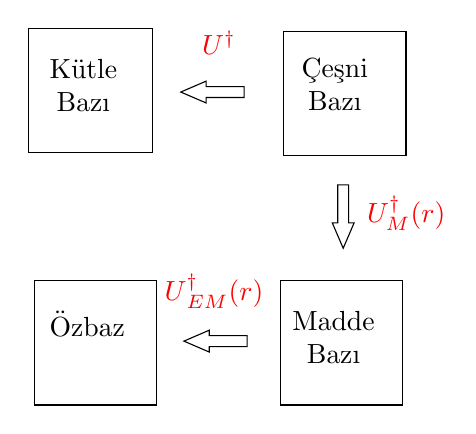
\begin{tikzpicture}[x=0.75pt,y=0.75pt,yscale=-1.5,xscale=1.5]
  %uncomment if require: \path (0,300); %set diagram left start at 0, and has height of 300

  %Shape: Rectangle [id:dp8088308900717263] 
  %\draw   (31,101) -- (70.33,101) -- (70.33,141) -- (31,141) -- cycle ;
  \draw   (30,100) -- (70,100) -- (70,140) -- (30,140) -- cycle ;
  %Right Arrow [id:dp5637298668216818]
  %\draw   (99.33,122.25) -- (87.13,122.25) -- (87.13,124) -- (79,120.5) -- (87.13,117) -- (87.13,118.75) -- (99.33,118.75) -- cycle ;
  \draw   (99.33,122.25) -- (87.13,122.25) -- (87.13,124) -- (79,120.5) -- (87.13,117) -- (87.13,118.75) -- (99.33,118.75) -- cycle ;
  %Shape: Rectangle [id:dp5085257977019034] 
  \draw   (112,101) -- (151.33,101) -- (151.33,141) -- (112,141) -- cycle ;
  %Shape: Rectangle [id:dp33001506333160935] 
  \draw   (111,181) -- (150.33,181) -- (150.33,221) -- (111,221) -- cycle ;
  %Right Arrow [id:dp5718992848093374] 
  \draw   (132.92,150.33) -- (132.92,162.53) -- (134.67,162.53) -- (131.17,170.67) -- (127.67,162.53) -- (129.42,162.53) -- (129.42,150.33) -- cycle ;
  %Right Arrow [id:dp6931270939254744] 
  \draw   (100.33,202.25) -- (88.13,202.25) -- (88.13,204) -- (80,200.5) -- (88.13,197) -- (88.13,198.75) -- (100.33,198.75) -- cycle ;
  %Shape: Rectangle [id:dp069718532513661] 
  \draw   (32,181) -- (71.33,181) -- (71.33,221) -- (32,221) -- cycle ;

    % Text Node
  \draw (138,153) node [anchor=north west][inner sep=0.75pt]  {$\textcolor[rgb]{1,0,0}{U_{M}^{\dagger }( r)}$};                                     
  % Text Node                                                                                                                                                           
  \draw (73,178) node [anchor=north west][inner sep=0.75pt]  {$\textcolor[rgb]{1,0,0}{U}\textcolor[rgb]{1,0,0}{_{EM}^{\dagger }}\textcolor[rgb]{1,0,0}{(}\textcolor[rgb]{1,0,0}{r}\textcolor[rgb]{1,0,0}{)}$};                                                                                                                    
  % Text Node                                                                                                                                                           
  \draw (85,100) node [anchor=north west][inner sep=0.75pt] {$\textcolor[rgb]{1,0,0}{U^{\dagger }}$};                                              
  % Text Node                                                                                                                                                           
  \draw (36,109) node [anchor=north west][inner sep=0.75pt] [align=center] {{Kütle}\\{Bazı}};                                
  % Text Node                                                                                                                                                           
  \draw (117,109) node [anchor=north west][inner sep=0.75pt] [align=center] {{Çeşni}\\{Bazı}};                             
  % Text Node                                                                                                                                                           
  \draw (114,190) node [anchor=north west][inner sep=0.75pt]  [align=center] {{Madde}\\{Bazı}};                             
  % Text Node                                                                                                                                                           
  \draw (36,190) node [anchor=north west][inner sep=0.75pt] [align=center] {{Özbaz}};                              
\end{tikzpicture}
	\caption[Bazlar arası dönüşüm diyagramı.]{Bazlar arası dönüşüm diyagramı.}
	\label{fig:transfDiagram}
\end{figure}

\subsubsection{ANALİTİK ÇÖZÜLEBİLEN ÖZEL DURUMLAR}
\paragraph{}
İkinci ve üçüncü çözüm yöntemlerine geçmeden önce \eqref{eqn:HamiltonyenToplam} numaralı bağıntıda verilen toplam Hamiltonyen'i $ 2\times2 $ matrise indirgememiz gerekmektedir. Bu indirgeme işlemi ile $ \Delta s_{2\theta} $ terimini ihmal ediyoruz. Bu yaklaşıklık, boşluk karışım açısı $ \theta $'nın, küçük değerleri için uygun bir yaklaşımdır. Hamiltonyen'in elektromanyetik etkileşimler dikkate alınarak indirgenmesi iki farklı şekilde olabilir. Birincisi $ e-\bar{x} $ terimlerini alarak, buna $ H_{T,e\bar{x}} $ adı verilecektir, veya $ x-\bar{e} $ terimleri alarak, buna da $ H_{T,x\bar{e}} $ adı verilecektir, indirgeyebiliriz.
\begin{align}
	\label{eqn:Hamiltonyen_T14}H_{T,e\bar{x}} &= \mqty(-\Delta c_{2\theta}+V_{CC}+V_{NC} & \mu B \\ \mu B & \Delta c_{2\theta}-V_{NC}) \\
	\label{eqn:Hamiltonyen_T23}H_{T,x\bar{e}} &= \mqty(\Delta c_{2\theta}+V_{NC} & -\mu B \\ -\mu B & -\Delta c_{2\theta}-V_{CC}-V_{NC})
\end{align}
Hamiltonyen'i $ e-\bar{x} $ ve $ x-\bar{e} $ olarak ayırmamızın sebebi nötrino antinötrino geçişlerinin ancak ve ancak $ e-\bar{x} $ ve $ x-\bar{e} $ arasında olmasıdır. Hamiltonyen'in $ \dyad{\nu_{e}}{\nu_{\bar{e}}} $ ve $ \dyad{\nu_{x}}{\nu_{\bar{x}}} $ bileşenleri sıfırdır. Hangi matrisin ne zaman kullanılması gerektiği ise \ref{sec:sfpRezonansi} numaralı kısımda açıklanacaktır.

Hamiltonyen'i \eqref{eqn:NuKim_EoM_4Mat} numaralı denklemde yerine koyacağız. \eqref{eqn:NuKim_EoM_4Mat} numaralı denklemdeki çeşniler düzeltildikten sonra Hamiltonyenler'in $ ee $ elemanları sıfır olacak şekilde birim matrisle orantılı terimler çıkaracağız.
\begin{align}
	\label{eqn:EoM_14Matris}i\dv{}{r} \mqty(\ket{\nu_{e}} \\ \ket{\nu_{\bar{x}}}) &= 
	\mqty(0 & \mu B \\ \mu B & 2\Delta c_{2\theta}-V_{CC}-2V_{NC}    ) 
	\mqty(\ket{\nu_{e}}\\ \ket{\nu_{\bar{x}}}) \text{ ,}\\
	\label{eqn:EoM_23Matris}i\dv{}{r} \mqty(\ket{\nu_{x}} \\ \ket{\nu_{\bar{e}}}) &= 
	\mqty(0 & -\mu B \\ -\mu B & -2\Delta c_{2\theta}-V_{CC}-2V_{NC} ) 
	\mqty(\ket{\nu_{x}}\\ \ket{\nu_{\bar{e}}}) \text{ .}
\end{align}

Nötrino hareket denklemleri birinci dereceden çiftlenmiş (coupled) diferansiyel denklemlerdir. İki adet birinci dereceden hareket denklemleri, bir adet ikinci dereceden hareket denklemi haline getirilebilir. Basitlik olması açısından $ \nu_{1} \equiv \ket{\nu_{e}} $ ve $ \nu_{2} \equiv \ket{\nu_{x}} $ olarak değiştirilecektir (bu isimlendirme ile kütle tabanını karıştırmayınız.) Bu değişikliklerden sonra $ \nu_{1} $, \eqref{eqn:EoM_14Matris} numaralı denklemin çözümü ve $ \nu_{2} $ ise \eqref{eqn:EoM_23Matris} numaralı denklemin çözümü olacaktır.
\begin{equation}
	\dv[2]{\nu_{i}}{r} + \left(i\kappa_{i}+iP(r) + \frac{\dv{B}{r}}{B(r)}\right) 
    ~\dv{\nu_{i}}{r}+ (\mu B(r))^{2}~ \nu_{i} = 0 \text{ .}
\end{equation}
Burada $ P(r) \equiv -\sqrt{2}G_{F}(1-2Y_{e})N_{b}(r) $ ve $ \kappa_{1,2} \equiv \mp 2\Delta c_{2\theta} $ şeklinde tanımlanmıştır (bu isimlendirme ile olasılık hesabındaki ifadeyi karıştırmayınız.) Bu denklemler çok kullanılan baryon ve manyetik alan profilleri için çözülememektedir. Örneğin, manyetik alanın polinom tipi bir profile, baryon yoğunluğunun eksponansiyel profile sahip olduğu durumda bir çözüm yoktur. En genel çözümü bulmaktansa bu bölümde \emph{sabit manyetik alan} ve \emph{eksponansiyel olarak aynı şekilde azalan baryon ve manyetik alan} profillerini kullanacağız. Hareket denkleminin genel hali aşağıdaki gibi olur.
\begin{equation}\label{eqn:app_diffeqConstB}
    \dv[2]{\nu_{i}}{r} + i\left(\kappa_{i}+P(r)\right) ~\dv{\nu_{i}}{r}+ 
    (\mu B(r))^{2}~ \nu_{i} = 0 \text{ .}
\end{equation}
Bu tip denklemlere \emph{konfluent hipergeometrik} denklemler adı verilir. Denklemlerin bu formu, sadece madde etkileşimi dikkate alındığında da karşımıza çıkar. Sadece madde etkileşimi aldığımız durumda, köşegen olmayan terim $ \mu B $ yerine $ \Delta s_{2\theta} $ ve köşegen terim ise $ \kappa_{i} + P(r) \equiv 2\Delta c_{2\theta} - V_{CC} $ şeklinde gelecektir. Sadece madde etkileşiminde çeşitli baryon (veya elektron) profillerine göre elde edilen çözümler \cite{Ito:1987vy,Toshev:1987jw,Kaneko:1987zza, Notzold:1987cq, Kuo:1989qe,Balantekin:1996ag} numaralı referanslarda verilmiştir. Bu eşdeğerlilik, $ B $'nin uzaklığa bağlı olduğu durumlarda kırılır. 

Sabit dış manyetik alan profili için çözümler \emph{Kummer Fonksiyonları} cinsinden yazılır. Burada,baryon profili $ N_{b}(r) = N_{i}\exp(-\alpha r) $ ve elektron kesri $ Y_{e} $ sabit olacak şekilde madde potansiyeli seçilmiştir. Dikkate alınan bu profillerin ışığında \eqref{eqn:app_diffeqConstB} numaralı denklemlerin çözümleri aşağıdaki gibi olur.
\begin{align}
    \nonumber \nu_{i}(r) & = N_{1}^{\xi^{+}_{i}}~ _{1}F_{1}\left(\xi^{+}_{i}; 
    1+2\xi^{+}_{i}-\kappa_{i};\frac{-iP(r)}{\alpha} \right) \\
    & + N_{2}^{\xi^{-}_{i}} ~ _{1}F_{1}\left(\xi^{-}_{i}; 1+2\xi^{-}_{i}-
    \kappa_{i};\frac{-iP(r)}{\alpha}\right) \text{ ,}
\end{align}
Burada $N_{1,2} \equiv C_{1,2}\frac{i}{\alpha} (\pm \sqrt{2}G_{F}(2Y_{e}-1)n_{i}e^{-\alpha r} )$ ve
\begin{equation}
  \xi^{\mp}_{i} \equiv \frac{i(\kappa_{i} \mp \sqrt{(2\mu B)^{2} + 
  \kappa^{2}_{i} } )}{2\alpha} \text{ ,}
\end{equation}
şeklindedir. Kummer'in fonksiyonları, $ _{1}F_{1}(a;b;z) $, konfluent hipergeometrik denkleminin çözümleridir. $ C_{1,2} $ katsayıları ise çözümlerin limit durumlarından çıkarılır. Örneğin, $ B \rightarrow 0 $ limitinde çeşniler arası salınım olmaması gerekmektedir. Bu ve bunun gibi limitler kullanılarak integral sabitleri belirlenir.

Çözümü olan bir diğer profil ise manyetik alanın ve baryon yoğunluğunun aynı eksponansiyel fonksiyona sahip olduğu durumdur; elektron kesri sabittir. Bu profiller kullanıldığında hareket denklemi aşağıdaki gibi olur.
\begin{equation}\label{eqn:app_exactdiffeqSameAlpha}
    \dv[2]{\nu_{i}}{r} + \left(i\kappa_{i}+iP(r) + \alpha\right)
    \dv{\nu_{i}}{r}+ (\mu B_{i}e^{-\alpha r})^{2}~ \nu_{i} = 0 \text{ .}
\end{equation}
Burada baryon yoğunluğu ve manyetik alan $ \exp(-\alpha r) $ şeklinde uzaklığa bağlıdır. $ B_{i} $ ise başlangıç noktasındaki manyetik alanın büyüklüğüdür. \eqref{eqn:app_exactdiffeqSameAlpha} numaralı denklemin çözümü genelleştirilmiş hipergeometrik fonksiyonlar $ U(a,b,z) $ ve birleşmiş Laguerre polinomları (associated Laguerre polynomials) $ L(n,l,m) $ cinsinden verilir. Açık ifadeleri bu tezin kapsamı dışındadır. Yaklaşık çözümler için \cite{Balantekin:2004tk} numaralı kaynağa ve Demkov-Kunike modeli için \cite{Joshi:2019dcj} numaralı kaynağa bakınız.

\subsubsection{ADYABATİK EVRİM ÇÖZÜMLERİ}
\paragraph{}
Toplam Hamiltonyen \eqref{eqn:HamiltonyenToplam} numaralı denklemin üçüncü ve son çözüm yöntemi ise efektif karışım açısı elde etmektir. Efektif karışım açısının elde edilmesi ile \ref{subsec:MaddeOrtamindaNuEvrimi} numaralı bölümde $ \barparen{\theta}_{M} $ elde edilmesi benzerlik gösterir. Bunun için \eqref{eqn:Hamiltonyen_T14} ve \eqref{eqn:Hamiltonyen_T23} numaralı denklemlerde verilen Hamiltonyenler'i köşegenleştiren dönme (dönüşüm) matrislerini elde etmek gerekecektir. Köşegenleştirme Bloch vektörü yardımıyla yapılacaktır.

$ H_{T,e\bar{x}} $ Hamiltonyen'i için yazılacak olan Bloch vektörü $ \vec{B}_{T,e\bar{x}} $ ve $ H_{T,x\bar{e}} $ için yazılacak olan Bloch vektörü $ \vec{B}_{T,x\bar{e}} $ olarak adlandırılacaktır.
\begin{align}
	\vec{B}_{T,e\bar{x}} =& \mqty(2\mu B & 0 & 2 \Delta c_{2\theta} - V_{CC}-2V_{NC})_{\text{çeşni}} \text{ ,}\\ \vec{B}_{T,x\bar{e}} =& \mqty(2\mu B & 0 & -2 \Delta c_{2\theta} - V_{CC}-2V_{NC})_{\text{çeşni}} \text{.}
\end{align}
Buradan özdeğerler,
\begin{align}
	\label{eqn:Ozdeger_EMetkilesim14}(\lambda_{1,2})_{e\bar{x}} =& \pm M_{EM} + V_{CC}/2 \text{ ,} \\
	\label{eqn:Ozdeger_EMetkilesim23}(\lambda_{1,2})_{x\bar{e}} =& \pm \overline{M}_{EM} - V_{CC}/2
\end{align}
şeklinde yazılır. Burada $ \barparenBig{M}_{EM} = \sqrt{(\mu B)^{2} + (\Delta c_{2\theta} \pm V_{NC} \pm V_{CC}/2)^{2}} $ şeklindedir Özvektörleri veren efektif elektromanyetik karışım açıları ise 
\begin{equation}\label{eqn:theta_EM_hepsi}
	\tan 2\barparen{\theta}_{EM} = \frac{\mu B}{\Delta c_{2\theta} \pm V_{NC} \pm V_{CC}/2} \text{ ,}
\end{equation}
şeklinde yazılır. Madde etkileşiminde elde edilen, $ \theta_{M}(r) $ açısı kullanılarak yazılan $ U_{M}(r) $ dönüşüm matrisi, $ \theta_{EM}(r) $ kullanılarak da da yazılır. Bu yöntem ile elde edilen $ U_{EM}(r) $ matrisi ile \eqref{eqn:U_EM_tedirgenmis} numaralı denklemde verilen $ U_{EM}(r) $ matrisi farklıdır. \eqref{eqn:U_EM_tedirgenmis} numaralı denklemdeki dönüşüm dört çeşni, düşük manyetik alan yaklaşıklığında elde edilmiş, \eqref{eqn:theta_EM_hepsi} numaralı denklemdeki dönüşüm matrisi ise iki çeşni ve düşük $ \Delta s_{2\theta} $ yaklaşıklığında üretilmiştir. Aksi belirtilmedikçe $ \theta_{EM}(r) $ açısından elde edilen dönüşüm matrisi kullanılacaktır.
	
Hamiltonyen'i indirgeyerek elde edilen fiziksel büyüklükler, Hamiltonyen'in $ ex $, $ e\bar{e} $ ve $ x\bar{x} $ terimleri dikkate alınarak da yapılır. Bu işlemleri ayrı ayrı yapmak yerine genelleştirilmiş ifadesini elde etmek mümkündür. \cite{Likhachev:1990ki,Broggini:2012df}. Not edilmelidir ki, birazdan yazılacak olan genelleştirmelerin hepsi alt matrise indirgendikten sonra hesaplanır. Örneğin, $ \alpha=e $ ve $ \beta=\bar{x} $ alındığında \eqref{eqn:EoM_14Matris} numaralı Hamiltonyen ile alakalı büyüklükler elde edilir. $ H_{\alpha\beta} $, \eqref{eqn:HamiltonyenToplam} numaralı Hamiltonyen'in elemanları olmak üzere yaşama olasılığı \cite{Giunti:2014ixa}
\begin{equation}
	P_{\nu_{\alpha} \rightarrow \nu_{\alpha}} = 1 - \sin^{2} 2\theta_{EM} \sin^{2}(\frac{\pi}{L_{EM}}r) \text{ ,}
\end{equation}
şeklinde yazılır. Bu ifade başlangıçta sadece $ \alpha $ çeşnisine sahip nötrinoların yaşama olasılıklarını veren genel ifadedir. Efektif açı $ \theta_{EM} $ yerine $ \theta $ konulduğunda boşlukta ilerleyen $ \alpha $ nötrinolarının yaşama olasılıklarını verir. Bu denklemdeki $ L_{EM} $ salınım dalga boyudur ve aşağıdaki gibi genel olarak tanımlanabilir.
\begin{equation}
	L_{EM}= \frac{2\pi}{\sqrt{4_{H_{\alpha\beta}}^2+(H_{\beta\beta} - H_{\alpha\alpha})^{2}}} \text{ .}
\end{equation}

Hamiltonyen'in elemanlarından salınım dalga boyunu yazabileceğimiz gibi karışım açısı $ \theta_{EM} $ terimini de yazabiliriz. Burada $ \theta_{EM} $ açısının tanjantı değil $ \theta_{EM} $ açısının sinüsünün yazıldığına dikkat edilmelidir \footnote[1]{\cite{Broggini:2012df} numaralı kaynakta efektif açı $ \theta_{EM} $ olarak tanımlanmış ancak \cite{Likhachev:1990ki} numaralı kaynakta $ 2\theta_{EM} $ olarak tanımlanmıştır.}.
\begin{equation}
	\sin 2\theta_{EM} = \frac{H_{\alpha\beta}}{\sqrt{H^{2}_{\alpha\beta} + \qty[(H_{\beta\beta} - H_{\alpha\alpha})/2]^{2}}} \text{ .}
\end{equation}

\eqref{eqn:theta_EM_hepsi} numaralı denklemde verilen efektif karışım açılarını yukarıdaki formülden de elde etmek mümkündür. Hamiltonyen'in $ e\bar{x} $ elemanı için ($ \theta_{EM} $), $ (\alpha,\beta)=(1,4) $ ikilisi ve Hamiltonyen'in $ x\bar{e} $ elemanı için ($ \bar{\theta}_{EM} $), $ (\alpha,\beta)=(2,3) $ ikilisi seçilmelidir.

Efektif elektromanyetik karışım açısının tanjantını \eqref{eqn:theta_EM_hepsi} numaralı denklemde elde etmiştik. \eqref{eqn:V_NC} ve \eqref{eqn:V_CC} numaralı denklemlerdeki madde etkileşim potansiyellerinin ($ V_{CC} $ ve $ V_{NC} $) açık ifadeleri kullanılarak da yazabiliriz. 
\begin{align}
	\tan 2\barparen{\theta}_{EM} = \frac{\mu B}{\Delta c_{2\theta} \pm (\sqrt{2}G_{F}N_{b})(2Y_{e}-1)/2} \text{ .}
\end{align}
Bu açık ifadeleri kullandığımızda, $ Y_{e}=0.5 $'in özel bir değer olduğu görülür. Bu özel değerde, efektif karışım açısı aşağıdaki gibi verilir.
\begin{equation}
	\eval{\tan 2\barparen{\theta}_{EM}}_{Y_{e}=0.5} = \frac{\mu B}{\Delta c_{2\theta}} \text{.}
\end{equation}

$ Y_{e}=0.5 $ değeri için efektif elektromanyetik karışım açısı içerisinde madde etkileşim terimi bulunmamaktadır. Bu limitte Hamiltonyen'i $ 2\times2 $ boyutlu matrise indirgerken dikkatli olunması gerekmektedir. $ Y_{e}=0.5 $ limitinde \eqref{eqn:EoM_14Matris} ve \eqref{eqn:EoM_23Matris} numaralı Hamiltonyenler'i tekrar yazalım.
\begin{align}
	\label{eqn:EoM_14MatrisYe05}\eval{H_{T,e\bar{x}}}_{Y_e=0.5} &= 
	\mqty(0 & \mu B \\ \mu B & 2\Delta c_{2\theta}) \text{ ,}\\
	\label{eqn:EoM_23MatrisYe05}\eval{H_{T,x\bar{e}}}_{Y_e=0.5}&= 
	\mqty(0 & -\mu B \\ -\mu B & -2\Delta c_{2\theta}) \text{ .}
\end{align}
Yukarıdaki yazılan iki matris de aynıdır. Hamiltonyen'i indirgerken boşluk salınımlarının etkisinin çok düşük olacağı varsayılmıştı. $ Y_{e}=0.5 $ limitinde bu varsayım, sadece ve sadece $ \mu B \gg 2\Delta c_{2\theta}$ yaklaşıklığında geçerli olacaktır. %Madde etkileri gittiğinde $ \Delta s_{2\theta} $ terimini sadece $ \mu B $ ile kıyaslayarak ihmal edebiliriz.

Son olarak bu limitte özdeğerler de yazılabilir. Özdeğerler her iki Hamiltonyen için aynı olacaktır.
\begin{equation}\label{eqn:eigValTotal_Ye05}
	\eval{(\lambda_{1,2})}_{Y_{e}=0.5} = \pm\sqrt{(\mu B)^{2} + (\Delta c_{2 \theta})^{2}}\text{ .}
\end{equation}
Dikkatli bakıldığında $ \theta = 0 $ için \eqref{eqn:eigValTotal_Ye05} ve \eqref{eqn:eigValNuEm} numaralı denklemler aynıdır. 

Sonuç olarak nötrino elektromanyetik alan etkileşimini ve nötrino madde etkileşimini dikkatte aldığımızda, $ Y_{e}=0.5 $ için madde etkileri neredeyse yok olmaktadır. Bu limit astrofiziksel ortamlar için önemlidir, çünkü $ Y_{e}=0.5 $, nötr bir ortam için proton ve nötron sayılarının eşitliği anlamına gelir.

Bir sonraki bölümde nötrino-nötrino etkileşimlerinden kaynaklanan terimler incelenecektir. Astrofiziksel ortamlarda yani nötrino yoğunluğunun çok yüksek olduğu yerlerde nötrino-nötrino etkileşimlerinden bahsetmek mümkün olacaktır.

\section{NÖTRİNO ÖZ-KIRILIMI}\label{sec:notrinoOzKirilimi} % Self-Refraction

Nötrinoların Standart Model etkileşim tesir kesitleri diğer temel parçacıklara nazaran çok küçüktür \cite{Formaggio:2012cpf}. Buna rağmen ÇÇSN, nötron yıldızı birleşmeleri veya kozmoloji gibi nötrino akısının (flux) çok yüksek olduğu fenomenlerde nötrino - nötrino etkileşimleri söz konusu olabilir \cite{Berryman:2022hds}. Nötrino - nötrino etkileşmelerinin efektif Hamiltonyen'i diğer etkileşimler gibi değildir ve ortamın geometrisine bağlıdır. Bu bölümde nötrino - nötrino etkileşimlerini inceleyeceğiz. Literatürde nötrino - nötrino etkileşimleri ismi yerine nötrino öz-etkileşimi \cite{Berryman:2022hds} (self-interaction), nötrino öz-kırılımı (self-refraction) \cite{Pehlivan:2010zz,Friedland:2010sc}, nötrino kolektif çeşni değişimi \cite{Chakraborty:2016yeg} gibi isimler kullanılmaktadır. Tezin geri kalanında nötrino - nötrino etkileşimleri yerine nötrino öz-kırılımı ifadesi kullanılacaktır.

Nötrino madde etkileşimlerinden ve nötrino elektromanyetik etkileşimlerden farklı olarak nötrino öz-kırılımı dinamik bir etkileşimdir. Nötrinolar arka plandaki madde veya manyetik alanla etkileşirken, etkileşilen madde ve manyetik alanın değişmediği varsayılmıştır. Bu durum etkileşimleri statik yapar. Nötrino öz-kırılımında ise test nötrinosu, diğer nötrinoların oluşturduğu nötrino alanı ile etkileşir. Bu etkileşimin hemen ardından nötrinoların tüm çeşni yapısı değişecektir. Bunun sonucunda arka plandaki nötrino profili her adımda değişecektir. Bu nedenden ötürü nötrino öz-kırılma Hamiltonyen'i içerisinde nötrino alanının integrali bulunmaktadır. Aynı zamanda bu dinamik değişim hareket denklemlerini de birbirine bağlar. Çeşni evrimini veren \eqref{eqn:NuKim_LiouvilleVonNeumann} numaralı denklem seti birbirine bağlı yani çiftlenmiş (coupled) olacaktır. Buna ek olarak, nötrino profilinin dinamik olması, \eqref{eqn:NuKim_LiouvilleVonNeumann} numaralı denklem setini doğrusal olmayan (non linear) diferansiyel denklem haline getirecektir.

Nötrino öz-kırılım Hamiltonyen'i aşağıdaki gibi yazılır \cite{Sigl:1993ctk}.
\begin{align}\label{eqn:Hamil_nunuOperator}
	\nonumber \hat{H}_{\nu\nu}(r)= & \sum_{\alpha\beta=e,x,\bar{e},\bar{x}} (H_{\nu\nu})_{\alpha\beta} \dyad{\nu_{\alpha}}{\nu_{\beta}} \text{ ,}\\ 
	=&\sqrt{2} G_{F} D(r)\sum_{\alpha,\beta = e,x} \qty[\int \qty[\rho_{\alpha\beta}(E,r)-\rho_{\bar{\alpha}\bar{\beta}}(E,r)]\dd{E}] \qty(\dyad{\nu_{\alpha}}{\nu_{\beta}}-\dyad{\nu_{\bar{\alpha}}}{\nu_{\bar{\beta}}}) \text{ .}
\end{align}
Burada $ D(r) $, sistemin geometrisinden gelen katkıdır ve \ref{subsec:geometri} numaralı bölümde tartışılacaktır. Öz-kırılım Hamiltonyen operatörü Standart Model çiflenim sabitine göre yazılmıştır. Bu operatör çeşni tabanında yazılmıştır, ancak öz-kırılım Hamiltonyen'i tabandan bağımsızdır. Yani üniter dönüşümler altında değişmez (invariant) kalır. Matris temsili $ (H_{\nu\nu})_{\alpha\beta} $ ise

{\small
\begin{equation}
	(H_{\nu\nu})_{\alpha\beta}(r) = \sqrt{2} G_{F} D(r) \int \dd{E} \mqty((\rho_{ee}-\rho_{\bar{e}\bar{e}}) & (\rho_{ex}-\rho_{\bar{e}\bar{x}}) & 0 & 0\\ (\rho_{xe}-\rho_{\bar{x}\bar{e}}) & (\rho_{xx}-\rho_{\bar{x}\bar{x}}) & 0 & 0\\ 0 & 0 & (\rho_{\bar{e}\bar{e}} -\rho_{ee}) & (\rho_{\bar{e}\bar{x}} -\rho_{ex}) \\ 0 & 0 & (\rho_{\bar{x}\bar{e}} -\rho_{xe}) & (\rho_{\bar{x}\bar{x}} -\rho_{xx})) \text{ ,}
\end{equation}}
şeklinde yazılır. Hamiltonyen matrisine bakıldığında nötrino - antinötrino geçişleri bulunmamaktadır. Öz-kırılım Hamiltonyen'i sadece ileri saçılmaları (forward scattering) dikkate almıştır. İleri saçılmalar, öz-kırılım Hamiltonyen'ine en büyük katkıyı getirecektir \cite{Cherry:2013mv, Volpe:2015rla}

Nötrino öz-kırılımının çeşni evrimine etkisi ele alınan sistemin geometrisine göre çeşitlilik gösterir. Örneğin, küresel bir kaynaktan çıkan nötrinolar için etkileşim geometrisi küresel simetrik olur. Ortamda var olan nötrinolar belli bir açıyla öz-kırılım potansiyelinin içerisine girer ve birbirleri ile etkileşirler. Bu geometriye örnek olarak ÇÇSN gösterilebilir. Bir diğer taraftan iki nötron yıldızının birleşmesi gibi iki kaynaktan çıkan nötrinoların oluşturduğu geometri daha karmaşıktır. Bu tezde nötrinoların ÇÇSN'nın merkezinde oluşan proto-nötron yıldızından çıktığı varsayılacaktır. Öz-kırılım geometrisi ise \ref{subsec:geometri} numaralı bölümde ayrıntılı olarak ele alınmıştı.

Nötrino öz-kırılımı için efektif karışım açısı veya Bloch vektörü yazmak olanaksızdır, çünkü çözülecek olan hareket denklemi yoğunluk matrisinin kendisine bağlıdır. Bu nedenle, öz-kırılım Hamiltonyen'i dikkate alındığında hareket denklemlerinin analitik çözümü bulunmamaktadır. Buna rağmen iki çeşni için çeşitli simetriler ve değişmezler (invariants), yani korunan büyüklükler hesaplanabilir \cite{Pehlivan:2011hp}. Simetriler ve korunan büyüklükler bu tezde bahsedilmeyecek olan polarizasyon vektörü ve özellikleri kullanılarak hesaplanır \cite{fackler1986Massive}. Analitik çözümün eğilimini belirlemek adına hareket denklemini doğrusallaştırılıp (linearization) incelemek de literatürde kullanılan bir yöntemdir. Bu doğrusallaştırma neticesinde çeşitli analizler yapılabilir \cite{Chakraborty:2014lsa, Chakraborty:2019wxe, Xiong:2021dex}. Çeşitli sayısal çözümler ve spektral ayrışma/ spektral yer değiştirme (spectral split/spectral swap) gibi kolektif etkiler \ref{ch:simulasyonlar} numaralı bölümde ayrıntılı olarak ele alınacaktır.
\newpage
\chapter{REZONANSLAR}\label{ch:Rezonanslar}
Rezonans olayını anlamak için Hamiltonyen'in matris formülasyonu daha uygundur. İki seviyeli bir sistem için gerçel bir Hamiltonyen aşağıdaki gibi yazılabilir.
\begin{equation}
	H = \mqty(0 & H_{12}\\ H_{12} & H_{22} ) \text{ .}
\end{equation}

Rezonans olayını anlayabilmek için sistemi basitleştirelim. Başlangıçtaki durum keti $ \ket{\Psi(R)} = \mqty(1 & 0)^{T} $ olsun, yani başlangıçta sadece elektron nötrinosu olsun. Elektron nötrinosundan x nötrinosuna geçişi $ H_{12} $ elemanı kontrol edecektir. $ H_{12} $ elemanı evrim boyunca sıfır veya sıfıra yakın olduğunda sistem başlangıçtaki özdurumundan sapmayacaktır ve elektron nötrinosu olarak hayatına devam edecektir. Bir diğer taraftan Hamiltonyen'in köşegen terimi $ H_{22} $, $ H_{12} $'ye göre küçük ise sistem başlangıçtaki durumunda olmayacak, iki özdurumun bir süperpoziyonu olacaktır. Herhangi bir $ r $ uzaklığında nötrino çeşni ölçümü yapıldığında x nötrinosu olma olasılığı sıfırdan farklı olacaktır.

Rezonans etkisi, evrimin bir aşamasında $ H_{11}-H_{22} $ farkının sıfır olduğunda ve $ H_{12} $ elemanının sıfırdan farklı olduğu durumda ortaya çıkacaktır. Bu durumda köşegen elemanlar sıfır olacak ve karışım maksimum olacaktır. Bunun anlamı tüm elektron nötrinolarının x nötrinosuna geçmesidir.

Rezonans etkisini genel olarak anlayabilmek için sistemin özdeğerlerine bakmak gerekecektir. Özdeğerlere karşılık gelen özvektörler takip edilerek rezonans durumu incelenebilir. Bunun için özdeğerlerin konuma bağlı değişimi bakılır. Özdeğerler önce birbirlerine yakınlaşır sonra uzaklaşırsa sistem rezonansa girmiş demektir. Bizim ilgilendiğimiz sistemlerde özdeğerler birbirlerine yakınlaşacak ve sistem rezonanslara girecektir.

Rezonans bölgesinde özdurumların birbirlerine \emph{zıplamasının} ifadesini veren Landau - Zener geçiş olasılıklarını hesaplamadan önce Zener'in makalesinde \cite{1932RSPSA.137..696Z} yapılan yaklaşıklıklar açıklanacaktır. 
\begin{enumerate}
	\item Hamiltonyen'in geçişten sorumlu olan elemanı (yukarıdaki basit örnekte $ H_{12} $) konumdan bağımsız olmalıdır.
 	\item Başlangıçtaki anlık (instantaneous) özdurumlar, başlangıç durumu ile aynı olmalıdır. Örneğin başlangıçta sadece elektron nötrinosu var ise sistemin başlangıçtaki özdurumu da çeşni tabanı olmalıdır. Bu yaklaşıklık, Hamiltonyen'deki çeşni geçişinden sorumlu olan elemanının, başlangıçta küçük olmasını zorunlu kılar.
  	\item Özdeğerlerin yakınlaştığı geçiş bölgesinde özdeğer farkları doğrusal olmalıdır.
\end{enumerate}

İki seviyeli sistemlerde LZ geçiş olasılığını bulmak için en genel Hamiltonyen'i yazacağız \cite{1981PhRvA..23.3107R}.
\begin{equation}
	H(r) = \mqty(\omega_{1}(r) & \frac{1}{2} \omega_{0} e^{-i\phi}\\ \frac{1}{2} \omega_{0} e^{i\phi} & \omega_{2}(r) ) \text{ .}
\end{equation}
Burada $ \omega_{0} $, birinci yaklaşıklıktan dolayı konumla değişmemektedir. Bizim kullanacağımız Hamiltonyenler gerçel olduğu için sanal $ \phi $ fazını sıfır alacağız. Bunlara ek olarak çoğunlukla izsiz Hamiltonyenler ile çalışacağımız için $ \omega_{1}+\omega_{2} $ terimi de sıfır olacaktır. 

Bu Hamiltonyen'in özdeğerleri, 
\begin{equation}
	\omega_{a,b} = \frac{1}{2} \pm \sqrt{\qty(\omega_{1}(r)-\omega_{2}(r))^{2}+ \omega_{0}^{2}} \text{ ,}
\end{equation}
şeklinde yazılır. Eğer Hamiltonyen'in köşegen olmayan terimi sıfır olursa, özdeğerler çakışabilir. Böyle bir durumda, özdeğerlerin çakıştığı noktanın özel bir anlamı yoktur. Eğer köşegen olmayan terim sıfır olmaz ise özdeğerler, çakışma noktası etrafında birbirlerinden uzaklaşacaktır.

Kaçınan kesişme (avoided crossing), özdeğerlerin birbirlerine yaklaşması ve ardından ayrılması olarak karakterize edilir. Özdeğerlerin yakınlaşması \ref{fig:avoidCrossing} numaralı şekilde gösterilmiştir. Bu şekilde birbirlerine en yakın olunan nokta $ q_{c} $ noktasıdır. $ q $, Hamiltonyen'i parametrize eden değişkendir. Bizim ilgileneceğimiz sistemler konuma göre evrilecektir. Bundan dolayı kritik nokta $ q_{c} $, kritik uzaklık $ r_{c} $ olacaktır. Kritik noktanın diğer noktalardan ayrılan özelliği, evrim boyunca özdeğerlerin birbirine en yakın olduğu nokta olmasıdır. İşte bu noktada da rezonans meydana gelmektedir. $ \omega_{a}-\omega_{b} $ ise geçişin genişliğini, $ \omega_{0} $ ise özdeğerlerin ne oranda açıldığını karakterize eder. Eğer $ \omega_{0}/\dv{(\omega_{a}-\omega_{b})}{r} $ küçük ise durumlar arası geçiş diyabatiktir, tersi ise adyabatiktir.
\begin{figure}[hbt!]
	\centering
	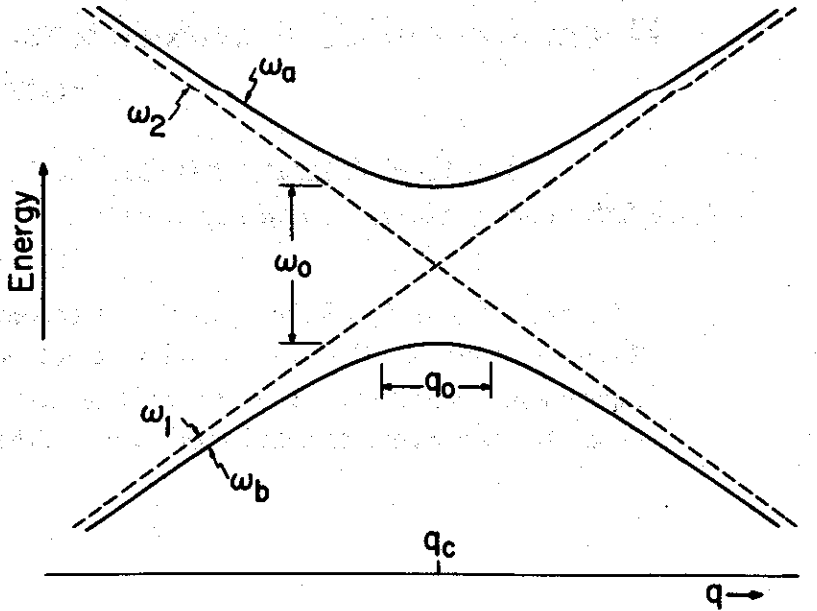
\includegraphics[width=0.5\textwidth]{figures/Avoid_Crossing_With_Paramters.png}
	\caption[Özdeğerlerin Kaçınan Kesişmeleri]{Özdeğerlerin Kaçınan Kesişmeleri. Bu grafik \cite{1981PhRvA..23.3107R} numaralı kaynaktan alınmıştır.}
	\label{fig:avoidCrossing}
\end{figure}

Geçiş olasılığını verecek olan $ \Gamma $ parametresi yani \emph{adyabatisite parametresi} aşağıdaki gibi tanımlanır.
\begin{equation} \label{eqn:LZ_Gamma_def}
	\Gamma = \eval{\frac{\omega^{2}_{0}}{4 \dv{r} \qty[\omega_{1}(r)-\omega_{2}(r)]}}_{r=r_{c}} \text{ .}
\end{equation}
Burada $ \Gamma $ parametresi hesaplanırken, türev alındıktan sonra uzaklık yerine rezonansın uzaklığı yani kritik uzaklık $ r_{c} $ konulmalıdır. Geçiş olasılığını elde etmek için $ r_{\text{başlangıç}} \rightarrow -\infty $ ve $ r_{\text{bitiş}} \rightarrow \infty $ limiti alınırsa sonuç 
\begin{equation}\label{eqn:LZOlasilik}
	P = e^{-2\pi \Gamma}
\end{equation}
şeklinde olur. Bu sonuç Landau \cite{1571980074879151104} ve Zener \cite{1932RSPSA.137..696Z} tarafından birbirlerinden bağımsız olarak elde edilmiştir. Burada başlangıç ve bitiş noktalarının sonsuzda alındığını vurgulamak gerekir, çünkü rezonans noktasının simülasyonun sınır noktalarında olmaması gerekir. Rezonans noktaları sınır noktalarına yakınlaştıkça \eqref{eqn:LZOlasilik} numaralı formül geçersiz olmaya başlayacaktır. Bu sınırlama yukarıda bahsedilen ikinci yaklaşıklık ile uyumludur, çünkü rezonans noktası başlangıç noktasına yakın olduğunda sistemin başlangıç durumu özdurumda olmayacaktır.

Rezonans noktasını belirlemek için Hamiltonyen'i köşegenleştiren dönüşüm matrisi incelenir. Dönüşüm matrisinin efektif açı bağımlılığı \eqref{eqn:appBloch_B_Ozvec} numaralı özvektörlerden gözükmektedir. Efektif açıyı betimleyen tanjant formülüne bakılarak bu nokta belirlenir.
\begin{equation}
	\tan 2\alpha = \frac{2\mel{\nu_{e}}{\hat{H}}{\nu_{x}}}{\mel{\nu_{e}}{\hat{H}}{\nu_{e}} - \mel{\nu_{x}}{\hat{H}}{\nu_{x}}} \text{ .}
\end{equation}
Burada payda sıfır olduğunda sistem rezonansa girecektir. Yani $ \eval{\qty({\omega_{1}(r)-\omega_{2}(r)})}_{r=r_{c}} =0 $ olmalıdır. Not edilmelidir ki, köşegen olmayan terim $ \mel{\nu_{e}}{\hat{H}}{\nu_{x}} $ terimi sıfır veya çok çok küçük olursa rezonans meydana gelmez. Paydanın sıfır olması demek, iki durum arasında karışımın maksimum olması demektir. Yani iki çeşni arasındaki geçiş maksimum değere $ r_{c} $'de ulaşır.

Eğer birden fazla rezonans meydana gelirse geçiş genlikleri çarpılır.
\begin{equation}\label{eqn:LZamplitude}
	A(r) = A_{1}(r_{c_{1}}) \times A_{2}(r_{c_{2}})
\end{equation}
Bu formülün kullanılabilmesi için iki farklı rezonansın birbirinden yeteri kadar ayrılmış olması gerekmektedir. Yani birinci rezonans tamamlandıktan sonra ikinci rezonansın başlaması gerekir. Aksi taktirde rezonanslar arasında karışma (interference) meydana gelir. Karışma meydana geldiğinde $ P_{LZ} $ formülü çalışmaz. İki rezonansın birbirine yakınlaşması durumu \ref{sec:OyuncakModel} numaralı bölümde incelenmiştir.

Birden fazla rezonans meydana gelirken her rezonansta aynı özdurumlar arasında geçiş olmayabilir. Bu durumda geçiş genliği matris olarak yazılmalıdır. Bu matrisi oluşturan elemanlar sanal sayı olacaktır ve köşegen elemanlarının mutlak değer karesi ise geçiş olasılığını, $ P_{LZ} $, verecektir.  LZ formülü içerisinde geometrik fazlar (Stokes fazı) ihmal edilmiştir. Yani geçiş matrisi $ A(r) $ saf gerçeldir. \ref{sec:evrim} numaralı bölümde geçiş genliğinin sanal olmasından kaynaklanan ve evrime gelen katkılar hakkında bilgi mevcuttur.

\section{MSW REZONANSI}\label{sec:mswRezonansi}
\paragraph{}
İki çeşnili nötrinolar, boşlukta belli bir açı ile salınır ve bu açı madde içerisinden geçerken \eqref{eqn:MaddeEtk_EffMixAngCosSin} numaralı denklemde tanımlanan efektif bir değere gider. Efektif açı kullanılarak elde edilen köşegenleştirme işleminde özdeğerler elde edilir. Sadece madde etkileşimi ve nötrino salınım Hamiltonyen'i dikkate alındığında hareket denklemi aşağıdaki gibi olur. 
\begin{align}
	i \dv{r} \mqty(\ket{\nu^{M}_{1}}\\ \ket{\nu^{M}_{2}}) =& \mqty(\omega_{1} & -i \dv{r}\theta_{M} \\ i \dv{r}\theta_{M} & \omega_{2}) \mqty(\ket{\nu^{M}_{1}}\\ \ket{\nu^{M}_{2}}) \text{ ,}\\
	i \dv{r} \mqty(\ket{\nu^{M}_{3}}\\ \ket{\nu^{M}_{4}}) =& \mqty(\omega_{3} & -i \dv{r}\overline{\theta}_{M} \\ i \dv{r}\overline{\theta}_{M} & \omega_{4}) \mqty(\ket{\nu^{M}_{3}}\\ \ket{\nu^{M}_{4}}) \text{ .}
\end{align}
Burada hareket denklemini nötrinolar ve antinötrinolar için ayırdık ve \eqref{eqn:NuKim_EoM_Psi} numaralı denklemi soldan $ U^{\dagger}_{M} $ ve sağdan $ U_{M} $ ile çarparak madde tabanına çevirdik. Hareket denklemini madde tabanına yazarken, $ U_{M}\dv{r}U^{\dagger}_{M} $ teriminden efektif açının türevi gelmektedir. Efektif karışım açılarının tanımları \eqref{eqn:MaddeEtk_EffMixAngCosSin} numaralı denklemde verilmiştir. Eğer baryon yoğunluğu ve elektron kesri sabit ise sistem tam adyabatik durumdadır. Yani efektif karışım açısı konuma bağlı olmadığı için madde özdurumlarının birbirine geçişi mümkün değildir. 

Rezonans durumunu incelemek için \eqref{eqn:MaddeEtk_EffMixAngCosSin} numaralıifadelerini tekrar yazalım.
\begin{align}
	\tan 2\theta_{M} =& \frac{\tan 2\theta}{1- \frac{V_{CC}}{2\Delta c_{2\theta}}} \text{ ,} \\
	\tan 2\overline{\theta}_{M} =& \frac{\tan 2\theta}{1+ \frac{V_{CC}}{2\Delta c_{2\theta}}} \text{ ,}
\end{align}
Yukarıdaki ifadede tanjant ifadesini sonsuza götüren yani paydayı sıfır yapan özel koşula \emph{rezonans koşulu} adı verilir ve aşağıdaki gibi yazılır.
\begin{align}\label{eqn:MSWresonanceConditions}
	V_{CC}(r_{MSW}) + 2\Delta c_{2\theta} =& 0 \text{ ,} \\
	V_{CC}(r_{MSW}) - 2\Delta c_{2\theta} =& 0 \text{ .}
\end{align}
Burada kritik uzaklık yani sistemin MSW rezonansına girdiği uzaklık $ r_{MSW} $ olarak verilmiştir.

Nötrinoların veya antinötrinoların MSW rezonansına girme koşulları sadece yüklü akım etkileşimine bağlıdır. Yüklü akım etkileşiminin de açık ifadesi yazıldığında
\begin{align} 
	\label{eqn:MSWresonanceConditions_explicitNu}\sqrt{2}G_{F}n_{b}(r_{MSW})Y_{e} + 2\Delta c_{2\theta} =& 0 \text{ ,} \\
	\label{eqn:MSWresonanceConditions_explicitNub}\sqrt{2}G_{F}n_{b}(r_{MSW})Y_{e} - 2\Delta c_{2\theta} =& 0 \text{ ,}
\end{align}
elde edilir. Burada elektron kesri, $ Y_{e} $, de konuma bağlı olabilir ancak bu tezde biz konumdan bağımsız alacağız. Bu koşullara bakıldığında nötrinolar ve antinötrinolar aynı anda MSW rezonansına giremezler. Nötrinoların hiyerarşisine göre ya nötrinolar ya da antinötrinolar MSW rezonansına girecektir. Daha açık ifade için \ref{tab:ResonanceCond} numaralı tabloyu inceleyiniz. Ayrıca nötrinoların MSW rezonansından geçmesi için gereken baryon yoğunluğu ve elektron kesri değerleri için \ref{fig:resonance_nb_Ye} numaralı grafiğe bakabilirsiniz.

Yüksek baryon yoğunluğu altında efektif açı küçük bir değer alacaktır. Baryon yoğunluğu azaldığında ve \eqref{eqn:MSWresonanceConditions_explicitNu}, ( \eqref{eqn:MSWresonanceConditions_explicitNub}) numaralı koşul(lar) sağlandığında efektif açı aniden $ \pi/4 $ ye yakınlaşacaktır. Böyle bir durumda $ \ket{\nu^{i}_{M}} $ madde özdurumunun çeşni içeriği değişecektir. Özdeğerlerin konumla değişimi \ref{fig:simpleCaseSemiAdiabFlavContent} numaralı şeklinde verilmiştir. Bu şekilde, özdeğerlerin birbirine yakınlaşıp uzaklaştığı yerde rezonans meydana gelmektedir. Özdeğerlerin üzerinde yazan çeşni vektörleri ise o özdeğere ait özvektördeki en büyük çeşni vektörüdür.

Nötrinolar MSW rezonansından adyabatik veya diyabatik olarak geçebilir. Bu geçişi betimlemek için adyabatisite parametresi yazılabilir \cite{Giunti:2007ry}. 
\begin{align}
	\Gamma_{MSW} = \eval{\frac{\delta \omega_{12}}{\dv{r}\theta_{M}}}_{r_{MSW}} \text{ ,} \\
	\overline{\Gamma}_{MSW} = \eval{\frac{\delta \omega_{34}}{\dv{r}\overline{\theta}_{M}}}_{r_{MSW}} \text{ .}
\end{align}
Bu ifade madde tabanında yazılan Hamiltonyen'in köşegen elemanlarının köşegen olmayan elemanlarına oranıdır. Eğer $ \Gamma_{MSW} $ çok çok büyük ise sistem adyabatiktir. Tam tersi $ \Gamma_{MSW} $ sıfıra yakın ise sistem diyabatiktir. Eğer sistemin özdurumu başlangıçtaki halindeyse evrim adyabatiktir denir.

Adyabatisite parametresi LZ geçiş olasılığından yani \eqref{eqn:LZ_Gamma_def} numaralı denklemden de hesaplanabilir. Her iki ifadeden hesaplanan adyabatisite aynı olacaktır.

\section{SFP REZONANSI}\label{sec:sfpRezonansi}
\paragraph{}
Nötrinolar sadece madde içerisinden geçiyorsa sadece MSW rezonansına girebilir. Nötrino madde etkileşimlerine ek olarak nötrino elektromanyetik etkileşim varlığında ise sistem yeni bir rezonansa yani spin çeşni yalpalama, SFP, (spin flavor precession) rezonansına girebilir. Bu bölümde SFP rezonansı için yapılacak olan tüm prosedür MSW rezonansı ile benzerlik gösterecektir. 

%SFP rezonansı, tarihsel olarak LMA (Large Mixing Angle, $1-4$) rezonansı adı verilmiştir. Nötrino boşluk salınım açısı $ \theta $ üzerindeki büyük belirsizlikten dolayı bu adlandırılma yapılmıştır. Diğeri ise SMA rezonans adlandırması da vardır ve küçük karışım açı anlamına gelen (Small Mixing Angle) $1-2$ rezonansına denk gelmektedir \cite{Friedland:2006xj}.

SFP rezonansından geçen nötrinoların evrimini incelemek için \eqref{eqn:Hamiltonyen_T14} ve \eqref{eqn:Hamiltonyen_T23} numaralı denklemlerde verilen matrislerden hesaplamaya başlanır. İndirgenmiş olan bu Hamiltonyenler'in özdeğerleri hesaplanır. Özdeğerler \eqref{eqn:Ozdeger_EMetkilesim14} ve \eqref{eqn:Ozdeger_EMetkilesim23} numaralı denklemlerde verilmiştir. Ardından efektif elektromanyetik karışım açısı, $ \theta_{EM} $, hesaplanır. Bu açı da \eqref{eqn:theta_EM_hepsi} numaralı denklemde verilmiştir. SFP rezonansına girme koşulu ise, \eqref{eqn:theta_EM_hepsi} numaralı denklemin paydasının sıfır olduğu değerdedir.
\begin{align}\label{eqn:SFPresonanceConditions}
	V_{NC}(r_{SFP}) + V_{CC}(r_{SFP})/2 - 2\Delta c_{2\theta} =& 0 \text{ ,} \\
	V_{NC}(r_{SFP}) + V_{CC}(r_{SFP})/2 + 2\Delta c_{2\theta} =& 0 \text{ .}
\end{align}

MSW rezonansı ile SFP rezonansı arasındaki tek fark, rezonans koşulunda yüksüz akım etkileşim potansiyelinin, $ V_{NC} $, bulunmasıdır. Potansiyellerin açık ifadeleri yazıldığında
\begin{align}
	\label{eqn:SFPresonanceConditions_explicit14}\sqrt{2}G_{F}n_{b}(r_{SFP})(2Y_{e}-1) - 2\Delta c_{2\theta} =& 0 \text{ ,} \\
	\label{eqn:SFPresonanceConditions_explicit23}\sqrt{2}G_{F}n_{b}(r_{SFP})(1-2Y_{e}) - 2\Delta c_{2\theta} =& 0 \text{ ,}
\end{align}
bağıntıları elde edilir. Burada $ r_{SFP} $, rezonansın meydana geldiği uzaklıktır. SFP rezonansının meydana gelmesi için elektron kesri $ Y_{e} $'nin $ 0,5 $ değerinden farklı olması gerekmektedir. Ayrıca elektron kesrinin $ 0,5 $'ten büyük veya küçük olmasına göre $ e-\bar{x} $ veya $ x-\bar{e} $ geçişi belirlenir. Rezonansların oluşma koşulları için \ref{tab:ResonanceCond} numaralı tabloyu bakınız.

Her ne kadar rezonans koşulu içerisinde $ \mu B $ terimi olmasa da, SFP rezonansının meydana gelmesi için elektromanyetik etkileşime ihtiyaç vardır.  $ \mu B $ teriminin büyüklüğü, özdeğerlerin birbirlerine en yakın olduğu noktada, birbirlerinden ne kadar ayrık olduğunu belirleyecektir. Bu da SFP rezonansının adyabatik olup olmadığını belirler. SFP rezonansı için adyabatiklik koşulu aşağıdaki gibi yazılır.
\begin{align}
	\Gamma_{SFP} = \eval{\frac{\mu B}{\dv{r}(\sqrt{2}G_{F}(2Y_{e}-1)n_{b}(r))} }_{r_{SFP}} \text{ ,} \\
	\overline{\Gamma}_{SFP} = \eval{\frac{\mu B}{\dv{r}(\sqrt{2}G_{F}(1-2Y_{e})n_{b}(r))} }_{r_{SFP}} \text{ .}
\end{align}
Yukarıda bağıntı, LZ geçiş olasılığı için elde edilen ifadeden elde edilmiştir. Benzer bir ifade, efektif karışım açısı $ \theta_{EM} $'nin türevi kullanılarak da yazılabilir.
\begin{align}\label{eqn:adyabatisiteSFP}
	\Gamma_{SFP} = \eval{\frac{(\lambda_{1}-\lambda_{2})_{e\bar{x}}}{\dv{r}\theta_{EM}}}_{r_{SFP}} \text{ ,} \\
	\overline{\Gamma}_{SFP} = \eval{\frac{(\lambda_{1}-\lambda_{2})_{x\bar{e}}}{\dv{r}\overline{\theta}_{EM}}}_{r_{SFP}} \text{ .}
\end{align}
Yukarıdaki adyabatisite parametrelerinin arasındaki fark, bu tezde dikkate alınacak dış koşullara göre küçük kalacaktır. Farklar hakkında detaylı bilgi için \cite{Friedland:2005xh} numaralı kaynağa bakınız.

SFP rezonansının adyabatisitesi ile MSW rezonansının adyabatisitesi arasındaki en büyük fark, efektif açılarının uzaklık bağımlılıklarıdır. MSW rezonansındaki uzaklık bağımlılığı sadece baryon yoğunluğundan gelir. SFP rezonansındaki uzaklık bağımlılığında dış manyetik alanın değişimi de önemlidir. Bu da dikkate alındığında $ \theta_{EM} $ açısının konuma göre türevi aşağıdaki gibi olur.  
\begin{equation}
	\dv{r} \barparen{\theta}_{EM} = \frac{\mu}{2 \barparen{M}_{EM}} \qty[\dv{B}{r}\qty(\Delta c_{2\theta}\pm V_{NC} \pm V_{CC}/2) \mp B\qty(\dv{(V_{NC}+ V_{CC}/2)}{r})] \text{ .}
\end{equation}
Dış manyetik alanın konuma bağlılığı \eqref{eqn:adyabatisiteSFP} numaralı denklemin paydasında kendini gösterebileceği gibi payında da gösterecektir. Ancak LZ formülünü kullanabilmemiz için geçişi veren terim, ki burada $ \mu B $, konumdan bağımsız olmak zorundadır. Bundan dolayı dış manyetik alanın rezonans bölgesinde çok değişmediği varsayılacaktır.

Bu kısma kadar yazılan tüm rezonans koşullarını ve adyabatisite parametrelerini elde ederken, potansiyellerin konuma bağlılıklarının rezonans noktasında doğrusal olduğu varsayılmıştır. Bu varsayım adyabatik geçişlerde önemli olmasa da diyabatik geçişlerde önemli hale gelecektir. Maksimal diyabatik MSW rezonans geçişi durumlarında ortalama yaşama olasılığı Parke formülü ile verilir \cite{Parke:1986jy}. Parke formülü de doğrusal potansiyeller için yazılmış olup doğrusal olmayan potansiyelleri için \cite{Kuo:1989qe} numaralı kaynağı ve bu makalenin referanslarına bakınız. MSW rezonansı için yazılan Parke formülü dış manyetik alanın değişimi için yazılamamaktadır. Bu tezde ele alınacak madde ve elektromanyetik potansiyeller konuma doğrusal olarak bağlı değildir ancak rezonans bölgesinde konuma bağlılığın doğrusal olduğu varsayılacaktır. Bir diğer değişle sistemin rezonansa girdiği nokta yakınlarında $ V_{NC}(r)+ V_{CC}(r) $ teriminin doğrusal, $ B(r) $ teriminin ise sabit olduğu varsayılacaktır. Buradan elde ettiğimiz adyabatisite parametreleri ve LZ geçiş olasılığı kullanılacaktır.

Adyabatisite koşullarına bakıldığında hem MSW hem de SFP rezonansı aynı noktada olabilir. Bu noktalar, \ref{fig:resonance_nb_Ye} numaralı şekilde kırmızı ve siyah noktaların üst üste bindiği noktalardır. Bu durumda, SFP rezonansı için elde edilen LZ geçiş olasılığı ve diğer bağıntılar geçersiz olacaktır. Bunun sebebi, SFP rezonans koşulları ve adyabatisite ifadeleri elde edilirken Hamiltonyen $ 2\times2 $ boyuta indirgenmiştir. MSW rezonansı ise Hamiltonyen'in $ 12 $ veya $ 34 $ terimlerinin maksimum olduğunda oluşur. Bundan dolayı MSW ve SFP rezonanslarının meydana geldiği noktalar birbirlerine yakınlaştığında dört çeşni etkileri açığa çıkar ve sayısal çözüme ihtiyaç duyulur.
Bir başka değişle, buradaki formülasyon SFP rezonansı bölgesinde sistemi $ \ket{\nu_{\bar{x}}}-\ket{\nu_{e}} $ alt uzayına indirgeyerek, MSW bölgesinde ise $ \ket{\nu_{\bar{x}}}-\ket{\nu_{\bar{e}}} $ alt uzayına indirgeyerek çalışmaya dayalıdır. Doğal olarak iki rezonans birbirine yakınlaştıkça dinamik $ \ket{\nu_{\bar{x}}}-\ket{\nu_{\bar{e}}}-\ket{\nu_{e}} $ alt uzayına yayılacak ve $ 3\times3 $ bir sistem ele almak gerekecektir.

\begin{table}[hbt!]
	\centering
	\begin{tabular}{c|c|c|c|c|}
	  &
	  & \textbf{IH} & \textbf{NH} & \textbf{Rezonans için} $\mathbf{n_{b}(r)}$ \\ 
	  \hline
	  \multirow{2}{*}{\STAB{\rotatebox[origin=c]{90}{\tiny \textbf{SFP}}}} &     $\nu_{e} \leftrightarrow \nu_{\bar{x}}$ & $ Y_{e}<0.5 $  & $ Y_{e}>0.5 $ & $ 2\Delta\cos 2\theta/ 
     \left(\sqrt{2}G_{F}(2Y_{e}-1) \right)$ \\ \cline{2-5}
     & $\nu_{x} \leftrightarrow \nu_{\bar{e}}$ & $ Y_{e}>0.5 $ & $ Y_{e}<0.5 $ & $ 2\Delta\cos 2\theta/ \left(\sqrt{2}G_{F}(1-2Y_{e})  \right)$ \\ \hline
	  \multirow{2}{*}{\STAB{\rotatebox[origin=c]{90}{\tiny \textbf{MSW}}}} & $\nu_{e} \leftrightarrow \nu_{x}$ & $\times $ & $\checkmark$ & $ 2\Delta\cos 2\theta/ \left(\sqrt{2}G_{F}Y_{e} \right)$\\
	   \cline{2-5}
	   & $\nu_{\bar{x}} \leftrightarrow \nu_{\bar{e}}$
	   &  $\checkmark$ & $\times $ & $-2\Delta\cos 2\theta/ \left(\sqrt{2}G_{F}Y_{e} \right)$\\
	   \hline
	\end{tabular}
	\caption[SFP ve MSW rezonans koşulları]{\label{tab:ResonanceCond}SFP ve MSW rezonans koşulları. Madde arka planı yüksüz olmalı. $ n_{p} = n_{e} $. Son sütun MSW rezonansına girmek için gereken baryon değerini göstermektedir. Üç nötrino çeşnisi için SFP rezonans koşulları için \cite{Akhmedov:2003fu} numaralı kaynağa bakınız.}
\end{table}

\begin{figure}[hbt!]
	\centering
	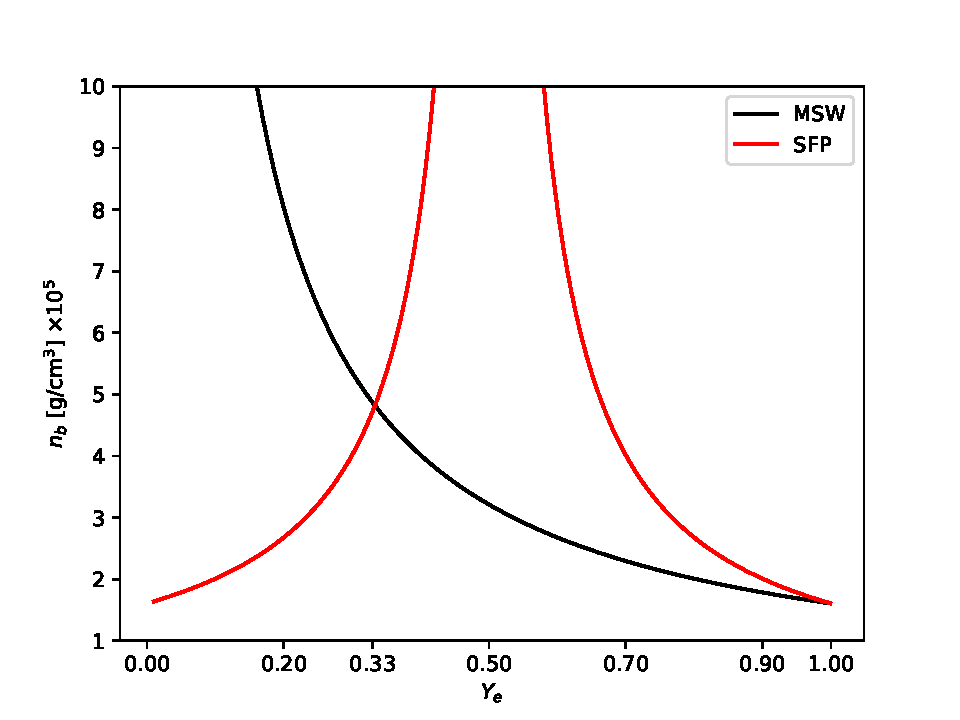
\includegraphics[width=0.8\textwidth]{figures/resonance_nb_Ye.pdf}
	\caption[MSW ve SFP rezonansları]{MSW ve SFP rezonansları. Eğer madde ortamında $ Y_e = 0.33 $, $n_{b}(r) \simeq 5 \times 10^{4} $ g/cm$^{3}$ veya $ Y_e \simeq 1 $, $n_{b}(r) \simeq 2	\times 10^{4} $ g/cm$^{3}$ değerleri mevcut ise MSW ve SFP meydana geldiği uzaklıklar kesişir. Bu şekil $ 1 $ MeV enerjiye ve atmosferik karışım açılarına sahip nötrinolar için hesaplanmıştır. }
	\label{fig:resonance_nb_Ye}
\end{figure}
\begin{figure}[hbt!]
	\centering
	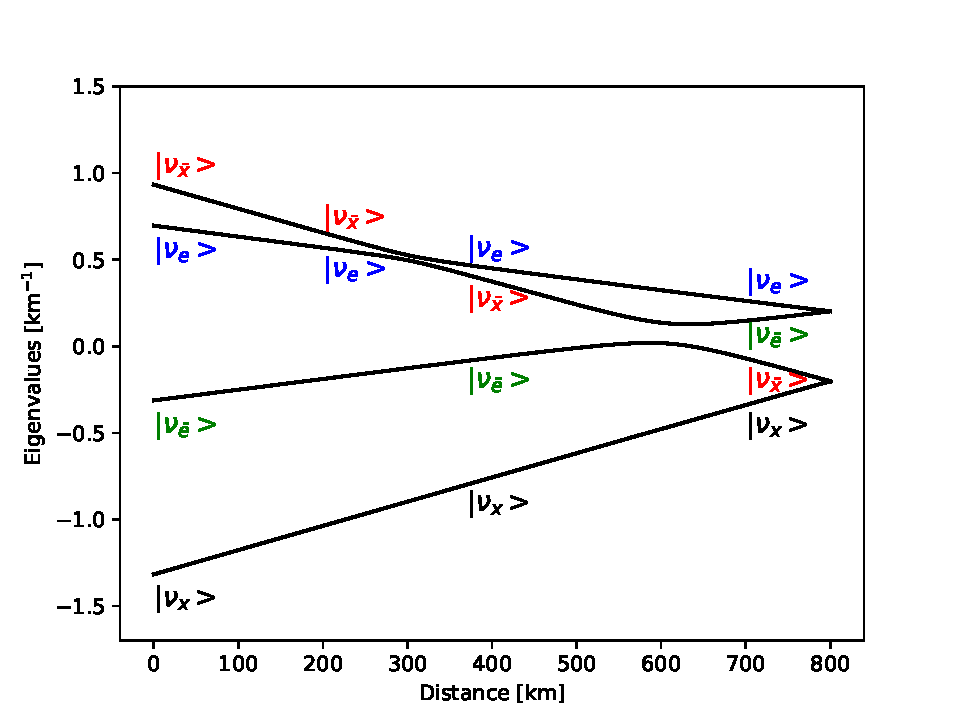
\includegraphics[width=\textwidth]{figures/constant_B_linear_V_flavorContent_16_MeV.pdf}
	\caption[MSW ve SFP Rezonansından geçen nötrinoların çeşni içerikleri]{MSW ve SFP Rezonansından geçen nötrinoların çeşni içerikleri. Bu grafik $ 16 $ MeV için çizilmiştir. Madde profili doğrusal olup manyetik alan ise sabittir.}
	\label{fig:simpleCaseSemiAdiabFlavContent}
  \end{figure}
\newpage
\chapter{ANALİTİK ÖNGÖRÜLER VE SİMÜLASYONLAR}\label{ch:simulasyonlar}
\paragraph{}
Bu tezde altı adet ana simülasyon modelinin sonucu incelenmiştir. Simülasyonların isimlendirilmesi, dikkate alınan etkileşimler ve potansiyellerin konum bağımlılıkları \ref{tab:simulasyonlar} numaralı tabloda yer almaktadır. Simülasyon modelleri, oyuncak model ve gerçekçi model olarak ikiye ayrılmıştır. Oyuncak modeller etkileşim potansiyellerinin analitik formülleri kullanılarak yapılırken, gerçekçi modellerde ÇÇSN simülasyonundan elde edilen sayısal baryon profili kullanılmıştır. 

Öncelikle, oyuncak modeller başlığı altında madde profilinin analitik ifadesi bilinen bir potansiyel için simülasyonlar yapılacaktır. Eksponansiyel olarak azalan madde profili ve $ (50 \text{ km}/r)^{2} $ ile azalan manyetik alan profili altında analitik öngörüler ile sayısal sonuçlar karşılaştırılacaktır. Sonuçları daha iyi anlayabilmek için önce karışım açısının sıfır olduğu, yani boşluk salınımlarının olmadığı durumda, hem analitik hem de sayısal elektron nötrino yaşama olasılıkları elde edilecektir. Ardından küçük bir çeşni karışım açısı altında sonuçların değişimine bakılacaktır. Tüm bunlar \ref{sec:OyuncakModel} numaralı bölümde incelenecektir.

Oyuncak modeller incelendikten sonra \ref{sec:gercekciModeller} numaralı bölümde ÇÇSN'nin gerçekçi madde profili kullanılarak çeşni evrimi incelenecektir. Gerçekçi modeller için \cite{1987ESOC...26..325N} numaralı kaynaktan ön süpernova (pre-supernova) modeli alınıp üzerine şok dalgası eklenmiştir. Şok dalgası ise \cite{Athar:1995cx} numaralı kaynaktaki parametrizasyon yardımı ile madde profiline eklenmiştir.

Gerçekçi modeller için de dört farklı simülasyon yapılmıştır. Simülasyonlarda nötrino öz-kırılımı ve nötrino manyetik alan etkileşiminin kollektif çeşni salınımlarına olan etkisi incelenmiştir. Simülasyonların adlandırılması \ref{tab:simulasyonlar} numaralı tabloda verilmiştir.

\begin{table}[hbt!]
    \centering
    \begin{tabular}{|c|c|c|}
        \hline
         & \textbf{Etkileşimler} & \textbf{Potansiyeller} \\ 
        \hline
        \small{theta0expNbB}   & $M,EM$  & \footnotesize{$n_{b}(r)=10^{6} e^{-r/200 \text{ km}} $ [g/cm$^{3}$], $B\approx 10^{15} \qty(\frac{50 \text{ km}}{r})^{2}$  [Gauss]}\\
        \hline
        \small{theta014expNbB} & $\nu,M,EM$  & \footnotesize{$n_{b}(r)=10^{6} e^{-r/200 \text{ km}} $ [g/cm$^{3}$], $B\approx 10^{15} \qty(\frac{50 \text{ km}}{r})^{2}$  [Gauss]}\\
        \hline
        \small{t5sNoCollnuNoB}  & $\nu,M$ & \cite{1987ESOC...26..325N, Athar:1995cx} kaynaklarından $ t=5 $s için $n_{b}(r)$\\
        \hline
        \small{t5sNoCollnuB}   & $\nu,M,EM$  &\tiny{\cite{1987ESOC...26..325N, Athar:1995cx} kaynaklarından $ t=5 $s için $n_{b}(r)$ ve $B= 10^{15} \qty(\frac{50 \text{ km}}{r})^{2}$ [Gauss]}\\
        \hline
        \small{t5sCollnuNoB}   & $\nu,M,\nu\nu$ &\cite{1987ESOC...26..325N, Athar:1995cx} kaynaklarından $ t=5 $s için $n_{b}(r)$\\
        \hline
        \small{t5sCollnuB}     & $\nu,M,EM, \nu\nu$ &\tiny{\cite{1987ESOC...26..325N, Athar:1995cx} kaynaklarından $ t=5 $s için $n_{b}(r)$ ve $B= 10^{15} \qty(\frac{50 \text{ km}}{r})^{2}$ [Gauss]}\\
        \hline
    \end{tabular}
    \caption[Simülasyon Adlandırılması, Etkileşimler Ve Potansiyeller.]{\label{tab:simulasyonlar}Simülasyon adlandırılması, dikkate alınan etkileşimler ve potansiyellere ait profiller. theta014expNbB adlı modelde, baryon profilinin başlangıçtaki değeri olan $ 10^{6} $ g/cm$^{3}$ değeri ÇÇSN $t=5$ s için olan profilin fit değeridir. Bu modelin altında, başlangıç baryon yoğunluğu farklı olan alt simülasyonlar da yapılmıştır. Ayrıca, theta014expNbB modeli incelenirken normal hiyerarşi ve elektron antinötrino kutu spektrumuna sahip simülasyonlar da yapılmıştır. Manyetik alan profilleri \cite{deGouvea:2012hg,deGouvea:2013zp,Kharlanov:2020cti} numaralı referanslarla uyumludur.}
\end{table}

\section{ANALİTİK ÖNGÖRÜLER}\label{sec:evrim}
\paragraph{}
Bu bölümde, yapılacak olan simülasyonların hareket denklemlerini, özbazdaki ortalama çözümleri ve geçiş olasılıklarını inceleyeceğiz.  Yoğunluk operatörünün başlangıçtaki ifadesi aşağıdaki gibi yazılır.
\begin{align}
    \nonumber \hat{\rho}(R) =& \sum_{i,j} \mel{E_{i}(R)}{\hat{\rho}}{E_{j}(R)} \dyad{\Psi_{i}(R)}{\Psi_{j}(R)} \text{ ,}\\
    = & \sum_{i,j} \rho_{ij}(R) \dyad{\Psi_{i}(R)}{\Psi_{j}(R)} \text{ .}
\end{align}
Burada $ \ket{E_{i}(R)} $ sistemin başlangıçtaki özvektörü, $ \Psi_{i}(R) $ ise nötrinoların başlangıçtaki durum ketidir. Bu çalışmada, aksi belirtilmedikçe başlangıç nötrino durum keti, ya sadece elektron nötrino olarak ya da sadece elektron antinötrinosu olarak tanımlanacaktır. Yoğunluk operatörünü herhangi bir uzaklıktaki ifadesini yazmak için durum ketini evrimleştirmek gerekmektedir.
\begin{equation}\label{eqn:psiAexp}
    \ket{\Psi_{i}(r)} = \sum_{a} A^{\dagger}_{ia}(r) \exp(-i\int^{r}_{R} E_{a}(x) \dd{x}) \ket{E_{a}(r)} \text{ .}
\end{equation}
$ A $ matrisi, evrimin adyabatikliğini belirleyen, \eqref{eqn:LZamplitude} numaralı denklemde tanımlanan, özvektörler arasındaki geçişi veren LZ geçiş genlik matrisidir. 

Nötrinolar evrimlerini bir özbazda başlayıp bitirebilir. Bu durum, başlangıçtaki özbazda yazılan yoğunluk matrisinin, köşegen elemanlarının değişmeden aynı kalması anlamına gelir. Bir önceki bölümde bu çeşit evrime adyabatik evrim adı verilmişti. Bir diğer taraftan, nötrinolar belli bir uzaklığa geldiğinde, o uzaklıktaki özvektörler, başlangıçtaki özvektörlerin bir süper pozisyonu olabilir. Bu durum da adyabatiklikten sapma olarak belirtebiliriz. Son olarak özvektörler yer değiştirebilir. Bu da evrimin diabatik olduğu anlamına gelir.

\eqref{eqn:psiAexp} numaralı denklemde $ E_{a}(r) $, sistemin $ r $ uzaklığındaki özdeğerleridir. Tüm eksponansiyel terim evrimin salınım fazını oluşturur. Yoğunluk operatörü, $ r $ uzaklığına geldiğinde 
\begin{align}
    \nonumber \hat{\rho}(r) =& \sum_{a,b}\sum_{i,j} \qty(A_{ai}(r) \rho_{ij}(R) A^{\dagger}_{jb}(r))\exp(-i\int^{r}_{R} \qty(E_{a}(x)- E_{b}(x)) \dd{x})\\ 
    \nonumber &\times \dyad{E_{i}(r)}{E_{j}(r)} \text{ ,} \\
    =& \sum_{a,b}\sum_{i,j}\qty(A_{ai}(r) \rho_{ij}(R) A^{\dagger}_{jb}(r)) C_{ij}(E)
    \dyad{E_{i}(r)}{E_{j}(r)} \text{ ,}
\end{align}
şeklinde olacaktır. Evrime gelen salınım fazı, $ C_{ij}(E) $, sadece enerji özdeğerlerine bağlıdır. Bu faz çeşni bazında yazılan yaşama olasılığında ortalama bir değer üzerinde salınıma sebep olur. Yoğunluk operatörünü ortalama kısmı, $ \hat{\bar{\rho}}(r) $, ve salınan kısmı, $ \hat{\rho}_{sal}(r) $, olarak iki şekilde yazabiliriz.
\begin{align}\label{eqn:rhoBar_rhoSal}
    \nonumber \hat{\rho}(r) = & \hat{\bar{\rho}}(r) + \hat{\rho}_{sal}(r) \text{ ,}\\
    \nonumber               = &   \sum_{a}\sum_{i,j}\qty(A_{ai}(r) \rho_{ij}(R) A^{\dagger}_{ja}(r)) \dyad{E_{i}(r)}{E_{j}(r)} \\
                              & + \sum_{\substack{a,b\\ a \ne b}}\sum_{i,j}\qty(A_{ai}(r) \rho_{ij}(R) A^{\dagger}_{jb}(r)) C_{ij}(E) \dyad{E_{i}(r)}{E_{j}(r)} \text{ .}
\end{align}

Yoğunluk operatörün ortalama kısmı evrim hakkında genel bir fikir vermemizi sağlar. Özellikle çok uzaklardan gelen kaynaklarda, na-eş evreli (decoherance) kaynaklı çeşni salınım kısmı sıfıra inecektir \cite{GIUNTI199287, Hansen:2016klk}. Çeşni evrimi sırasında nötrinolar, bir özbazdan başka bir özbaza atlarsa salınımların etkisi ortaya çıkacaktır. 

Özdurumların yerine tedirgeme teorisinden elde ettiğimiz \eqref{eqn:EMbasisKets} numaralı ifadeleri koyabiliriz. Bu durumda yoğunluk operatörünün çeşni tabanındaki ifadesini yaklaşık olarak elde edebiliriz. Ortalama yoğunluk operatörünün $ ee $ tabanına izdüşümü, adyabatik bir evrim için aşağıdaki gibi verilir.
\begin{align}
    \nonumber\rho_{ee}(r)  =& \sum_{i} \rho_{ii}(R) \braket{\nu_{e}}{\nu_{i}^{EM}(r)} \braket{\nu_{i}^{EM}(r)}{\nu_{e}} \\
    \nonumber=& \frac{\rho_{11}(R) c^{2}_{\theta_{M}}}{N^{2}_{1}}+ \frac{\rho_{22}(R) s^{2}_{\theta_{M}}}{N^{2}_{2}}+ \frac{\rho_{33}(R) \mu^{2} B^{2}}{N^{2}_{3}} \qty(\frac{s_{\gamma} c_{\theta_{M}}}{\delta \omega_{31}}+\frac{c_{\gamma} s_{\theta_{M}}}{\delta \omega_{32}})^{2}\\
    &+ \frac{\rho_{44}(R) \mu^{2} B^{2}}{N^{2}_{4}} \qty(\frac{c_{\gamma} c_{\theta_{M}}}{\delta \omega_{41}}+\frac{s_{\gamma} s_{\theta_{M}}}{\delta \omega_{42}})^{2}
\end{align}
Burada LZ geçiş genlik matrisi $ A $, birim matris olarak tanımlanarak adyabatik evrim varsayılmıştır.

Nötrinoların içerisinden geçtiği ortam çok ani değiştiğinde veya bir süreksizlik meydana geldiğinde evrim bir özbazdan başka bir özbaza geçecektir. Bu yeni özbaz evrimin geri kalanından sorumlu olacak ve çeşni evrimini belirleyecektir. Bu örnek, iki farklı başlangıç koşulu ve iki farklı simülasyonun birleştirilmesi olarak düşünülebilir. Bu süreksizliğin olduğu noktanın öncesindeki ve sonrasındaki yoğunluk operatörlerinin birleştirilmesi gerekmektedir.

Yukarıda bahsedilen süreksizlik, elektron kesrinin ani değişmesinden kaynaklanabilir. ÇÇSN oluşmadan önce ve oluştuğu ilk saniyelerde elektron kesrinin belli bir $ r_{d} $ değerinde çok hızlı değişmesi gerektiği düşünülmektedir \cite{Athar:1995cx}. Bu değerden kaynaklı çeşni evriminde bir süreksizlik meydana gelecektir. 

Ani değişimin yaşandığı $ r_{d} $ uzaklığının öncesindeki özvektörlere $ \ket{E_{i}} $, sonrasındaki özvektörlere de $ \ket{E'_{i}} $ adını verelim. Basitlik olması açısından, nötrinoların arka planda meydana gelen ani değişime kadar ve ani değişimden sonraki evrimi adyabatik olsun. Yani LZ geçiş matrisi, $ A(r) $, süreksizlikten önce ve sonra birim matris olsun. Bu durumda yoğunluk operatörü $ r_{d} $ uzaklığına kadar aşağıdaki gibi yazılır.
\begin{align}
    \nonumber \hat{\rho}(r) = \sum_{i,j,k,l} \qty[\rho_{ij}(R) C_{ij}(E) C'_{kl}(E)]~ \dyad{E'_{k}(r)}{E'_{l}(r)} \\
    \times \dyad{E'_{k}(r)}{E_{i}(r_{d})} \dyad{E_{j}(r_{d})}{E'_{l}(r)} \text{ .}
\end{align}
Burada $ C'_{kl} = \exp(-i\int^{r}_{r_{d}} \qty(E'_{k}(x)- E'_{l}(x)) \dd{x}) $ şeklindedir. Ani değişim yaklaşıklığında, Hamiltonyen aniden değiştiğinde, yoğunluk operatörünün evrimi aniden değişmiyor veya değişmek için yeterli zamanı olmuyor \cite{messiah2014quantum}. Süreksizlikten sonra $ C_{ij}(E) $ terimi salınım yapmayı bırakır. Süreksizlik noktasına kadar gelen salınım fazına \emph{donmuş faz} (frozen phase) adı verilecektir. Çeşni bazına geçtiğimizde donmuş fazın bilgisi, $ r_{d} $ uzaklığından sonra da kalır. Donmuş faz nedeniyle salınan yaşama olasılığı, $ r_{d} $ değerine geldiğinde bambaşka bir faz ile salınmaya başlar. İşte bulduğumuz bu donmuş fazın varlığı ve $ r_{d} $ noktasındaki değeri, süreksizlikten sonra da etkisini göstermektedir. Öte yandan $ C'_{kl}(E) $ salınım fazı, süreksizlik noktasından sonra kazandığı fazdır ve bir ortalamanın etrafında salınır. Eğer ikinci bir süreksizlik yoksa $ C'_{kl}(E) $ fazı sadece salınım terimlerini verecektir. 

Süpernova ortamında elektron kesrinin süreksizliği gibi baryon kütlesinin süreksizliği de oluşmaktadır. Bu süreksizliği yaratacak olan en büyük değişim şok dalgasının ön yüzü olacaktır. Şok dalgasının, süpernova merkezinden dışarı doğru bakan bölümü yani ön yüzündeki değişim nötrinoların çeşni evrimini etkiler ancak yukarıda bahsedildiği gibi bir değişme sebep olmaz. Gerçekçi modeller bölümünde bu konu daha ayrıntılı incelenecektir.

Donmuş fazların etkisine ve çeşni evrimine daha ayrıntılı bakabilmek için yoğunluk operatörünü çeşni tabanında yazmak gerekmektedir. ÇÇSN'nin iç kısımlarına baktığımızda manyetik moment etkisiyle $ e-\bar{x} $ veya $ x-\bar{e} $ geçişleri olabilir. Sadece $ e-\bar{x} $ geçişleri dikkate alındığında enerji özdurumlarından $ \ket{E_{1,2}} $ ve $ \ket{E'_{1,2}} $ baskındır. O halde iki duruma indirgenmiş yoğunluk matrisi aşağıdaki gibi yazılır.
\begin{equation}
    \hat{\overline{\rho}}(r) = \sum^{2}_{i,j,k} C_{ij}(E) \rho_{ij}(R) ~\dyad{E'_{k}(r)}{E_{i}(r_{d})} \dyad{E_{j}(r_{d})}{E'_{k}(r)} \dyad{E'_{k}(r)}{E'_{k}(r)} \text{ .}
\end{equation}
Burada $ k=l $ şeklide alındığı için $C'_{kl} $ terimi atılmıştır. Madde arka planın çok büyük olduğu bir ortamda özvektörler neredeyse çeşni tabanındadır. Bunu, nötrinoların salınım yapamadan madde ile etkileşerek sürekli çeşni tabanında olmaya zorlanması gibi görülebilir. Bu çalışmada genelliği bozmamak için özvektörleri iki farklı çeşninin süperpozisyonu olarak alacağız. Başlangıçta, manyetik alan güçlü olduğundan dolayı özdurumlar çeşni tabanından bir miktar sapabilir. Bundan dolayı şunu yazabiliriz.
\begin{align}
    \ket{E_{1}(r_{d})} =& \cos{\theta_{EM}(R)} \ket{\nu_{\bar{x}}} + \sin{\theta_{EM}(R)} \ket{\nu_{e}} \text{ ,} \\
    \ket{E_{2}(r_{d})} =&-\sin{\theta_{EM}(R)} \ket{\nu_{\bar{x}}} + \cos{\theta_{EM}(R)} \ket{\nu_{e}} \text{ ,} \\
    \ket{E'_{1}(r)} =& \cos{\theta_{EM}(r)} \ket{\nu_{\bar{x}}} + \sin{\theta_{EM}(r)} \ket{\nu_{e}}    \text{ ,} \\
    \ket{E'_{2}(r)} =&-\sin{\theta_{EM}(r)} \ket{\nu_{\bar{x}}} + \cos{\theta_{EM}(r)} \ket{\nu_{e}} \text{ .}
\end{align}
Cebirsel işlemler yapıldığında öz tabanındaki yoğunluk operatörü, çeşni tabanında yazılabilir.
\begin{align}
    \nonumber \hat{\overline{\rho}}(r) = &\qty(\alpha_{11}\cos^{2}\theta_{EM}(r) + \alpha_{22}\sin^{2}\theta_{EM}(r) ) \dyad{\nu_{\bar{x}}}{\nu_{\bar{x}}} \\
    \nonumber &+ \qty(\alpha_{11}\sin^{2}\theta_{EM}(r) + \alpha_{22}\cos^{2}\theta_{EM}(r) ) \dyad{\nu_{e}}{\nu_{e}} \\
    &+ \qty(\alpha_{11}\sin{2\theta_{EM}(r)} - \alpha_{22}\sin{2\theta_{EM}(r)} ) \qty(\dyad{\nu_{e}}{\nu_{\bar{x}}} + \dyad{\nu_{\bar{x}}}{\nu_{e}})  \text{ .}
\end{align}
Burada $ \alpha_{11} $ ve $ \alpha_{22} $ aşağıdaki gibi tanımlanır.
\begin{align}
    \nonumber \alpha_{11} =& \rho_{11}(R)\cos^{2}\qty(\theta_{EM}(R) - \theta_{EM}(r)) \\
    \nonumber             &+ \rho_{22}(R)\sin^{2}\qty(\theta_{EM}(R) - \theta_{EM}(r)) \\
                &+ \rho_{12}\frac{C_{12}+C_{21}}{2}\sin\qty(2\qty(\theta_{EM}(R) - \theta_{EM}(r))) \text{ ,}\\
    \nonumber \alpha_{22} =&-\rho_{11}(R)\sin^{2}\qty(\theta_{EM}(R) - \theta_{EM}(r)) \\
    \nonumber &+ \rho_{22}(R)\cos^{2}\qty(\theta_{EM}(R) - \theta_{EM}(r)) \\
                &- \rho_{12}\frac{C_{12}+C_{21}}{2}\sin\qty(2\qty(\theta_{EM}(R) - \theta_{EM}(r))) \text{ .}
\end{align}

Elde edilen sonuçlar, $ 2\times2 $'ye indirgenebilen $ 1-4 $ Hamiltonyen'i için ve adyabatik evrim varsayımı altında türetilmiştir. Dört çeşni için yaklaşık çözümler tedirgeme kuramından elde edilen özvektörler kullanılarak yazılır.

Geçiş matrisini birim matristen farklı aldığımızda, nötrino yaşama olasılıklarına LZ geçiş olasılıkları dahil olacaktır. Bu sefer LZ geçiş olasılıklarını sisteme dahil ederken salınım terimi $ C_{ij} $ terimi ortalamaya girmez. İki çeşniye indirgenmiş ortalama yoğunluk operatörü \eqref{eqn:rhoBar_rhoSal} numaralı denklem kullanılarak aşağıdaki gibi yazılır.
\begin{align}
    \nonumber \hat{\bar{\rho}}(r) =& \big[(1-P_{LZ})\rho_{11}(R)+P_{LZ}\rho_{22}(R) \\
    \nonumber & ~~ -\qty(e^{i\varphi}\rho_{12}+e^{-i\varphi}\rho_{21}(R)) \sqrt{P_{LZ}(1-P_{LZ})}\big] \dyad{E_{1}(r)}{E_{1}(r)} \\
    \nonumber & \big[P_{LZ}\rho_{11}(R)+(1-P_{LZ})\rho_{22}(R) \\
    & ~~ +\qty(e^{i\varphi}\rho_{12}+e^{-i\varphi}\rho_{21}(R)) \sqrt{P_{LZ}(1-P_{LZ})}\big] \dyad{E_{2}(r)}{E_{2}(r)} \text{ .}
\end{align}
Burada $ \varphi $ terimi Stokes fazdır ve özvektörlerin birbirine geçmesinden gelir. Matematiksel olarak düşünürsek, geçiş genliği $ A $ matrisinin sanal tanımlı olmasından kaynaklıdır. Stokes fazı, aşağıdaki koşul sağlandığında evrimde kendini göstermeyecektir.
\begin{equation}\label{eqn:phaseDisapearCond}
    \frac{(1-P_{LZ}) \rho_{11}(R) + P_{LZ} \rho_{22}(R)}{\sqrt{P_{LZ}(1-P_{LZ})}\rho_{12}(R)} \gg 1 \text{ .}
\end{equation}
LZ geçiş olasılık formülü, \ref{ch:Rezonanslar} bölümünde elde edilirken üç adet yaklaşımdan bahsedilmişti. \eqref{eqn:phaseDisapearCond} numaralı denklemdeki koşul, ikinci yaklaşıklığın sağlanmadığı durumlarda geçerli olur. Yani başlangıçta durum keti Hamiltonyen'in özdurumunda değilse yaşama olasılığına Stokes fazları gelecektir. Başlangıç koşullarında yapılan küçük değişiklikler ise çeşni evriminin son halinde farklılıklara sebep olacaktır. \ref{sec:OyuncakModel} numaralı bölümde, 9 farklı başlangıç koşulu alınarak fazlardan kaynaklanan değişim gösterilecektir.

SFP rezonansının adyabatik olmaması gibi MSW rezonansı da adyabatik olmayabilir. Bu durumda $ A $ matrisi iki farklı rezonans matrisinin çarpımı olacaktır. Bu tezde, aksi belirtilmedikçe, ters hiyerarşi ve $ Y_{e}<0.5 $ değeri göz önüne alındığından dolayı $ A $ matrisini oluşturan LZ rezonans geçiş matris çarpım sırası aşağıdaki gibi olur.
\begin{align}
    \nonumber A =& A_{SFP} \times A_{MSW} \text{ ,}\\
      =& \mqty(\sqrt{1-P_{SFP}} & -e^{-i\alpha}\sqrt{P_{SFP}} & 0 & 0 \\
      e^{i\alpha}\sqrt{P_{SFP}} & \sqrt{1-P_{SFP}} & 0 & 0 \\ 0 & 0 & 1 & 0 \\ 0 & 0 & 0 & 1) \times
      \mqty(1 & 0 & 0 & 0 \\ 0 & \sqrt{1-P_{MSW}} & -e^{-i\beta}\sqrt{P_{MSW}} & 0 \\ 0 & e^{i\beta}\sqrt{P_{MSW}} & \sqrt{1-P_{MSW}} & 0 \\ 0 & 0 & 0 & 1) \text{ .}
\end{align}
Burada $ A_{SFP} $ matrisi $ P_{SFP} $ geçiş olasılıkları ve $ \alpha $ fazına sahiptir. $ A_{MSW} $ matrisi ise $ P_{MSW} $ ve $ \beta $ fazına sahiptir. Bu denklem ancak ve ancak SFP ve MSW rezonansları birbirlerinden "yeterince" ayrı olduklarında doğrudur. Rezonansların birbirlerinden ne kadar ayrıldığı  \ref{sec:OyuncakModel} numaralı bölümde belirlenecektir. 

Geçiş genliğini \eqref{eqn:rhoBar_rhoSal} numaralı denklemde yerine koyup tüm elemanları açık açık yazabiliriz. Bu işlemi yaparken salınım fazı $ C_{ij}(E) $ terimini ise katacağız. Yani geçiş matrislerini sırayla ekleyeceğiz.
\begin{align}
    \rho_{ij}(R)C_{ij}(E) \rightarrow& A^{\dagger}_{SFP}\rho_{ij}(R)C_{ij}(E)~A_{SFP}\\
    \rightarrow& A^{\dagger}_{SFP} ~ \rho_{ij}(R)C_{ij}(E)~A_{SFP} C'_{ij}(E)\\
    \rightarrow& A^{\dagger}_{MSW}A^{\dagger}_{SFP}~\rho_{ij}(R)C_{ij}(E)~A_{SFP} C'_{ij}(E)~A_{MSW} \text{ .}
\end{align}
Denklemleri bu şekilde kurduğumuzda donmuş fazlar dahil neredeyse tüm fazları yoğunluk operatörüne koyuyoruz. Tek dahil etmediğimiz faz, en uzakta meydana gelen MSW rezonansından sonra ortalamaya gelen salınım fazıdır.

Denklemlerin açık ifadesini yazarken ortalama yoğunluk operatörünün öz tabandaki halini üç terime ayıracağız. Bunlardan birincisi ortalama değer, $ \hat{\overline{\rho}}_{\text{ort}} $ olacaktır. İkincisi ise ortalama değerden sapma yani fazlardan kaynaklanan fark olacaktır. Bu terimdeki fazlar başlangıç koşullarına çok hassas şekilde bağlı olduğu için Dünya'da gözlemlenecek her bir nötrino için farklı olacaktır. Bu nedenle kendini bir çeşit ölçüm hatası (error bar) gibi gösterecektir. Biz buna analitik öngörünün \emph{hatası} olarak adlandıracağız ve $ \hat{\overline{\rho}}_{\text{hata}} $ olarak göstereceğiz. Son olarak ortalama etrafındaki salınımları veren köşegen olmayan terimler olacaktır. Bu terime de $ \hat{\overline{\rho}}_{\text{naKos}} $ adı verilecektir. Ortalama yoğunluk operatörü,
\begin{equation} \label{eqn:ortYogun1}
    \hat{\overline{\rho}}(r) = \hat{\overline{\rho}}_{\text{ort}}(r) + \hat{\overline{\rho}}_{\text{hata}}(r) + \hat{\overline{\rho}}_{\text{naKos}}(r) \text{ ,}
\end{equation}
şeklinde yazabiliriz. Bu terimlerden ortalama terim aşağıdaki gibi yazılır.
\begin{align}\label{eqn:rhoBar_ort}
    \nonumber\hat{\overline{\rho}}_{\text{ort}}=& \bigg[(1-P_{SFP}) \rho_{11}(R)+ P_{SFP} \rho_{22}(R)\bigg] \dyad{E_{1}(r)}{E_{1}(r)}\\
    \nonumber&+ \bigg[\qty(1-P_{MSW})\qty(P_{SFP}\rho_{11}(R) +(1-P_{SFP})\rho_{22}(R))\\
    \nonumber&~~~+ P_{MSW} \rho_{33}(R)\bigg] \dyad{E_{2}(r)}{E_{2}(r)}\\
    \nonumber&+ \bigg[P_{MSW}\qty(P_{SFP}\rho_{11}(R)+ (1-P_{SFP})\rho_{22}(R))\\
    \nonumber&~~~+(1-P_{MSW})\rho_{33}(R)\bigg] \dyad{E_{3}(r)}{E_{3}(r)}\\
    &+ \rho_{44}(R) \dyad{E_{4}(r)}{E_{4}(r)} \text{ .}
\end{align}
Ortalama yoğunluk operatöründen de görüleceği üzere dördüncü özdurum ki, ters hiyerarşi ve $ Y_{e}<0.5 $ değeri göz önüne alındığında içerisinde en fazla $ x $ çeşnisinden bulunur,  diğerlerinden ayrışacaktır. İlk önce SFP rezonansı meydana geldiği için birinci özdurum ile ikinci özdurum karışır. Ardından gerçekleşecek olan MSW rezonansından birinci özdurum etkilenmez. İkinci ve üçüncü özdurum SFP rezonansından sonra MSW rezonansından da geçtiği için hem $ P_{MSW} $ hem de $ P_{SFP} $ terimlerine sahiptir. 

Stokes ve salınım fazlarından kaynaklanan terimler ise yukarıdaki verilen formül etrafında salınımlara neden olacaktır. Dikkat edilmesi gereken konu, köşegen terimlere gelen katkılar fazlardan kaynaklıdır ve salınımlarla alakası yoktur. Yani $ \hat{\overline{\rho}}_{\text{ort}}+ \hat{\overline{\rho}}_{\text{hata}} $ terimlerinde $ i \ne j$ için $ \dyad{E_{i}(r)}{E_{j}(r)} $ terimleri bulunmamaktadır. $ \hat{\overline{\rho}}_{\text{hata}}(r) $ operatörü,
\begin{align}\label{eqn:rhoBar_hata}
    \nonumber\hat{\overline{\rho}}_{\text{hata}}(r)=&\pm 2\bigg[\sqrt{(1-P_{SFP}) P_{SFP}}\rho_{12}(R)]\\
    \nonumber&~~\times[(1-P_{MSW})\dyad{E_{2}(r)}{E_{2}(r)} -\dyad{E_{1}(r)}{E_{1}(r)}\bigg]\\
    \nonumber&\pm 2\bigg[\sqrt{(1-P_{MSW})P_{MSW}}\qty(\sqrt{P_{SFP}}\rho_{13}(R)+\sqrt{1-P_{SFP}}\rho_{23}(R))\bigg]\\ \nonumber& ~~\qty[\dyad{E_{3}(r)}{E_{3}(r)} - \dyad{E_{2}(r)}{E_{2}(r)}]\\
    &\pm 2 \bigg[P_{MSW}\sqrt{(1-P_{SFP}) P_{SFP}} \rho_{12}(R)\bigg]\dyad{E_{3}(r)}{E_{3}(r)} \text{ ,}
\end{align}
şeklinde yazılır. Burada fazlardan kaynaklanan eksponansiyel terimlerin maksimum ve minimum değerleri göz önüne alınmıştır. Bundan dolayı her bir terimin başına $ \pm $ terimleri gelmiştir. Ayrıca yoğunluk operatörünün $ \rho_{ij}(R) = \rho_{ji}(R)$ özelliğini kullanıp, eksponansiyel terimler yerine kosinüs koyduğumuzda $ 2 $ katsayısı gelir.

Son olarak köşegen olmayan terimler ise aşağıdaki gibi yazılır.
{\footnotesize
\begin{align}
    \nonumber\hat{\overline{\rho}}_{\text{naKos}}(r) =&\pm 2 \bigg[\sqrt{1-P_{MSW}} [\sqrt{\qty(1-P_{SFP}) P_{SFP}}\rho_{11}(R)+ \qty(1-P_{SFP})\rho_{12}(R)\\
    \nonumber &~~-\qty(P_{SFP}\rho_{21}(R)+\sqrt{\qty(1-P_{SFP}) P_{SFP}} \rho_{22}(R))\big]\\
    \nonumber &~~-\sqrt{P_{MSW}} \qty(\sqrt{1-P_{SFP}}\rho_{13}(R)-\sqrt{P_{SFP}} \rho_{23}(R))\bigg]\dyad{E_{1}(r)}{E_{2}(r)}\\
    \nonumber&\pm 2 \bigg[\sqrt{P_{MSW}} \bigg(\sqrt{\qty(1-P_{SFP})P_{SFP}} \rho _{11}(R) +\qty(1-P_{SFP})\rho_{12}(R)\\
    \nonumber &~~-\qty(P_{SFP}\rho_{21}(R)+\sqrt{\qty(1-P_{SFP})P_{SFP}}\rho _{22}(R))\bigg)\\
    \nonumber &~~ +\sqrt{1-P_{MSW}} \qty(\sqrt{1-P_{SFP}}\rho_{13}(R)-\sqrt{P_{SFP}}\rho _{23}(R))\bigg] \dyad{E_{1}(r)}{E_{3}(r)}\\
    \nonumber&\pm 2\bigg[\sqrt{1-P_{SFP}}\rho_{14}(R)-\sqrt{P_{SFP}}\rho _{24}(R)\bigg] \dyad{E_{1}(r)}{E_{4}(r)}\\
    \nonumber&\pm 2\bigg[\sqrt{\qty(1-P_{MSW}) P_{MSW}} \bigg(\sqrt{\qty(1-P_{SFP})P_{SFP}} \rho_{12}(R)\\
    \nonumber&~~+\sqrt{\qty(1-P_{SFP}) P_{SFP}} \rho_{21}(R)+P_{SFP}\qty(\rho_{11}(R)-\rho_{22}(R))+\rho_{22}(R)\bigg)\\
    \nonumber&~~+\qty(1-P_{MSW}) \qty(\sqrt{P_{SFP}} \rho _{13}(R)+ \sqrt{1-P_{SFP}} \rho_{23}(R))\\
    \nonumber&~~-P_{MSW} \qty(\sqrt{P_{SFP}} \rho _{31}(R)+ \sqrt{1-P_{SFP}}\rho _{32}(R))\\
    \nonumber&~~-\sqrt{\qty(1-P_{MSW})P_{MSW}} \rho _{33}(R)\bigg] \dyad{E_{2}(r)}{E_{3}(r)}\\
    \nonumber&\pm 2[\sqrt{1-P_{MSW}} \qty(\sqrt{P_{SFP}}\rho_{14}(R)+\sqrt{1-P_{SFP}}\rho_{24}(R))\\
    \nonumber&~~-\sqrt{P_{MSW}}\rho_{34}(R)]\dyad{E_{2}(r)}{E_{4}(r)}\\
    \nonumber&\pm 2[\sqrt{P_{MSW}} \qty(\sqrt{P_{SFP}}\rho_{14}(R)+\sqrt{1-P_{SFP}}\rho_{24}(R))\\
    &~~+\sqrt{1-P_{MSW}}\rho_{34}(R)]\dyad{E_{3}(r)}{E_{4}(r)} \text{ .}
\end{align}}

Köşegen olmayan terimlerin en büyük ve en küçük terimleri çeşni bazındaki salınımların etrafını sarmalayan zarfı verecektir. Bu tezdeki sayısal-analitik hesap karşılaştırılmalarında bu terim dikkate alınmayacaktır.

Son olarak, \eqref{eqn:ortYogun1} numaralı denklem ile verilen ortalama yoğunluk operatöründeki "ortalama" kelimesi ile \eqref{eqn:rhoBar_ort} numaralı denklemdeki "ortalama" kelimesinin farklı durumlarda kullanıldığını belirtmek isteriz. \eqref{eqn:rhoBar_ort} numaralı denklemdeki ortalama, evrimin MSW rezonansı bitene kadar olan uzaklıktaki ortalama yoğunluk matrisini kapsamaktadır. Yoğunluk operatörünün ortalaması ise tüm evrimin ortalaması anlamına gelmektedir. Yani MSW rezonansından sonra meydana gelen salınımların ortalamasıdır.

Geometrik faz kuantum sistemlerin genel özelliğidir ve eğer Hamiltonyen iki veya daha fazla konuma (zamana) bağlı parametresi varsa açığa çıkabilir. Eğer sistem faz uzayında kapalı bir eğri üzerinde hareket ederse dinamik faza geometrik faz eklenir. SFP rezonanslarında geometrik fazlar ilk olarak \cite{Vidal:1990fr, Smirnov:1991ia, Akhmedov:1991vj} numaralı makalelerinde çalışılmıştır. 

\subsection{GEOMETRİ}\label{subsec:geometri}
\paragraph{}
Kinematik bölümünde, \eqref{eqn:NuKim_LiouvilleVonNeumann} numaralı denklemde, Liouville - von Neumann denklemini yazmıştık. Saçılmaları ihmal ettiğimizde, denklemin açıya bağlı şekli aşağıdaki gibi olur \cite{Duan:2006an, Mirizzi:2015fva}.
\begin{align}\label{eqn:NuKim_LiouvilleVonNeumann_multiAng}
	 i \qty(\vec{v} \vdot \vec{\nabla}) \hat{\rho} = \comm{\hat{H}}{\hat{\rho}} \text{.}
\end{align}
Burada $ \vec{v} $, nötrinoların hız vektörüdür. \eqref{eqn:NuKim_LiouvilleVonNeumann} numaralı denklemi \eqref{eqn:NuKim_LiouvilleVonNeumann_multiAng} numaralı denklemin özel halidir. En genel olarak nötrinolar etkileşim potansiyelleri ile farklı hızlarda ve/veya açılarda girebilir.

Süpernova oluşmadan hemen önce merkezdeki küresel simetrik ve kompakt çekirdeğe proto-nötron yıldızı adı verilmektedir. Proto-nötron yıldızının merkezinde nötrinolar, diğer tüm parçacıklar gibi termal dengeye ulaşmıştır \cite{Janka:2006fh}. Yıldız çekirdeğinin öyle bir katmanı vardır ki nötrinolar etkileşim dengesinden çıkar ve dışarıya doğru hareket ederler. Bu noktaya nötrinosfer (neutrinosphere) adı verilmektedir. Bu çalışmada ele alınan nötrinoların başlangıç noktası nötrinosfer katmanıdır. Bu katman, ata yıldızın kütlesine göre değişiklik gösterse, merkezden yaklaşık $20$ - $50$ km ötede bulunur \cite{Janka:2006fh, Dasgupta:2008cd}.

Nötrinosferden çıkan nötrinoların izotropik olarak yayıldığı varsayılmaktadır.. Bunun anlamı, sistemdeki nötrinolar \emph{her yönde} eşit ağırlıkla yayılmaktadır. Yayılan nötrinolar ise ortam ile etkileşirken tek bir açı ile saçılmaz. Bundan dolayı \eqref{eqn:NuKim_LiouvilleVonNeumann_multiAng} numaralı denklemde $ \vec{v} \vdot \vec{\nabla} $ terimi bulunmaktadır. Bu terimden kaynaklanan katkıyı sadece nötrino potansiyeli için, yani nötrino öz-kırılımı için inceleyeceğiz.

Nötrinosferin şematik yapısı \ref{fig:BulbModel} numaralı şekilde gösterilmiştir. \ref{fig:BulbModel} numaralı şekilde verilen nötrinosfer ve nötrinoların ilerleme modeline \emph{ampul modeli} adı verilir ve \cite{Duan:2006an} numaralı kaynakta geliştirilmiştir. Bu bölümde, bahsedilen referanstaki çıkarım yöntemi üzerinden gidilecektir. Not etmek gerekir ki, sadece bu bölümde $ \theta $, nötrino salınım karışım açısı değil saçılma açısıdır.
\begin{figure}[hbt!]
    \centering
    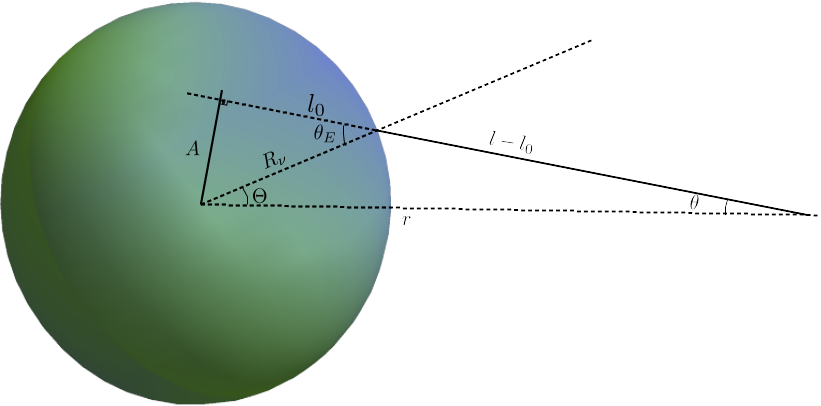
\includegraphics[width=0.7\textwidth]{figures/BulbModel.png}
    \caption[Ampul (Bulb) Modeli.]{Ampul (Bulb) Modeli. Bu şekil \cite{Duan:2006an} numaralı referanstan benzetilerek oluşturulmuştur.}
    \label{fig:BulbModel}
\end{figure}
Ampul modelinin temelde iki adet simetrisi vardır. Birincisi küresel simetri ikincisi ise radyal doğrultuda azimuthal simetridir. Azimuthal simetri, sistemin azimuthal açısından yani $ \varphi $ açısından bağımsız olduğu anlamına gelir. Buradaki $ \theta $ ve $ \varphi $ açıları küresel koordinatlardan gelen açılardır, $ \dd{\vec{r}} = \dd{r} \hat{r} + r\dd{\theta} \hat{\theta} + r\sin\theta\dd{\varphi} \hat{\varphi}  $.  Bu simetrileri, \eqref{eqn:NuKim_LiouvilleVonNeumann_multiAng} numaralı denkleme uygularsak
\begin{equation}
    i v_{r} \dv{r}\hat{\rho} = \comm{\hat{H}}{\hat{\rho}} \text{.}
\end{equation}
denklemi elde edilir. Burada $ v_{r} $, hız vektörünün radyal bileşenidir. Hareket denklemini hızdan bağımsız hale getirip saçılım açısı $ \theta $ ile alakalı hale getirmek için sinüs teoremi kullanılır. 
\begin{equation}
    \frac{\sin \theta}{R_{\nu}} = \frac{\sin \Theta}{l-l_{0}} \text{ .}
\end{equation}
Burada $ l= r\cos \theta $ ve $ l_{0} = R_{\nu} \cos \theta_{E} $ şeklindedir. $ R_{\nu} $ ise nötrinosferin yarıçapıdır ve nötrino evriminin başladığı uzaklıktır. Açıların geometri üzerindeki yerleri, \ref{fig:BulbModel} şeklinde gözükmektedir. $ \sin \theta_{E} $ ve $ \sin \theta $ arasındaki ilişki de aşağıdaki gibi yazılır.
\begin{align}
    \dfrac{\sin \theta}{R_{\nu}} = \dfrac{\sin \theta_{E}}{r} \text{ .}
\end{align}
Tüm bu ilişkiler bir araya getirildiğinde, sinüs teoremine benzer bir ifade elde edilir.
\begin{equation}
	\frac{\sin \theta}{R_{\nu}} = \frac{\sin \Theta}{l-l_{0}}=\dfrac{\sin \theta_{E}}{r} \label{eq:AngleRelations}
\end{equation}
Yukarıdaki bağıntı sayesinde iki bağımsız açı elde edebiliriz. 

Nötrinosferden seçilmiş $ r $ kadar uzaklığına kadar, sadece belli bir maksimum $ \theta_{E} $ yayılma açısıyla çıkan nötrino ulaşabilir. Örneğin seçilen bir $ P $ noktasına, proto-nötron yıldızının arka tarafından nötrino gelemez. Bu sınırlamayı $ \theta_{max} $ olarak gösterebiliriz. Açıkça ifadesi
\begin{equation}
    \theta_{max}=\arcsin \qty(\frac{R_{\nu}}{r})
\end{equation}
şeklinde olacaktır. Sonuç olarak rastgele bir $ r $ noktasına gelebilen nötrinoların ilgili açı karşılıklarını elde ettik.

Nötrinolar öz-kırılım etkilerini anlayabilmek için rastgele bir noktadaki, o noktaya $ P $ noktası diyelim, diferansiyel nötrino yoğunluğunu belirlememiz gerekir. $ \alpha $ çeşnisine sahip, $ r $ uzaklığında ve $ q $ enerjisine sahip nötrinoların diferansiyel sayı yoğunluğu aşağıdaki gibi yazılır.
\begin{equation} \label{eq:DiffNumberDensity1}
    \dd{n_{\nu_{\alpha}}}(\vec{q}) = j_{\nu_{\alpha}}(q) \cos \theta_{E}  ~~ \frac{1}{(l-l_{0})^{2}} ~~ R^{2}_{\nu} \dd(\cos \Theta) \dd \Phi \text{ .}
\end{equation}
Burada $j_{\nu_{\alpha}}(q)$, $ \alpha $ çeşnisine sahip olan $ q $ enerjili nötrino sayı akısı (flux), $ (l-l_{0})^{-2} $ geometrik genişlemeden (dilation) gelen terim ve $ R^{2}_{\nu} \dd(\cos \Theta) \dd \Phi $ terimi diferansiyel hacim kısmıdır. Burada  $j_{\nu_{\alpha}}(q)$ terimi sadece ileri saçılan nötrinoları kapsar. Şimdi elde ettiğimiz geometrik bağıntıları kullanarak \eqref{eq:DiffNumberDensity1} numaralı denklemi sadeleştirebiliriz.
\begin{align}\label{eq:DiffNumberDensity2}
    \nonumber\dd{n_{\nu_{\alpha}}}(\vec{q}) &= j_{\nu_{\alpha}}(q) \cos \theta_{E}  ~~ \frac{1}{(l-l_{0})^{2}} ~~ R^{2}_{\nu} \dd(\cos \Theta) \dd \Phi\\
	\nonumber &= j_{\nu_{\alpha}}(q) \frac{R^{2}_{\nu}}{(l-l_{0})^{2}} ~~  \cos \theta_{E} ~~ \dfrac{(l-l_{0}) \sin \theta}{R_{\nu}} ~~\dfrac{(l-l_{0}) \dd \theta}{R_{\nu} \cos \theta_{E}} ~~\dd \Phi\\
	 &= j_{\nu_{\alpha}}(q) \dd (\cos \theta) \dd \phi  \text{ .}
\end{align}
Burada $ \cos \theta_{E} R_{\nu} \dd \Theta = (l-l_{0}) \dd \theta $ bağıntısı kullanılmıştır. Ayrıca geometri bize $ \dd \Phi = \dd \phi $ bağıntısını verir.

Elde edilen \eqref{eq:DiffNumberDensity2} numaralı bağıntı yardımıyla $ r $ yarıçaplı bir küre yüzeyinden geçen toplam nötrino sayısı şöyle yazılır.
\begin{align}
    \nonumber \text{Toplam } \nu_{\alpha} \text{ sayısı }&= 4\pi r^{2} \int \cos \theta \dd n_{\nu_{\alpha}} \\
    &= 4\pi^{2}R_{\nu}^{2}j_{\nu_{\alpha}}(q) \text{ .}
\end{align}

Toplam $ \alpha $ çeşnisine sahip olan nötrino sayısı başka bir şekilde de ifade edilebilir.
\begin{equation}\label{eq:NumberOfNeutrinos}
    4\pi R^{2}_{\nu}\int^{1}_{0}2\pi j_{\nu_{\alpha}} \cos \theta_{E} \dd (\cos \theta_{R}) = 4\pi^{2}R_{\nu}^{2}j_{\nu_{\alpha}}(q) \text{ .}
\end{equation}
$ r $ noktasındaki nötrino akısı da aşağıdaki gibi tanımlanır.
\begin{align}\label{eq:FluxofNeutrinos}
    4\pi R^{2}_{\nu}\int^{1}_{0}2\pi j_{\nu_{\alpha}} \cos \theta_{E} \dd (\cos \theta_{R}) = \dfrac{L_{\nu_{\alpha}}}{\expval{E_{\nu_{\alpha}}}} f_{\nu_{\alpha}} \text{ .}
\end{align}
Burada $ L_{\nu_{\alpha}} $ nötrino parlaklığı (luminosity), $ \expval{E_{\nu_{\alpha}}} $ ortalama nötrino enerjisi ve $f_{\nu_{\alpha}}  $ normalize edilmiş enerji dağılımıdır. \eqref{eq:NumberOfNeutrinos} ve \eqref{eq:FluxofNeutrinos} numaralı denklemler birleştirildiğinde, nötrino akısı elde edilir.
\begin{equation}
    j_{\nu_{\alpha}}=\dfrac{L_{\nu_{\alpha}}}{4\pi^{2}R^{2}_{\nu} \expval{E_{\nu_{\alpha}}}}f_{\nu_{\alpha}} \text{ .}
\end{equation}
Nötrinolar proto-nötron yıldızı içerisinde termalize olmuşlardır. Bundan dolayı başlangıçtaki enerji dağılımları ve sıcaklıkları güzel tanımlıdır. Nötrinoların spin $ 1/2 $ parçacıklar yani fermiyon olduğu dikkate alındığında başlangıçtaki dağılımları Fermi-Dirac dağılımıdır.
\begin{align}
	f_{\nu_{\alpha}}(q) \equiv \dfrac{1}{F_{2}(\eta_{\nu_{\alpha}})}\dfrac{1}{T^{3}_{\nu_{\alpha}}}\dfrac{q^{2}}{\exp \qty(q/T_{\nu_{\alpha}} - \eta_{\nu_{\alpha}})+1} \text{ .}
\end{align}
Burada $ \eta_{\nu_{\alpha}} $ dejenerelik parametresidir. $ F_{2}(\eta_{\nu_{\alpha}}) $ terimi ise Fermi-Dirac integrali ve $ T_{\nu_{\alpha}} $, $ \alpha $ çeşnisine sahip nötrinoların sıcaklığıdır. Bu çalışmada dejenerelik parametresi sıfır alınacaktır. Nötrinolar ultra-göreli parçacıklar olduğu için momentum büyüklüğü $ q $ yerine enerji $ E $ yazılabilir.

Nötrinoların proto-nötron yıldızı içerisinde termalize olma aşamalarında farklılıklar olabilir \cite{Keil:2002in}. Yüksek enerjili nötrinolar biraz daha fazla etkileştikleri için nötrinosferin daha dış yani soğuk katmanlarında ayrışırlar. Yani her ne kadar nötrinolar termal dengeye gelmiştir, belli bir sıcaklığı vardır desek de aslında yüksek enerjili nötrinolar bundan biraz daha soğuk, düşük enerjili nötrinolar biraz daha sıcaktır. Bunun sonucu olarak spektrum Fermi-Dirac olmaktan bir miktar sapar. Bu farklılığı parametrize ederek Fermi-Dirac dağılımı \emph{sıskalaştırılır} (pinched). Sıska dağılım aşağıdaki gibi yazılır.
\begin{equation}
    f_{\nu_{\alpha}}(E) \equiv \dfrac{\beta^{\beta}}{\Gamma (\beta)} \dfrac{E^{\beta-1}}{\expval{E_{\nu_{\alpha}}}^{\beta}} \exp (\beta E/E_{\nu_{\alpha}}) \text{ .}
\end{equation}
Burada $ \beta $ spektral parametre ve $ \Gamma (\beta) $ ise Euler Gamma fonksiyonudur. Bu parametreler model bağımlıdır. Bu çalışmada kullanılmasa da nötrino öz-kırılım çalışmalarında sıska dağılım oldukça popülerdir, çünkü öz-kırılımlar altındaki çeşni evrimi spektruma çok bağlıdır. Genelde $ \beta=3 $ parametresi seçilse de $ \beta=4 $ seçilen çalışmalar da mevcuttur \cite{Dasgupta:2010cd}. Son olarak ortalama nötrino enerjisi ile sıcaklık arasında aşağıdaki gibi bir bağlantı vardır.
\begin{align}
    \nonumber \expval{E_{\nu_{\alpha}}} = & \dfrac{\int^{\infty}_{0} E f_{\nu_{\alpha}}(E)\dd{E} }{\int^{\infty}_{0} f_{\nu_{\alpha}}(E)\dd{E} } \\
    \nonumber & = \frac{F_{3}(0)}{F_{2}(0)}T_{\nu_{\alpha}} \\
    \approx & ~3.1516 ~ T_{\nu_{\alpha}}
\end{align}
Burada Fermi-Dirac integrali, $ F_{n}(0) \equiv \int \dd{x} \frac{x^{n}}{e^{x}+1} $ şeklinde tanımlanmıştır.

İlerleme hız vektörüne bağlı olarak yazılan \eqref{eqn:NuKim_LiouvilleVonNeumann_multiAng} numaralı hareket denklemi nötrino saçılma açısı $ \theta $ cinsinden tekrar yazılabilir \cite{Sigl:1993ctk,Cardall:2007zw}.
\begin{equation}
    i \cos \theta \dv{r} \hat{\rho}(E,r,\theta) = \comm{\hat{H}(E,r,\theta)}{\hat{\rho}(E,r,\theta)} \text{.}
\end{equation}
Bu denklem kullanılarak çeşitli sayısal modeller elde edilebilir. Bu tip yaklaşıklığa \emph{çok-açı yaklaşıklığı} (multi-angel approximation) adı denir. Yoğunluk operatörü saçılma açısından bağımsız olarak alınırsa, hareket denkleminin serbestlik derecesi bir derece azalır. Bu durumda saçılma açısı $ \theta= 0 $ şeklinde alınır. Bahsedilen bu yaklaşıklığa da \emph{tek-açı yaklaşıklığı} (single-angle approximation) adı verilir. Tek-açı yaklaşıklığında hareket denklemi \eqref{eqn:NuKim_LiouvilleVonNeumann} numaralı denkleme indirgenir.

Tek-açı yaklaşıklığı ile çok-açı yaklaşıklığı arasında çözüm farkları olacaktır. Özellikle nötrino öz-kırılım dikkate alındığında çok-açı yaklaşıklığı kollektif nötrino salınımlarında gecikmeye sebep olacaktır \cite{Duan:2010bf}. Çok-açı yaklaşıklığının etkileri proto-nötron yıldızından daha uzak noktalarda kollektif salınımın başlaması dışında fazla etkisi bulunmamaktadır. Diğer taraftan geç başlayan kollektif salınımlar $ \nu p $ çekirdek sentezlenmesi gibi süpernova içerisindeki nükleer dinamikleri de etkileyecektir \cite{Sasaki:2017jry}.

Çok-açı yaklaşıklığı parametre uzayını, saçılma açı modu (saçılma açı aralığının kaç parça olacağı) kadar katlayacaktır. Hali hazırda bulunan diferansiyel denklem hem doğrusal değildir hem de çiftlenmiştir. Bu duruma ek olarak öz-kırılım Hamiltonyen'i, proto-nötron yıldızına yakın noktalarda çok yüksek değerdedir ve yüksek frekanslı çeşni salınımına sebep olur. Runge–Kutta–Fehlberg gibi dışsal (extrinsic) veya LSODA gibi hem içsel (intrinsic) hem dışsal diferansiyel denklem çözme algoritmaları bilgisayar kaynaklarını oldukça harcar. Bu sebeplerden dolayı bu çalışmada tek-açı yaklaşıklığı kullanılmıştır.

Nötrino öz-kırılım Hamiltonyen operatörü \eqref{eqn:Hamil_nunuOperator}, çok-açı ve tek-açı yaklaşıklığına göre değişir. Çok-açı yaklaşıklığında nötrino öz-kırılım Hamiltonyen'i aşağıdaki gibi olur.
\begin{align}
    \nonumber \hat{H}_{\nu\nu}(r)=& \sqrt{2}G_{F} \sum_{\alpha,\beta = e,x} \int \dd{\dd{n_{\nu_{\alpha}}}} (1-cos \theta) \qty[\qty[\rho_{\alpha\beta}(E,r,\theta)-\rho_{\bar{\alpha}\bar{\beta}}(E,r,\theta)]] \\
    &\times \qty(\dyad{\nu_{\alpha}}{\nu_{\beta}}-\dyad{\nu_{\bar{\alpha}}}{\nu_{\bar{\beta}}}) \text{ .}
\end{align}
Saçılım açısını $ \theta=0 $ alıp nötrino sayı yoğunluğunu, $ \dd{n_{\nu_{\alpha}}} $, da yerine koyduğumuzda, tek-açı yaklaşıklığına sahip nötrino öz-kırılım Hamiltonyen'i elde edilir \cite{Duan:2006an}.
\begin{align}
    \nonumber \hat{H}_{\nu\nu}(r)=& \sum_{\alpha,\beta = e,x} \int \dd{E} \qty[\rho_{\alpha\beta}(E,r)f_{\nu_{\alpha}}(E) \frac{L_{\nu_{\alpha}}}{\expval{E_{\nu_{\alpha}}}} -\rho_{\bar{\alpha}\bar{\beta}}(E,r) f_{\nu_{\bar{\alpha}}}(E) \frac{L_{\nu_{\bar{\alpha}}}}{\expval{E_{\nu_{\bar{\alpha}}}}} ] \\
    &\times \sqrt{2}G_{F} D_{T}(r)\qty(\dyad{\nu_{\alpha}}{\nu_{\beta}}-\dyad{\nu_{\bar{\alpha}}}{\nu_{\bar{\beta}}}) \text{ .}
\end{align}
Burada $ D_{T}(r) $ katsayısı
\begin{equation}
    D_{T}(r) = \frac{1}{2} \qty[1- \sqrt{1- \qty(\frac{R_{\nu}}{r})^{2}}]^{2}
\end{equation}
şeklinde verilir. Tek açı yaklaşıklığı altında nötrino öz-kırılımın etkisi, $ 1/r^{2} $ gibi azalmaktadır. Bu nedenle nötrino öz-kırılım Hamiltonyen'i proto-nötron yıldızının yakınlarında baskın olur.

\section{OYUNCAK MODELLER}\label{sec:OyuncakModel}
\paragraph{}
Oyuncak modelleri oluştururken madde profilini yani ortamdaki baryonun konumla nasıl değiştiğini analitik olarak bildiğimizi varsayıyoruz. Bunun sayesinde, \ref{sec:evrim} numaralı bölümde verilen birçok analitik öngörü kullanılabilir olmaktadır. Oyuncak modeller olarak adlandırdığımız ve bu başlık altındaki tüm simülasyonlarda baryon profili, aksi belirtilmedikçe aşağıdaki gibi olacaktır.
\begin{equation}
    n_{b}(r) = 10^{6} \exp(-\frac{r}{r_{mat}}) \text{ [g/cm$^3$] .}
\end{equation}
Burada santimetre küp başına kaç gram baryon düştüğü verilmiştir. $ r_{mat} $ olarak verilen ifade ise baryon yoğunluğunun eksponansiyel olarak nasıl düşeceğini belirten katsayıdır ve birimi [km] cinsindendir. Oyuncak modeller için kullandığımız simülasyonlarda bu değer $ r_{mat}=200 $ km olarak alınacaktır. Analitik baryon profili ve kullanılan değerler rastgele seçilmemiştir. Bu değerler, süpernova simülasyonunun $ t=5 $ s'deki baryon profiline fit edilmiş değerleridir.

Oyuncak model simülasyonları da kendi içerisinde 9'a ayrılacaktır. İki ana simülasyonun 9'ar alt simülasyonlara bölünmesinin sebebi nötrino-manyetik etkileşimlerinde başlangıç koşullarının küçük değişiminin sonuçlara olan etkisine bakılmasıdır. Başlangıç koşullarındaki küçük değişimler ortalama yoğunluk operatörünün \emph{ortalama} değerini neredeyse etkilemeyecektir. Sayısal sonuçların değişimi ise \eqref{eqn:rhoBar_hata} denkleminde verilen \emph{hata} oranından düşük bir oranda değişmesi beklenmektedir, çünkü sistemde yapılan küçük değişikliklerin evrime olan etkisi, evrimin fazlarından kaynaklanan terimler kadar kendisini gösterecektir. \eqref{eqn:rhoBar_hata} numaralı denklemde maksimum ve minimum fazlar dikkate alındığı için sayısal sonuçların hata barının içerisinde kalması beklenmektedir. 

Sayısal sonuçlar ile analitik sonuçları karşılaştırmadan önce iki "ana" simülasyonun ortak başlangıç parametrelerini aşağıdaki tabloda verebiliriz. Dış madde yoğunluk profili ve dış manyetik alan profili \ref{tab:simulasyonlar} numaralı tabloda verilmiştir. Bu tabloda verilen değerler \cite{ParticleDataGroup:2018ovx} numaralı kaynaktan alınmıştır.
\begin{table}[hbt!]
    \centering
    \begin{tabular}{|c|c|}
        \hline Çeşni Sayısı & $4$ \\
        \hline Hiyerarşi & Ters \\
        \hline Boşluk Karışım Açısı [Rad]& $0.14$ \\
        \hline CP Fazı [Rad] & $ 0 $ \\
        \hline Kütle Kare Farkı [MeV$^{2}$] & $2.4 \times 10^{-15}$ \\
        \hline Nötrino Manyetik Momenti [$ \mu_{B} $] & $ 5\times10^{-16} $ \\
        \hline Nötrino Enerji Aralığı [MeV] & $1$-$50$  \\
        \hline Son uzaklık [km] & $4000$ \\
        \hline Nötrino İstatistiksel Dağılımı & Sadece Elektron, kutu dağılımı  \\
        \hline
    \end{tabular}
    \caption[Oyuncak Modellerin Ortak Başlangıç Koşulları.]{\label{tab:oyuncakModOrtakBasKos}Oyuncak Modellerin Ortak Başlangıç Koşulları. theta014expNbB adlı modelde normal hiyerarşi ve sadece elektron antinötrino kutu dağılımı da kullanılmıştır.}
\end{table}

Oyuncak model olarak yapılan iki simülasyonun birbirinden tek farkı karışım açısıdır. \emph{theta0expNbB} adlı simülasyonda boşluk karışım açısı sıfırdır. \emph{theta014expNbB} adlı simülasyonda ise boşluk karışım açısı $ 0.14 $ olarak alınmıştır. Bu, $\theta_{13} $ boşluk salınım açısı değeridir \cite{ParticleDataGroup:2018ovx}. Bu ve \ref{tab:oyuncakModOrtakBasKos} numaralı tabloda verilen değerler kullanılarak oyuncak model oluşturulmuş ve simülasyonlar yapılmıştır.

Oyuncak modellerin simülasyon sonuçlarına geçmeden önce her bir oyuncak modelin $ 9 $ alt simülasyonu hakkında bilgi vereceğiz. Tüm başlangıç koşullar, \ref{tab:simulasyonlar} ve \ref{tab:oyuncakModOrtakBasKos} numaralı tabloda verilmiştir. Bu koşullardan, simülasyonun başlangıç uzaklığı $ R $ ve dış manyetik alanın azalma parametresi $ r_{Mag} $ üzerinde küçük değişiklikler yapılacaktır. Bu değişiklikler \ref{tab:oyuncakModel9BasKosul} numaralı tabloda verilmiştir.

\begin{table}[hbt!]
    \centering
    \begin{tabular}{|c|c|c|}
        \hline $ R=49.90 $, $ r_{Mag}=50.1 $& $ R=49.90 $, $ r_{Mag}=50.05 $ & $ R= 49.90$, $ r_{Mag}=50 $\\
        \hline $ R=49.95 $, $ r_{Mag}=50.1 $& $ R=49.95 $, $ r_{Mag}=50.05 $ & $ R= 49.95$, $ r_{Mag}=50 $\\
        \hline $ R=50.00 $, $ r_{Mag}=50.1 $& $ R= 50.00$, $ r_{Mag}=50.05 $ & $ R= 50.00$, $ r_{Mag}=50 $\\
        \hline
    \end{tabular}
    \caption[Oyuncak Modellere Ait 9 Alt Simülasyonun Başlangıç Koşulları.]{\label{tab:oyuncakModel9BasKosul}Oyuncak Modellere Ait 9 Alt Simülasyonun Başlangıç Koşulları. Buradaki tüm değerler km birimindedir.}
\end{table}

\textbf{theta0expNbB} adlı simülasyonun analitik ve sayısal sonuçları, karşılaştırılmalı olarak \ref{fig:theta0expNbB_9x9_10MeV} numaralı şekilde verilmiştir.

\begin{figure}[hbt!]
    \centering
    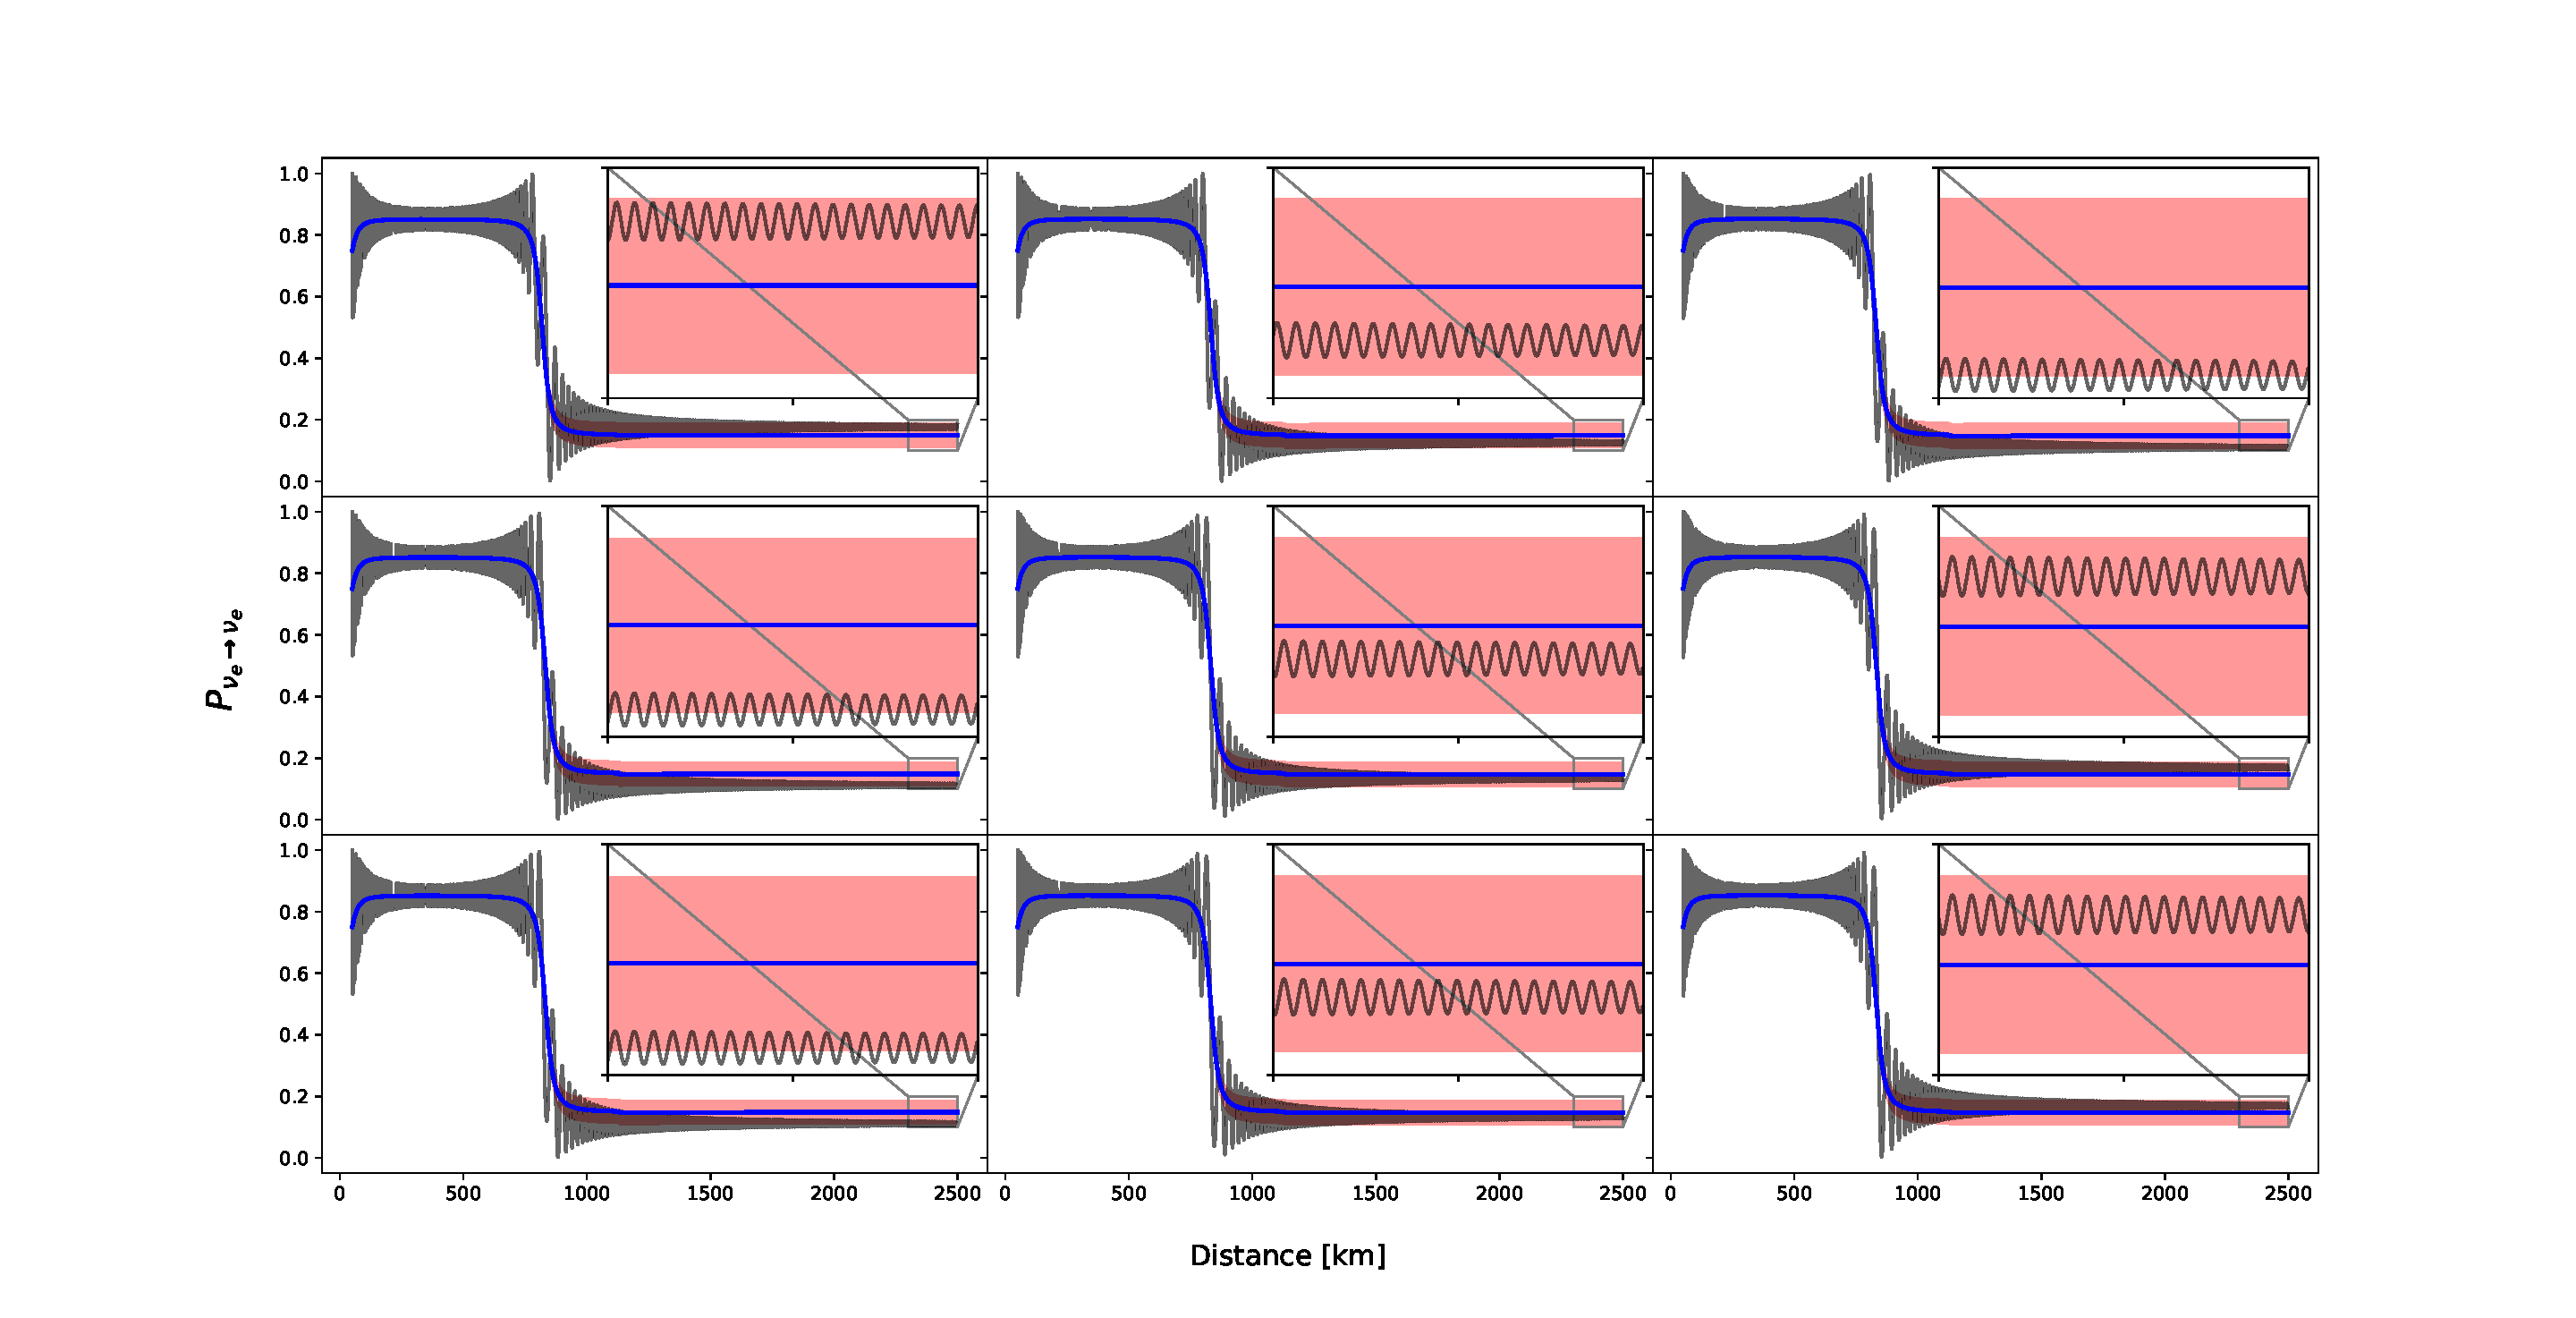
\includegraphics[width=1\textwidth]{figures/theta0expNbB_9x9_10MeV.pdf}
    \caption[theta0expNbB Modelinin, 9 Alt Simülasyonun, $ 10 $ MeV İçin Uzaklığa Karşılık Yaşama Olasılıkları.]{theta0expNbB Modelinin, 9 Alt Simülasyonun, $ 10 $ MeV İçin Uzaklığa Karşılık Yaşama Olasılıkları. Siyah çizgiler simülasyonların sayısal sonuçları, mavi çizgiler analitik öngörü sonuçlarını ve kırmızı aralıklar ise analitik öngörüden sapmaları, yani hatayı göstermektedir. Alt simülasyonların başlangıç koşullarındaki farklar, \ref{tab:oyuncakModel9BasKosul} numaralı tabloda verilmiştir ve sıralama da bu tablodaki gibidir.}
    \label{fig:theta0expNbB_9x9_10MeV}
\end{figure}

Boşluk karışım açısı sıfır olduğunda MSW rezonansı gözükmemesi beklenmektedir. \ref{fig:theta0expNbB_9x9_10MeV} numaralı grafikten de görüldüğü gibi sadece SFP rezonansı meydana gelmektedir.$ 10 $ MeV enerjili nötrinoların SFP rezonansı yaklaşık $830$ km'de meydana gelmiştir ve theta0expNbB simülasyonları için SFP rezonansının LZ geçiş olasılıkları $ 0.003 $ mertebesindedir. Bu geçiş olasılığını veren adyabatisite parametresi ise $ 0.9 $'dur.

Analitik olarak elde ettiğimiz bağıntılar \eqref{eqn:rhoBar_ort} ve \eqref{eqn:rhoBar_hata} numaralı formüller ile verilmiştir. Bu formüllerin, \ref{fig:theta0expNbB_9x9_10MeV} numaralı şekildeki hangi terimlere denk geldiğini açıklayabiliriz. Analitik olarak elde edilen ortalama yoğunluk matris elemanları grafikte mavi çizgi olarak gösterilmiştir. Mavi çizgiler, siyah olan sayısal çözümlerin ortalaması olarak ilerlemektedir. SFP rezonansından sonra da sayısal çözümler ortalama etrafında salınmaya devam etmektedir. Sayısal çözümlerin salınım genlikleri düştüğünde ise ortalama teriminden sapmalar açığa çıkmaktadır. Bu sapmanın tek sebebi rezonansın adyabatik olmamasıdır. Adyabatik olmayan geçişlerde ise fazlar kendisini gösterir. Faz ile orantılı olan analitik sonuçlar ise \eqref{eqn:rhoBar_hata} numaralı bağıntıda verilmiştir. Bu bağıntıda fazların maksimum ve minimum olduğu terim \ref{fig:theta0expNbB_9x9_10MeV} numaralı şekilde kırmızı alan olarak işaretlenmiştir. Yaptığımız çalışmada sayısal sonuçlar ile theta0expNbB adlı model için analitik sonuçlarla tam olarak uyum göstermektedir. Sadece $ R=49.9 $ km, $ r_{mag}=50.1 $ km için olan sonuçlar, \ref{fig:theta0expNbB__R49_9_rmag50_1_10MeV} numaralı grafikte daha yakından gösterilmiştir.

\begin{figure}[hbt!]
    \centering
    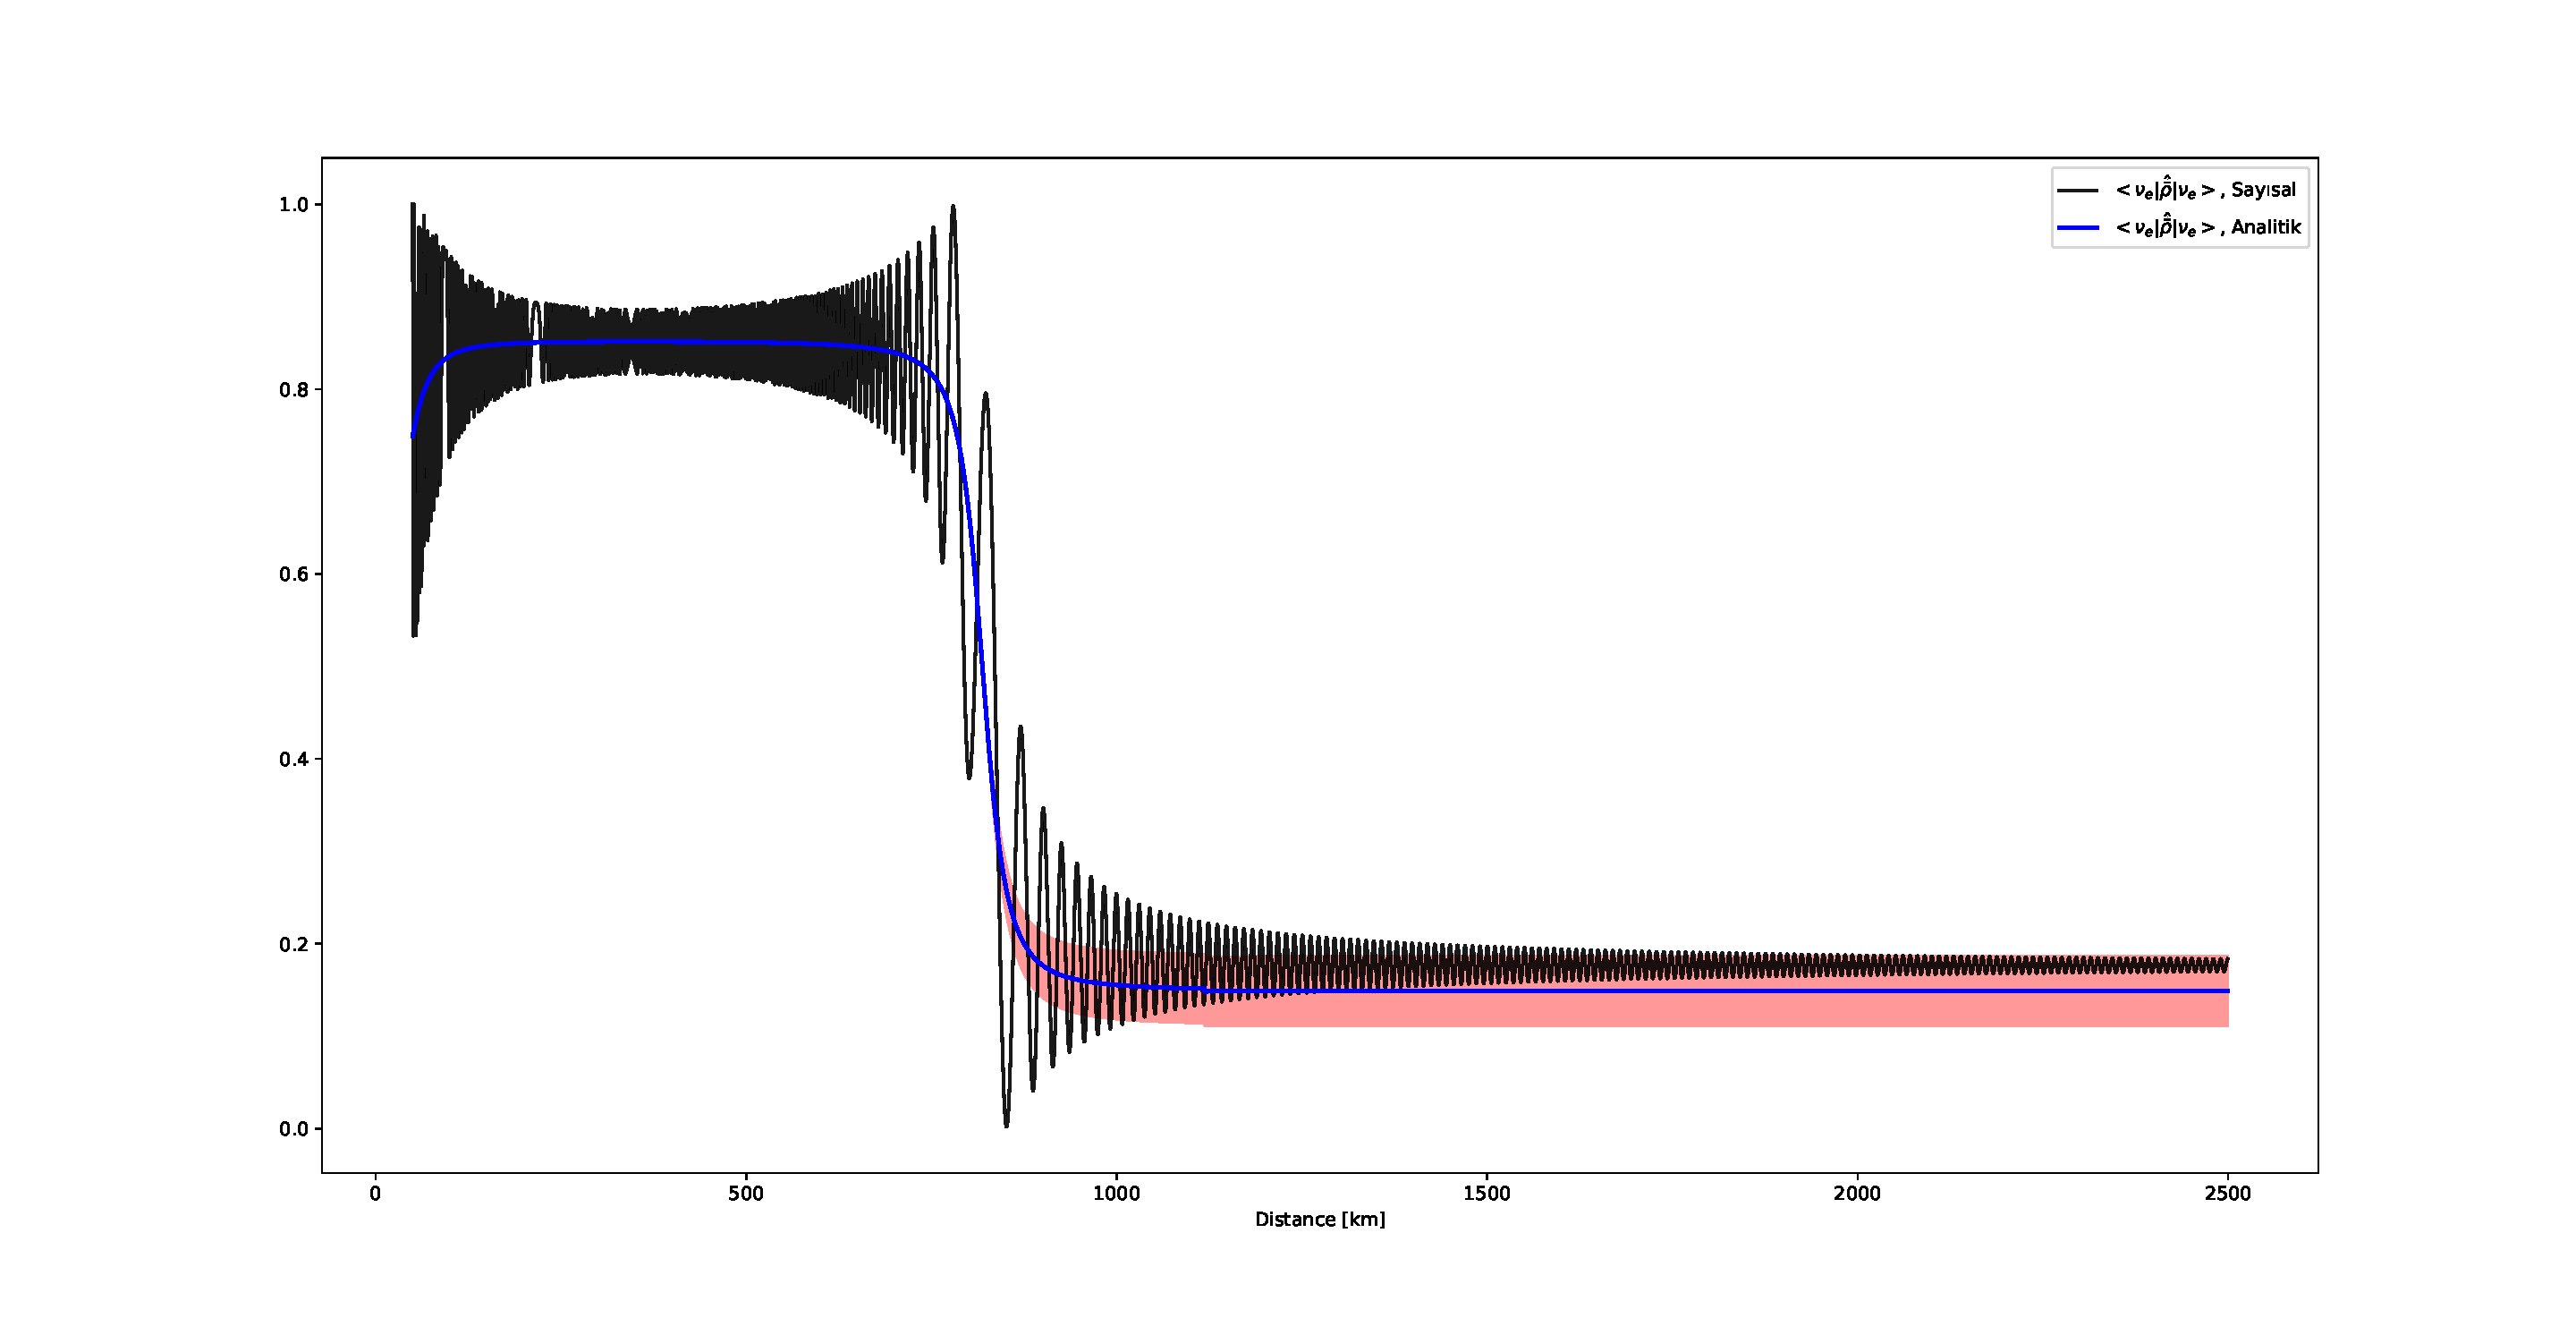
\includegraphics[width=1\textwidth]{figures/theta0expNbB_R49_9_rmag50_1_10MeV.pdf}
    \caption[theta0expNbB Modeli, $ R=49.9 $ km, $ r_{mat}=50.1 $ km simülasyonu ve $ 10 $ MeV İçin Uzaklığa Karşılık Yaşama Olasılıkları]{theta0expNbB Modeli, $ R=49.9 $ km, $ r_{mat}=50.1 $ km simülasyonu ve $ 10 $ MeV İçin Yaşama Olasılıkları}
    \label{fig:theta0expNbB__R49_9_rmag50_1_10MeV}
\end{figure}

theta0expNbB modeli için 9 farklı alt simülasyon yapmamızın sebebi şudur; başlangıç koşullarındaki küçük değişiklikler, fazlardan kaynaklanan sonsuzdaki sayısal çözümlerde küçük değişiklikler meydana getirir. Bu küçük değişikler altında analitik ve sayısal çözümlerin uyumlu olup olmadığına bakılmıştır. Boşluk karışım açısının sıfır olduğu bu simülasyonlar, öngördüğümüz analitik hata aralığı dahilinde doğru sonuçlar vermiştir. 

Elde edilen bu sonuçlar her enerji için geçerlidir. \ref{fig:theta0expNbB_energySpec_theta0_averaged} numaralı grafikte son yaşama olasılıklarının enerjiye göre dağılımı verilmiştir. Bu grafikte mavi çizgiler her enerjideki ortalamanın simülasyon sonundaki değerini göstermektedir. Siyah noktalar ise 9 farklı simülasyonun en son ortalama sayısal değeridir. Yukarıda verilen ve $10$ MeV için geçerli olduğunu gösterdiğimiz analitik ve sayısal sonuç karşılaştırmaları her enerji için geçerlidir. Yani her bir enerji için analitik ve sayısal çözümler tutarlıdır. Düşük enerjide hata aralığının küçülmesi veya yok olmasının sebebi, bu enerjiler için evrimin adyabatik olmasıdır. Adyabatik evrimde $ P_{SFP} $ terimi sıfırdır. Bundan dolayı \eqref{eqn:rhoBar_hata} terimi de sıfır olarak gelecektir. Hata olarak tabir ettiğimiz kırmızı bölge de düşük enerjilerde olmayacaktır.

\begin{figure}[hbt!]
    \centering
    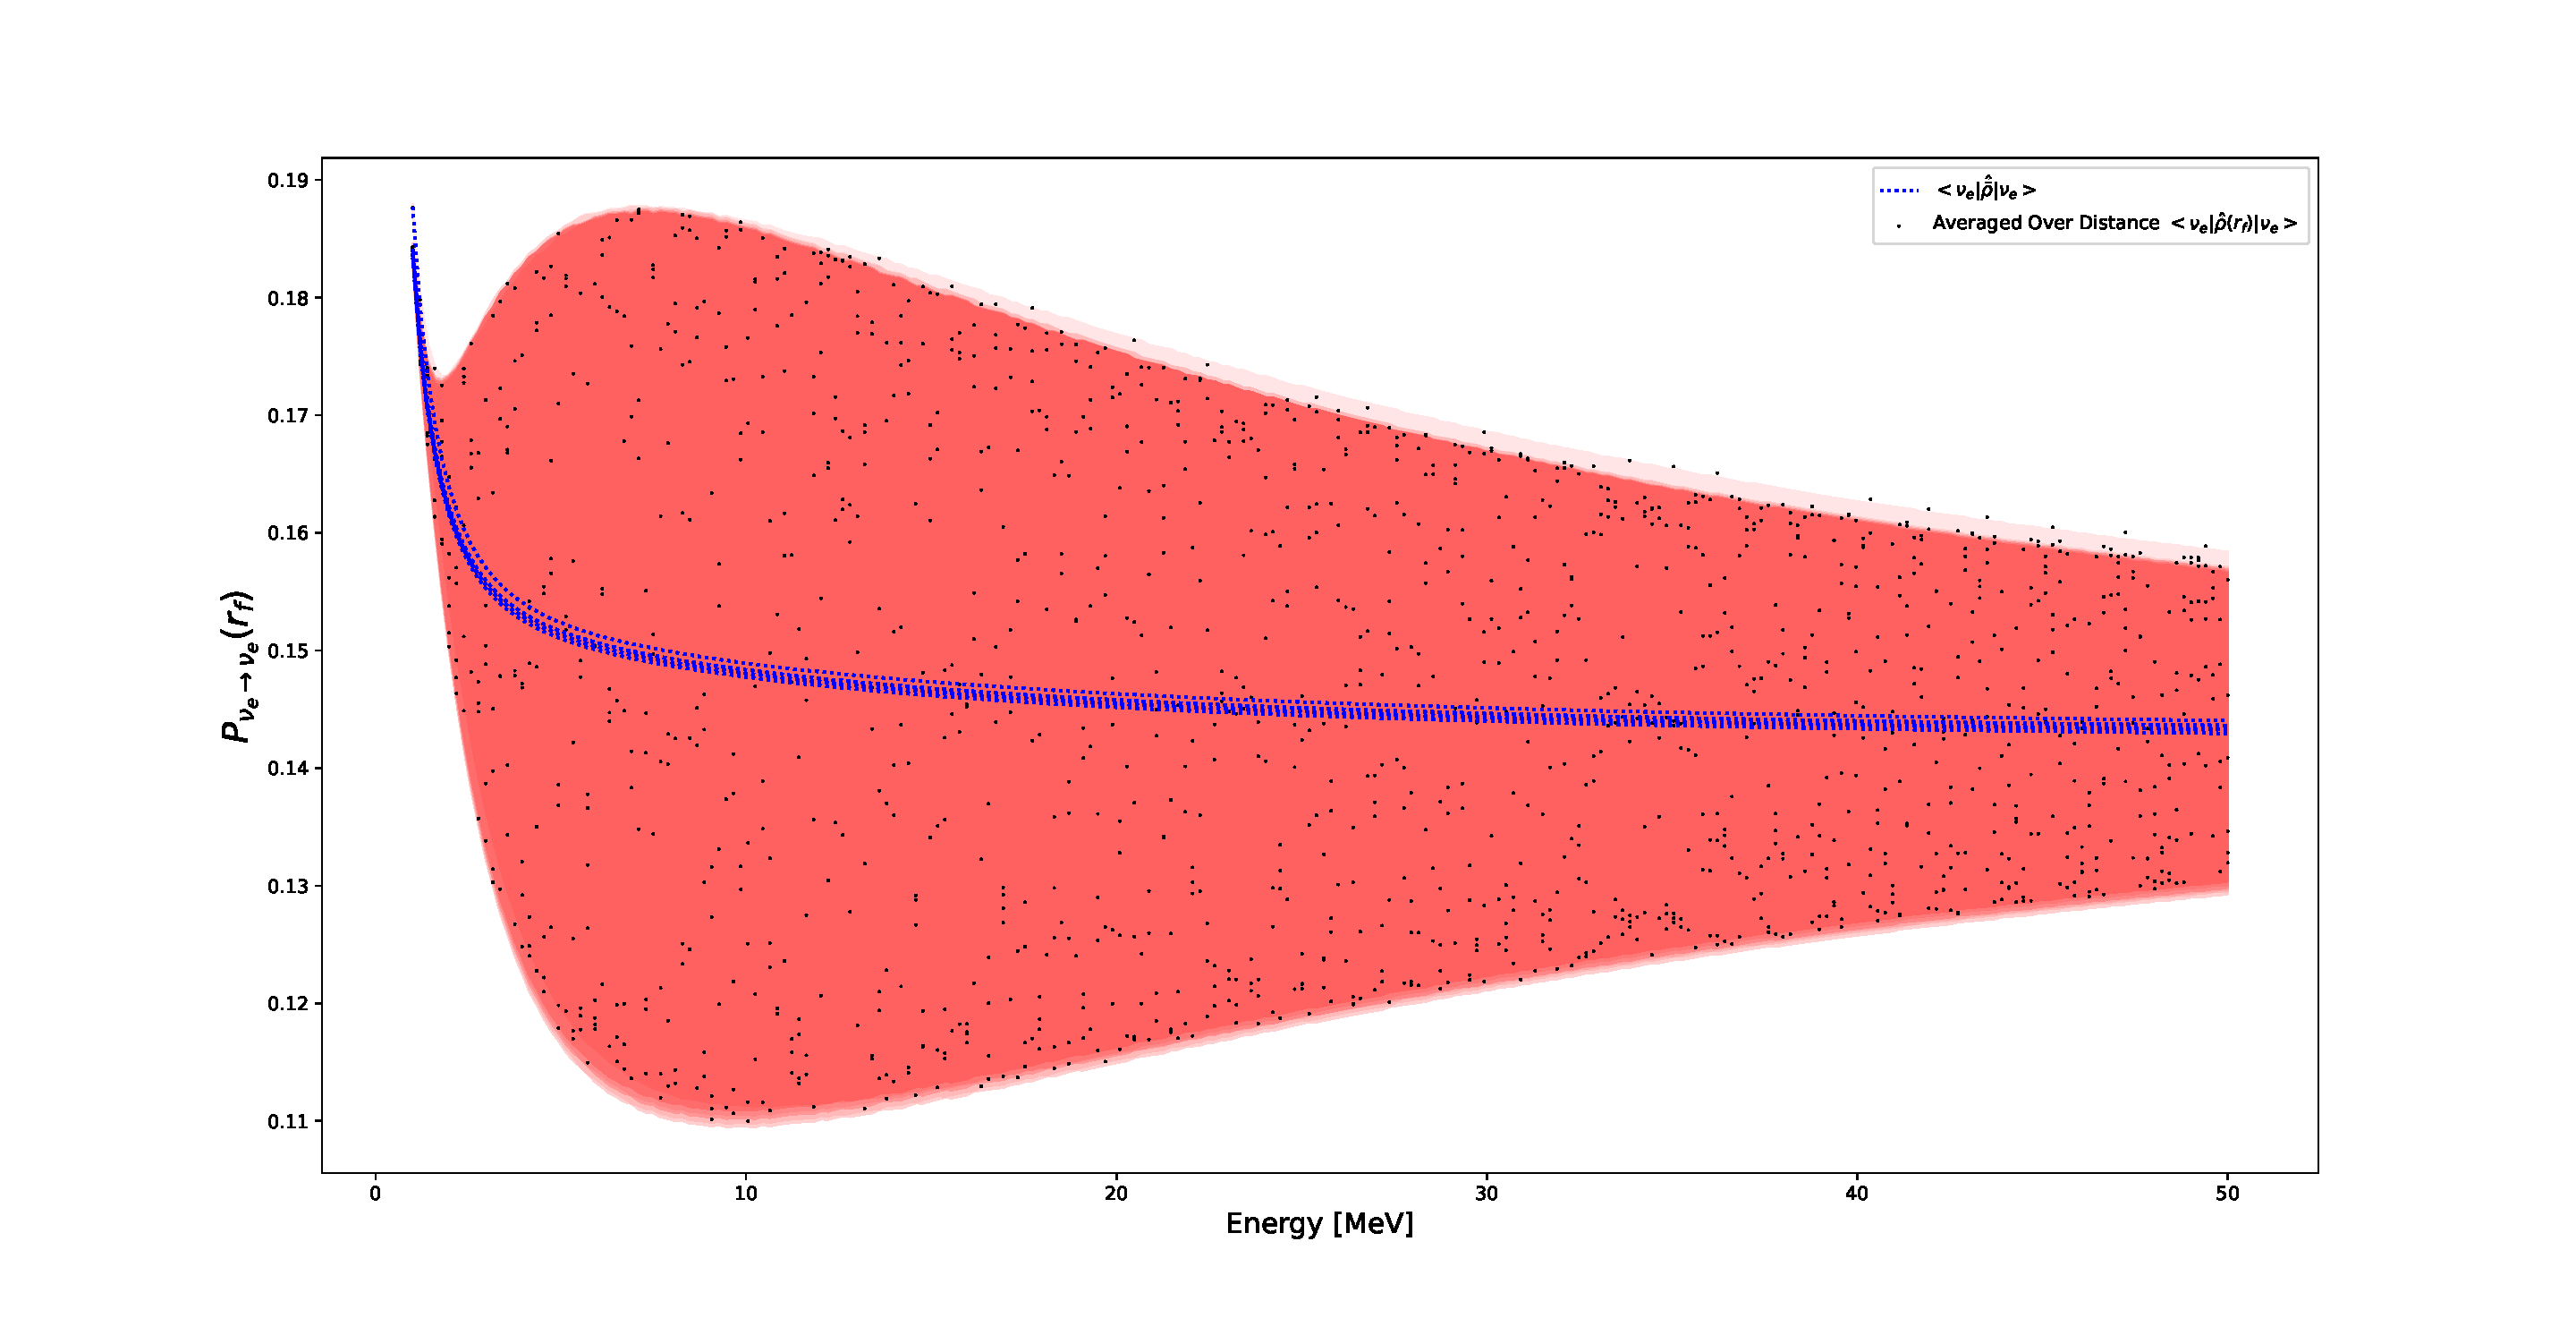
\includegraphics[width=\textwidth]{figures/theta0expNbB_energySpec_theta0_averaged.pdf}
    \caption[theta0expNbB Modeli, 9 simülasyonun Enerjiye Karşılık Yaşama Olasılıkları]{theta0expNbB Modeli, 9 simülasyonun Enerjiye Karşılık Yaşama Olasılıkları. Her siyah nokta, sayısal sonuçların son birkaç kilometredeki ortalamasıdır.}
    \label{fig:theta0expNbB_energySpec_theta0_averaged}
\end{figure}

Fazların çeşni evrimine olan etkisi de \ref{fig:theta0expNbB_energySpec_theta0_averaged} numaralı grafikten gözükmektedir. Her enerji için yapılan 9 simülasyon sonucunda sayısal sonuçlar belli bir noktada olmayıp bir aralık arasında "rastgele" dağılmaktadır. LZ geçiş olasılığından kaynaklanan hata aralığı, $ 10 $ MeV civarında en yüksek değere ulaşmıştır. Bu sonuç, Dünya'dan yapılacak olan nötrino algıç (detect) deneylerinden SN modelleri oluşturulmasında önemli yer tutar.

\textbf{theta014expNbB} adlı simülasyonun analitik ve sayısal sonuçları, karşılaştırılmalı olarak \ref{fig:theta014expNbB_9x9_10MeV} numaralı şekilde verilmiştir.

\begin{figure}[hbt!]
    \centering
    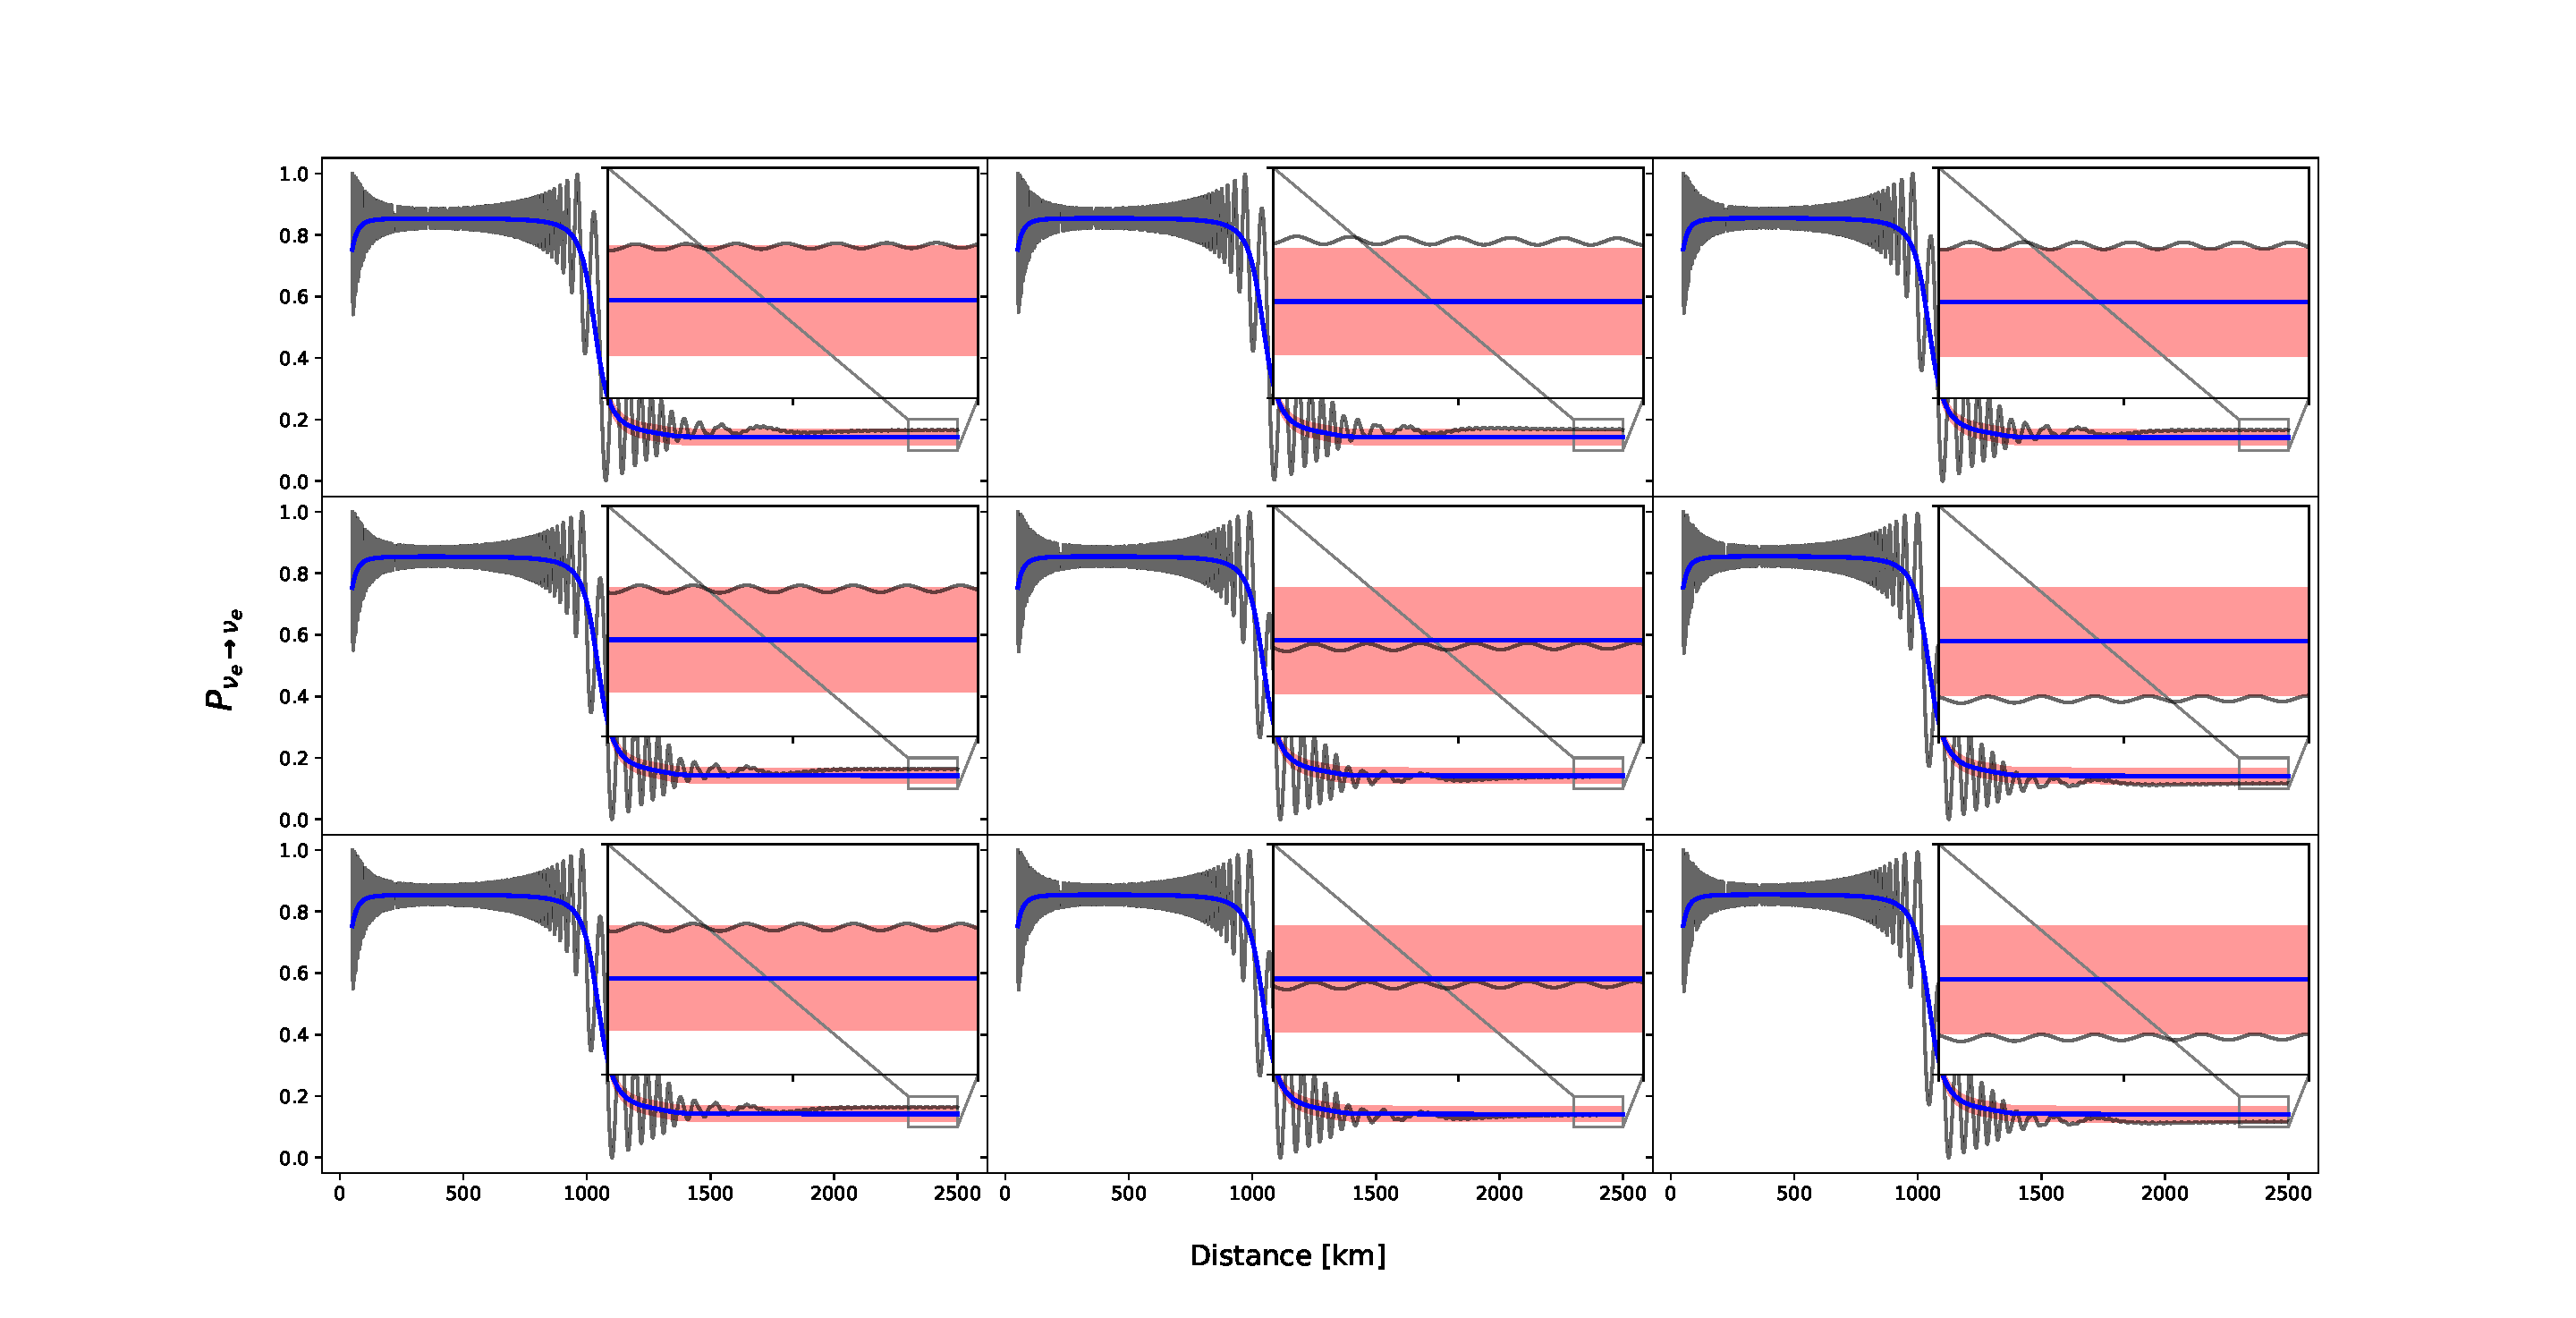
\includegraphics[width=\textwidth]{figures/theta014expNbB_9x9_10MeV.pdf}
    \caption[theta014expNbB Modelinin, 9 Alt Simülasyonun, $ 10 $ MeV İçin Uzaklığa Karşılık Yaşama Olasılıkları]{theta014expNbB Modelinin, 9 Alt Simülasyonun, $ 10 $ MeV İçin Uzaklığa Karşılık Yaşama Olasılıkları. Siyah çizgiler simülasyonların sayısal sonuçları, mavi çizgiler analitik öngörü sonuçlarını ve kırmızı aralıklar ise analitik öngörüden sapmaları, yani hata aralığını göstermektedir. $ 10 $ MeV enerjisi için, ($ R=49.90 $, $ r_{Mag}=50.05 $), ($ R= 49.90$, $ r_{Mag}=50 $), ($ R= 49.95$, $ r_{Mag}=50 $) ve ($ R= 50.00$, $ r_{Mag}=50 $) başlangıç koşullarına sahip olan simülasyon sonuçları analitik öngörü ile uyuşmamaktadır.}
    \label{fig:theta014expNbB_9x9_10MeV}
\end{figure}

Karışım açısının sıfır olmadığı durumda SFP rezonansına ek olarak MSW rezonansı da gerçekleşecektir. \ref{fig:theta014expNbB_9x9_10MeV} numaralı şekil $ 10 $ MeV enerjili nötrinolar için çizilmiş olup SFP rezonansı yaklaşık $840$ km'de meydana gelmiştir. MSW rezonansı ise $ 1270 $ km civarında meydana gelmektedir. theta014expNbB simülasyonları için SFP LZ geçiş olasılıkları $ 0.003 $ mertebesinde ve MSW geçiş olasılıkları $ 10^{-14} $ mertebesindedir. Bu geçiş olasılığını veren adyabatisite parametresi ise SFP için $ 0.9 $, MSW için $ 4.8 $ mertebesindedir.

theta0expNbB modelinden farklı olarak theta014expNbB modelinde, analitik olarak elde ettiğimiz bağıntılar \eqref{eqn:rhoBar_ort} \eqref{eqn:rhoBar_hata} numaralı formüller ile bazı sayısal çözümlerin uyuşmadığı görülmektedir. Bu MSW ve SFP rezonanslarının iki ayrı $ 2\times2 $ sistem olarak ele alınmasından kaynaklanan bir hatadır diyebiliriz. Öncelikle bu durumun $ 10 $ MeV ile sınırlı olmadığını, tüm enerjilerde bir miktar uyumsuzluk olduğunu söylemek gerekir. \ref{fig:theta014expNbB_energySpec_theta0_averaged} numaralı grafikten de açıkça görüldüğü gibi siyah nokta ile gösterilen sayısal çözümler kırmızı ile verilen hata aralığın dışına çıkmıştır. Hatta yüksek enerjili nötrinolarda fark büyümektedir.

\begin{figure}[hbt!]
    \centering
    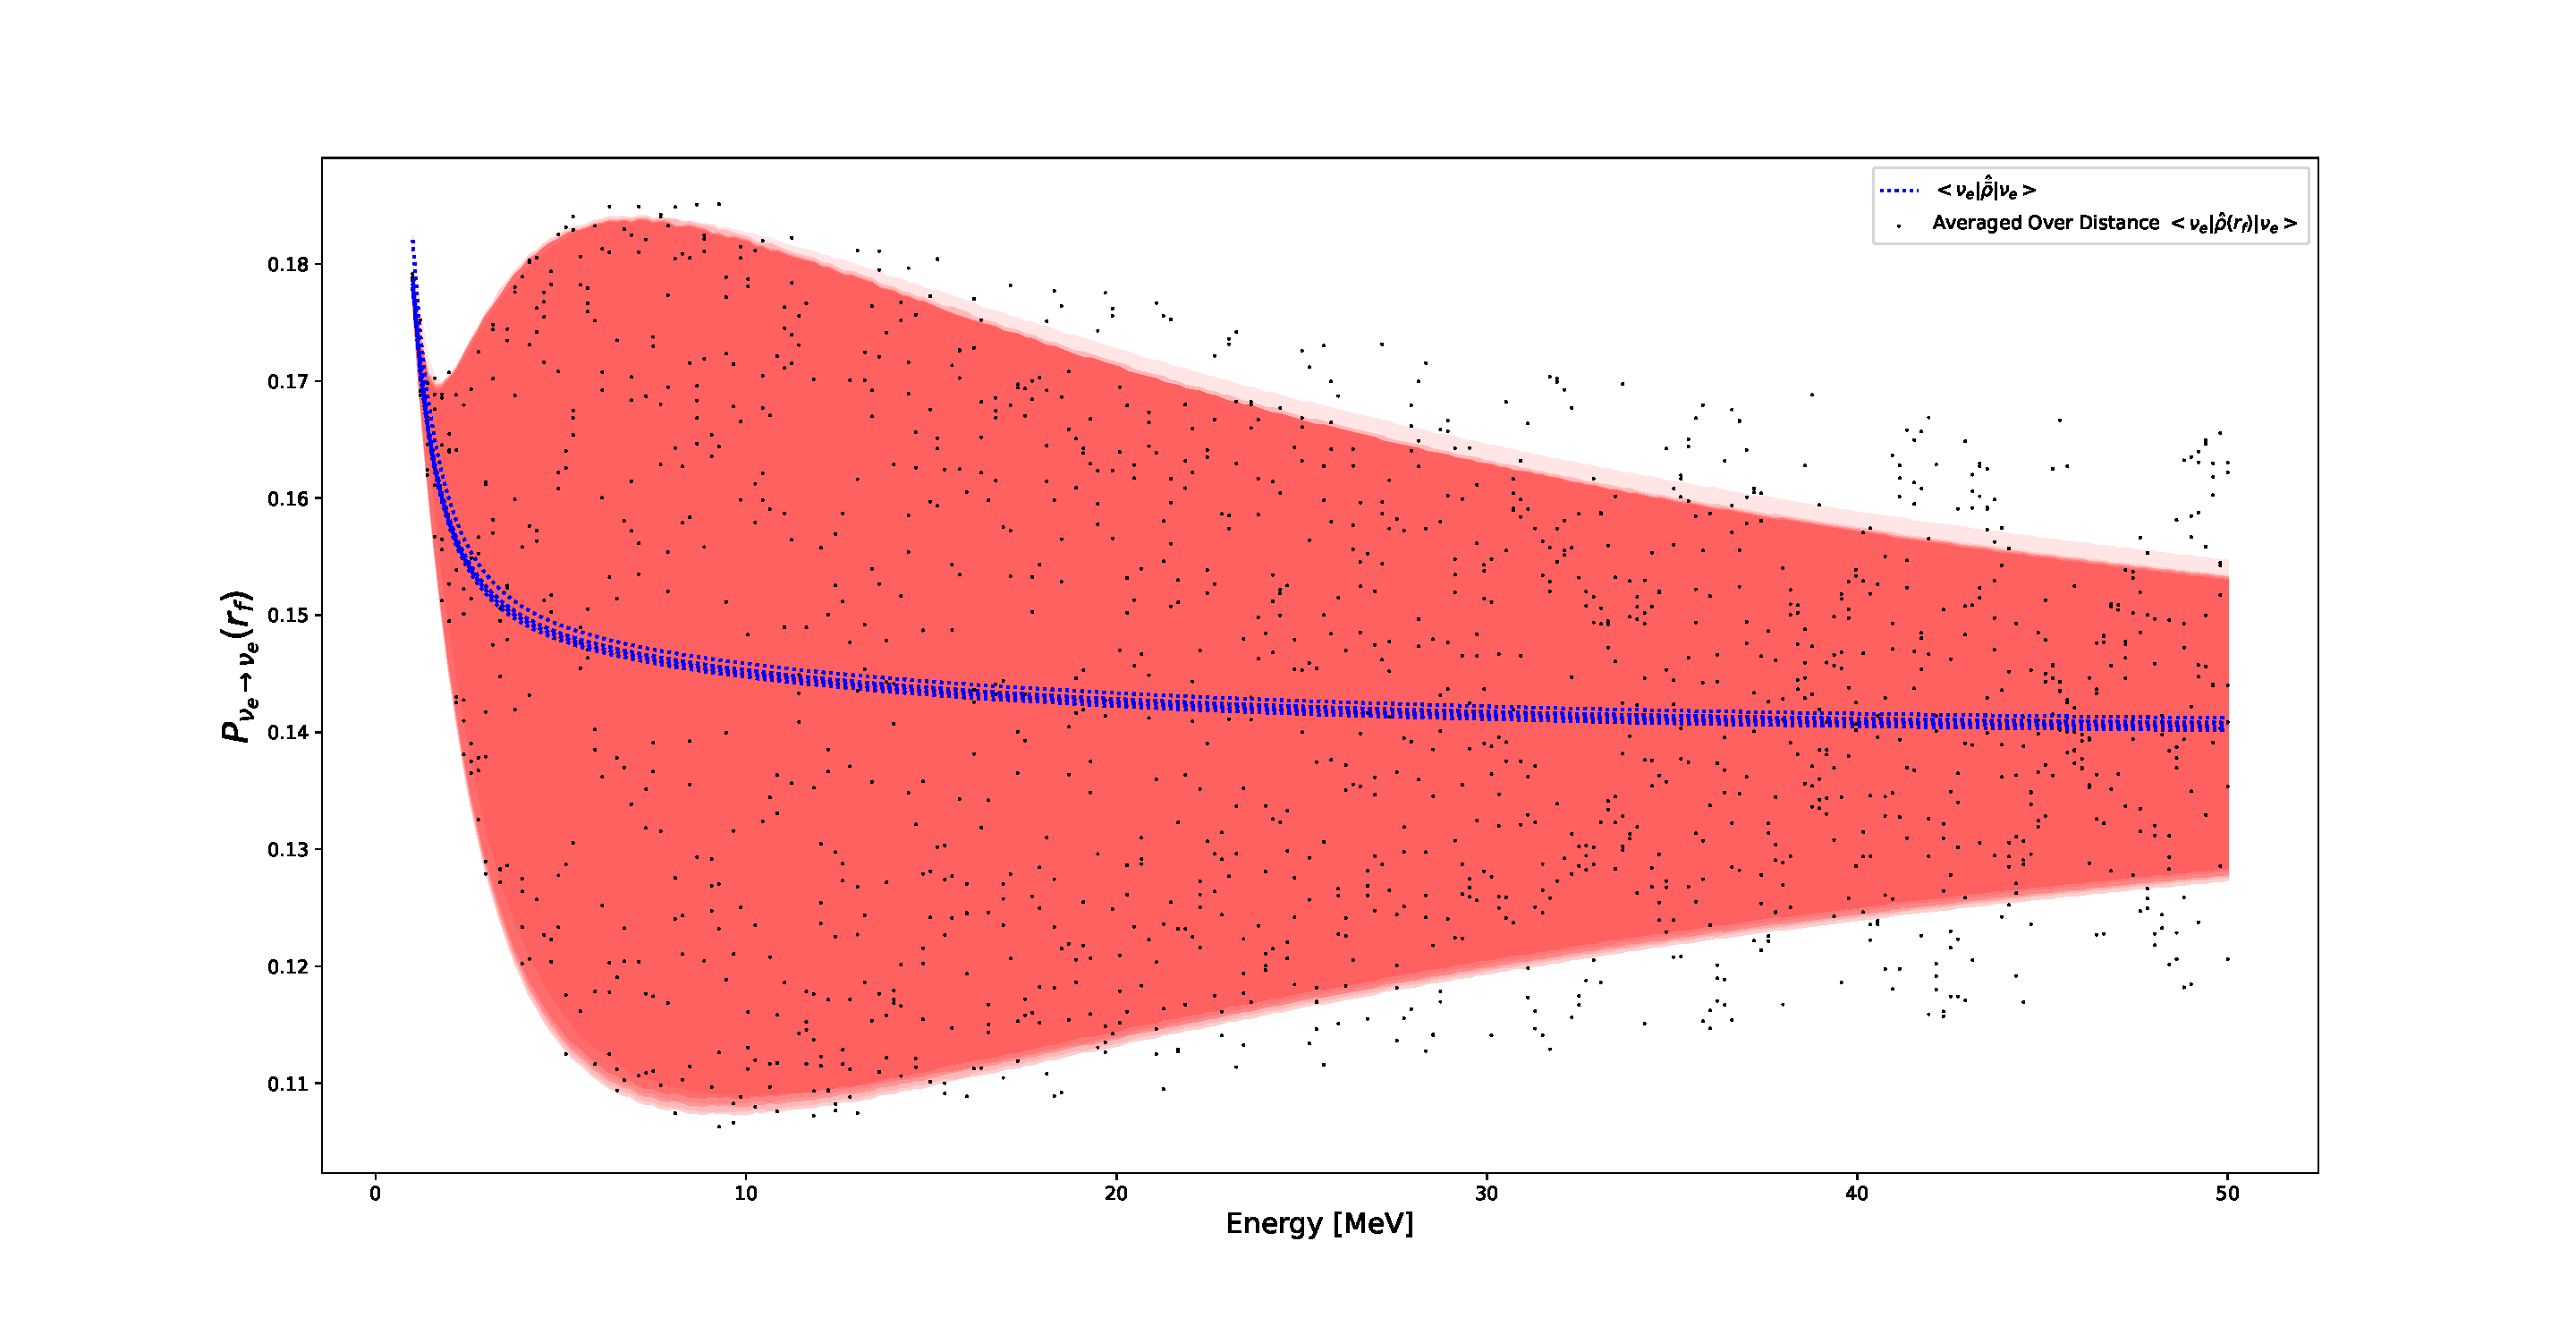
\includegraphics[width=\textwidth]{figures/theta014expNbB_energySpec_theta0_averaged.pdf}
    \caption[theta014expNbB Modeli, 9 simülasyonun Enerjiye Karşılık Yaşama Olasılıkları]{theta014expNbB Modeli,9 simülasyonun Enerjiye Karşılık Yaşama Olasılıkları. Her siyah nokta, sayısal sonuçların son birkaç kilometredeki ortalamasıdır. Boşluk karışım açısının sıfırdan farklı olması durumunda, analitik öngörü/sayısal sonuç uyumsuzluğu görülmektedir. Uyumsuzluk, yüksek enerjilerde daha belirgin hale gelmektedir.}
    \label{fig:theta014expNbB_energySpec_theta0_averaged}
\end{figure}

Eğer nötrino çeşni evriminde, bir rezonans tamamlanmadan sonraki rezonansa girer ise analitik olarak hesapladığımız ortalama yoğunluk matrisi terimi yani \eqref{eqn:rhoBar_rhoSal} numaralı denklem tam olarak doğru sonucu vermez. Bunun ilk sebebi adyabatik olmayan geçişleri veren $ A_{ij} $ terimi MSW ve SFP olmak üzere iki ayrı matrisin çarpımı olarak yazılamayacaktır. \eqref{eqn:rhoBar_hata} numaralı denklemde hata terimi türetilirken $ A_{LZ} = A_{SFP} \times A_{MSW} $ şeklinde yazıldığından dolayı elde ettiğimiz analitik öngörü formülleri tam doğru değildir. İkinci olarak ise SFP rezonansı için yazılan ve LZ geçiş olasılığını veren \eqref{eqn:LZOlasilik} numaralı formül geçerli olmayacaktır. Bunun nedeni SFP rezonansının adyabatisitesi, rezonans bölgesinde hesaplanırken efektif 2 çeşniye düşülmüştür. Bu da, rezonans bölgesinde $ \Delta \sin(2\theta) $ teriminin $ \mu B $ teriminden çok çok büyük olması varsayımında geçerlidir. theta014expNbB modelinde, $ 10 $ MeV enerjili nötrinoların tam SFP rezonansına girdiği noktada toplam Hamiltonyen'in sayısal değeri aşağıdaki gibidir. 
\begin{equation}
    H(r=840 \text{ km}) = \mqty(1.4 & -0.1 & 0 & 0.1\\ -0.1 & -2.0 & -0.1 & 0\\ 0 & -0.1 & -0.7 & -0.1\\ 0.1 & 0 & -0.1 & 1.4) ~~\text{[km}^{-1}\text{]} \text{ .}
\end{equation}
Yukarıdaki denklemden de görüleceği üzere Hamiltonyen matrisinin 12 elemanının değeri ile 14 elemanın değeri aynıdır. Bu da SFP rezonansının adyabatisite değerini bulmak için yaptığımız $ 2\times2 $ çeşni indirgenmesini olanaksız kılar. Budan dolayı $ P_{SFP} $, yanlış bir değer alır.

Analitik sonuçlar ile sayısal sonuçların uyuşmamasını daha ayrıntılı inceleyebilmemiz için iki rezonans noktası etrafındaki efektif karışım açısının sinüsünün karesine bakmak gerekmektedir, çünkü salınım ortalaması alınmış elektron yaşama olasılıkları, $ \sin^{2}(2\theta) $ ile orantılıdır \cite{Kuo:1989qe}. Buradaki $\theta $ terimi, madde etkileşimleri için $ \theta_{M} $ şeklinde, hem madde hem de elektromanyetik etkileşimler için $ \theta_{EM} $ şeklinde gelir. $ \sin^{2}(2\theta_{M}) $ ve $ \sin^{2}(2\theta_{EM}) $ terimlerinin uzaklıkla değişiminde, bu terimlerin ilgili rezonanslarda $ 1 $ değeri alacağı bilinmektedir, çünkü rezonans değerlerinde efektif karışım açısı $ \pi/4 $ değerine yaklaşacaktır. 

Efektif karışım açısının sinüsünün karesinin uzaklıkla değişimi \ref{fig:theta014expNbB_sin2_thetaM_thetaEM_dist10MeV} numaralı şekilde verilmiştir. Bu grafikte $ 40 $ MeV enerjili nötrinolar, SFP rezonansından çıkamadan MSW rezonansına girdiği gözükmektedir. Rezonansların üst üste binmesini farklı başlangıç baryon yoğunluklarına bakarak karşılaştırabiliriz. \ref{fig:theta014expNbB_sin2_thetaM_thetaEM_dist10MeV} numaralı şeklindeki en üstteki şekil, $ n_{0}=10^{6} $ g/cm$ ^{3} $ için yapılmış simülasyon sonucudur. Bu değerden daha büyük değerler alınırsa, ÇÇSN'nın daha erken dönemlerine gidilmiş olur. $ n_{0}=2.3\times 10^{6} $ g/cm$ ^{3} $ değeri $ t=3 $ s için olan evreye ve $ n_{0}=1.8\times 10^{7} $ g/cm$ ^{3} $ değeri $ t=1 $ s için olan evreye denk gelmektedir. Bunlar için analitik öngörümüzü test edebiliriz.

\begin{figure}[hbt!]
    \centering
    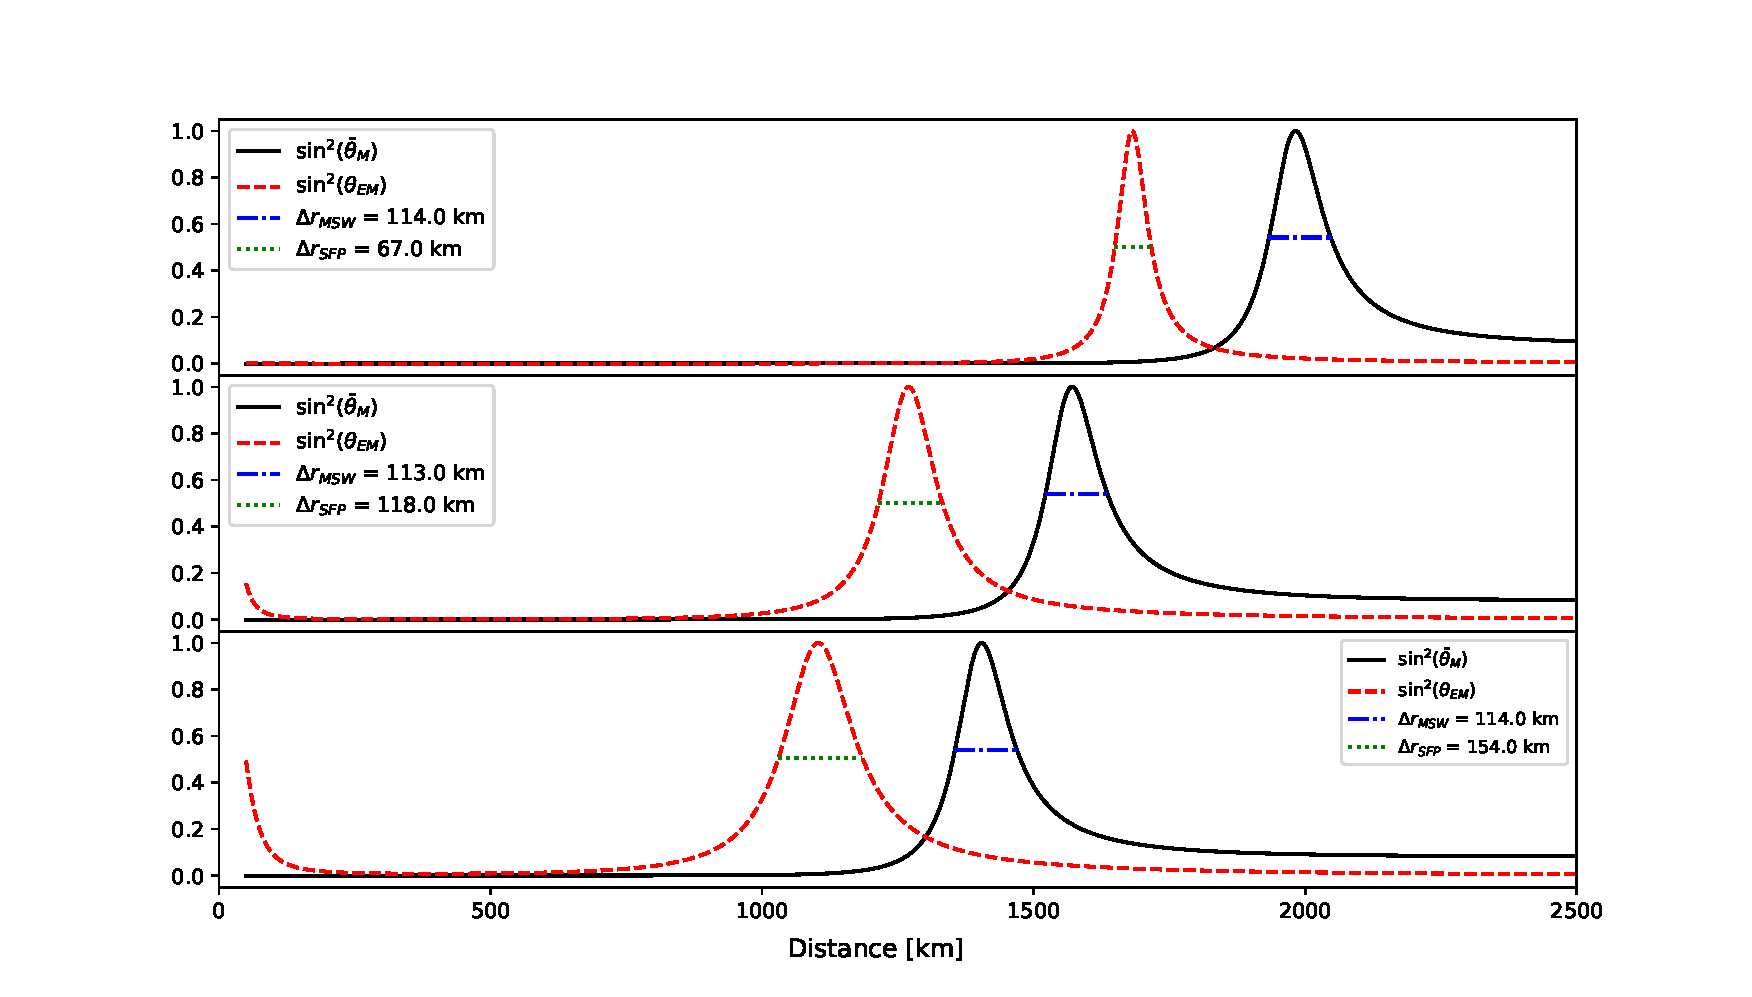
\includegraphics[width=\textwidth]{figures/widthCompare3x1_40MeV_IH_t135s.pdf}
    \caption[theta014expNbB Modelinde Rezonansların Birbirine Yakınlığı]{theta014expNbB Modelinde Rezonansların Birbirine Yakınlığı. $ \Delta r_{MSW} $ uzaklığı ile $ \Delta r_{SFP} $ uzaklığının baryon yoğunluğunun başlangıçtaki değerine göre değişimi gösterilmiştir. Şekiller, yukarıdan aşağı $ t=1 $ s, $ t=3 $ s ve $ t=5 $ s için kullanılan ÇÇSN baryon profilleri baz alınmıştır.}
    \label{fig:theta014expNbB_sin2_thetaM_thetaEM_dist10MeV}
\end{figure}

Rezonansların birbirine yakınlığı ve öngörülerimizin çalıştığı aralığı belirlemek için $ \sin^{2}(2\theta_{M}) $ ve $ \sin^{2}(2\theta_{EM}) $ terimlerinin eksponansiyel profil için analitik değerlerini hesaplamalıyız. $ \sin^{2}(2\theta) $ fonksiyonu neredeyse Gausyen bir dağılım verdiği için dağılımın yarım maksimumdaki yarım genişlik (YMYG), (half width at half maksimum, HWHM) değerleri anlamlı olacaktır. \ref{fig:theta014expNbB_sin2_thetaM_thetaEM_dist10MeV} numaralı grafikte yazan $ \Delta r_{MSW} $ ve $ \Delta r_{SFP} $ değerleri YMYG değerinin iki katıdır ve grafik üzerinden hesaplanmıştır. Bu değeri analitik olarak hesaplamak da mümkündür. $\sin^{2}(2\theta_{M}) $ teriminin yarı maksimum olduğu uzaklık, $\Delta r_{MSW}$, ifadenin $ 0.5 $'e eşit olduğu değerde olacaktır.
\begin{align}
    \sin^{2}(2\theta_{M}(\Delta r_{MSW}) ) = 0.5 = \frac{1}{1+\frac{\Delta c_{2\theta} - V_{CC}(\Delta r_{MSW})/2}{\Delta s_{2\theta}}} \text{ .}
\end{align}
Burada $ \Delta r_{MSW} $ uzaklığı, maksimum değerinin etrafında, iki farklı değerde olacaktır. Bu uzaklıklar, $ n_{b}(r) = n_{0}\exp(-r/r_{mat}) $ profili için aşağıdaki değerleri alır.
\begin{equation}
    r^{MSW}_{hm1}, r^{MSW}_{hm2} = (-r_{mat})\ln(\frac{1}{n_{0}}\frac{\Delta c_{2\theta} \pm \Delta s_{2\theta}}{\sqrt{2} G_{F} Y_{e}/2}) \text{ .}
\end{equation}
MSW rezonansının meydana geldiği noktadaki yarım genişlik $ r^{MSW}_{hw} $, MSW rezonansının kaç kilometre boyunca meydana geldiğini betimleyen bir büyüklük olarak karşımıza çıkar ve bu değer aşağıdaki gibi tanımlanır.
\begin{align} \label{eqn:rMSW_hw}
    \nonumber \Delta r_{MSW}/2 =& \abs{r^{MSW}_{hm1}- r^{MSW}_{hm2}}/2 \text{ ,}\\
    =& \frac{-r_{mat}}{2} \ln(\frac{c_{2\theta} - s_{2\theta}}{c_{2\theta} + s_{2\theta}}) \text{ .}
\end{align}
Bu ifadeden de görüleceği üzere, MSW rezonansının genişliği enerjiden, kütle kare farkından ve baryon yoğunluğunun başlangıçtaki değerinden bağımsızdır. 

Benzer işlemleri SFP rezonansı için de yapabiliriz. Manyetik alanın $ B(r) = B_{0}(50 \text{ km}/r)^{2} $ şeklinde alınacaktır. SFP rezonansının gerçekleştiği yarı maksimum uzaklıkları aşağıdaki denklemlerin çözümü ile verilir.
\begin{align}
    \Delta c_{2\theta} - \frac{2Y_{e}-1}{2}\sqrt{2}G_{F}n_{0}e^{-\Delta r_{SFP}/r_{mat}}\pm \mu B_{0}(50 \text{ km}/\Delta r_{SFP})^{2} = 0\text{ .}
\end{align}
Bu denklemin $ \Delta r_{SFP} $ için çözümü yoktur. Bunun yerine rezonans bölgesinde manyetik alanın neredeyse sabit ve $ B_{1} $ değeri aldığını varsayacağız. Bu yaklaşıklık altında yarım genişlik $ \Delta r_{SFP}/2 $ değeri aşağıdaki gibi hesaplanır.
\begin{equation}\label{eqn:rSFP_hw}
    \Delta r_{SFP}/2 = \frac{-r_{mat}}{2} \ln(\frac{\Delta c_{2\theta}-\mu B_{1}}{\Delta c_{2\theta}+\mu B_{1}})\text{ .}
\end{equation}
Bu ifade, $ r^{MSW}_{hw} $ genişliğinden farklı olarak enerjiye, kütle kare farkına ve manyetik alana da bağlıdır. \eqref{eqn:rMSW_hw} ve \eqref{eqn:rSFP_hw} numaralı denklemlerden elde edilen YMYG ile \ref{fig:theta014expNbB_sin2_thetaM_thetaEM_dist10MeV} numaralı şekilden elde edilen YMYG değeri farklı olacaktır. Örneğin karışma açısı büyüdükçe, $ \sin^{2}(2\theta_{M}) $ ifadesinin grafikten elde edilen yarı maksimumun değeri $ 0.5 $'ten uzaklaşacaktır. Ayrıca \ref{fig:theta014expNbB_sin2_thetaM_thetaEM_dist10MeV} numaralı şekilden MSW rezonansının YMYG değeri, $ n_{0} $'dan bağımsız olduğu gözükmektedir.

Rezonansların birbirine ne kadar yakın olduklarını sayısal bir değer tanımlayarak belirleyebiliriz. Bunun için \ref{fig:theta014expNbB_sin2_thetaM_thetaEM_dist10MeV} numaralı şekildeki Gausyen dağılımın YMYG değeri bize bir fikir verecektir. \cite{Smirnov:2003da} numaralı kaynağın 6 numaralı şeklinde, rezonansın başlangıç ve bitiş noktaları rezonansın meydana geldiği noktadan yaklaşık $3$ adet YMYG değeri kadar uzaklarda "bittiği" anlaşılmaktadır. Eğer, rezonansların birbirlerine olan uzaklığının, yarı uzaklık toplamlarına oranı sıfıra yaklaşırsa rezonanslar üst üste geliyor demektir. \ref{fig:theta014expNbB_sin2_thetaM_thetaEM_dist10MeV} numaralı grafikteki değerler için bu oranları yazabiliriz.
\begin{align}\label{eqn:resonansYakinlasmaOranı}
    \eval{\frac{\abs{r^{SFP} - r^{MSW}}}{r^{SFP}_{hw}+r^{MSW}_{hw}}}_{t=1,3,5 \text{ s}} = 3.31\text{, } 2.60\text{, } 2.24 \text{ .}
\end{align}
Yukarıdaki değerlere bakınca, ÇÇSN erken evrelerinde (başlangıç baryon yoğunluk değeri arttıkça) rezonansların birbirinden daha ayrı olduğunu söyleyebiliriz. ÇÇSN evriminde zaman ilerledikçe rezonanslar birbirine yaklaşmaktadır. Rezonansların birbirine yaklaşması üç çeşni etkilerinin ortaya çıkması anlamına da gelir.

Çeşni evrimindeki üç çeşni etkilerini başka bir parametre ile de görmek mümkündür. SFP rezonansının başladığı sırada, \eqref{eqn:Hamiltonyen_withGamma} numaralı Hamiltonyen'i üç çeşniye indirgeyelim. Bu Hamiltonyen, madde tabanında yazıldığı için seçeceğimiz üç terim, başlangıç koşullarına bağlıdır. Bizim notasyonumuza göre, ters hiyerarşi ve $ Y<0.5 $ başlangıç koşulları için indirgenmesi gereken terimler $ \omega_{1,2,4} $ ve bunlarla alakalı olan terimler olacaktır.

\begin{equation}
    H_{3\times3} = \mqty(\omega_{1} & \mu B \sin\gamma & \mu B \cos \gamma \\ \mu B \sin\gamma & \omega_{2} & \mu B \sin \gamma \\ \mu B \cos \gamma & \mu B \sin\gamma & \omega_{4}) \text{ .}
\end{equation}

Salınım etkilerinin olmadığı durumlarda, $ \theta=0 $, efektif madde karışım açı farkı $ \gamma=0 $ olur. Bu durumda geçişler sadece $ \omega_{1} $ ile $ \omega_{4} $ arasında olacaktır. Başlangıçta, birinci öz durum çoğunlukla elektron, dördüncü öz durum çoğunlukla anti $x$ çeşnisi olduğu düşünüldüğünde, bu geçişler SFP rezonansına sebep olacaktır.

Boşluk salınım açısının sıfırdan farklı olduğu durumda ise SFP rezonansı sırasında köşegen olmayan terimler sıfır olmayacak. Yani $ \mu B \sin \gamma \ne 0 $ şeklinde olacaktır. Bir diğer taraftan, SFP rezonansının meydana geldiği uzaklıkta $ \omega_{1}-\omega_{4} $ neredeyse sıfır olacaktır. Bu noktadaki üç çeşniye indirgenmiş Hamiltonyen'i tekrar yazalım. Hamiltonyen'i yazarken $ \omega_{4} $ ile birim matris çarpımını Hamiltonyen'den çıkaralım. 
\begin{equation}
    H_{3\times3}(r_{SFP}) = \mqty(0 & \mu B \sin\gamma & \mu B \cos \gamma \\ \mu B \sin\gamma & \omega_{2}(r_{SFP})-\omega_{4}(r_{SFP}) & \mu B \sin \gamma \\ \mu B \cos \gamma & \mu B \sin\gamma & 0) \text{ .}
\end{equation}
Sistem SFP rezonansına girerken, özdurum geçişleri sadece $ \omega_{1} $ ile $ \omega_{4} $ arasında olmayacaktır. $ \mu B \sin \gamma $ teriminden kaynaklı $ \omega_{2} $ ile $ \omega_{4} $ arasında da olacaktır. Bu nedenle, iki çeşniye indirgenerek elde edilen tüm parametreler düzgün çalışmaz. 

Yukarıda bahsedilen, özdurumlar arasındaki bu \emph{sızma} (leaking) olayının büyüklüğünü, sızma parametresi $ L $ terimini tanımlayarak belirleyebiliriz.
\begin{equation}
    L = \eval{\frac{\mu B \sin \gamma}{\omega_{i}-\omega_{j}}}_{r_{SFP}}
\end{equation}

theta014expNbB başlangıç koşulları kullanıldığında $ i,j = 2,4 $ olacaktır. \textit{Sızma parametresi ne kadar küçük olursa üç çeşni etkileri o kadar az olur.} theta014expNbB simülasyonu için $ L $ parametresi $ 20 $ civarındadır. Sızma parametresi $ 5 $ civarında iken üç çeşni etikleri çok küçüktür ve öngörü/simülasyon sonuçları tam olarak uyumlu çıkar. Sızma parametresi için söylenecek son söz ise boşluk karışım açısı $ \theta $ arttığında veya başlangıçtaki madde yoğunluğu azaldığında $ L $ değeri büyüyecektir. 

Sonuç olarak \eqref{eqn:rhoBar_ort} ve \eqref{eqn:rhoBar_hata} numaralı denklemler ancak ve ancak \eqref{eqn:resonansYakinlasmaOranı} numaralı bağıntıda verilen oran $ 3 $'ten büyük ise veya $ L \sim 5$ olduğunda kullanılabilir. Elde ettiğimiz bu iki koşul birbiriyle ilişkilidir. 

Elde ettiğimiz öngörüleri ve geçerli olduğu başlangıç koşulları kullanarak ÇÇSN'nın $ t=1 $ s ve $ t=3 $ s evrelerinde yaşama olasılıklarını belirleyebiliriz. Enerjiye bağlı son yaşama olasılıkları 
$ t=1 $ s için \ref{fig:theta014expNbB_t1s_energySpec_theta0_averaged} numaralı şekilde ve $ t=3 $ s için \ref{fig:theta014expNbB_t3s_energySpec_theta0_averaged} numaralı grafikte belirlenmiştir. Öngördüğümüz gibi zaman azaldıkça analitik sonuçlar ve sayısal sonuçlar üst üste oturmaktadır. Tüm bu hesapları normal hiyerarşi için de yaptık ve benzer sonuçlar elde ettik.

\begin{figure}[hbt!]
    \centering
    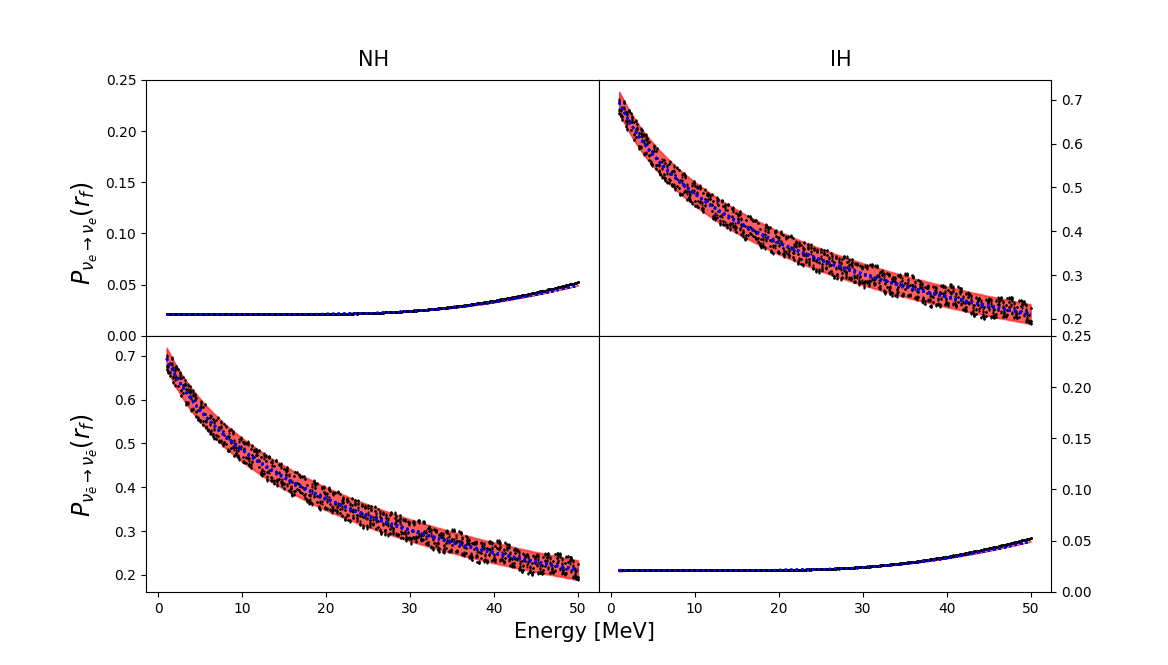
\includegraphics[width=\textwidth]{figures/theta014expNbB_t1s_energySpec_theta0_averaged.png}
    \caption[$ t=1 $ s başlangıç koşullu, theta014expNbB Modeli, 9 simülasyonun Enerjiye Karşılık Yaşama Olasılıkları.]{$ t=1 $ s başlangıç koşullu, theta014expNbB Modeli, 9 simülasyonun Enerjiye Karşılık Yaşama Olasılıkları. Her siyah nokta, sayısal sonuçların son birkaç kilometredeki ortalamasıdır. Normal hiyerarşi ile yapılan simülasyonlarda başlangıçta sadece elektron antinötrinosu bulunmaktadır. Başlangıç baryon yoğunluğu $ n_{0}=1.8\times 10^{7} $ g/cm$ ^{3} $ değerindedir.}
    \label{fig:theta014expNbB_t1s_energySpec_theta0_averaged}
\end{figure}

\begin{figure}[hbt!]
    \centering
    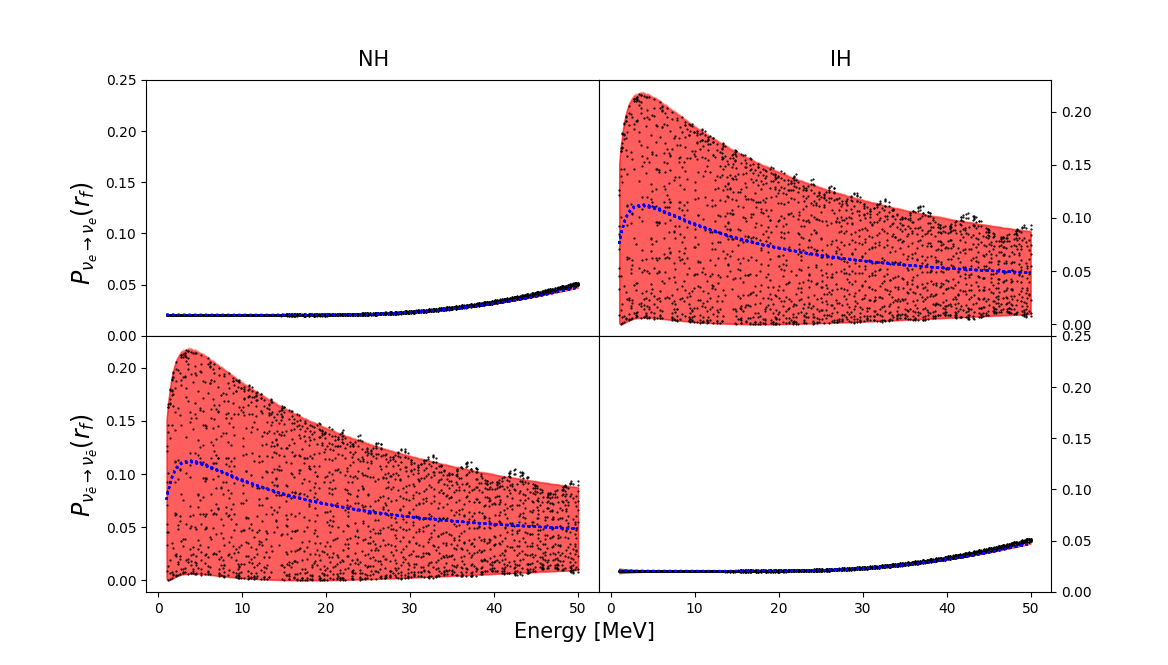
\includegraphics[width=\textwidth]{figures/theta014expNbB_t3s_energySpec_theta0_averaged.png}
    \caption[$ t=3 $ s başlangıç koşullu, theta014expNbB Modeli, 9 simülasyonun Enerjiye Karşılık Yaşama Olasılıkları.]{$ t=3 $ s başlangıç koşullu, theta014expNbB Modeli, 9 simülasyonun Enerjiye Karşılık Yaşama Olasılıkları. Her siyah nokta, sayısal sonuçların son birkaç kilometredeki ortalamasıdır. Normal hiyerarşi ile yapılan simülasyonlarda başlangıçta sadece elektron antinötrinosu bulunmaktadır. Başlangıç baryon yoğunluğu $ n_{0}=2.3\times 10^{6} $ g/cm$ ^{3} $ değerindedir.}
    \label{fig:theta014expNbB_t3s_energySpec_theta0_averaged}
\end{figure}

$ Y_{e}$ değiştiğinde MSW ve SFP rezonanslarının konumu değişir (bakınız \ref{fig:resonance_nb_Ye} numaralı şekil.) Özellikle $ Y_{e}$ değeri  $ 0.5 $ değerine yaklaştıkça rezonanslar birbirinden uzaklaşır. Bu başlangıç koşulu kurulumunda ise $ P_{SFP} $ değeri çok küçük çıkar ve SFP rezonansı adyabatik bir geçiş olur. Adyabatik geçişler de başlangıç koşullarındaki küçük değişimlerden bağımsızdır. Başka türlü ifade etmek gerekirse 9 farklı simülasyonun analitik öngörüsü aynı çıkar. Bu bölümde, kırmızı ile belirtilen hata aralığı sıfır olur ve fazların etkisi yok olur.

\section{GERÇEKÇİ MODELLER}\label{sec:gercekciModeller}
Bu bölümde, gerçekçi bir ÇÇSN modeli kullanarak simülasyonlar yapılacaktır. Yapılan simülasyonlarda nötrino elektromanyetik etkileşimin ve nötrino öz-kırılımının kollektif nötrino salınımına olan etkisi incelenecektir. Bir önceki bölümün aksine bu bölümde baryon yoğunluğu ÇÇSN modelinden alınacaktır. Özel olarak $ t=0 $ s'deki yoğunluk \cite{1987ESOC...26..325N} numaralı referanstaki SN1987A modelinden alınacak, onun üzerine \cite{Athar:1995cx} numaralı referansta tarif edilen şekilde parametrik bir şok dalgası eklenerek $ t>0 $ anlarındaki yoğunluklar elde edilecektir. Manyetik alan ise \ref{tab:simulasyonlar} numaralı tabloda verildiği gibi alınacaktır.

Baryon yoğunluğunu ve elektron kesrini veren grafik \ref{fig:t5s_nbYe2dist} numaralı şekilde verilmiştir. Tüm simülasyonlar bu profile göre yapılmıştır.

\begin{figure}[hbt!]
    \centering
    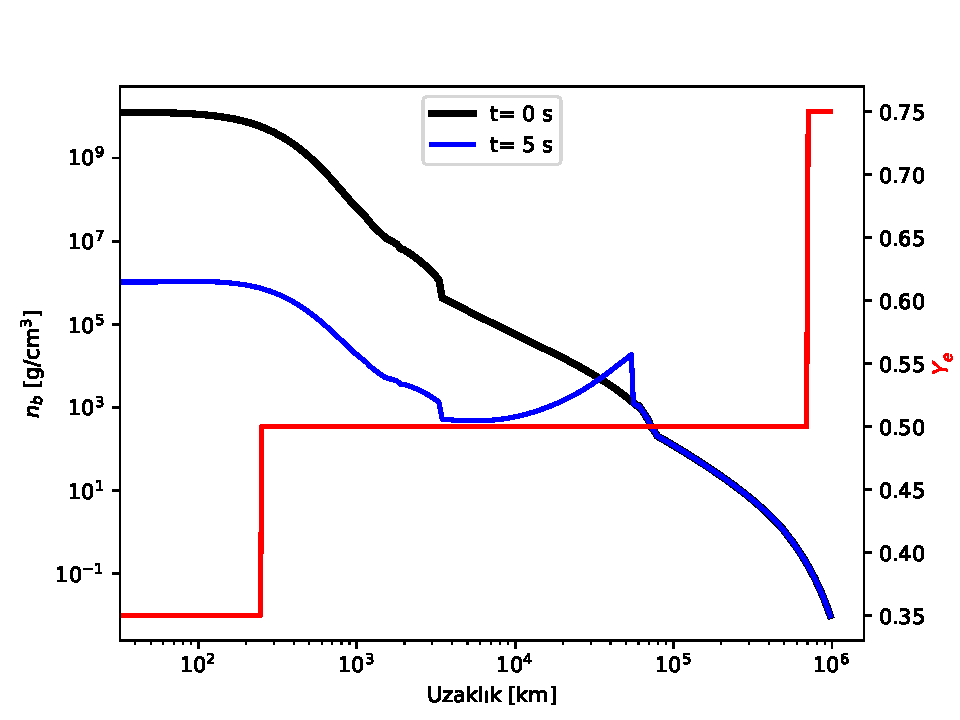
\includegraphics[width=0.9\textwidth]{figures/t5s_nbYe2dist.pdf}
    \caption[$ t=5 $s İçin Baryon Yoğunluğu ve Elektron Kesri.]{$ t=5 $s İçin Baryon Yoğunluğu ve Elektron Kesri. Yaklaşık $250$ km'de elektron kesri aniden yükselmektedir. Şok dalgasının konumu ise $55000$ km civarındadır.}
    \label{fig:t5s_nbYe2dist}
\end{figure}

ÇÇSN oluşmadan önce merkeze yakın noktalarda nötron fazlalığı bulunmaktadır \cite{Athar:1995cx}. Bu nötron fazlalığı elektron kesrini $ 0.5 $ değerinden daha küçük bir değere getirecektir. Patlama gerçekleştikten sonra açığa çıkan şok dalgası ile beraber bu nötron yoğunluğu olan bölge daha iç bölgelere taşınacaktır. Bu tezde nötron zengin bölgeyi $ 50 $ ile $ 250 $ km arasında alacağız. Bu değer bir önceki bölümdeki süreksizliğin olduğu $ r_{d} $ uzaklığına denktir. Pre-süpernova fazındayken $ r_{d} $ değeri yaklaşık $ 10^{-3} R_{\odot} $ uzaklığındadır \cite{Athar:1995cx}. Son olarak, not edilmelidir ki bu nötron zengin bölgede $ r $-işlem (r-process, rapid process) çekirdek sentezi meydana gelmektedir \cite{Janka:2006fh,Arnould:2007gh,Qian:1996xt}.

Gerçekçi simülasyonlarda ortak olan bir diğer nicelik ise nötrino parlaklığıdır. Nötrino parlaklığı, süpernova evresine yani zamana bağlı olarak düşecektir. Bu düşme aşağıdaki gibi parametrize edilir.
\begin{equation}
    L(t)= L_{0}\exp(-t/\tau)
\end{equation}
Burada $ \tau=3 $ olarak alınmıştır \cite{2017hsn..book.1605R, Mirizzi:2015eza}. $ L_{0} $ total bağlanma enerjisinden bulunabilir ve yapılan SN simülasyonuna bağlıdır. Bu çalışmada bağlanma enerjisi yaklaşık $ 10^{53} $ erg civarında seçilmiştir. Buna bağlı olarak $ L_{0}=10^{52} $ erg/s olacaktır. Bu değerler SN1987A modelini ortaya koyan çalışmalarla uyumludur \cite{fukugita2013physics}. $ t=1 $ s için $ 0.7 $ katına, $ t=5 $ s. için $0.26$ katına düşecektir. Tüm nötrino çeşnileri için aynı parlaklık değeri kullanılmıştır.

Nötrino dağılımları ise Fermi-Dirac dağılımı olarak alınacaktır. Nötrino sıcaklıkları ise $ T_{\nu_{e}}=3 $, $T_{\nu_{\bar{x}}}=4 $ ve $T_{\nu_{\bar{x}},\nu_{x}}=6 $ MeV değerleri alınmıştır. Bunun dışındaki diğer temel parametreler, son uzaklık ve nötrino istatistiksel dağılım dışında, \ref{tab:oyuncakModOrtakBasKos} numaralı tabloda verilmiştir. Ayrıca $ \delta m^{2}= 2.56 \times 10^{-15} $ MeV alınmıştır \cite{ParticleDataGroup:2018ovx}.

Aşağıdaki, \ref{fig:t5sNoCollnuNoB_distdiag10}, \ref{fig:t5sNoCollnuNoB_spectrum}, \ref{fig:t5sNoCollnuB_distdiag10}, \ref{fig:t5sNoCollnuB_spectrum} , \ref{fig:t5sCollnuNoB_distdiag10}, \ref{fig:t5sCollnuNoB_spectrum}, \ref{fig:t5sCollnuB_distdiag10} ve \ref{fig:t5sCollnuB_spectrum} numaralı grafiklerin hepsinde aynı renk kodu kullanılmıştır. Siyah renk elektron çeşnisine, mavi renk $ x $ çeşnisine, kırmızı renk anti elektron çeşnisine ve yeşil renk ise anti $ x $ çeşnisine denk gelmektedir. Spektrum grafikleri, çeşni evriminin başlangıçtaki ve simülasyonun sonundaki durumlarını gösterir. Simülasyonlar $ 70000 $ km'ye kadar yapılmıştır. Bu uzaklıktan sonra nötrinoların çeşni evrimini etkileyen bir olay olmamaktadır, yani, nötrinolar efektif olarak boşluğa ulaşmıştır diyebiliriz. Ayrıca antinötrinoların spektrumu ile nötrinoların spektrumu karışmaması için antinötrinoların spektrumu negatif enerjili gibi gösterilmiştir.

Tüm modellerde, ters hiyerarşi dikkate alındığı için MSW rezonansı antinötrino çeşnileri arasında gerçekleşecektir. 

\textbf{t5sNoCollnuNoB} adlı simülasyonda sadece nötrino madde etkileşimi dikkate alınmıştır. $ 10 $ MeV enerjileri nötrinoların uzaklığa göre çeşni evrimi \ref{fig:t5sNoCollnuNoB_distdiag10} numaralı şekilde, enerjiye göre spektrumuları ise \ref{fig:t5sNoCollnuNoB_spectrum} numaralı şekilde gösterilmektedir. $ 250 $ km uzaklığına kadar elektron kesri $ 0.35 $ değerinde olduğu için antinötrinolar bu bölgede bir adet rezonansa girmektedir. Ardından elektron kesri $ 0.5 $ değeri almıştır. Bu değeri aldığında ise antinötrinolar yaklaşık $ 30000 $ km'de tekrar MSW rezonansına girer. Son olarak $ 55000 $ km'de nötrinolar şok dalgası ile karşılaşır. Bu noktada baryon yoğunluğu yükseldiği için üçüncü MSW rezonansı meydana gelmektedir. Elektron ve $ x $ nötrinolarında ise girilen rezonansın adyabatikliğinden sapma oranında değişimler gözükmektedir. \ref{fig:t5sNoCollnuNoB_spectrum} numaralı şekilden görüldüğü üzere, meydana gelen tüm rezonanslar sadece $ 10 $ MeV için değil tüm antinötrinolara etki etmektedir. Bu durum $ t<5 $ s için geçerli değildir. Daha yüksek baryon yoğunluklarında, sadece yüksek enerjili nötrinolar üçüncü rezonansa girecektir \cite{Ekinci:2021miy}.

\textbf{t5sNoCollnuB} adlı simülasyonda nötrino madde etkileşimi ve nötrino elektromanyetik etkileşimi dikkate alınmıştır. $ 10 $ MeV enerjileri nötrinoların uzaklığa göre çeşni evrimi \ref{fig:t5sNoCollnuB_distdiag10} numaralı şekilde, enerjiye göre spektrumuları ise \ref{fig:t5sNoCollnuB_spectrum} numaralı şekilde gösterilmektedir. Başlangıçtaki yüksek manyetik alan elektron nötrinosu ve $ x $ antinötrinosunu karıştıracaktır. Çeşni bazında bakıldığında temiz bir MSW ve SFP rezonansı meydana gelmemektedir. Bir diğer taraftan $ x $ nötrinosu, etkileşimlerden etkilenmeden ayrışacaktır. \ref{fig:t5sNoCollnuB_spectrum} numaralı spektrum şekli, çeşni evrimi sonlandığında elektron nötrinosunun bir kısmının $ x $ antinötrinosuna geçtiğini gösterir. Bunun sebebi $ 250 $ km'ye kadar etkisini gösteren elektromanyetik alan etkileşimleridir. Eğer $ 250 $ km'den sonrasında elektron kesri $ 0.5 $ yerine $ 0.5 $'ten çok küçük farklı alınsaydı SFP rezonansı da meydana gelir. Nötrino öz-kırılımı dikkate alınmadığında, $ x $ antinötrinosunun ile elektron antinötrinosu aynı sıcaklığa geldiğini söyleyebiliriz. Bu "yeni" sıcaklığı veren elektron nötrinosudur. Elektron nötrinosunun sıcaklığının düşmesi ÇÇSN dinamiklerini değiştirebilir.

\textbf{t5sCollnuNoB} adlı simülasyonda nötrino madde etkileşimi ve nötrino öz-kırılımı dikkate alınmıştır. $ 10 $ MeV enerjileri nötrinoların uzaklığa göre çeşni evrimi \ref{fig:t5sCollnuNoB_distdiag10} numaralı şekilde, enerjiye göre spektrumuları ise \ref{fig:t5sCollnuNoB_spectrum} numaralı şekilde gösterilmektedir. Nötrino öz-kırılımının doğrusal olmayan etkileri \ref{fig:t5sCollnuNoB_distdiag10} numaralı şekilden gözükmektedir. Elektron ve $ x $ nötrinoları başlangıçta çok hızlı salınmaktadır. Antinötrinoların çeşni salınım genlikleri nötrinolar kadar fazla değildir ve MSW rezonansına girişleri açıkça gözükür. \ref{fig:t5sCollnuNoB_spectrum} numaralı spektrum grafiğinde ise iki adet temiz spektral yer değiştirme davranışı gözükmektedir. Spektral yer değiştirmeler nötrinolar için $ 9 $ MeV'de, antinötrinolar için $ 11 $ MeV'de gözükmektedir. Antinötrinolar MSW rezonansına da girdiği için $ 11 $ MeV'den düşük enerjili antinötrinoların spektrumları hali hazırda yer değişmiş bulunmaktadır.

\textbf{t5sCollnuB} adlı simülasyonda nötrino madde etkileşimi, nötrino öz-kırılımı ve nötrino elektromanyetik etkileşimi dikkate alınmıştır. $ 10 $ MeV enerjileri nötrinoların uzaklığa göre çeşni evrimi \ref{fig:t5sCollnuB_distdiag10} numaralı şekilde, enerjiye göre spektrumuları ise \ref{fig:t5sCollnuB_spectrum} numaralı şekilde gösterilmektedir. Bu model en gerçekçi modeldir. t5sCollnuNoB modeli ile karşılaştırıldığında manyetik momentin çeşni evrimine olan katkısı görülebilir. \ref{fig:t5sCollnuB_distdiag10} numaralı şekil ile \ref{fig:t5sCollnuNoB_spectrum} numaralı şeklin birbirinden en önemli farkı antinötrinoların spektral yer değiştirmesi kaybolmuş veya gizlenmiştir. Manyetik alan, $ x $ antinötrinoların sıcaklığını arttığından dolayı yer değiştirme kaybolmuştur. Bir diğer taraftan nötrinoların $ 9 $ MeV'de başlayan spektral yer değiştirme davranışı elektron nötrinoları için tamamlanmış ancak $ x $ antinötrinosu için tamamlanmamıştır.

\newpage
\begin{figure}[hbt!]
    \centering
    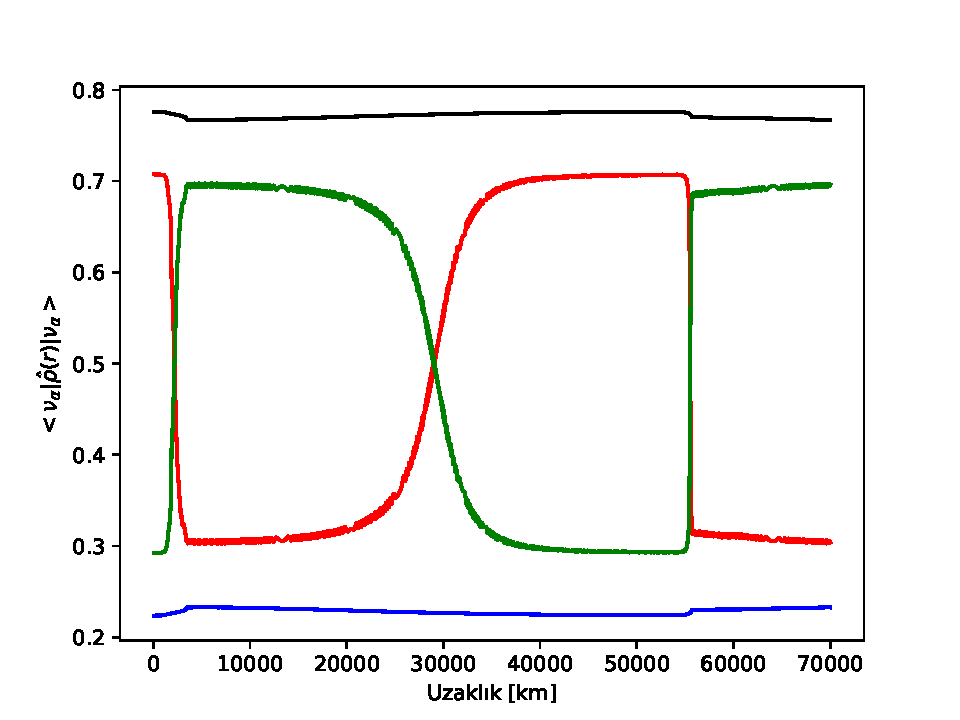
\includegraphics[width=0.9\textwidth]{figures/t5sNoCollnuNoB_distdiag10.pdf}
    \caption[t5sNoCollnuNoB Modeli, Yoğunluk Matrisinin Köşegen Elemanlarının Uzaklığa Göre Değişimi.]{t5sNoCollnuNoB Modeli, Yoğunluk Matrisinin Köşegen Elemanlarının Uzaklığa Göre Değişimi. Renk kodu: Siyah $ \nu_{e} $, mavi $ \nu_{x} $, kırmızı $ \nu_{\bar{e}} $, yeşil $ \nu_{\bar{x}} $}
    \label{fig:t5sNoCollnuNoB_distdiag10}
\end{figure}
\begin{figure}[hbt!]
    \centering
    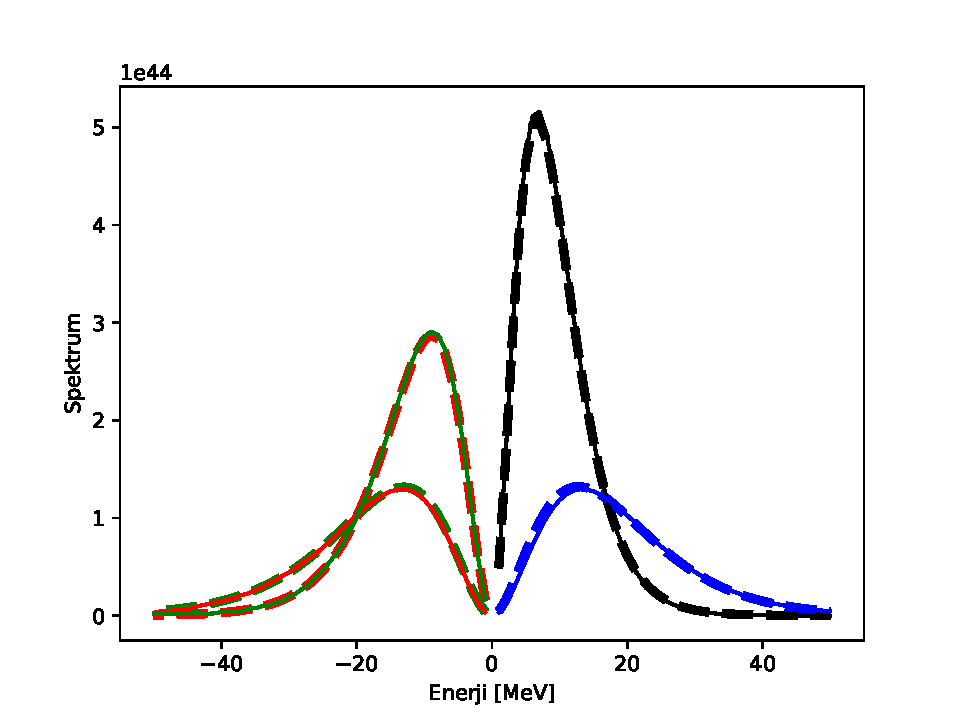
\includegraphics[width=0.9\textwidth]{figures/t5sNoCollnuNoB_spectrum.pdf}
    \caption[t5sNoCollnuNoB Modeli, Enerji Spektrumu.]{t5sNoCollnuNoB Modeli, Enerji Spektrumu. Renk kodu: Siyah $ \nu_{e} $, mavi $ \nu_{x} $, kırmızı $ \nu_{\bar{e}} $, yeşil $ \nu_{\bar{x}} $}
    \label{fig:t5sNoCollnuNoB_spectrum}
\end{figure}

\newpage
\begin{figure}[hbt!]
    \centering
    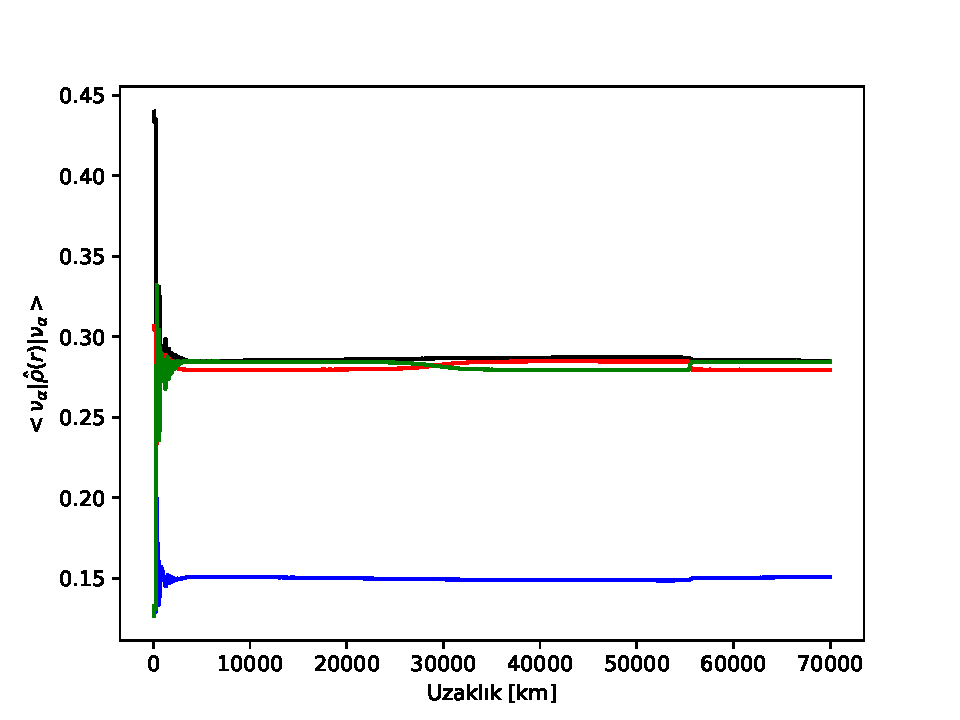
\includegraphics[width=0.9\textwidth]{figures/t5sNoCollnuB_distdiag10.pdf}
    \caption[t5sNoCollnuB Modeli, Yoğunluk Matrisinin Köşegen Elemanlarının Uzaklığa Göre Değişimi.]{t5sNoCollnuB Modeli, Yoğunluk Matrisinin Köşegen Elemanlarının Uzaklığa Göre Değişimi. Renk kodu: Siyah $ \nu_{e} $, mavi $ \nu_{x} $, kırmızı $ \nu_{\bar{e}} $, yeşil $ \nu_{\bar{x}} $}
    \label{fig:t5sNoCollnuB_distdiag10}
\end{figure}
\begin{figure}[hbt!]
    \centering
    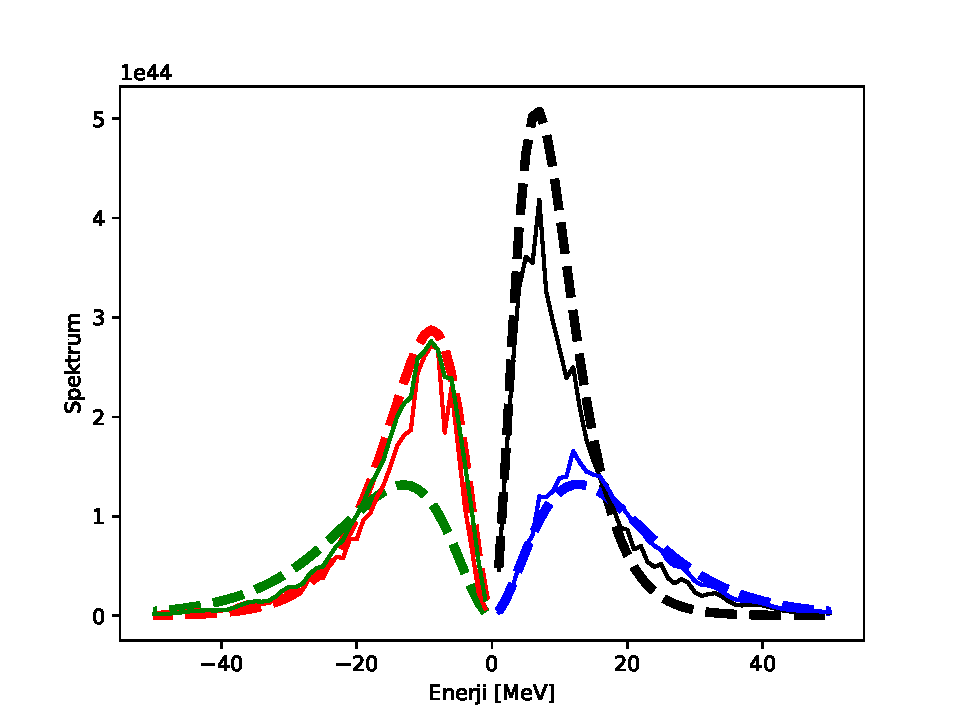
\includegraphics[width=0.9\textwidth]{figures/t5sNoCollnuB_spectrum.pdf}
    \caption[t5sNoCollnuB Modeli, Enerji Spektrumu.]{t5sNoCollnuB Modeli, Enerji Spektrumu. Renk kodu: Siyah $ \nu_{e} $, mavi $ \nu_{x} $, kırmızı $ \nu_{\bar{e}} $, yeşil $ \nu_{\bar{x}} $}
    \label{fig:t5sNoCollnuB_spectrum}
\end{figure}

\newpage
\begin{figure}[hbt!]
    \centering
    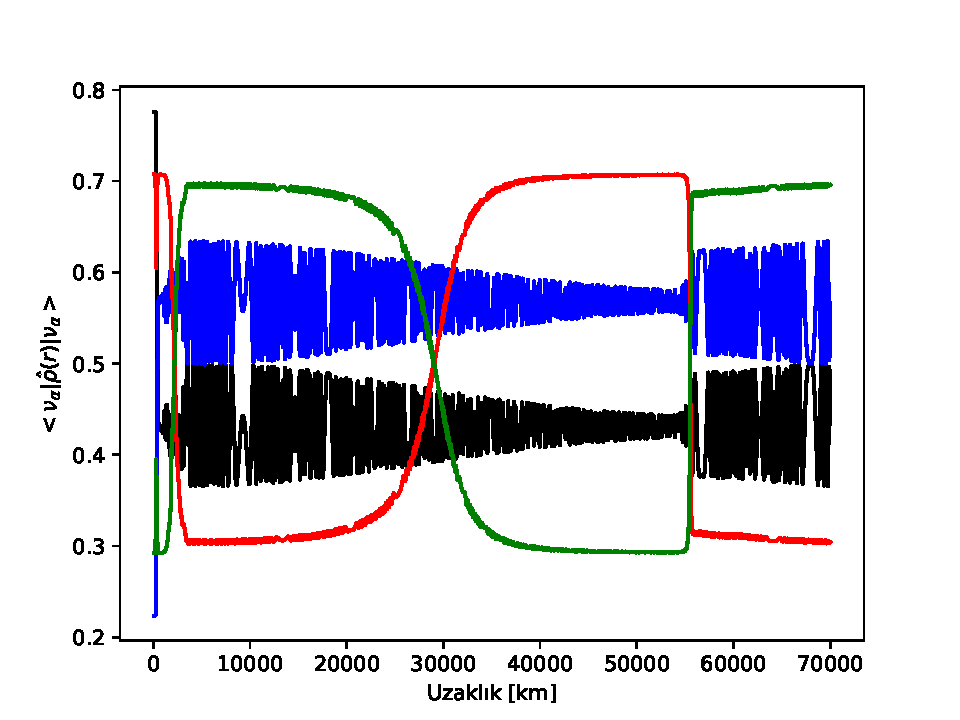
\includegraphics[width=0.9\textwidth]{figures/t5sCollnuNoB_distdiag10.pdf}
    \caption[t5sCollnuNoB Modeli, Yoğunluk Matrisinin Köşegen Elemanlarının Uzaklığa Göre Değişimi.]{t5sCollnuNoB Modeli, Yoğunluk Matrisinin Köşegen Elemanlarının Uzaklığa Göre Değişimi. Renk kodu: Siyah $ \nu_{e} $, mavi $ \nu_{x} $, kırmızı $ \nu_{\bar{e}} $, yeşil $ \nu_{\bar{x}} $}
    \label{fig:t5sCollnuNoB_distdiag10}
\end{figure}
\begin{figure}[hbt!]
    \centering
    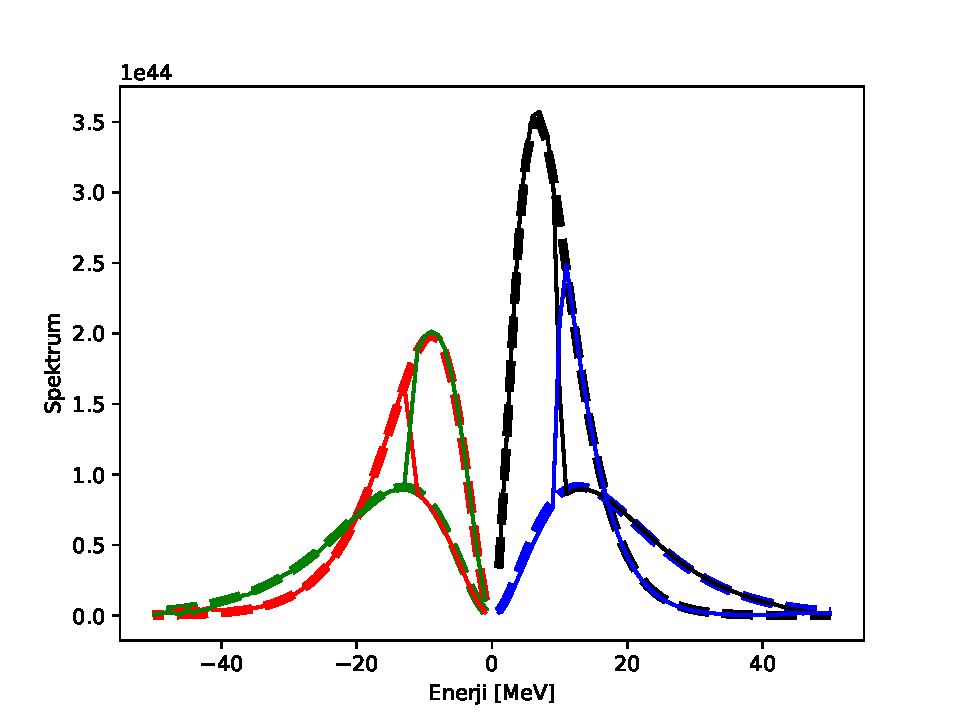
\includegraphics[width=0.9\textwidth]{figures/t5sCollnuNoB_spectrum.pdf}
    \caption[t5sCollnuNoB Modeli, Enerji Spektrumu.]{t5sCollnuNoB Modeli, Enerji Spektrumu. Renk kodu: Siyah $ \nu_{e} $, mavi $ \nu_{x} $, kırmızı $ \nu_{\bar{e}} $, yeşil $ \nu_{\bar{x}} $}
    \label{fig:t5sCollnuNoB_spectrum}
\end{figure}

\newpage
\begin{figure}[hbt!]
    \centering
    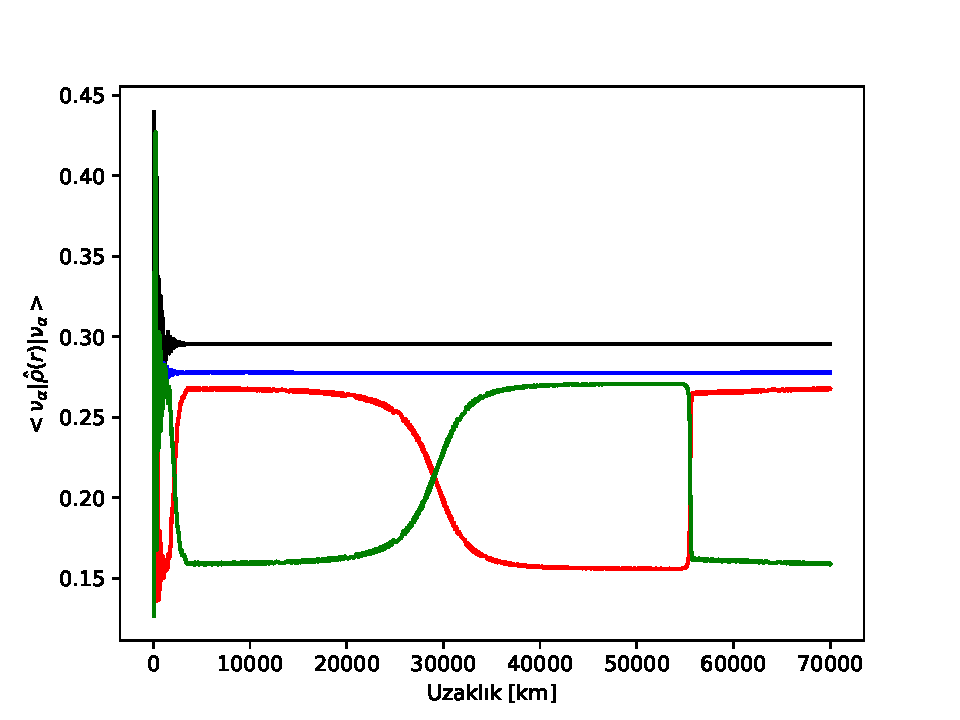
\includegraphics[width=0.9\textwidth]{figures/t5sCollnuB_distdiag10.pdf}
    \caption[t5sCollnuB Modeli, Yoğunluk Matrisinin Köşegen Elemanlarının Uzaklığa Göre Değişimi.]{t5sCollnuB Modeli, Yoğunluk Matrisinin Köşegen Elemanlarının Uzaklığa Göre Değişimi. Renk kodu: Siyah $ \nu_{e} $, mavi $ \nu_{x} $, kırmızı $ \nu_{\bar{e}} $, yeşil $ \nu_{\bar{x}} $}
    \label{fig:t5sCollnuB_distdiag10}
\end{figure}
\begin{figure}[hbt!]
    \centering
    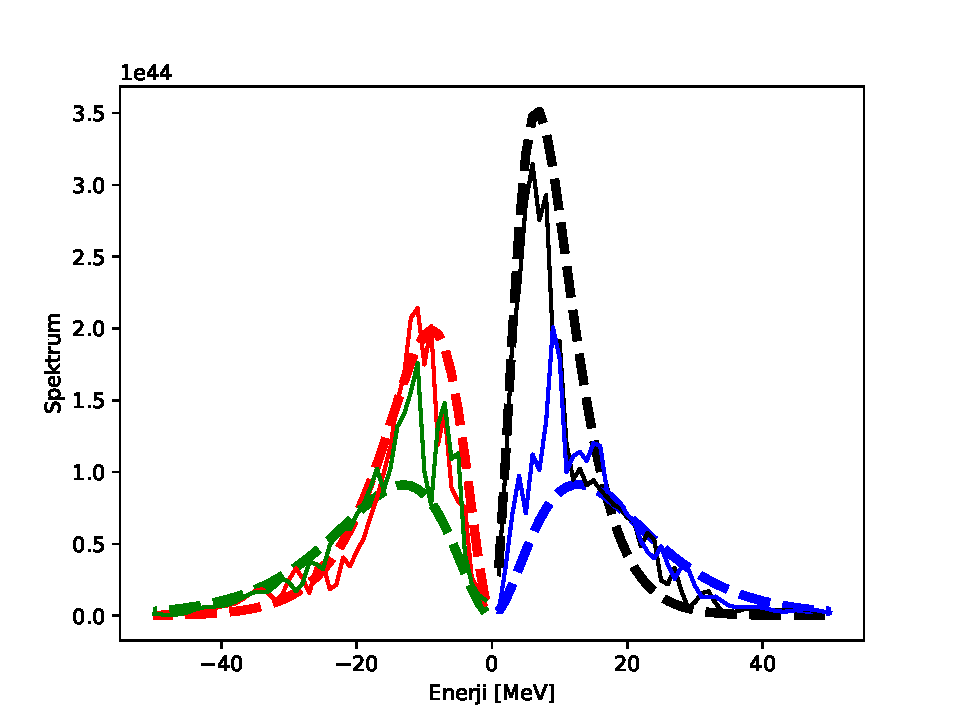
\includegraphics[width=0.9\textwidth]{figures/t5sCollnuB_spectrum.pdf}
    \caption[t5sCollnuB Modeli, Enerji Spektrumu.]{t5sCollnuB Modeli, Enerji Spektrumu. Renk kodu: Siyah $ \nu_{e} $, mavi $ \nu_{x} $, kırmızı $ \nu_{\bar{e}} $, yeşil $ \nu_{\bar{x}} $}
    \label{fig:t5sCollnuB_spectrum}
\end{figure}
\newpage
\chapter{ÇEKİRDEK SENTEZLENMESİ}\label{ch:cekirdekSentez}
\paragraph{}
ÇÇSN evrende meydana gelen en uç olaylar arasındadır. $ 8$-$9 $ Güneş kütlesinden daha büyük kütleye sahip yıldızlar olağanüstü bir patlama ile ömürlerini sonlandırırlar. Çöken materyalden açığa çıkan kütle çekim bağlanma enerjisi büyük oranda nötrinolar tarafından dışarı aktarılır \cite{1966ApJ...143..626C, 1986ARA&A..24..205W, 1989ARA&A..27..629A}. Enerji emisyonu sırasında dışarı aktarılan enerji yıldız içerisindeki elementleri uzay boşluğuna fırlatır. Bu elementler, yalnızca yıldızın ömrü boyunca hidrostatik yanmadan çıkan ürünlerini değil, aynı zamanda patlama sırasında sentezlenmiş nükleer çekirdeklerdir. Ayrıca, patlama enerjisinin $ \% 99 $'unu taşıyan nötrinolar bazı anahtar elementlerin üretilmesinde de önemli rol oynar. Açığa çıkan nötrinolar ÇÇSN başlamadan önce yıldızın çekirdeğinde termal dengeye gelmiştir. Bundan dolayı nötrinoların sıcaklığından bahsedilebilir. Nötrino sıcaklıkları \ref{tbl:AvaregedProducitionFactors} numaralı şekilde de görüldüğü üzere çeşitlilik gösterebilir. Bu sıcaklıklık farkları da nötrino etkileşimleri ile oluşmuş elementlerin üretiminde önemli rol oynar. Bu tipte etkileşimlere \emph{nu-işlemi} (nu-process) adı verilir.
\begin{table}[hbt!]
    \centering
    \begin{tabular}{|l|l|l|}
    \hline
    Çekirdek    & Düşük Enerji & Yüksek Enerji \\ \hline
    $^{7}$Li    & $ 0.04 $     & $ 0.58 $ \\ \hline
    $^{11}$B    & $ 0.31 $     & $ 1.57 $ \\ \hline
    $^{15}$N    & $ 0.09 $     & $ 0.16 $\\ \hline
    $^{19}$F    & $0.18$       & $ 0.29 $\\ \hline
    $^{138}$La  & $0.46$       & $0.77  $ \\ \hline
    $^{180}$Ta  & $0.49$       & $0.84$ \\ \hline
    \end{tabular} 
    \caption[Solar Bolluğa Göre Ortalama Üretim Faktörleri.]{Solar bolluğa göre ortalama üretim faktörleri \cite{Sieverding:2018rdt}. $ ^{16} $O üretimine göre normalize edilmiştir. Buradaki düşük veya yüksek enerji, sıcaklıklar manasındadır; Düşük enerji için $ T_{\nu_{e}}=2.8 $ MeV, $ T_{\overline{\nu}_{e}}= T_{\nu_{\mu,\tau}}=4.0 $ MeV ve Yüksek enerji için $ T_{\nu_{e}}=4.0 $ MeV, $ T_{\overline{\nu}_{e}}=5.0$ MeV, $ T_{\nu_{\mu,\tau}}=6.0 $ MeV. Burada müon ve tau nötrinoları ve antinötrinoları aynı sıcaklıktadır.}\label{tbl:AvaregedProducitionFactors}
\end{table}

Yıldız evrimi sırasında demir elementine kadar sentezlenen elementlerin, örneğin karbon, oksijen, demir gibi, bolluğunu nükleer tepkimeler yardımı ile açıklayabiliriz \cite{Burbidge:1957vc}. Öte yandan, güneş sisteminde bulunan nadir izotopların sentezlenmesi hala açık bir sorudur. Süpernova sırasında meydana gelen çekirdek sentezi Güneş sistemindeki elementlerin bir kısmının bolluğunu açıklamak için kullanılır. Ancak ÇÇSN'deki nükleer sentezleme hakkındaki bilgimiz patlama modelleri ile sınırlıdır. Çoğunlukla yapay parametreler kullanılarak yapılan patlama modelleri Güneş sistemindeki element bolluğunu tamamen karakterize edemez. Süpernova çekirdek sentezi üzerine çeşitli çalışmalarla yapılmış olsa da, \cite{1954ApJS....1..121H, 1995ApJS..101..181W, 1996ApJ...460..408T}, gözlemlenen süpernova kalıntıları ve evrimleri hala model bağımlıdır veya serbest parametre bağımlıdır. Yıldız evriminde çekirdek sentezi, tek başına demirden daha ağır elementler üretmek için yeterli olmasa da $ ^{7} $Li ve $ ^{11} $B izotopları gibi bazı izotopların üretimini sağlayarak Güneş sistemindeki bilinen elementlerin bolluğuna katkıda bulunur \cite {Sieverding:2018rdt}.

Günümüzde çok boyutlu ÇÇSN simülasyonları, son hesaplama teknolojisindeki gelişmelerle beraber daha ayrıntılı olarak gerçekleştirilebilir \cite{Janka:2017vcp}. Ancak patlama simülasyonlarının çoğu sadece birkaç yüz milisaniye kadar çalışabilir. Geç zaman ÇÇSN soğuma fazında (cooling phase) çekirdek sentezlenme hesapları için yeterli değildir. Biz bu zorlukların üstesinden gelmek için başarılı bir şekilde patlayan PUSHing yöntemi \cite{2015ApJ...806..275P} adlı, tamamen kendisi tutarlı tek boyutlu süpernova modelini kullandık. Bu model ata yıldızı (progenitor) oluşturan elementlerin her bir zaman aralığında dinamik değişimini açıklar ve neredeyse beş saniye boyunca dinamik çekirdek sentezleme hesabının yapılmasına olanak verir.

\section{PUSHing ÇÇSN MODELİ}\label{sec:PUSHing}
\paragraph{}
PUSH (Parametrized Spherically Symmetric Explosion Method) veya PUSHing modeli patlama için yapay olarak tetiklenen tek boyutlu bir ÇÇSN modelidir. Bu modelin ayrıntılı açıklamaları \cite{2015ApJ...806..275P,2019ApJ...870....1E} numaralı kaynaklarında ve PUSH yöntemini kullanarak çekirdek sentezi analizi yapan \cite{Curtis:2018vkh} numaralı kaynakta bulunmaktadır. Bu bölümde kısaca modeli açıklayıp bizim kullandığımız parametreleri vereceğiz. Bu çalışmada tek boyutlu simülasyondan elde edilen başlangıç koşullarını dikkate alınacaktır. İki boyutlu ÇÇSN için \cite{2018JPhCS.940a2054S} numaralı kaynağa başvurabilirsiniz.

PUSH simülasyonu, küresel simetrik başlangıç koşulları ile başlayıp göreli hidrodinamik denklemleri çözen AGILE \cite{Liebendoerfer:2000fw} kodunu kullanmaktadır. Kod nötrino güdümlü (neutrino-driven) mekanizmaya dayanır. Tek boyutlu simülasyonlar herhangi bir türbülans, konveksiyon veya SASI (Standing Accretion Shock Instabilities) oluşturmasa da ÇÇSN'nin temellerini anlamak için uygundur. Üstelik çok boyutlu yöntemlerin bir saniyeden öteye gidemeyecek kadar bilgisayar hesaplama maliyeti vardır. Bilgisayar kaynaklarındaki  hesaplama kısıtlaması tam çekirdek sentezleme sonuçlarını elde etmedeki çok büyük engellerden biridir. Bu nedenle, PUSH gibi parametrize edilmiş yöntemler çekirdek sentezleme hesaplaması için büyük öneme sahiptir. Çok boyutlu simülasyonlarda nötrinoların çeşnilere göre sıcaklıkları ÇÇSN'nın patlayıp patlamamasında kritik rol oynar. Başarılı bir patlama sekme (bouncing) evresinden sonra açığa çıkan şok dalgasının enerjisine bağlıdır. Açığa çıkan nötrinolar şok dalgasını hem ısıtır hem de iter. PUSH metodu şokun kinetik enerjisini besleyen nötrinoların oranını yapay olarak arttırarak şoku besler. Yani nötrinoların sıcaklıklarını arttıran serbest bir parametre kullanır. Bu ısıtmayı betimleyen yerel bir büyüklük tanımlayabiliriz.
\begin{equation}
    Q^{+}_{push}(r,t)=4\mathcal{G}(t) \int_{0}^{\infty}q^{+}_{push}(r,E)dE \text{ .}
\end{equation}
Burada 
\begin{equation} \label{eqn:PUSHartificial}
    q^{+}_{push}(r,E) \equiv \sigma_{0}\frac{1}{m_{b}}\qty(\frac{E}{m_{e}c^{2}})^{2} \frac{1}{4\pi r^{2}} \frac{d L_{\nu_{x}}}{dE} \mathcal{F}(r,E)
\end{equation}
şeklinde tanımlanmıştır. $ \sigma_{0} $, nötrinoların tipik tesir kesiti, $ m_{e,b} $ elektron ve baryon kütlesi, $ (dL_{\nu_{x}}/dE)/(4\pi r^{2}) $ terimi spektral enerji akısı $ \mathcal{G} $ ve $ \mathcal{F} $ terimleri ise PUSH simülasyonundan elde edilen uygun evrim fonksiyonlarıdır. Daha ayrıntılı hesap için \cite{2015ApJ...806..275P} numaralı kaynağı bakınız. 

Müon ve tau nötrinolarının ve antinötrinolarının sıcaklıklarını yapay olarak arttırmak kendisiyle tutarlı (self-consistent) süpernova patlaması meydana getirmektedir. Buradaki simülasyonu tetikleyen tüm parametreler, Süpernova \textit{SN1987A} 'dan esinlenmiştir. Sonuç olarak $ 18.8 $ Güneş kütlesine sahip bir ata yıldız kullanarak yaptığımız simülasyonun başlangıç parametreleri numaralı tabloda verilmiştir.
\begin{table}[hbt!]
    \centering
    \begin{tabular}{|l|l|}
    \hline
    \textbf{Parametreler} & \textbf{Değerler} \\ \hline
    Ata Yıldızın Kütlesi & 18.8 M$_{\odot}$ \\ \hline
    Kütle Kesimi (Mass Cut) & 1.5466 \\ \hline
    İzleyici (Tracer) Çıktı Sayısı & 3146 \\ \hline
    Kütle Hassasiyeti & 10$ ^{-3} $M$_{\odot}$\\ \hline
    Patlama Zamanı & $ \sim $ 4 s \\ \hline
    Patlama Enerjisi & 1.2$\times  $10$ ^{51} $ erg \\ \hline
    \end{tabular} 
    \caption[PUSH Modelinin Parametreleri.]{PUSH Modelinin Parametreleri.} 
    \label{table:ProgenitorParameters}
\end{table}

Bizim kullandığımız ata yıldız modelinde dış katmanların verisi bulunmamaktadır. \ref{fig:progenitorAbund_Temp} numaralı şekilden de görüleceği üzere, yıldızın en büyük katmanı olan Helyum (HE) katmanı çok küçük gözükmektedir. Bu şekilde almamızın sebebi simülasyonun $ t=4 $ s'de sonlaması ve şok dalgasının yaklaşık O/C katmanına gelmesidir. Yani bu katmandan sonrasında çekirdek sentezlenmesinin başlamamasıdır. \ref{fig:progenitorAbund_Temp} numaralı şekilde, tepe sıcaklığının $ t=5 $ s'deki dağılımı ve ata yıldızın (simülasyon başlamadan önceki hali) katmanları içerisindeki bazı elementlerin kütle oranlarını gösterilmektedir. Tepe sıcaklık grafiğinde, O/C katmanındaki ani değişimin sebebi şok dalgasıdır. Yani şok dalgası $ t=5 $ s süre geçtiğinde yaklaşık $3.8$ - $4.2$ Lagranjiyen kütle koordinatlarında bulunmaktadır. Grafikte arka planda bulunan renkler süpernova içerisindeki katmanları göstermektedir; Mavi Si katmanını, sarı O/Ne katmanını, mor O/C katmanını ve yeşil ise He katmanını gösterir. 

\begin{figure}[hbt!]
	\centering
	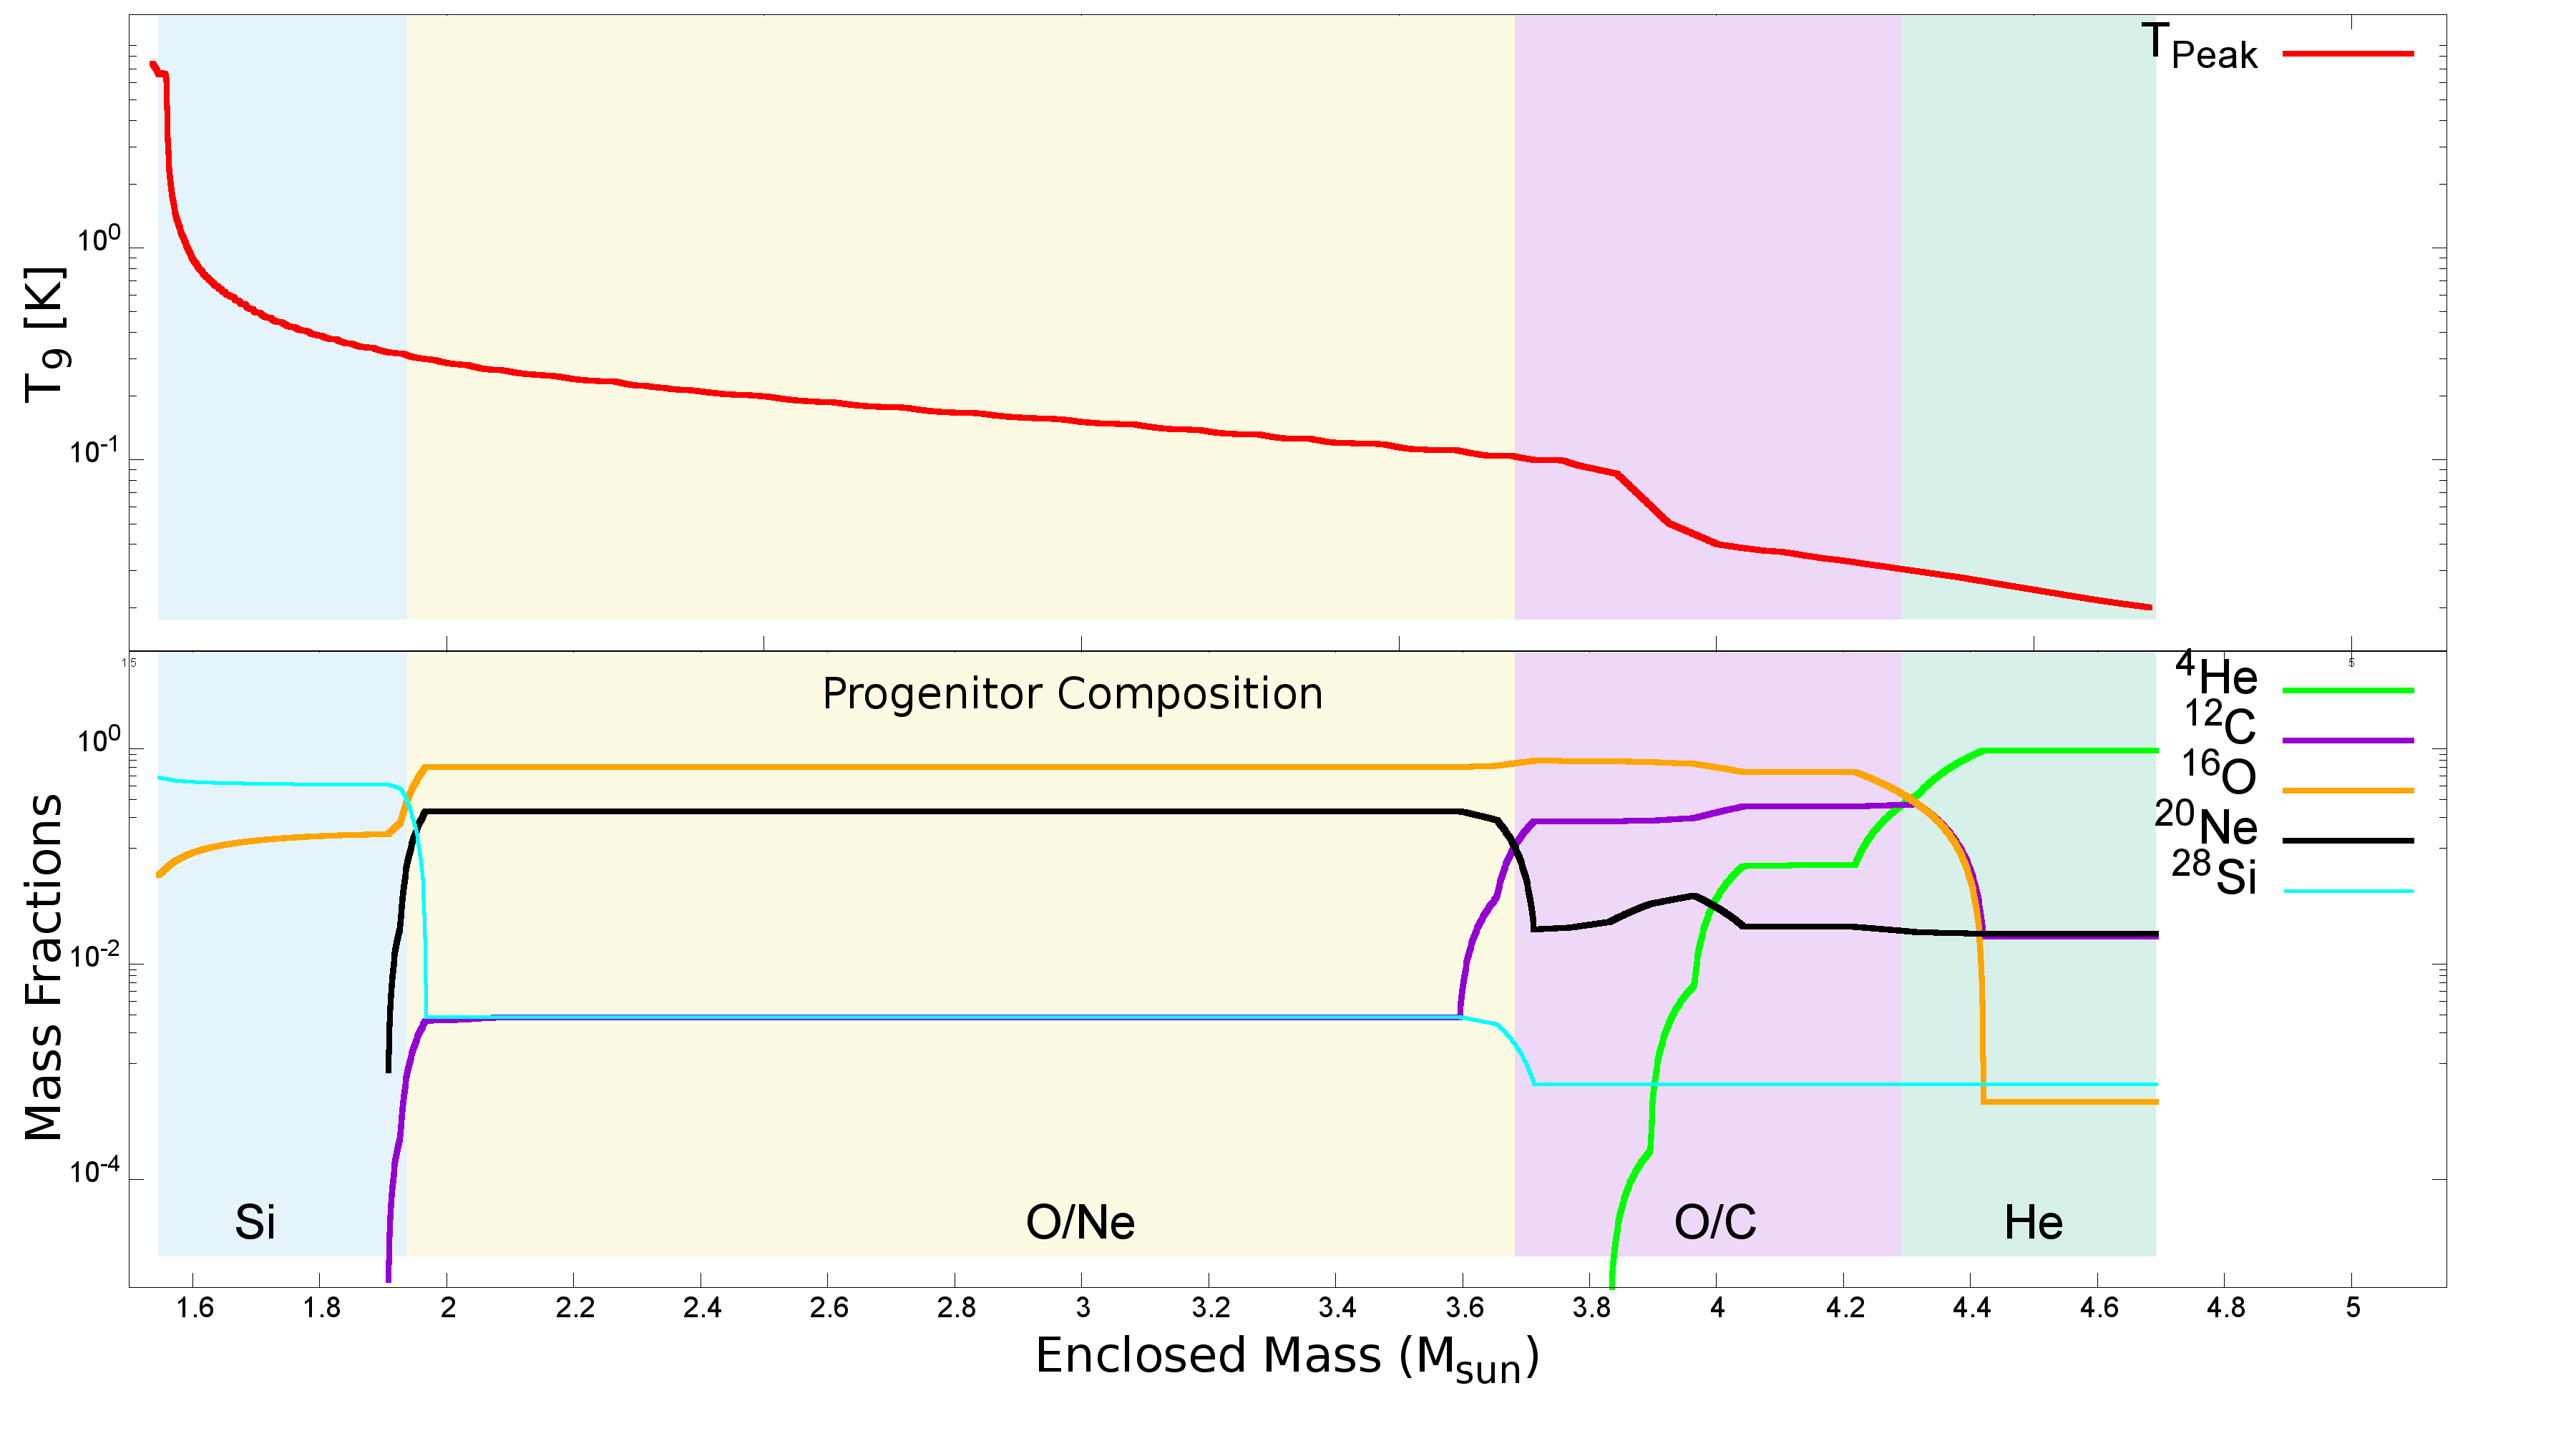
\includegraphics[width=\textwidth]{figures/progenitorAbund_Temp.png}
	\caption[Ata Yıldızın Bolluğu Ve Tepe (Peak) Sıcaklığı.]{Ata yıldızın bolluğu ve tepe (peak) sıcaklığı. Çekirdek sentez ağ simülasyonu, $ 6.5 $ GK sıcaklığında nükleer istatistiksel dengededir (nuclear statistical equilibrium.) Bu da yaklaşık Si katmanının ortasına denk gelir.}
	\label{fig:progenitorAbund_Temp}
\end{figure}

Tepe sıcaklığının nükleer istatistiksel dengeyi nasıl etkilediğini ve çekirdek sentezlenme hakkındaki detayları göreceğiz. Bunun için termonükleer reaksiyon ağı (thermonuclear reaction network) oluşturmamız gerekecektir.

\section{TERMONÜKLEER REAKSİYON AĞI}\label{sec:termoNukleerReakAg}
\paragraph{}
Termodinamik değişkenleri belirlemek için sadece çekirdek bolluğuna ek olarak büyük ölçekli termonükleer reaksiyon ağına ihtiyaç duyulur. Bu bölümde, çiftlenmiş adi diferansiyel denklemler kümesi olan termonükleer reaksiyon ağı evrimlerini inceleyeceğiz.

Başlangıç noktası olarak en genel reaksiyonu yazalım.
\begin{equation}
    \dots a+B \rightarrow C+d+ \dots \text{ .}
\end{equation}

Reaksiyon çeşitlerini, transfer reaksiyonları ($ ^{15}N(p,\alpha)^{12}C $), yakalama (capture) reaksiyonları ($ ^{3}He(\alpha,\gamma)^{7}Be $), zayıf reaksiyonlar ($ p(p,e^{+}\nu_{e})d $) veya bozunumlar ($ ^{56}Ni\rightarrow^{56}Co+e^{+}+\nu_{e} $) olarak kategorize edebiliriz. Bunlara ek olarak üçlü $ \alpha $-işlemi gibi, üç çekirdekten oluşan reaksiyonlar da önemlidir. Reaksiyon sonucunda her bir tepkiyen (reactant) sayı yoğunluğu, $ n_{i} $, zamanla ve reaksiyon hızı, $ r $, ile değişecektir.
\begin{equation}\label{eqn:networkDif1}
    \frac{d n_{i}}{d t}=\sum_{j} \mathcal{N}^{i}_{j}r_{j}+\sum_{j,k} \mathcal{N}^{i}_{j,k}r_{j,k}+\sum_{j,k,l} \mathcal{N}^{i}_{j,k,l}r_{j,k,l} \text{ .}
\end{equation}

Enerji-momentumun ve toplam elektrik yükün ağ hesaplaması sırasında korunması gerekmektedir. Burada  $ \mathcal{N} $ pozitif olursa oluşum (creation) negatif olursa yıkım (destruction) tepkimesi olur. $ \mathcal{N} $ ifadesinin tanımı 
\begin{equation}
    \mathcal{N}^{i}_{i}=N_{i},\quad \mathcal{N}^{i}_{j,k}=\pm \frac{N_{i}}{\abs{N_{j} }!\abs{N_{k} }!}\quad \dots
\end{equation}
şeklinde olur. Bu ifadede pay kısmı ayırt edilemez (indistinguishable) parçacık sayımından gelmektedir.

Sayı yoğunluğunu her bir çekirdeğin bolluğuna dönüştürmek için yeni değişkenler tanımlamamız gerekir. Her şeyden önce, her bir çekirdeğin nükleer bolluğu veya molar kesri $ \mathbf{Y}_{i}=\frac{n_{i}}{\rho N_{a}} $ şeklinde tanımlanır. Burada $ \rho $ yoğunluk, $ N_{a} $ ise Avagadro sayısıdır. Her reaksiyon tipi için reaksiyon hızı $ r $ değişecektir. Örneğin yavru çekirdeklerin (daughter nuclei) bozunmasında veya kütlesiz parçacıklar ile reaksiyona girmesinde reaksiyon hızı $ r_{i}=\lambda Y_{i} $ şeklinde yazılır ki $ \lambda $ bahsedilen reaksiyonun bozunma hızıdır. Eğer \eqref{eqn:networkDif1} numaralı denklemi tekrar yazarsak,
\begin{equation}\label{eqn:networkDif2}
    \frac{d Y_{i}}{dt}=\sum_{j}  \mathcal{N}^{i}_{j} \lambda_{j}Y_{j}+ \sum_{j,k} \mathcal{N}^{i}_{j,k} \qty(\frac{\rho}{m_{a}}) \expval{j,k}Y_{j}Y_{k}+ \sum_{j,k,l} \mathcal{N}^{i}_{j,k,l}\qty(\frac{\rho}{m_{a}})^{2} \expval{j,k,l}Y_{j}Y_{k}Y_{l} \text{ ,} 
\end{equation}
ifadesini elde ederiz. Burada $ \expval{i,j} $ yıldızsal (stellar) reaksiyon hızıdır. Bozunma hızı $ \lambda $ ise bozunan parçacığın bozunma hızı ile orantılıdır. Bu değerler hem sayısal simülasyonlarla hem de deneylerle elde edilir. Üç cisim etkileşimleri (three-body interactions) nadiren meydana gelmesine rağmen dikkate alındığında sonuçlarda dramatik etkiye sebep olacaktır. Yukarıda bahsedilen kütle kesri ise $ X_{i}=A_{i}Yi=\frac{\rho_{i}}{\rho} $ şeklinde tanımlanmıştır. Denklemlerdeki baryon korunumunu sağlamak için $ \sum_{i}Y_{i}A_{i}=1 $ ifadesi her an sağlanmalıdır.

Ağı betimleyen \eqref{eqn:networkDif2} numaralı denklem takımını çözebilmek için başlangıç yoğunluğunu ortamın sıcaklığı bilinmelidir. Ayrıca, başlangıçtaki madde bileşimi ve elektron kesri $ Y_{e} $, yani ata yıldızın içeriği hakkında da bilgi sahibi olunması gerekecektir. Eğer sıcaklık ve yoğunluk yeteri kadar yüksek ise nükleer reaksiyonlar iki taraflı olacaktır. Yani yıkım ve oluşum reaksiyon hızları eşit olacaktır ($ \beta $ bozunumu hariç.) Bu durumda ortamdaki madde \emph{nükleer istatistiksel dengeye} (NİD) ulaşmış olacaktır. NİD'de çekirdek sentezlenmesi olmaz. Çekirdek sentezleme hesaplama zamanını azaltmak için nükleer ağ kodu NİD'den çıktığı noktadan başlar. Bu çalışmada NİD sıcaklığı $ 6.5 $ GK civarıdır ve ağ simülasyon kodu $ 6.5 $ GK'den düşük noktalarda çalışacaktır. Böylece gereksiz ve çok katı salınan (stiff) diferansiyel denklem sistemi çözmemize gerek kalmayacaktır.

Nötrino-çekirdek etkileşimleri düşük tesir kesitlerinden dolayı ihmal edilmektedir. Diğer taraftan ÇÇSN'nın merkeze yakın noktalarında nötrino-çekirdek etkileşimlerinin etkileri görülebilir. Bu etkileşimler yüklü ve yüksüz etkileşimler olacaktır. \ref{sec:maddeIleEtkilesim} bölümünde kütleli nötrinolar için etkileşim potansiyelleri ve Hamiltonyenler'i verilmiştir. Tezin çekirdek sentezi bölümünde ise nötrinolar kütlesiz parçacıklar olarak alınacaktır. Nötrino salınımlar dikkate alınarak yapılan çalışmalar için \cite{Wu:2014kaa,Kusakabe:2019znq} numaralı kaynaklarına bakınız. Bu durumda nötrinolar da fotonlar gibi davranacak ancak Fermi-Dirac istatistiğine uyacaktır. Ayrıca elektromanyetik etkileşime de girmeyecekler. Nötrinoların reaksiyon hızı 
\begin{equation}
    \lambda_{\nu}=N\expval{\sigma \phi(E_{\nu},T_{\nu})}
    \end{equation}
şeklinde verilir.

\section{NÖTRİNO İŞLEMİ}\label{sec:NotrinoIslem}
\paragraph{}
Süpernova nötrinoları, proto-nötron yıldızının içinde termal ve kimyasal dengededir. Patlama sırasında nötrinosferden çıkan nötrinolar, sıcak ve yoğun yıldız ortamından geçerler. Nötrinoların tipik tesit kesiti çok küçük olsa bile, nötrino-çekirdek etkileşimi aşırı koşullarda önemli hale gelir. Aslında, yüksüz akım etkileşimi ile çekirdeği uyarabilecek veya yüklü akım etkileşimi ile proton/nötron sayısını değiştirebilecek kadar enerjiye sahiptirler. Bu etkileşimler, çekirdek sentezlenme sürecini etkiler \cite{Woosley:1989bd}. Nötrinoların yoğun madde içerisinde çekirdek sentezleme olayına kısaca \textit{nötrino işlemi} veya \emph{$ \nu $-işlemi} adı verilir. Bu bölümde nötrino işlemini kısaca tanıtacağız ve çekirdek sentezleme hesaplamalarımızın sonucunu özetleyeceğiz.

Birçok $ \nu $-işlem çekirdek sentezleme çalışmasında, nötrinolardan kaynaklanan çekirdek üretimini belirlemenin iki yolu vardır. Birincisi, nötrinolar yeni çekirdekleri doğrudan sentezleyebilir, örneğin, $ ^{12} $C($ \nu\text{ ,}\nu p $)$ ^{11} $B tepkimesi sayesinde. Karbon 12 atomları, nötrinolar tarafından yüksüz akım yoluyla uyarılır ve uyarılmış karbon, bir proton ile boron 11'e bozunur. Bu etkileşim esas olarak $ ^{11} $B elde etmekten sorumludur. İkinci olarak, nötrinolar, $ ^{7} $Li ve $ ^{26} $Al gibi bazı çekirdek bolluklarını önemli ölçüde değiştirebilen parçalanma reaksiyonunun hızını artırabilir \cite{Sieverding:2018rdt}.

$ ^{7} $Li ve $ ^{11} $B hafif elementlerinin kırılgan yapıları nedeniyle yıldız ortamında üretilmesi zordur. Bu çekirdekler, yüklü akım etkileşimleriyle kolayca yok edilir. Öte yandan, $ ^{7} $Li ve $ ^{11} $B çekirdeklerinin Güneş içerisindeki bollukları açıklamak için bir mekanizmaya ihtiyaç duyulmaktadır \cite{2003ApJ...591.1220L}. ÇÇSN içerisindeki nötrino işlemi, hafif çekirdek üretimini açıklamak için en umut verici mekanizmadır. Çekirdek sentezleme ağı hem yüksüz hem de yüklü akım etkileşimlerini içerir. Bahsedilen sentez ağı \ref{fig:li7b11Network} numaralı şekilde gözükmektedir.

\begin{figure}[hbt!]
	\centering
	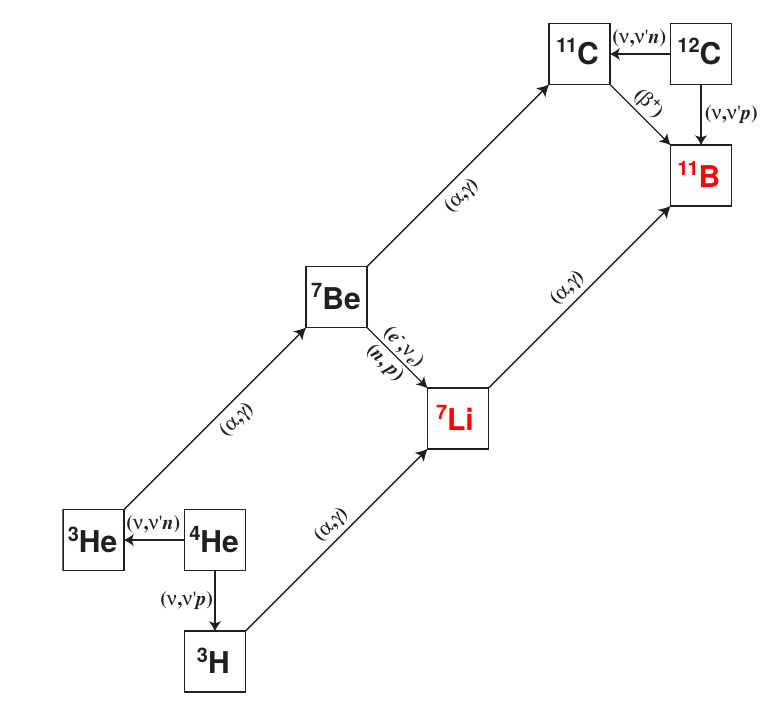
\includegraphics[width=\textwidth]{figures/li7B11_diagram}
	\caption[$ ^{7} $Li ve $ ^{11} $B Çekirdeklerinin Sentezleme Şeması.]{$ ^{7} $Li ve $ ^{11} $B çekirdeklerinin sentezleme şeması. Bu şekil \cite{Suzuki:2006qd} numaralı kaynaktan şekilden esinlenerek çizilmiştir.}
	\label{fig:li7b11Network}
\end{figure}

Nötrino işlemi çekirdek sentezlenmesinde, sadece nötrinoların akısı nihai bollukları etkilemekle kalmaz, aynı zamanda nötrino enerji spektrumu da üretim faktörlerini değiştirir. \cite{Sieverding:2018rdt} numaralı makaleye göre, yüksek enerjili nötrinolar için ortalama $ ^{7} $Li üretim faktörü, düşük enerjilerden on kat daha büyüktür (bkz. \ref{tbl:AvaregedProducitionFactors} numaralı tablo.) Bu dramatik farklılığın nedeni, yüksüz akım etkileşimlerinin büyük ölçüde nötrino enerjilerine bağlı olmasıdır. Bunun yanında $ ^{138} $La gibi çekirdekler, yüksüz akım etkileşiminden iki kat daha fazla oranda yüklü akım etkileşimleri ile üretilir. Bu nedenle, tüm $ \nu $-işlem çekirdekleri ayrı ayrı incelenmelidir.

\section{NÖTRİNO-İŞLEM SİMÜLASYON SONUÇLARI}\label{sec:NotrinoIslemSimSonuc}
\paragraph{}
Yapılan nötrino-işlem simülasyon sonuçlarını irdelemeden önce, PUSHing ÇÇSN model parametrelerinin netleştirilmesi gerekir. Çekirdek sentezi kodu tarafından kullanılan bazı termodinamik değişkenler aşağıda açıklanmıştır. Patlama sırasında nötrinoların sıcaklığı ve parlaklığı, patlamanın hangi fazda olduğuna, yani zamana göre değişir. Proto-nötron yıldızının içi, nükleer yoğunlukta olduğundan nötrinolar termal dengeye ulaşır. ÇÇSN simülasyonunun başlangıcında nötrinosferden yayılan nötrinolar görece soğuktur. Nicelik olarak değerleri \ref{fig:nuTemp} numaralı şekilde gösterilmiştir. Bir süre sonra demir çekirdek çöker ve birkaç milisaniye içinde çöken malzeme, proto-nötron çekirdeğine çarpar ve seker (bouncing.) Sekmenin hemen ardından şok dalgası oluşur. Açığa çıkan nötrinoların sıcaklığı $50$ MeV'e kadar çıkar. Buraya kadar olan olaylara \emph{patlama} (explosion) adı verilir ve patlamanın başlangıcı, sekmenin olduğu andır. Sekme fazının akabinde sıcak nötrinolar, proto-nötron yıldızının yakınındaki malzemeyi ısıtır ve onları uzaya doğru iter. Nötrinolar yardımıyla şok dalgasını ısıtmak ve iç malzemeyi dışarı itmek \emph{nötrino güdümlü mekanizma} (neutrino driven mechanism) olarak adlandırılır. Nötrinoların parlaklığı, evrendeki en uç değerlerden biri olan $10^{58} $ erg/s'ye ulaşır. Her bir nötrino tipinin parlaklıkları şekil \ref{fig:nuLum}'da gösterilmiştir.

\begin{figure}[hbt!]
    \centering
    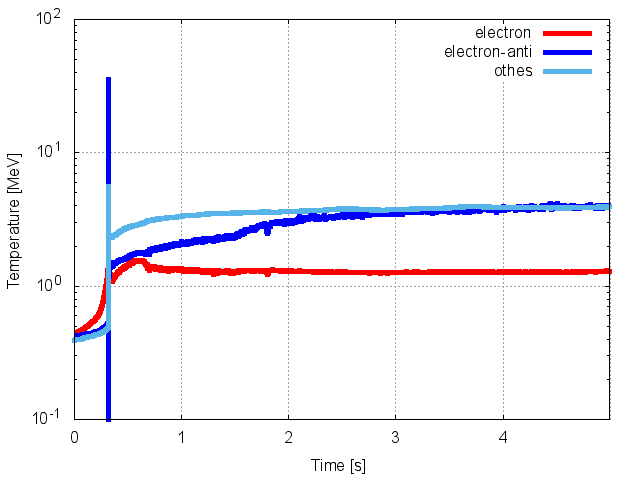
\includegraphics[width=\textwidth]{figures/nuTemperature}
    \caption[ÇÇSN Simülasyonunda Açığa Çıkan Her Nötrino Çeşnisinin Sıcaklığı]{ÇÇSN Simülasyonunda açığa çıkan her nötrino çeşnisinin sıcaklığı. Sıcaklığın $ 10^{-3} $ MeV civarına düştüğü an sekmenin olduğu andır ve bu dramatik değişim sayısal hatadan kaynaklanır. Sekme öncesinde elektron çeşnisinin sıcaklığı yüksek iken patlamadan sonra elektron çeşnisinin sıcaklığı düşük olur. Bu sıcaklık farkının en önemli sebebi nötrinoların küçük tesir kesitinin çeşniye göre küçük farklılıklar oluşturmasıdır. Elektron nötrinosunun tesir kesiti diğerlerine göre büyüktür ve proto-nötron yıldızından ısıl olarak ayrışması daha dış katmanlarda olur. Bu da elektron nötrino sıcaklığının düşük olmasına sebep olur. Daha ayrıntılı bilgi için \cite{Mathews:2014qba} numaralı kaynağın içeriğine ve bu kaynaktaki 3 numaralı şekle bakınız.}
    \label{fig:nuTemp}
\end{figure}
\begin{figure}[hbt!]
    \centering
    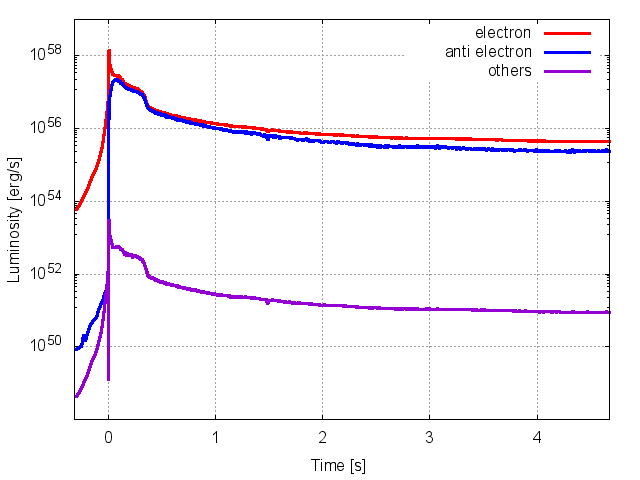
\includegraphics[width=0.7\textwidth]{figures/nuLuminosity}
    \caption[ÇÇSN Simülasyonunda Açığa Çıkan Her Nötrino Çeşnisinin Akısı.]{ÇÇSN simülasyonunda açığa çıkan her nötrino çeşnisinin. Bu şekilde, ÇÇSN'nın başlama zamanı $ 0 $ s'dir ve \eqref{fig:nuTemp} numaralı şekilde gözüken sayısal hata bu grafikte de mevcuttur.}
    \label{fig:nuLum}
\end{figure}

Sonuçlar, ortamın sıcaklığını ve yoğunluğunu, izleyicilerin mesafe değişimini, elektron fraksiyonunu, her bir nötrino çeşnisinin parlaklığını ve her bir SN izleyicisi için geçerli sıcaklıkları (zamana bağlı) içermektedir. Ayrıca $n$, $p$, $ ^{3} $He, $ ^{4} $He, $ ^{12} $C, $ ^{14} $N, $ ^{16}O, $, $^{20} $Ne, $ ^{24} $Mg, $ ^{28} $Si, $ ^{32} $S, $ ^{36} $S, $ ^{36} $Ar, $ ^{ 40} $Ca, $ ^{44} $Ti, $ ^{48} $Cr, $ ^{50} $Ti, $ ^{52} $Fe, $ ^{54} $Fe, $ ^{56} $Fe, $ ^{56} $Ni, $ ^{58} $Fe, $ ^{60} $Fe, $ ^{62} $Fe ve $ ^{62} $Ni çekirdeklerinin bollukları başlangıç koşulu olarak verilir. Bu çekirdekler, ata yıldızın kütlesine bağlı olarak yıldız evriminde üretilmiştir. Ata yıldızın içeriğindeki tüm çekirdekler dahil edilmemektedir, yani daha yüksek kütleli ata yıldız modelleri dikkate alınmadığı için, ağır izotoplar olmak üzere birçok radyoaktif izotopu hariç tutuyoruz. Bu ağır izotoplar, ağır $ \nu $-elementler üretmemizi sağlayacaktır. Temel olarak, çekirdek sentezleme kodu, her izleyicinin içerisinde bulunan her izotop için çiftlenmiş diferansiyel denklemler çözer. Çalıştırılan kodda $1988$ farklı çekirdek türü ve $3146$ izleyiciyi bulunmaktadır. Bu çekirdek türlerin bazılarının bollukları sıfırdır. Bol sıfır bulunan diferansiyel denklem sistemleri çözmek için seyrek matris (sparse matrix) tekniği kullanılır. Bu teknik sayesinde büyük miktarda bilgisayar gücünden tasarruf edilir. Çekirdek sentezleme kodunun çözümleri daha hızlı analiz etmek ve genel sentezleme eğilimine bakmak için, bu çalışmayı $ ^{7} $Li, $ ^{11} $B, $ ^{15} $N ve $ ^{19} $F gibi hafif $ \nu $-işlemi elemanlarını analiz etmekle sınırlandırdık.

SN modelinin özellikleri \ref{table:ProgenitorParameters} numaralı tabloda ve başlangıç kütle kesirleri ise \ref{fig:progenitorAbund_Temp} numaralı şekilde (alt panel) verilmiştir. Ata yıldızın bileşimi ve termodinamik değişkenler patlama için uygundur. Bunun anlamı kullandığımız ÇÇSN modeli başarıyla patlamaktadır. \cite{Sieverding:2018rdt} numaralı kaynak ve \cite{Kusakabe:2019znq} numaralı kaynaktan farklı olarak, $ ^{12} $C çekirdeğinin başlangıç bolluğu, O/Ne bölgesinin sonunda keskin bir şekilde artmaz. Bu da, o bölgedeki $ ^{7} $Li ve $ ^{11} $B üretim oranını değiştirir.
\begin{figure}[hbt!]
    \centering
    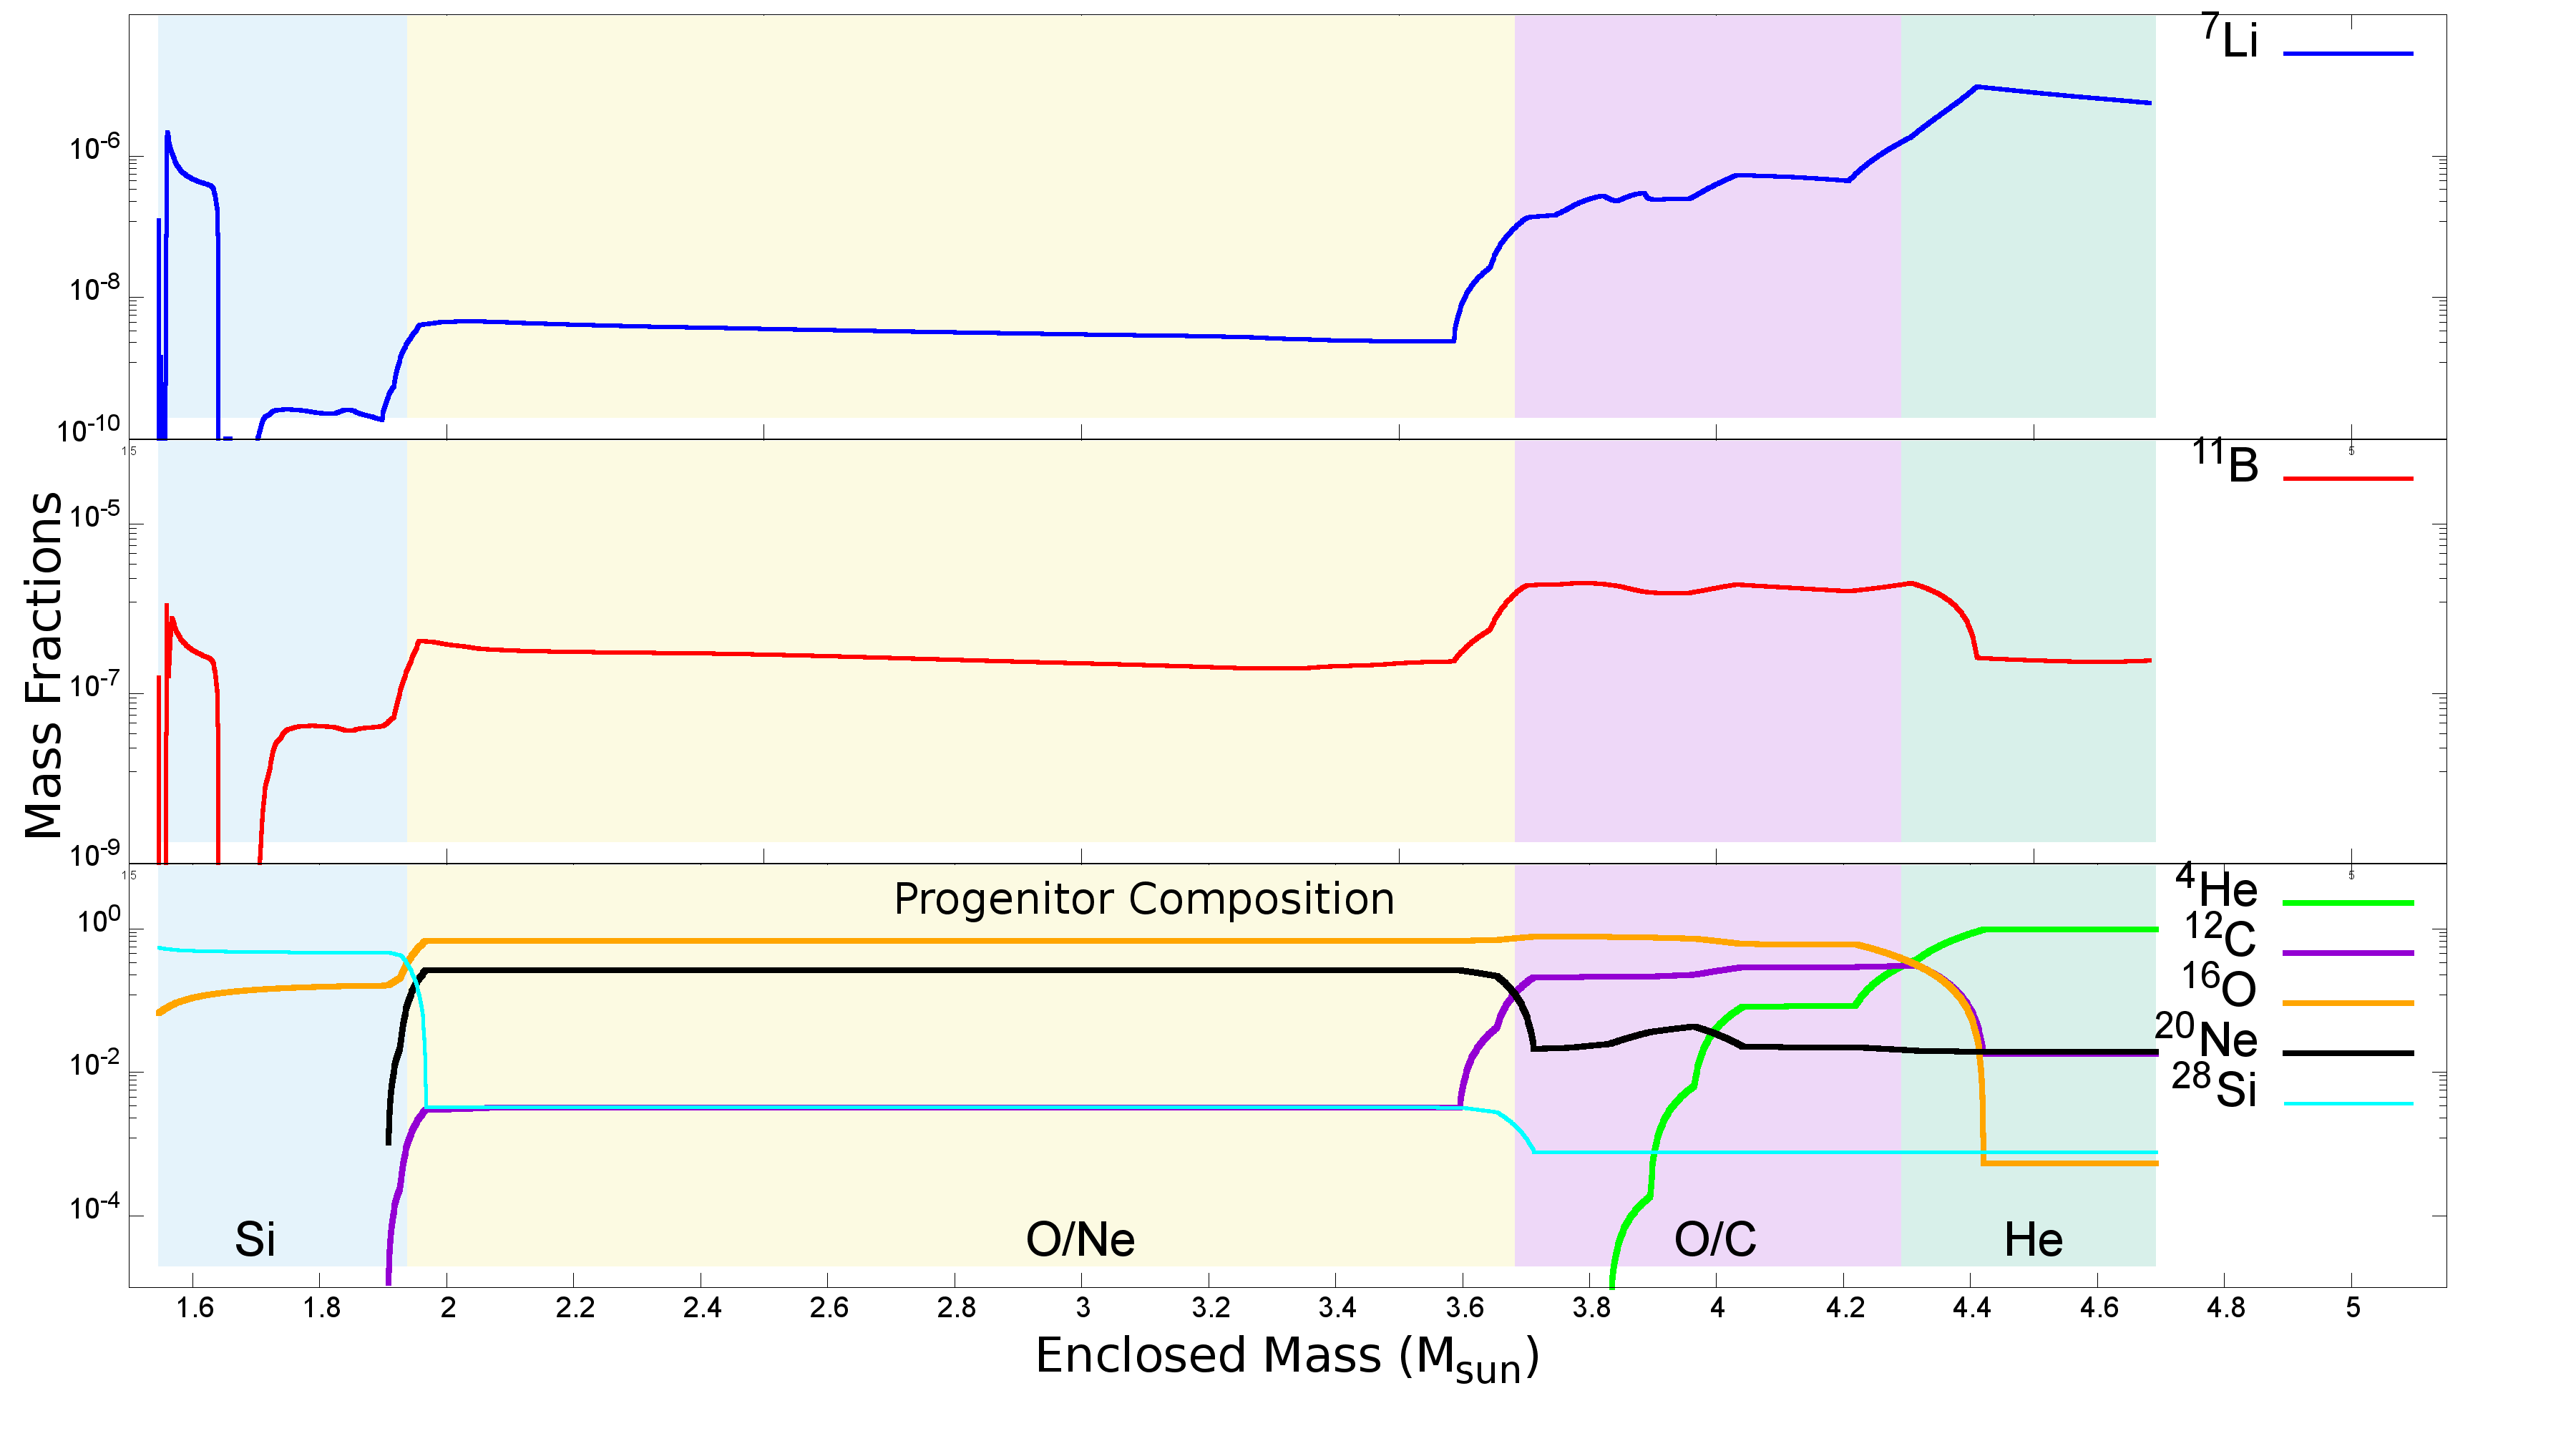
\includegraphics[width=\textwidth]{figures/abundadecay_li7b11}
    \caption[$ ^{7} $Li ve $ ^{11} $B Çekirdeklerinin Kütle Kesirleri.]{$ ^{7} $Li ve $ ^{11} $B çekirdeklerinin kütle kesirleri. Burada $ ^{7} $Li ve $ ^{11} $B üretimleri O/C katmanında arttığı görülmektedir.}\label{fig:abundadecay_li7b11}
\end{figure}

\ref{fig:abundadecay_li7b11} numaralı şekilde, $ ^{7} $Li ve $ ^{11} $B çekirdeklerinin SN katmanlarına göre karakteristik üretimi gösterilmektedir. $ ^{7} $Li bolluğunun yükselişi Si katmanında başlar ancak O/Ne katmanında sabit kalır. Çok iç bölgede (inner most region), $ ^{7} $Li ve $ ^{11} $B çekirdeklerinin ana üretim mekanizmaları, $ ^{7} $Li için $ ^{3} $He($ \alpha $,$\gamma$)$ ^{7} $Be( $ \beta^{+} $)$ ^{7} $Li ve $ ^{11} $B için $ ^{3} $H($ \alpha $,$ \gamma $)$ ^{7} $Li ($ \alpha $,$ \gamma $)$ ^{11} $B tepkimeleridir. Çok iç bölgedeki bileşiminde yeterli $ ^{4} $He çekirdeği yok gibi görünse de, ÇÇSN patlama mekanizması ile bu bölgede yüksek miktarda $ \alpha $ parçacığı asılı kalır. Bu duruma \emph{$ \alpha $-zengin dondurması} ($\alpha$-rich freeze-out) adı verilir. Ayrıca, Si katmanındaki nötrino akısı, dış katmanlardan çok daha büyüktür. Nötrinolar O/C ve He katmanlarına geldiğinde, şekil \ref{fig:li7b11Network}'deki tüm etkileşimler çok hızlı gerçekleştiği için çekirdek bollukları tekrar artacaktır. $ ^{4} $He ve $ ^{12} $C bollukları, $ ^{7} $Li ve $ ^{11} $B üretim hızını O/C ve O kabuklarında doğrudan etkiler. Bu etkinin asıl sebebi nötrinolardır. Özellikle He katmanında nötrino akıları en düşük değere sahip olsa bile bahsedilen çekirdeklerin üretim hızı artacaktır. \ref{fig:abundadecay_li7b11} numaralı şekil hakkında son bir not vermek gerekirse, elektron nötrino akısını azaltabilen nötrino salınımları, bu çalışmada dikkate alınmamıştır. 

\begin{figure}[hbt!]
	\centering
	\begin{subfigure}{.49\textwidth}
		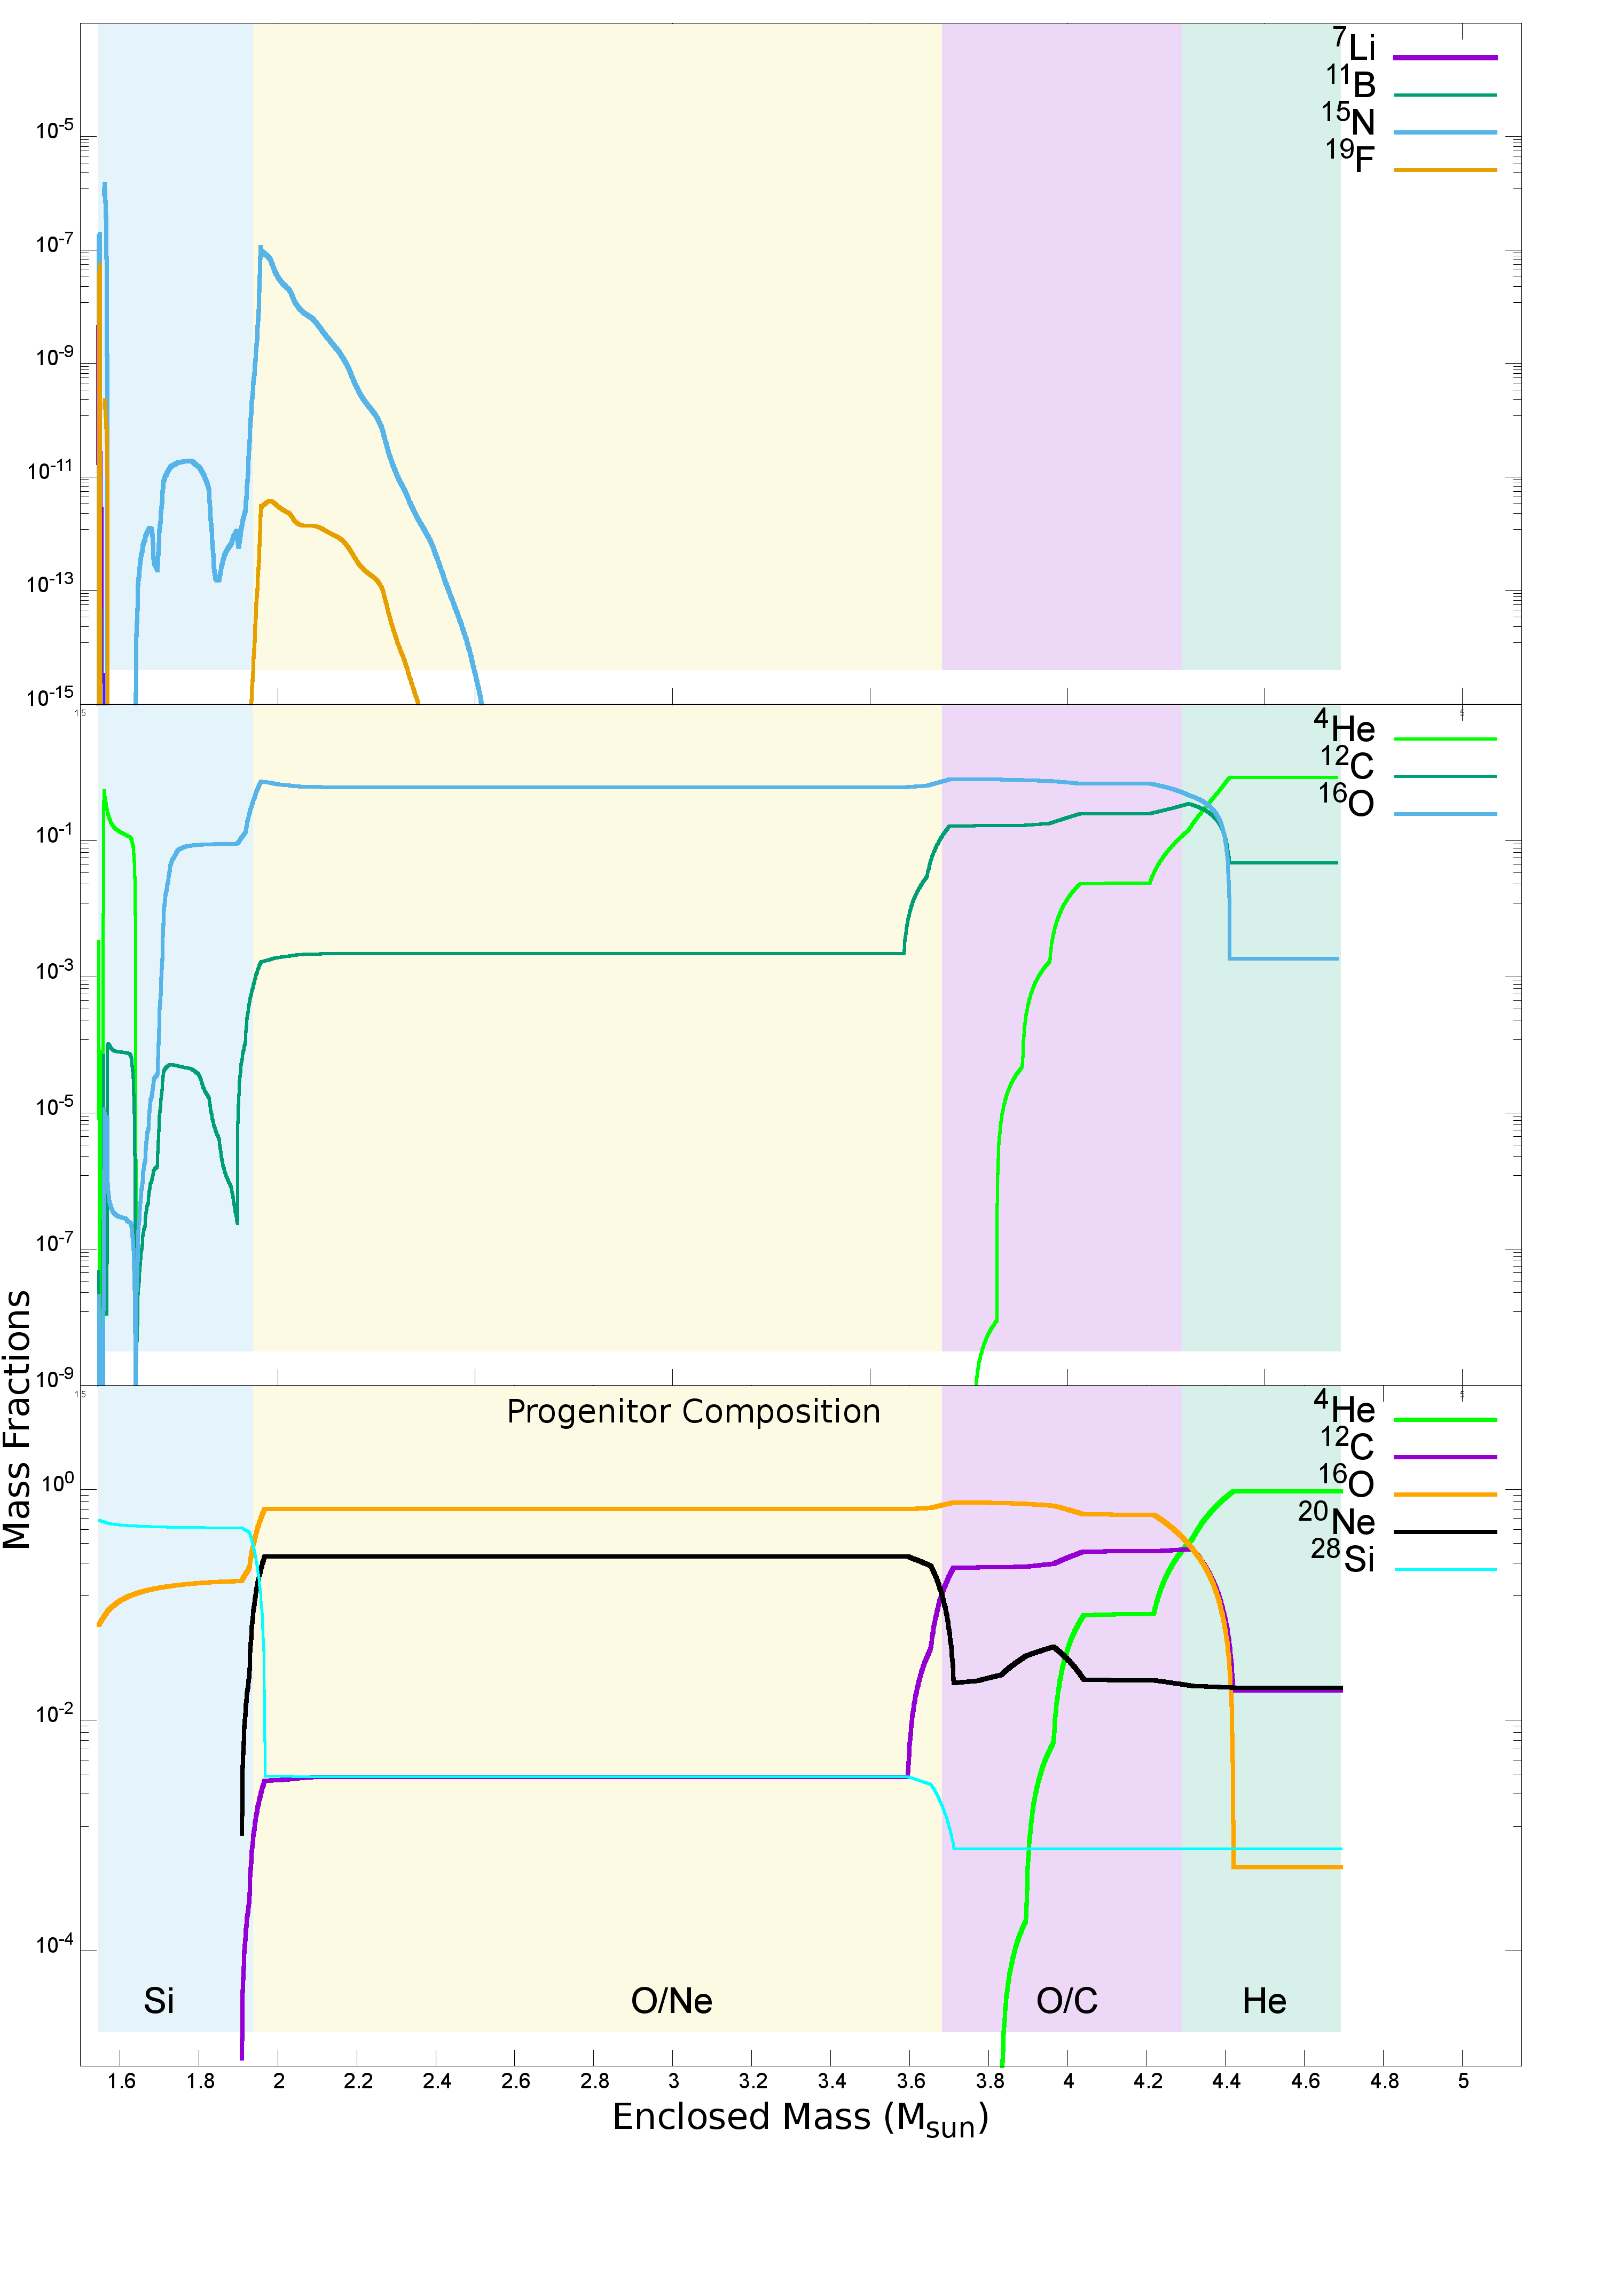
\includegraphics[width=\textwidth]{figures/abundadecay_noNu_he4li7b11c12n15o16f19_hor}
		\caption[Nötrino Sentezlenmesi İhmal Edildiğinde]{Nötrino sentezlenmesi ihmal edildiğinde}
	\end{subfigure}
%%%%%%%%%%%%%%
	\begin{subfigure}{.49\textwidth}
		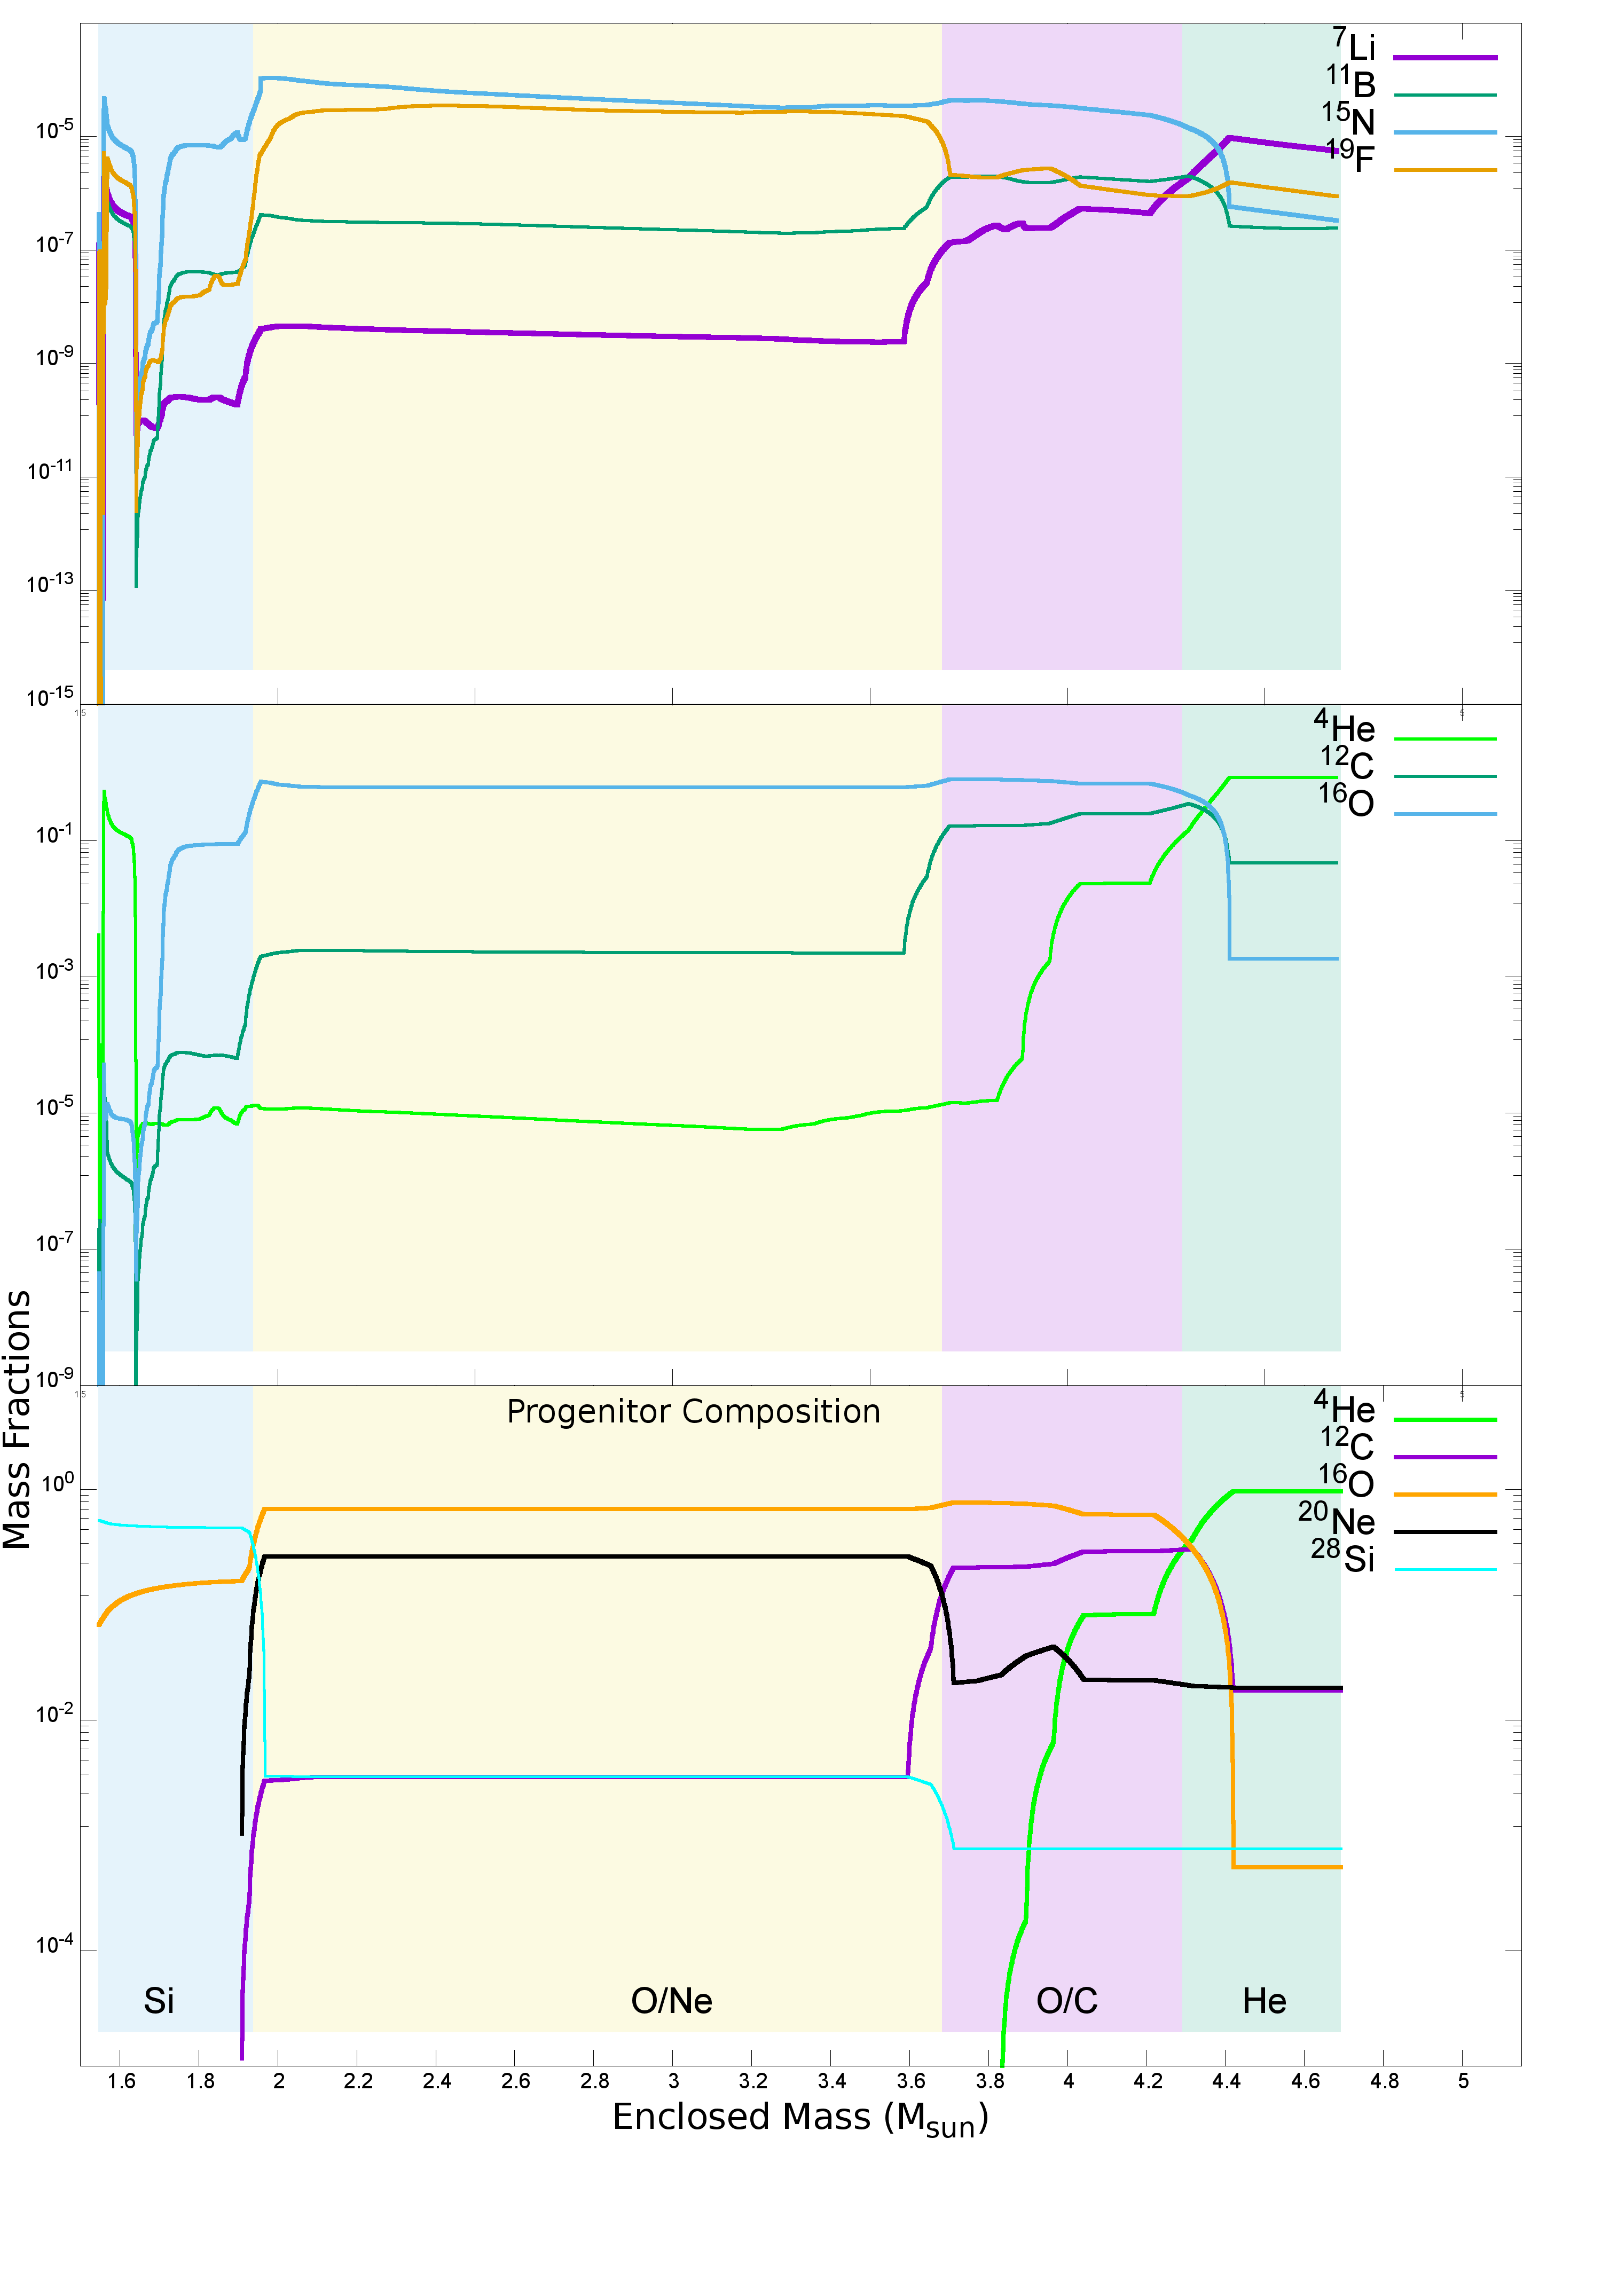
\includegraphics[width=\textwidth]{figures/abundadecay_he4li7b11c12n15o16f19_hor}
		\caption[Nötrino Sentezlenmesi Dahil Edildiğinde]{Nötrino sentezlenmesi dahil edildiğinde.}
	\end{subfigure}
%%%%%%%%%%%%%%
	\caption[Nötrinolu Ve Nötrinosuz Nötrino-işlem Çekirdeklerinin Kütle Kesirleri]{Nötrinolu ve nötrinosuz nötrino-işlem çekirdeklerinin kütle kesirleri.}
    \label{fig:he4li7b11c12n15o16f19_abund_comp}
\end{figure}

$18.8$ M$ _{\odot} $ kütleli PUSHing simülasyonu kullanılarak elde edilen bazı $ \nu $-işlem çekirdeklerinin, $ ^{7} $Li, $ ^{11} $B, $ ^{15} $N ve $ ^{19} $F, kütle kesirleri \ref{fig:he4li7b11c12n15o16f19_abund_comp} numaralı şekillerde verilmiştir. Bu şekillerde, nötrinolu ve nötrinosuz çekirdek sentezi arasındaki fark, O/Ne, O/C ve He kabuklarında açıkça gözükmektedir. Nötrino etkileşimleri dikkate alınmaz ise, yıldız içerisinde $ ^{7} $Li ve $ ^{11} $B izotopu sentezlenemez. Bu çekirdeklere ek olarak $ ^{15} $N ve $ ^{19} $F üretimi de nötrino varlığından etkilenir. Nötrino işlemi, bu çekirdeklerin üretimine $ ^{16} $O($ \nu $,$ \nu $'$ p/n $)$ ^{15} $N ve $ ^{20} $Ne($ \nu $,$ \nu $'$ p/n $)$ ^{19} $F tepkimeleri ile katkıda bulunur.

Şekillerdeki tüm kütle fraksiyonları değerleri, bozunmaların ardından elde edildiğini söylemek önemlidir. Bu, çekirdek sentezleme simülasyonun bitip $200$ saniye sonrasına kadar bozunma hesaplamalarının dahil edildiği anlamına gelir. Son olarak \ref{fig:he4li7b11c12n15o16f19_abund_comp} numaralı şekilde, nötrinoların O/Ne katmanında önemli miktarda $ ^{4} $He yani $ \alpha $ parçacıkları ürettiği görülür. Süpernova evrim simülasyonu $5$ saniye sürdüğü ve o anda şok dalgası O/Ne tabakasının sonuna ulaştığı için bu bölgedeki bolluklar nötrino işlem veya diğer tip işlem (n,p,$\nu$ p gibi) etkileşimlerle kolayca açıklanamaz. Şok dalgasının enerjisi ile bu noktadaki çekirdekler de parçalanır. Yani parçalanma (spallation) reaksiyonları çekirdek bolluğu ve çekirdek sentezleme hesaplarında önemli yer tutar. Bu çalışmada parçalanma etkisi dikkate alınmıştır.

Yük sayıları (charge number) göre tüm çekirdeklerin toplam ürünleri (yield) \ref{fig:abundadecay_Z_TotalYields_nu_nuNo} numaralı şekilde verilmiştir. Nötrino-çekirdek etkileşimleri çoğunlukla Li, Be, B ve F elementlerinin ve bunların izotoplarının üretimini önemli ölçüde etkiler. Tüm ürünler, kararsız $ ^{7} $Be ve $ ^{11} $C çekirdeklerinin bozunumundan önce hesaplanmıştır. \ref{fig:abundadecay_Z_TotalYields_nu_nuNo} numaralı şekilde, $ Z=4 $ ve $ Z=9 $ civarındaki ani artış, nötrino sürecinin kırılgan hafif elementlerin Güneş sistemindeki bolluğunu açıklamada umut vericidir. Ayrıca nötrino etkileşimleri yoluyla Be çekirdeğinin üretilmesi, Li ve B çekirdeklerinin toplam verimini değiştirir. Bunun iki nedeni vardır. Bunlardan en önemlisi, nötrinoların Be çekirdeğindeki proton/nötron sayısını değiştirmesi ve bunun sonucundaki beta bozunumlarıdır. Bir diğeri ise nötrinolar, yüksüz akım etkileşimleri yoluyla enerjilerini yıldız ortamına aktarmalarıdır. Bu aktarım elementlerin reaksiyon hızını da arttırır. Son olarak $ Z=50 $'nin ötesindeki küçük değişiklikler önemli değildir çünkü ata yıldızın bileşeninde ağır elementleri üretebilecek olan ağır izotoplar bulunmamaktadır.

\begin{figure}[hbt!]
    \centering
    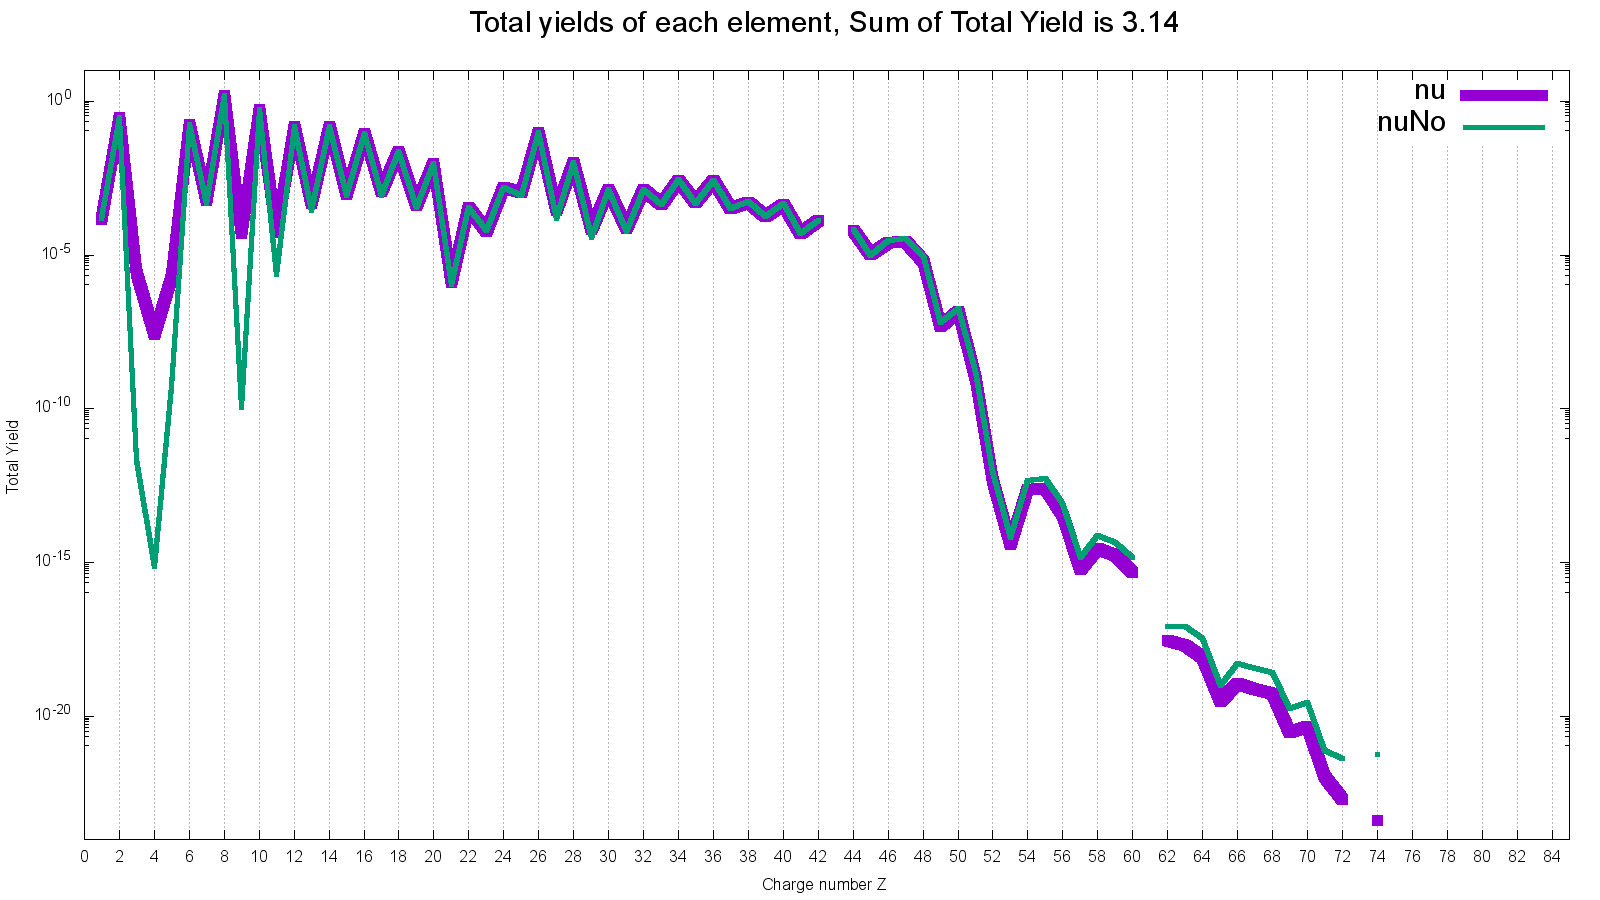
\includegraphics[width=1\textwidth]{figures/abundadecay_Z_TotalYields_nu_nuNo}
    \caption[Toplam Ürünün Yük Sayısı $ Z $'ye Göre Değişimi.]{Toplam ürünün yük sayısı $ Z $'ye göre değişimi. \emph{Nu} ile adlandırılan mor çizgiler nötrino etkileşimleri gözetildiğinde açığa çıkan toplam ürünleri, \emph{nuNo}" ise nötrino etkileşimlerinin ihmal edildiği durumda açığa çıkan toplam ürünleri gösterir.}
    \label{fig:abundadecay_Z_TotalYields_nu_nuNo}
\end{figure}
\newpage
\chapter{SONUÇ}\label{ch:sonuc}
\paragraph{}
Bu çalışmada, nötrinoların kollektif çeşni evriminin, nötrino elektromanyetik alan etkileşimi varlığında nasıl değiştiğini hem analitik olarak hem de sayısal olarak inceledik. Elde ettiğimiz analitik sonuçların ÇÇSN soğuma evresinin erken dönemi için tutarlı ve doğru sonuç verdiğini gördük. ÇÇSN meydana geldikten yaklaşık $ 3-4 $ saniye sonra, MSW ve SFP rezonanslarının gerçekleştiği uzaklıklar yakınlaştığı için iki çeşniye indirgenmiş analitik çözümler ile sayısal çözümler arasında farklılıklar ortaya çıkmaktadır. Faz etkileri ile kendisini gösteren bu farklılık yüksek enerjili nötrinolarda daha belirgin hale gelmektedir.

Yaptığımız çalışmayı özetlersek, öncelikle nötrinoların manyetik alan ve madde etkileşimleri altında çeşni evrimini veren hareket denklemlerini yazdık. Bu denklemleri iki farklı şekilde çözdük. Birincisi, manyetik alanın etkisini tedirgenmiş bir potansiyel olarak alıp evrimin özvektörlerini elde ettik. Bu özvektörlere karşılık gelen özdeğer katkılarını hesapladık. Ardından eksponansiyel olarak değişen baryon yoğunluğu ve sabit manyetik alan altında, iki çeşniye indirgenmiş hareket denklemlerinin çözümünün konfluent hipergeometrik fonksiyonlar olduğunu elde ettik. Ayrıca manyetik alanın baryon yoğunluğu ile aynı eksponansiyel azalmaya sahip olduğunda, çözümlerinin genelleştirilmiş hipergeometrik fonksiyonlar ve birleşmiş Laguerre polinomları cinsinden verildiğini bulduk.

ÇÇSN içerisindeki çeşni evrimini incelemek adına oyuncak modeller kurduk. Bunun için yoğunluk operatörünün özbazdaki analitik ifadesini, LZ geçiş olasılıkları ve fazların katkısını da dahil ederek yazdık. Yoğunluk operatörüne sırayla salınım fazını, SFP rezonansından kaynaklanan LZ geçiş olasılığını ve bunun fazını ve son olarak MSW rezonansından kaynaklanan LZ geçiş olasılığını ve bunun fazını ekledik. Elde ettiğimiz ifadeyi \emph{ortalamadan} sorumlu, \emph{hatadan} sorumlu ve \emph{salınımdan} sorumlu terim  olarak üçe ayırdık. Sonsuz uzaklıkta salınımdan sorumlu terim sıfıra gideceği için bu terimi hesaba katmadık. Tümüyle adyabatik evrim olması durumunda, fazlardan gelen katkıların yani hatadan sorumlu olan terimin sıfır olacağını elde ettik. Hatadan sorumlu kısma gelen tüm katkılar nötrinoların rezonanslara farklı fazlarla girmelerinden kaynaklanır ve bunlar sadece geçişleri adyabatik olmadığında kendini gösterir. Bu etkiyi daha iyi gözlemleyebilmek için adyabatik olmayan ÇÇSN'ya ait başlangıç koşullarında küçük değişiklikler yapıp fazların etkisini ortaya çıkardık. SFP ve MSW rezonansının birbirinden yeteri kadar ayrıldığı çeşni evrimde faz etkileri, analitik öngörülerimzle tam olarak uyumlu çıkmaktadır. Burada bahsettiğimiz "yeteri kadar" kavramını niceliksel olarak tanımladık ve rezonans noktalarındaki $ \sin^{2}(2\theta) $ teriminden yarım uzunluk yarım maksimum değerlerini analitik olarak elde ettik. Yaptığımız analizler sonucunda ÇÇSN meydana geldikten yaklaşık $ 3-4 $ saniye sonra MSW ve SFP rezonansının birbirine yaklaştığını ve üç çeşni etkilerin ortaya çıktığını bulduk. Yoğunluk operatörünün hatadan sorumlu kısmı, başlangıçta Hamiltonyen'in enerji özdurumlarının çeşni özdurumları olmaktan ne kadar uzak olduğuna da bağlıdır. Bu da doğrudan $ \mu B $ teriminin madde potansiyeline göre ne kadar güçlü olduğuna bağlıdır. Buna göre $ \mu $ ya da $ B $ artacak olursa gözlemsel belirsizlik de artacaktır.

Analitik çözümler ile sayısal çözümleri karşılaştırmamızın ardından gerçekçi ÇÇSN modeli için simülasyon yaptık. Elektromanyetik etkileşimlerin ve nötrino öz-kırılımının çeşni evrimine olan etkilerine bakmak için dört ayrı model ile çalıştık. Elektromanyetik etkileşimlerin $ x $ antinötrino yoğunluğunu arttırdığını bulduk. Ayrıca, bu etkileşimin kollektif nötrino salınımlarından kaynaklanan spektral ayrışmayı belirsizleştirdiğini, hatta antinötrino enerji spektrumunda bulunan spektral ayrışmayı yok ettiğini gözlemledik.

Bu tezin son bölümünde ise nötrino işlemi çekirdek sentezlenme sonucunda $ ^{7} $Li ve $ ^{11} $B gibi nötrino-işlem elementlerinin kütle kesirleri elde edilmiştir. Nötrino etkileşimlerinin toplam ürün üzerindeki etkisine bakılmıştır. Çekirdek sentezleme hesapları yapılırken nötrino işlemi dikkate alınırsa Lityum elementi $ 10^{10} $ kat, Bor elementi ise $ 10^{5} $ kat daha bol bulunacaktır.

Tüm nötrino-işlem hesapları, başka ata yıldız modelleri ve onlara uygun süpernova simülasyonları kullanılarak yapılabilir. İstatistik arttırılarak, Güneş sistemindeki element bollukları bu yolla açıklanabilir. Ayrıca iki major nötrino-işlem element üretim mekanizması anlaşılmasının ardından Güneş sistemi ile daha sağlıklı karşılaştırma olanağı bulabiliriz. 

Bu çalışmanın bir sonraki adımı SFP ile MSW rezonansı arasında kalan donmuş fazların çeşni evrimine olan katkısını incelemektir. Elektron kesrinin aniden değiştiği Yıldız'ın iç bölgelerinde nötrino enerji spektrumu, donmuş fazlardan dolayı spektral ayrışmaya benzer bir davranışta bulunacaktır. Ayrıca bu bölge, nötrino öz-kırılım etkilerinin de meydana geldiği bölge olduğu için birden fazla spektral ayrışmanın meydana gelmesi muhtemeldir.

%\addcontentsline{toc}{chapter}{KAYNAKLAR}
\bibliographystyle{ieeetr}
\bibliography{taygunTezKaynaklar}	

\begin{appendices}
\chapter{Bloch Vektörü}
\paragraph{}
Bu bölümde, Hamiltonyen matrisinden Bloch vektörü ve ilgili büyüklükler elde edilecektir. Bloch vektörü, iki seviyeli saf (pure) kuantum mekaniksel bir sistemin geometrik temsilini anlamamıza yardımcı olur. \emph{Bloch} ismi, Nobel ödüllü Felix Bloch'dan gelmektedir \cite{Bloch:1946zza}. Spin ve izospin gibi ikili kuantum mekaniksel sistemlerin analizi ve yoğunluk matrisinin davranışını anlamak için ortaya konan Bloch küresi ve Bloch vektörü, matematiksel özellikleri nedeniyle başka alanlarda da kullanılır. Biz, Hamiltonyen'in özdeğerlerini, özvektörlerini, ölçülebilirlerini ve özbaza döndüren açıyı bulmak için Bloch vektöründen yararlanacağız. Bloch vektör tanımı Hamiltonyen'den bağımsız herhangi bir $ 2 \times 2 $ sanal matris için de yazılabilir.
\begin{align}
\nonumber H_{\alpha\beta} &= \mqty(H_{ee} & H_{ex} \\ H_{xe} & H_{xx}) \text{ ,}\\
\nonumber				   &= \frac{H_{ee} + H_{xx}}{2} I + \frac{1}{2} \mqty(H_{ee} - H_{xx} & 2 H_{ex}\\ 2 H_{xe} & H_{xx}-H_{ee})  \text{ ,}\\
						   &= k I + \frac{1}{2} \vec{\sigma} \cdot \vec{B} \text{.}
\end{align}

Evrime katkı sağlamayan ve birim matrisle orantılı olan $ kI $ terimini ayrı yazdık. $ k $ katsayısı, Hamiltonyen matrisinin köşegen elemanlarının toplamının yarısıdır ve $ I $ matrisi ise $2$ boyutlu birim matristir. Denklemde $ \vec{\sigma} $ Pauli-spin matris vektörüdür. $ \vec{B} $ ise \emph{Bloch vektörüdür} ve aşağıdaki gibi tanımlanır.
\begin{equation}\label{eqn:appBloch_B_Hmat}
    \vec{B} = \mqty(H_{ex} & 0 & [H_{ee}-H_{xx}]/2 ) \text{ .}
\end{equation}

Bloch vektörü kullanılarak özdeğerler ve özvektörler kolayca yazılabilir. Özdeğerler aşağıdaki gibidir.
\begin{align} \label{eqn:appBloch_B_Ozdeg}
    \lambda_{1} = k + \abs{\vec{B}} \text{ ,}\\
    \lambda_{2} = k - \abs{\vec{B}} \text{ .}
\end{align}
Bu özdeğerlere karşılık gelen özvektörler de Bloch vektörünün elemanları cinsinden yazılabilir.
\begin{align}
    \vec{v}_{1} =& \mqty(B_{x} - iB_{y} \\ \abs{\vec{B}} - B_{z}) \text{ ,}\\
    \vec{v}_{2} =& \mqty(B_{x} - iB_{y} \\ -\abs{\vec{B}} - B_{z}) \text{ .}
\end{align}

Bloch vektörleri yardımıyla sistemin geometrik gösterimi yapılabilir. İlgilendiğimiz sistemlerde Hamiltonyen gerçel (reel) olduğundan dolayı Bloch vektörünün $ y $ bileşeni sıfırdır. Bu da $ \vec{B} $ vektörünü $ x-z $ düzlemine iz düşürür. 
\begin{figure}[!hbt]
	\centering
    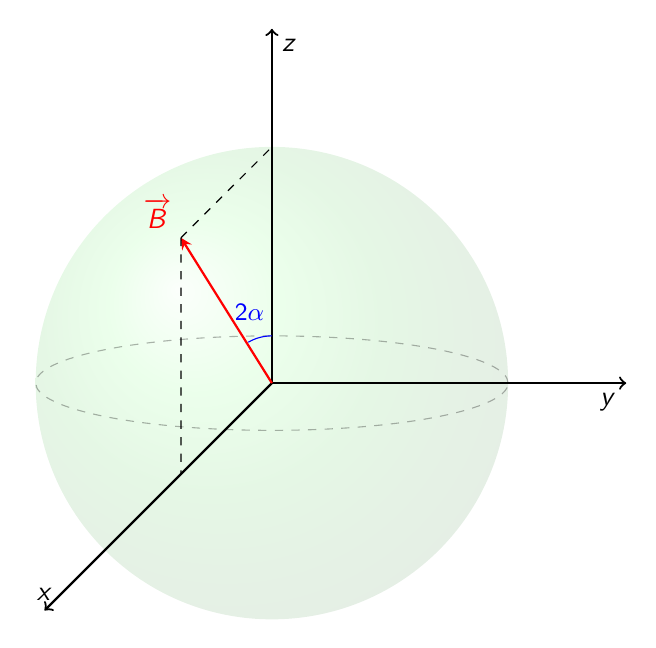
\begin{tikzpicture}[font = \sansmath, scale=1.5]
\coordinate (O) at (0,0,0);
\coordinate (B) at (0,2,2);

% ball background color
\shade[ball color = green, opacity = 0.1] (0,0) circle [radius = 2cm];

% Coordinate System
\draw[thick,->] (0,0,0) -- (3,0,0) node[anchor=north east]{$y$};
\draw[thick,->] (0,0,0) -- (0,3,0) node[anchor=north west]{$z$};
\draw[thick,->] (0,0,0) -- (0,0,5) node[anchor=south]{$x$};

% ellipse at center
\draw[dashed, color=black, opacity = 0.3] (0,0) ellipse ({2} and {0.4});

%draw a vector from origin to point (P) 
\draw[thick,-stealth,color=red] (O) -- (B);

%draw projection on xy plane, and a connecting line
\draw[dashed, color=black] (B) -- (0,0,2);
\draw[dashed, color=black] (B) -- (0,2,0);

% Text
\node[anchor=south east, color=red] at (0,2,2) {$\overrightarrow{B} $};

%draw theta arc and label, using rotated coordinate system
\draw[color = blue] (0cm,0.4cm) arc (90:120:0.4cm);
% Text
\node[anchor=south, color=blue] at (0,0.6,0.4) {$$\small $2\alpha$ $$};
  
\end{tikzpicture}
    \caption[Bloch Küresi ve Bloch Vektörü]{Bloch Küresi ve Bloch Vektörü}
    \label{fig:blochVec}%
\end{figure}

Nötrino salınımlarında, bir bazdan diğer baza geçerken dönme matrisleri $ \mathcal{R}_{\theta} $ kullanılır. Bloch vektörü $ \vec{B} $ ile $ z $-ekseni arasında açı karışım açısının iki katı olarak tanımlanır. Bu tanım altında Bloch vektörünün bileşenleri $ B_{x} = \abs{\vec{B}}\sin 2\alpha $, $ B_{y}=0 $ ve $ B_{z} = \abs{\vec{B}} \cos 2\alpha $ şeklinde yazılır. Özvektörler de karışım açısı $ \alpha $ cinsinden yazılabilir. Boşluk salınımları ile karşılaştırdığımızda $ \alpha $ açısı ile $ \theta $ açısı eş değerdir.
\begin{align} \label{eqn:appBloch_B_Ozvec}
    \vec{v}_{1} =& 2 \abs{\vec{B}} \sin \alpha \mqty(\cos \alpha \\ \sin \alpha) \text{ ,}\\
    \vec{v}_{2} =& 2 \abs{\vec{B}} \cos \alpha -\mqty(\sin \alpha \\-\cos \alpha) \text{ .}
\end{align}
Özvektörlerin başındaki katsayı, normalizasyon katsayısıdır.

\eqref{eqn:appBloch_B_Hmat} numaralı denklem, matris notasyonu kullanılarak elde edilmiştir. Benzer işlemleri ve denklemleri Hamiltonyen operatörünün bileşenleri için de yazabiliriz.
\begin{equation} \label{eqn:appBloch_B}
    \vec{B} = \mqty(\mel{\nu_{e}}{\hat{H}}{\nu_{x}} & 0 & (\mel{\nu_{e}}{\hat{H}}{\nu_{e}} - \mel{\nu_{x}}{\hat{H}}{\nu_{x}})/2  ) \text{ .}
\end{equation}

Bloch vektörü, Hamiltonyen'in hangi bazda yazıldığına göre değişir \cite{Pehlivan:2011hp}. \eqref{eqn:appBloch_B} numaralı denklemde çeşni bazı kullanılarak yazılmıştır. Bloch vektörünün $ z $-ekseni ile arasındaki açı $ 2\alpha $ ise aşağıdaki gibi belirlenir.
\begin{equation} \label{eqn:appBloch_mixAng}
\cos 2\alpha = \frac{B_{z}}{\abs{\vec{B}}} \text{ ,} \qquad \sin 2\alpha = \frac{B_{x}}{\abs{\vec{B}}} \text{ .}
\end{equation}

Elde edilen açıların işareti, analitik düzlemde hangi kuadrantta olduğunu belirler. Uygun trigonometrik özdeşlikler ile istenilen kuadranta geçiş yapılır. 

\end{appendices}

\newpage
%\chapter{SONUÇ}
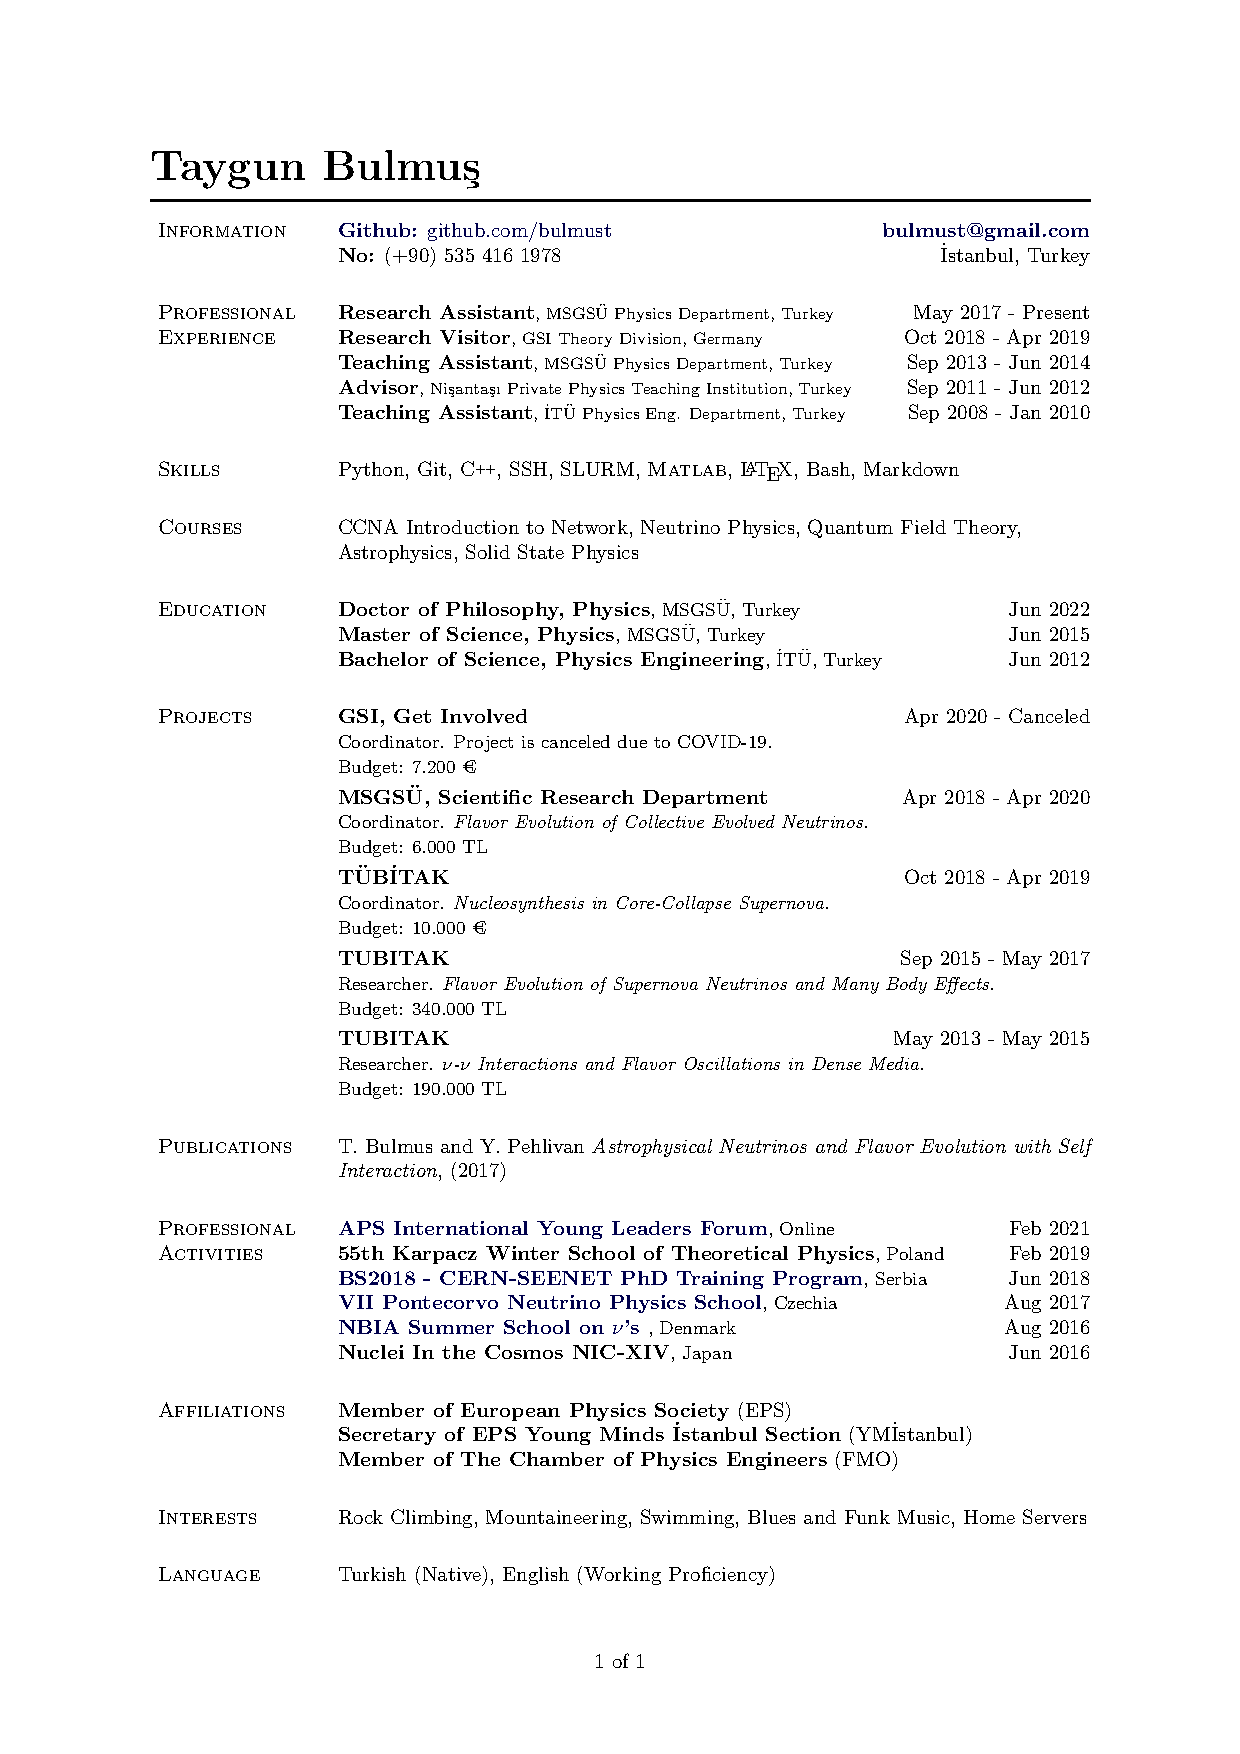
\includepdf[pages=-]{islakImzaliKagitlar/IsmailTaygunBulmus_CV_EN.pdf} 

%%%%%%%%%%%%%%%%%%%%%%%%%%%%%%%%%%%%%%%%%%%%%%%%%%%%%%%%%%%%%%%%%%%%
% Boş Sayfa
%%%%%%%%%%%%%%%%%%%%%%%%%%%%%%%%%%%%%%%%%%%%%%%%%%%%%%%%%%%%%%%%%%%%
\thispagestyle{empty}
\mbox{}
\newpage

\end{document}